\documentclass[11pt, oneside]{article}   	% use "amsart" instead of "article" for AMSLaTeX format
\usepackage{geometry}                		% See geometry.pdf to learn the layout options. There are lots.
\geometry{letterpaper}                   		% ... or a4paper or a5paper or ... 
%\geometry{landscape}                		% Activate for for rotated page geometry
%\usepackage[parfill]{parskip}    		% Activate to begin paragraphs with an empty line rather than an indent
\usepackage{graphicx}				% Use pdf, png, jpg, or eps§ with pdflatex; use eps in DVI mode
% TeX will automatically convert eps --> pdf in pdflatex	
\usepackage{amssymb}
\usepackage{float}
\usepackage[cmex10]{amsmath}
\usepackage{mathrsfs,amsthm}
\usepackage{color}
\def\MFIE{{\mathfrak M}}%
\def\EFIE{{\mathfrak E}}%

%\usepackage[sort&compress]{natbib}

\DeclareMathOperator\erf{erf}
\DeclareMathOperator\Ei{Ei}
\newcommand\bbR{\mathbb R}
\newcommand\bphi{\boldsymbol \phi}
\newcommand\brho{\boldsymbol \rho}
\newcommand\rect{\rm rect}
\newcommand\bs{\boldsymbol s}
\newcommand\bx{\boldsymbol x}
\newcommand\by{\boldsymbol y}
\newcommand\bE{\boldsymbol E}
\newcommand\ds{\boldsymbol ds}
\newcommand\bH{\boldsymbol H}
\newcommand\bF{\boldsymbol F}
\newcommand\bA{\boldsymbol A}
\newcommand\bJ{\boldsymbol J}
\newcommand\bj{\boldsymbol j}
\newcommand\bb{\boldsymbol b}
\newcommand\ba{\boldsymbol a}
\newcommand\bM{\boldsymbol M}
\newcommand\In{\operatorname{inc}}
\newcommand\Sc{\operatorname{scat}}
\newcommand\bn{\boldsymbol n}
\newcommand\br{\boldsymbol r}

\newcommand\bP{\boldsymbol P}
\newcommand\bN{\boldsymbol N}
\newcommand\bQ{\boldsymbol Q}
\newcommand\bX{\boldsymbol X}
\newcommand\bY{\boldsymbol Y}
\newcommand\bV{\boldsymbol V}
\newcommand\bu{\boldsymbol u}
\newcommand\bv{\boldsymbol v}


%%\newcommand\tot{\operatorname{tot}}
\newcommand\tot{\operatorname{}}
%\newtheorem{theorem}{Theorem}
\newtheorem{remark}{Remark}
\newtheorem{definition}{Definition}
\newtheorem{thm}{Theorem}
\newtheorem{lemma}{Lemma}

\newcommand{\Vo}{\mathcal V_0}
\newcommand{\To}{\mathcal T_0}
\newcommand{\Vw}{\mathcal V_\omega}
\newcommand{\Tw}{\mathcal T_\omega}


\title{Notes on Smooth Surfaces}
%\author{Felipe Vico\thanks{Instituto de Telecomunicaciones y Aplicaciones Multimedia (ITEAM), 
%Universidad Polit\` ecnica
%de Val\` encia, 46022 Val\` encia, Spain. {{\em email}: {\sf {felipe.vico@gmail.com,
%}}} } \and
%Leslie Greengard, Michael O'Neil \thanks{Courant Institute of Mathematical Sciences,
%         New York University, 
%         251 Mercer Street,
%         New York, NY 10012-1110.
%{{\em email}: {\sf {greengard@cims.nyu.edu.}}}}
%}

%\date{}							% Activate to display a given date or no date


\begin{document}
\maketitle
%\tableofcontents
%\section{}
%\subsection{}

\section{Comments on the code and calling sequences}

The current version of the code includes:
\begin{itemize}
\item Refinement Algorithm
\item Adaptive Sigma
\item Manas' FMM call for each Newton call
\item Fast tree code for smooth sigma evaluation (nadadena.f90).
\item Quadratic triangulated skeletons
\end{itemize}

The calling sequence is:

\begin{verbatim}>> gfortran -o Smooth_Surface_Quadratic_swap_FMM_v4 -O3 nadadena.f90 ..\end{verbatim}
\begin{verbatim}.. Smooth_Surface_Quadratic_swap_FMM_v4.f90 tfmm3dlib.a\end{verbatim}
\begin{verbatim}>>./Smooth_Surface_Quadratic_swap_FMM_v4 \end{verbatim}

The refinement algorithm is activated using the variable $n_{refinement}$ inside the file Smooth\_Surface\_Quadratic\_swap\_FMM\_v4.f90. If $n_{refinement}=0$ then there is no refinement, the number of triangles of the resulting smooth surface equals the number of triangles of the skeleton. If $n_{refinement}=1$ then each smooth triangle is divided by $4$. if $n_{refinement}=2$ then each smooth triangle is divided by $4^2$, and so on..

The adaptive sigma for small details is activated using the variable adaptive\_flag. If adaptive\_flag=0 then there is no adaptivity, if adaptive\_flag=1 then there is adaptivity. In general it could be interesting to disable the adaptivity only if the geometry is given by a very small number of triangles, to avoid some distortions

The FMM call is used on each Newton iteration using $iprec=3$.

The fast tree call to evaluate the variable sigma and gradient of sigma is used on each Newton iteration before each FMM call.

There are several variables at the beginning of the program to establish several options:
\newline
\newline

n\_order\_sk:
\newline
\newline

Number of nodes per skeleton. Used as sources in the FMM code, usually $78$ and not changed.
\newline
\newline

n\_order\_sf:
\newline
\newline

Number of nodes on each smooth triangle. You can use $45$ or $78$
\newline
\newline

n\_refinement
\newline
\newline

n\_refinement=$0$ if no refinement, n\_refinement=$1$ to split each smooth triangle into $4$, n\_refinement=$2$ to split each smooth triangle into $4^2$, and so on.. the skeleton (the number of sources in the fmm call is not modified in any case)
\newline
\newline

adaptive\_flag
\newline
\newline

This is to enable adaptivity, if adaptive\_flag=0 then sigma is constant and has an appropriate value commensured with the size of the triangle. If adaptive\_flag=0 then sigma is a smooth function proportional to the size of each triangle of the skeleton 
\newline
\newline

nombre:
\newline
\newline

variable containing the name of the .msh file from GID as input
\newline
\newline

filename:
\newline
\newline

variable containing the name of the .gov file of the output file that will contain the smooth surface.

\begin{verbatim}x0,y0,z0\end{verbatim}

coordinates of a point that should be inside the resulting smooth surface to test the Gauss integral at the end of the process and estimate the accuracy of the smooth surface.


\section{How to generate a valid .msh file with GID}

Next I describe the procedure to make a .msh file with GID compatible with this code:

First create your model (with consistent normals pointing towards the exterior region), then defile the elements of the mesh as Quadratic (see \ref{GID_figure_1}).

\begin{figure}[H]
\begin{center}
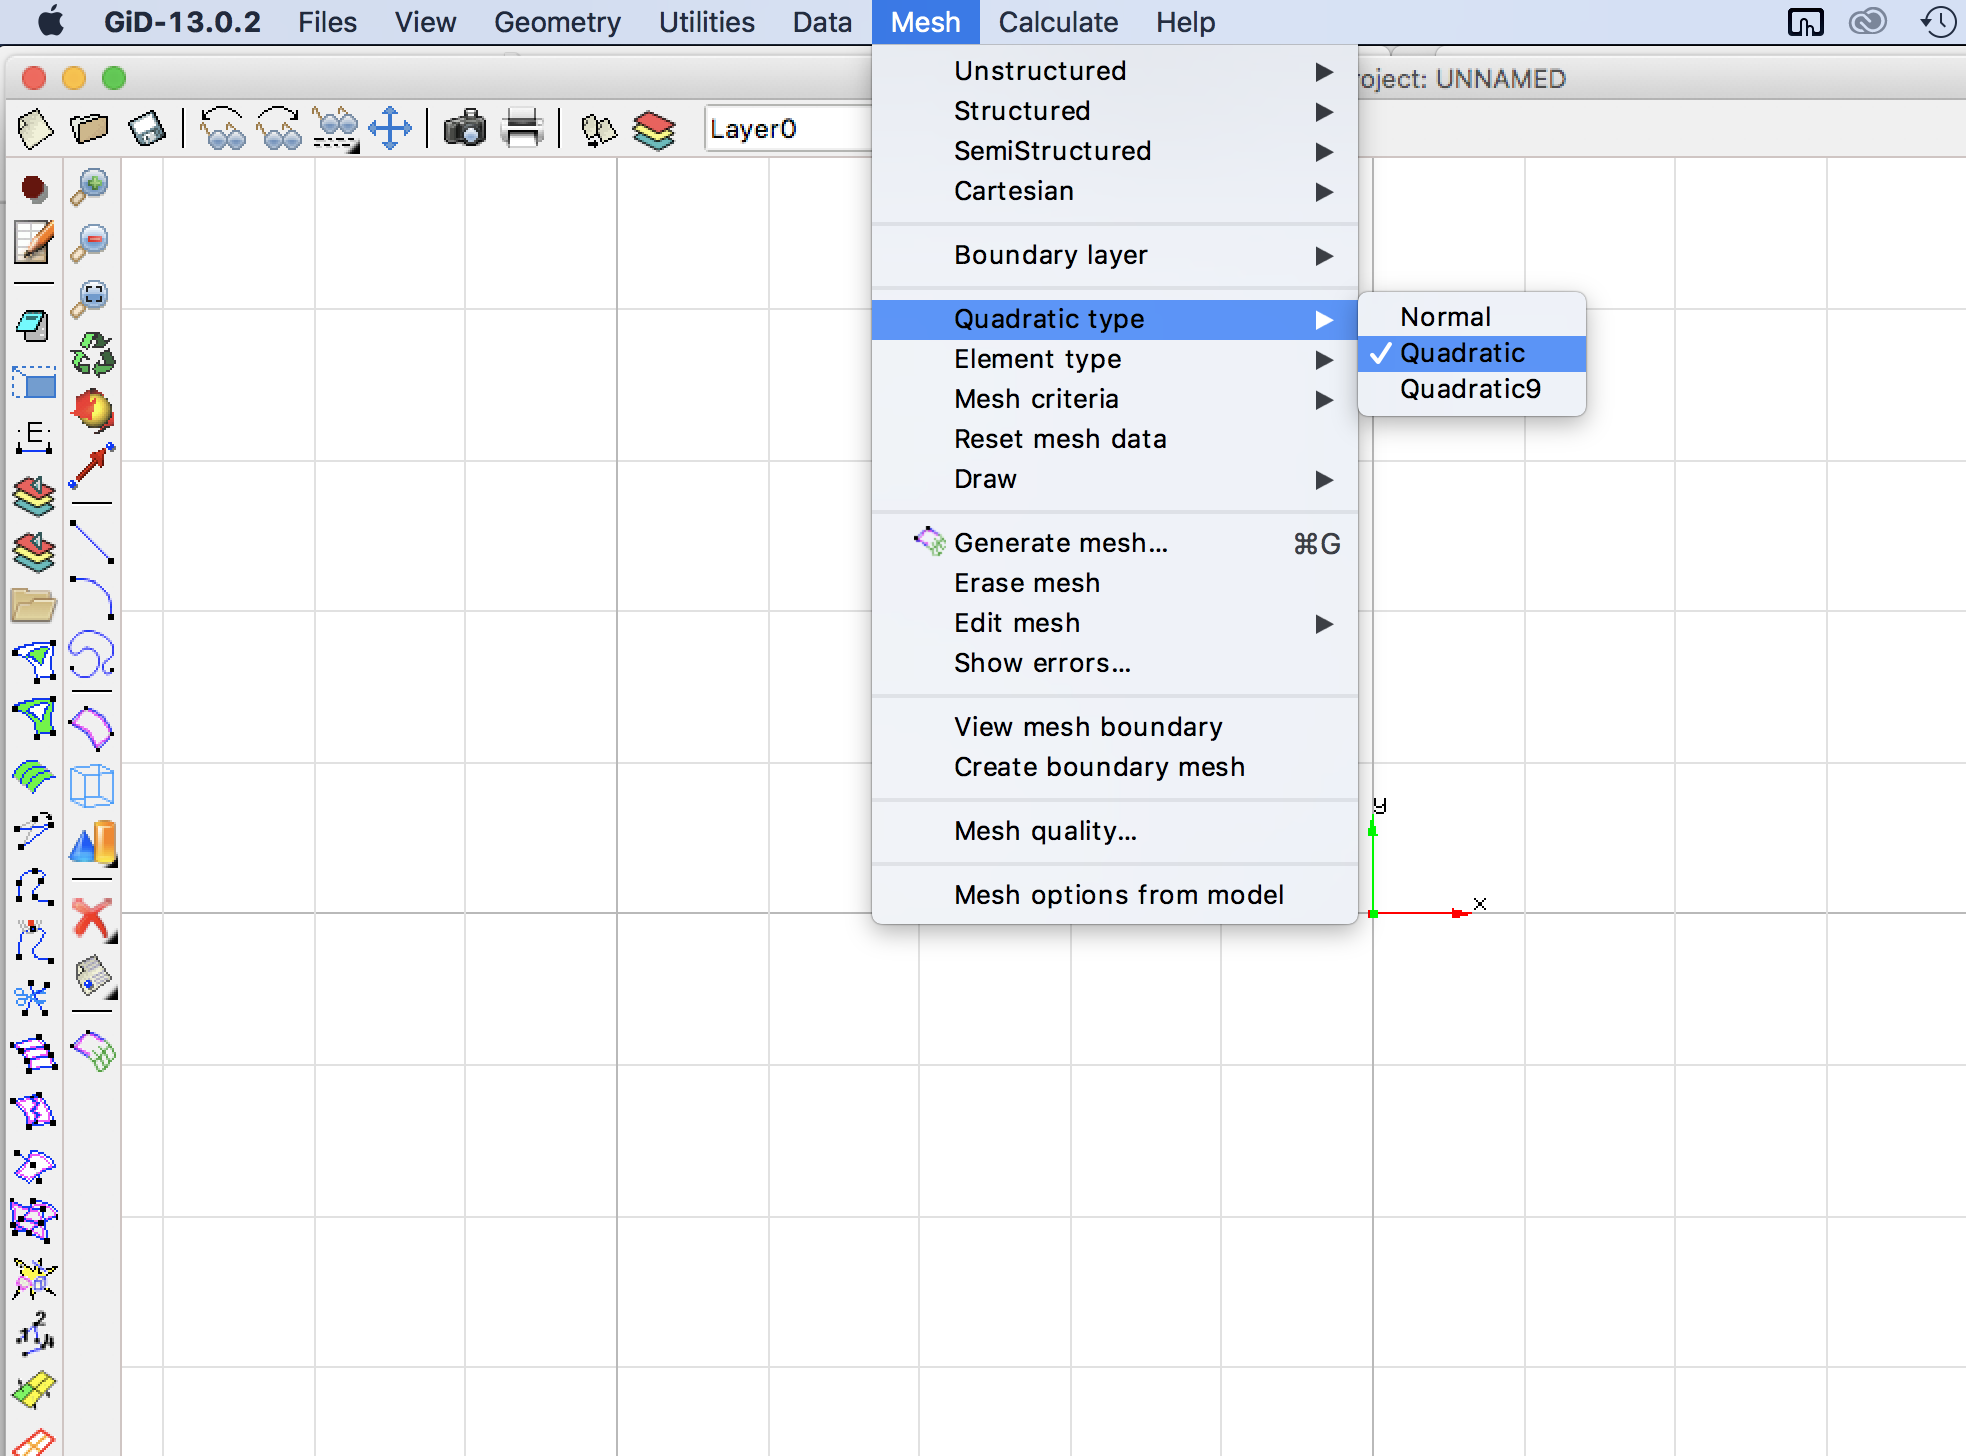
\includegraphics[width=3in]{GID_figure_1.png}%
\end{center}
\caption{}
\label{GID_figure_1}
\end{figure}

Next define the element type as triangles (see \ref{GID_figure_2})

\begin{figure}[H]
\begin{center}
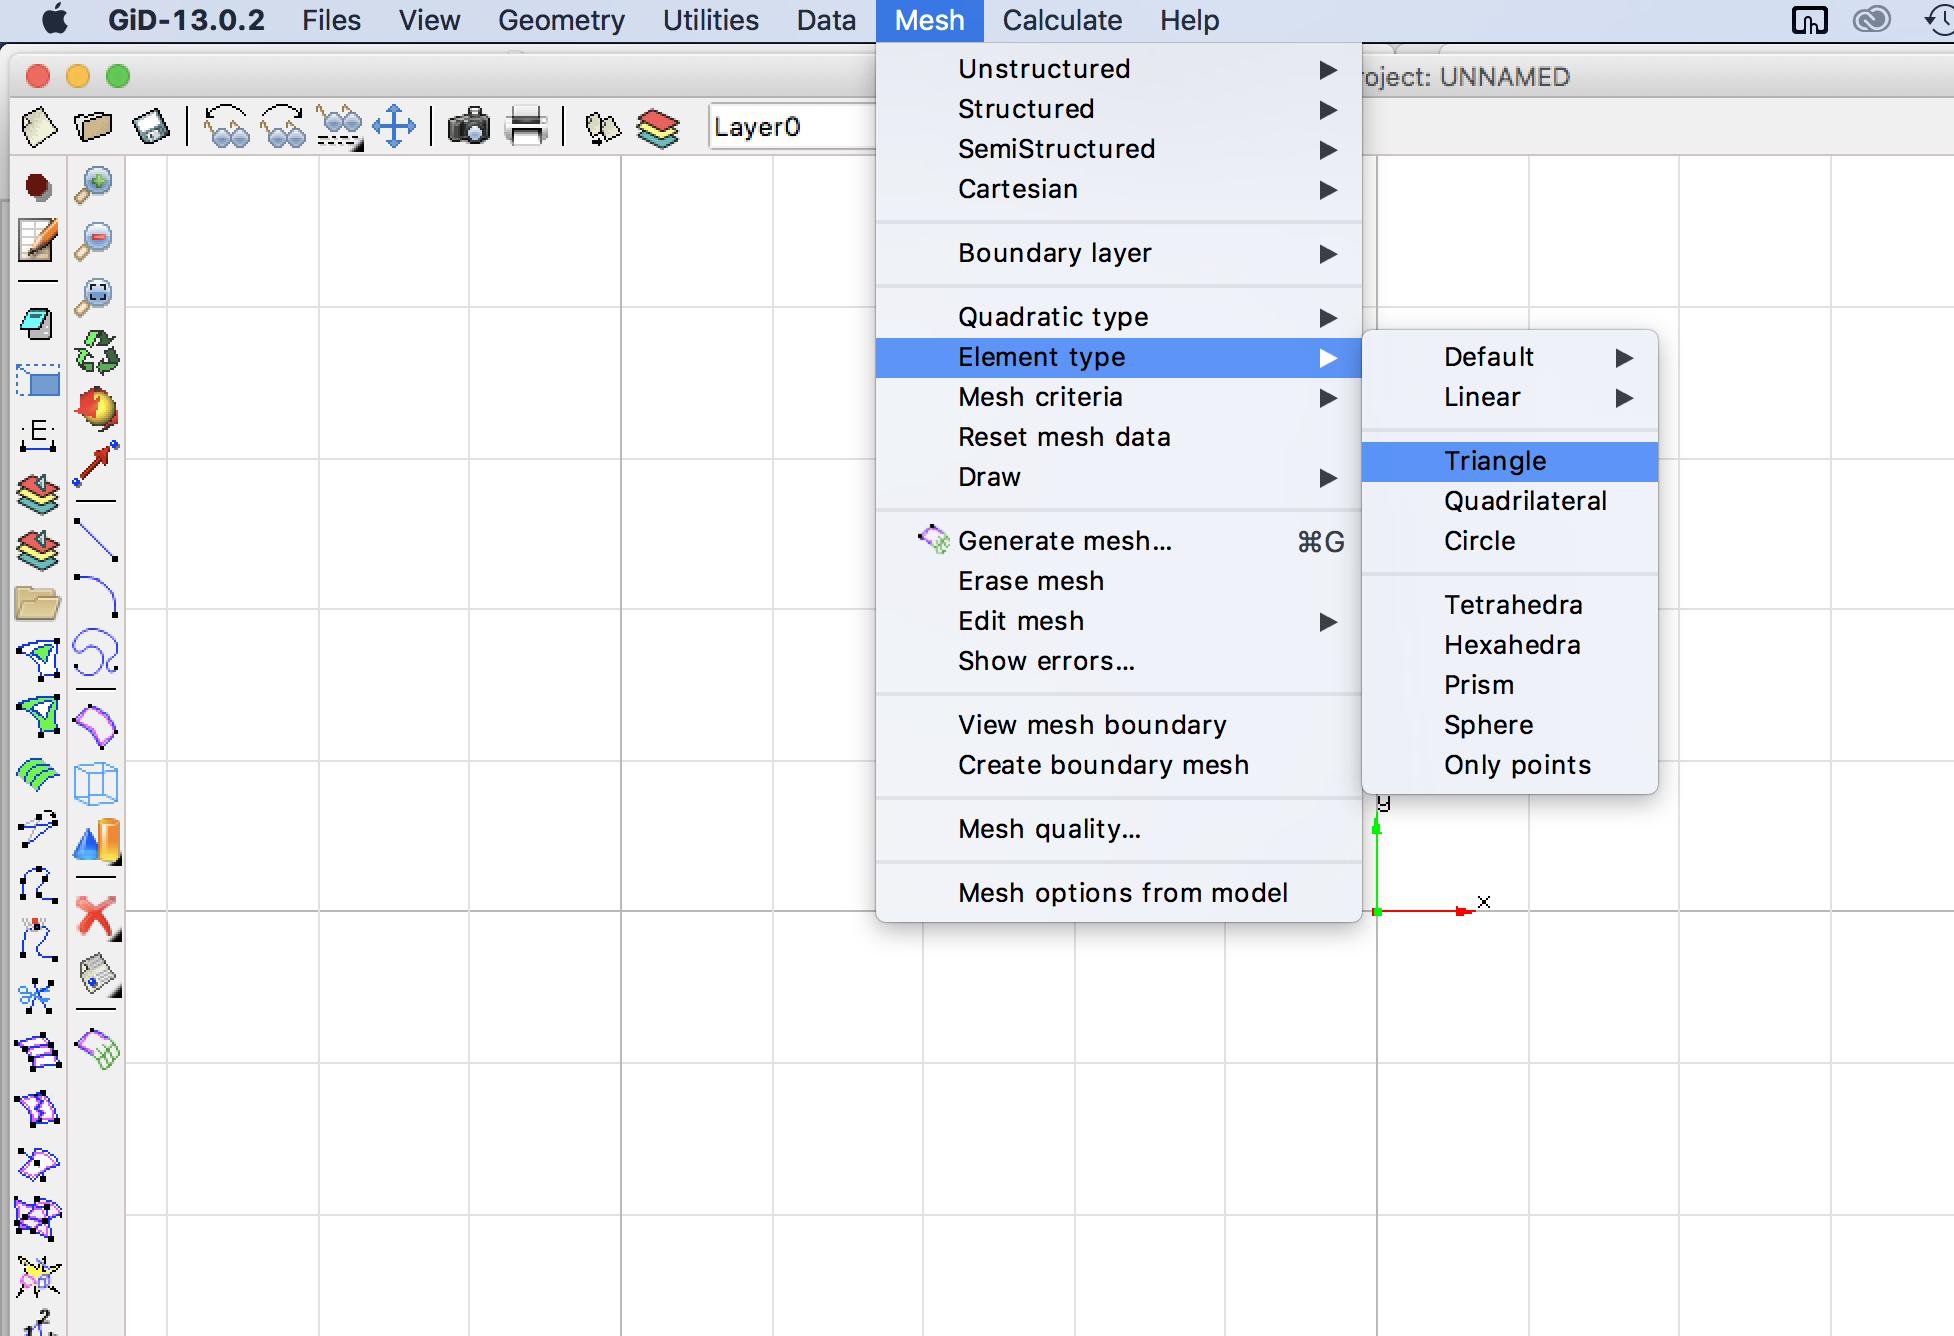
\includegraphics[width=3in]{GID_figure_2.png}%
\end{center}
\caption{}
\label{GID_figure_2}
\end{figure}

and select all the surfaces on the geometry.

Next generate the mesh (see figure \ref{GID_figure_3}) deciding the maximum size of the triangular elements (if there are small details in the geometry, it will create smaller triangles in that region avoiding high differences in size of adjacent triangles) 

\begin{figure}[H]
\begin{center}
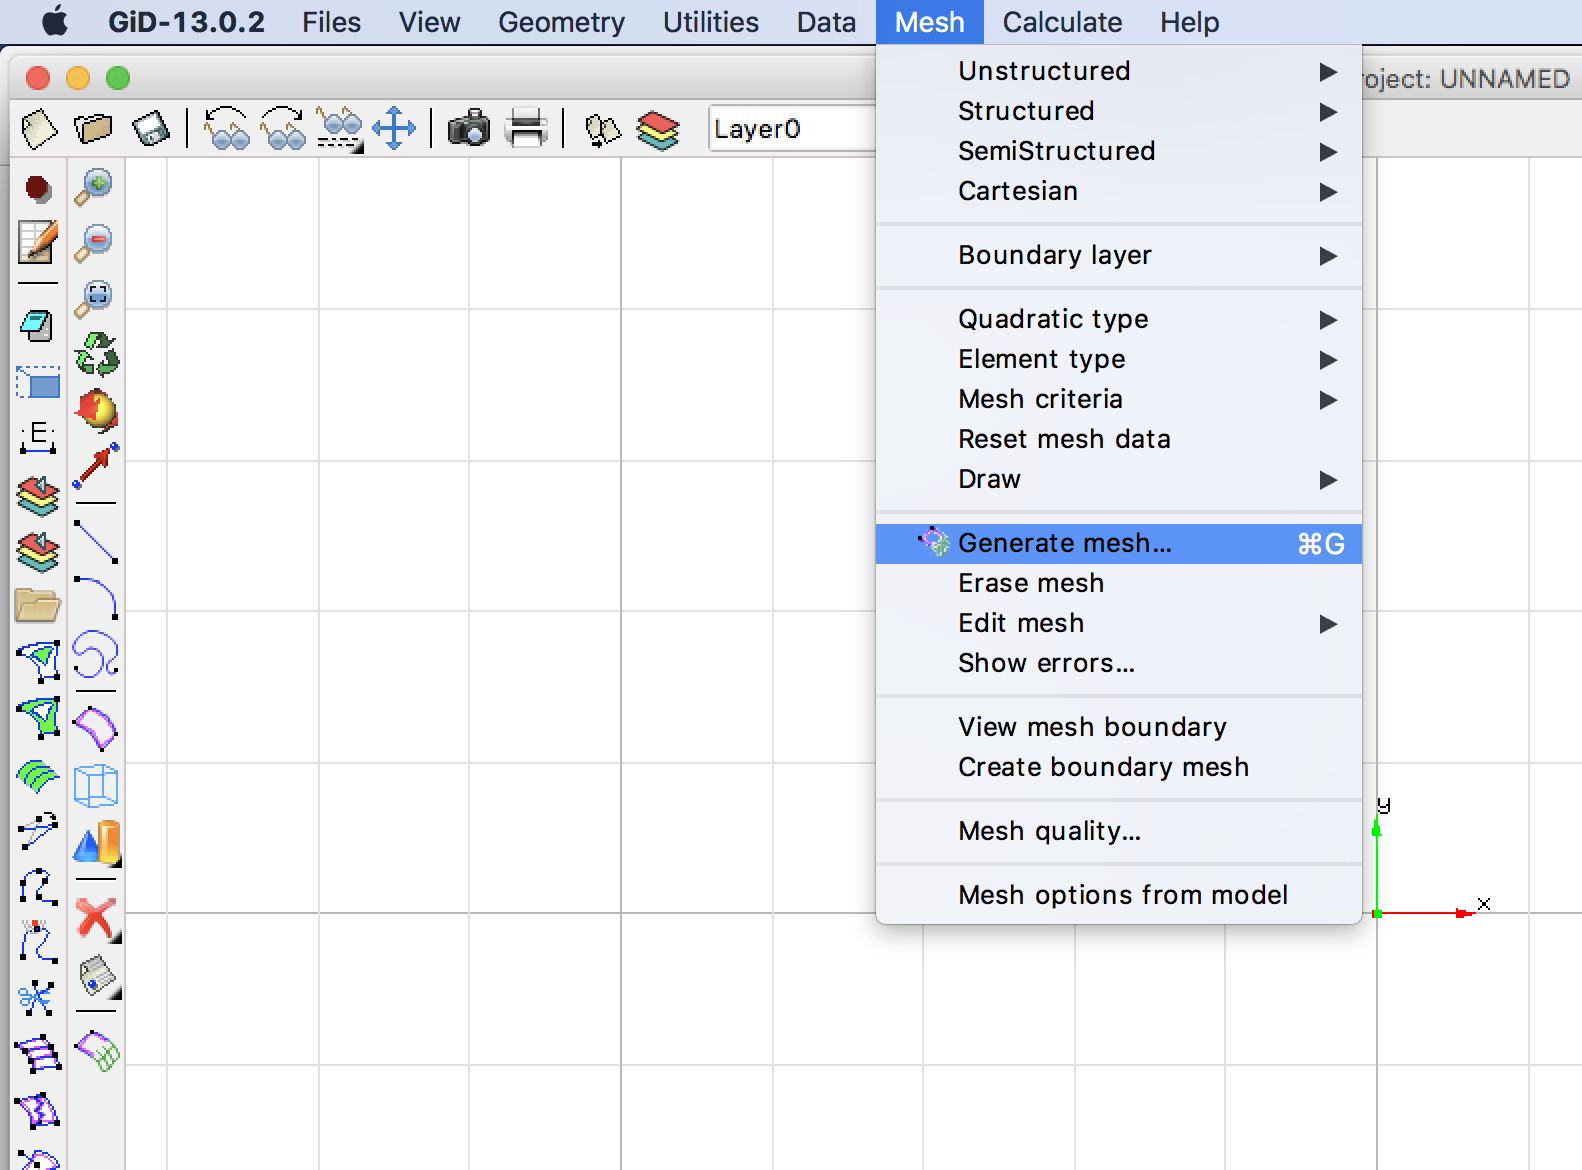
\includegraphics[width=3in]{GID_figure_3.png}%
\end{center}
\caption{}
\label{GID_figure_3}
\end{figure}

Finally save the model using export$>$ASCII project.. (see \ref{GID_figure_4}). 

\begin{figure}[H]
\begin{center}
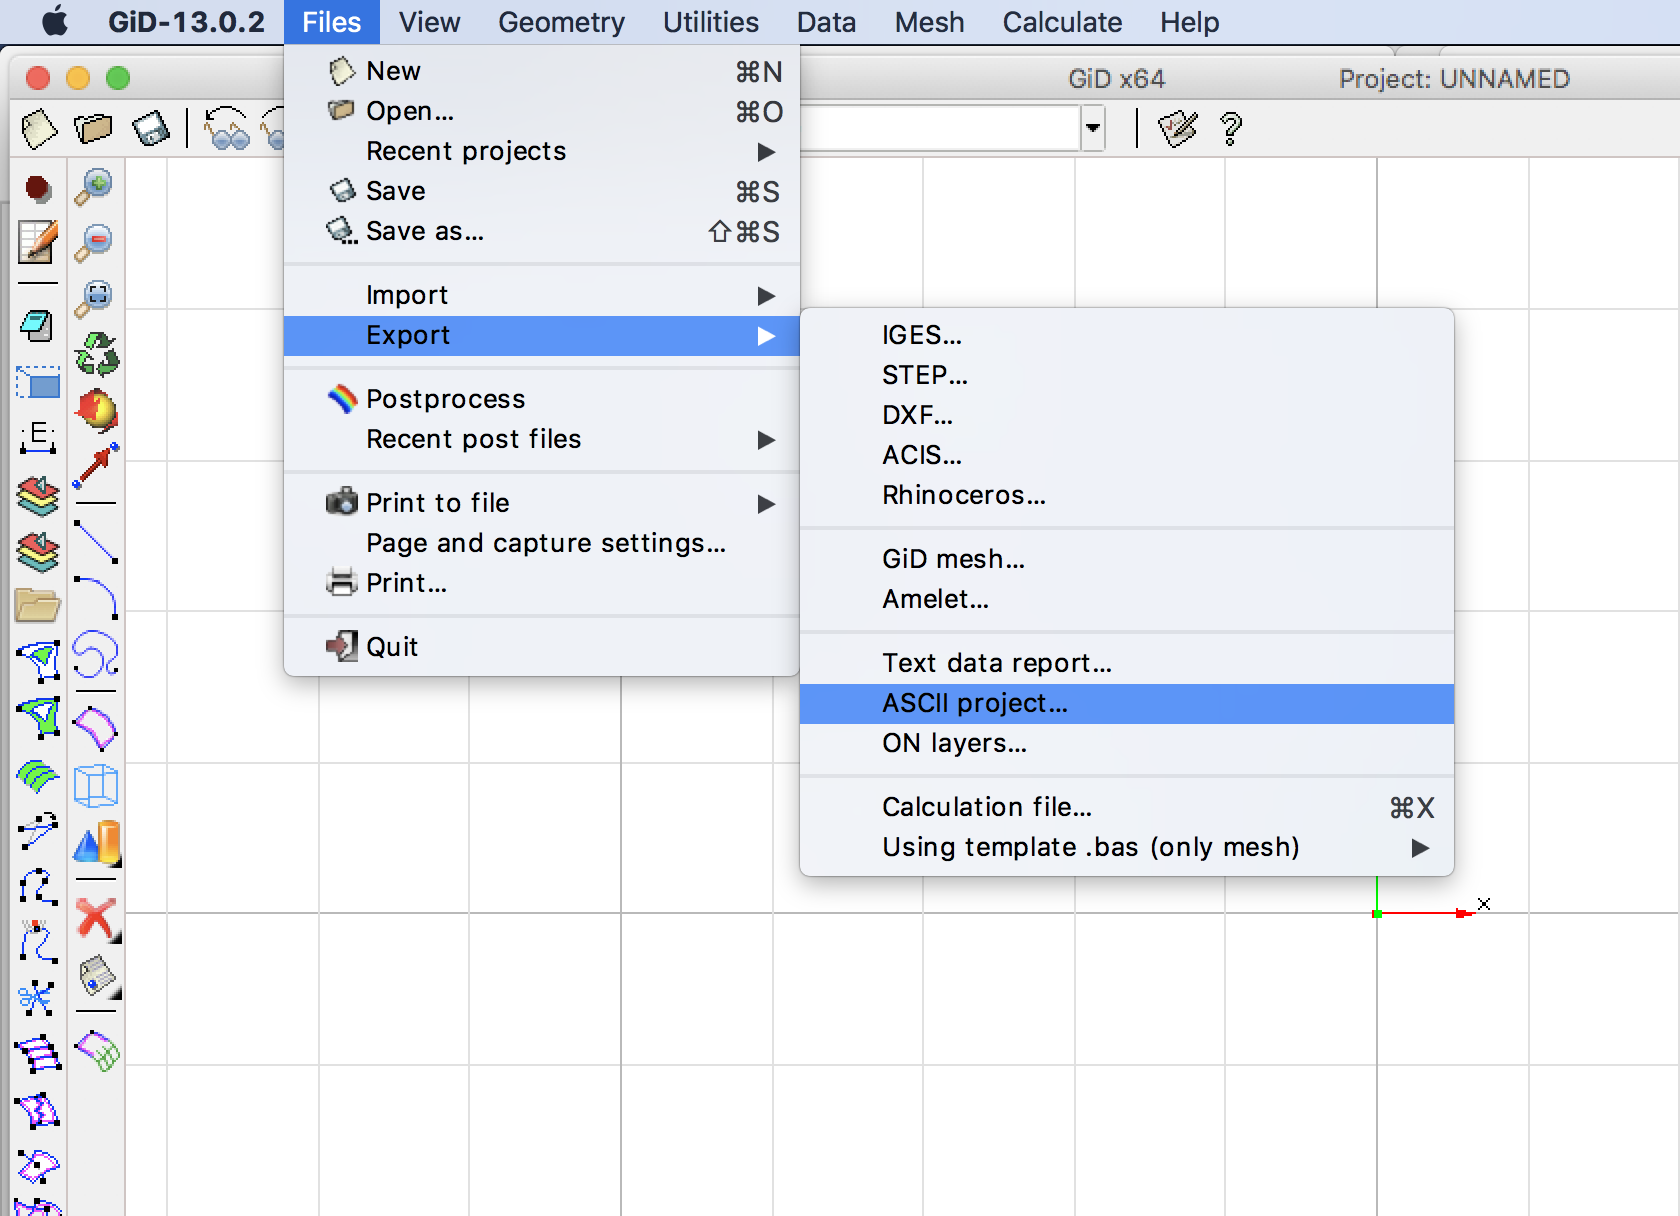
\includegraphics[width=3in]{GID_figure_4.png}%
\end{center}
\caption{}
\label{GID_figure_4}
\end{figure}

It will generate several files in a folder and the .msh file is the useful one for us.

\newpage
\section{Different Examples}





\subsection{Round\_2.msh (adaptive\_flag=0)}
Simple example withe smooth uniform geometry (figure \ref{Round_2} and \ref{Round_2_skeleton}). 

\begin{figure}[H]
\begin{center}
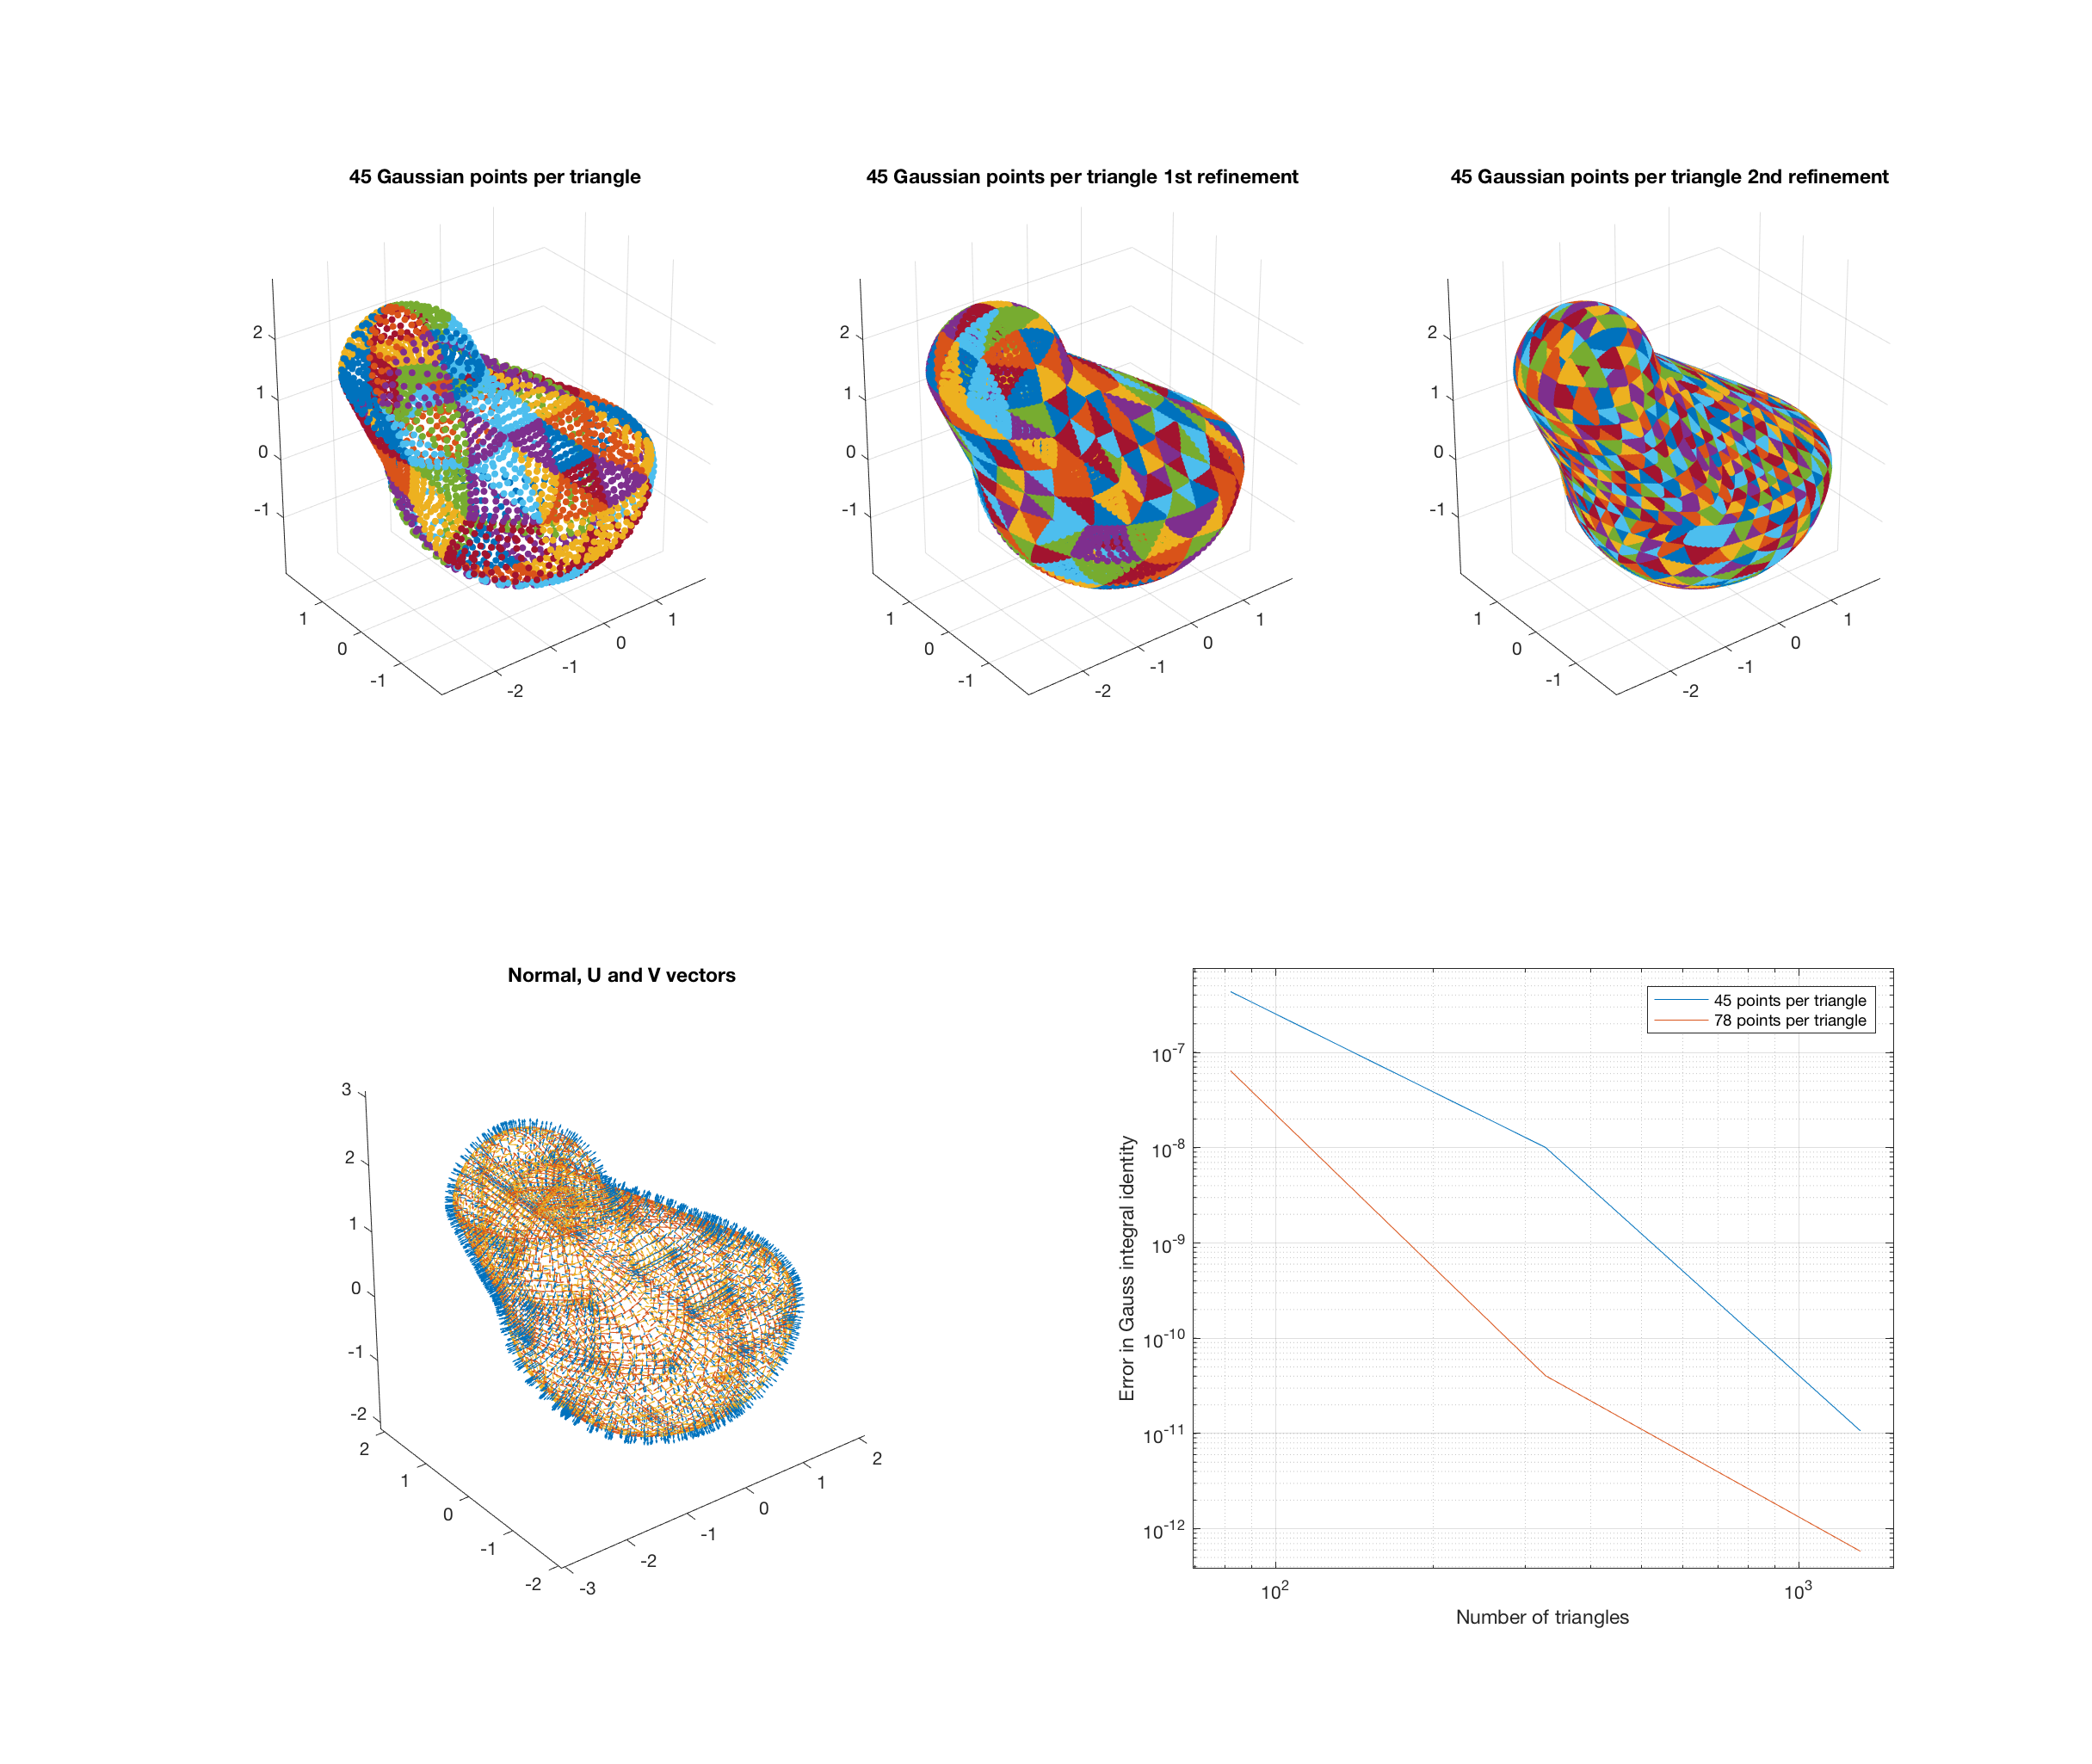
\includegraphics[width=6in]{Round_2.pdf}
\end{center}
\caption{The first row of figures show the refinement process with $n_{refinement}=0, n_{refinement}=1, n_{refinement}=2$ respectively.
The figure down-left shows the normal vector and two tangent orthogonal vectors U, V (all unitary) on each discretization point. The figure down-right shows the convergence obtained.}
\label{Round_2}
\end{figure}


\begin{figure}[H]
\begin{center}
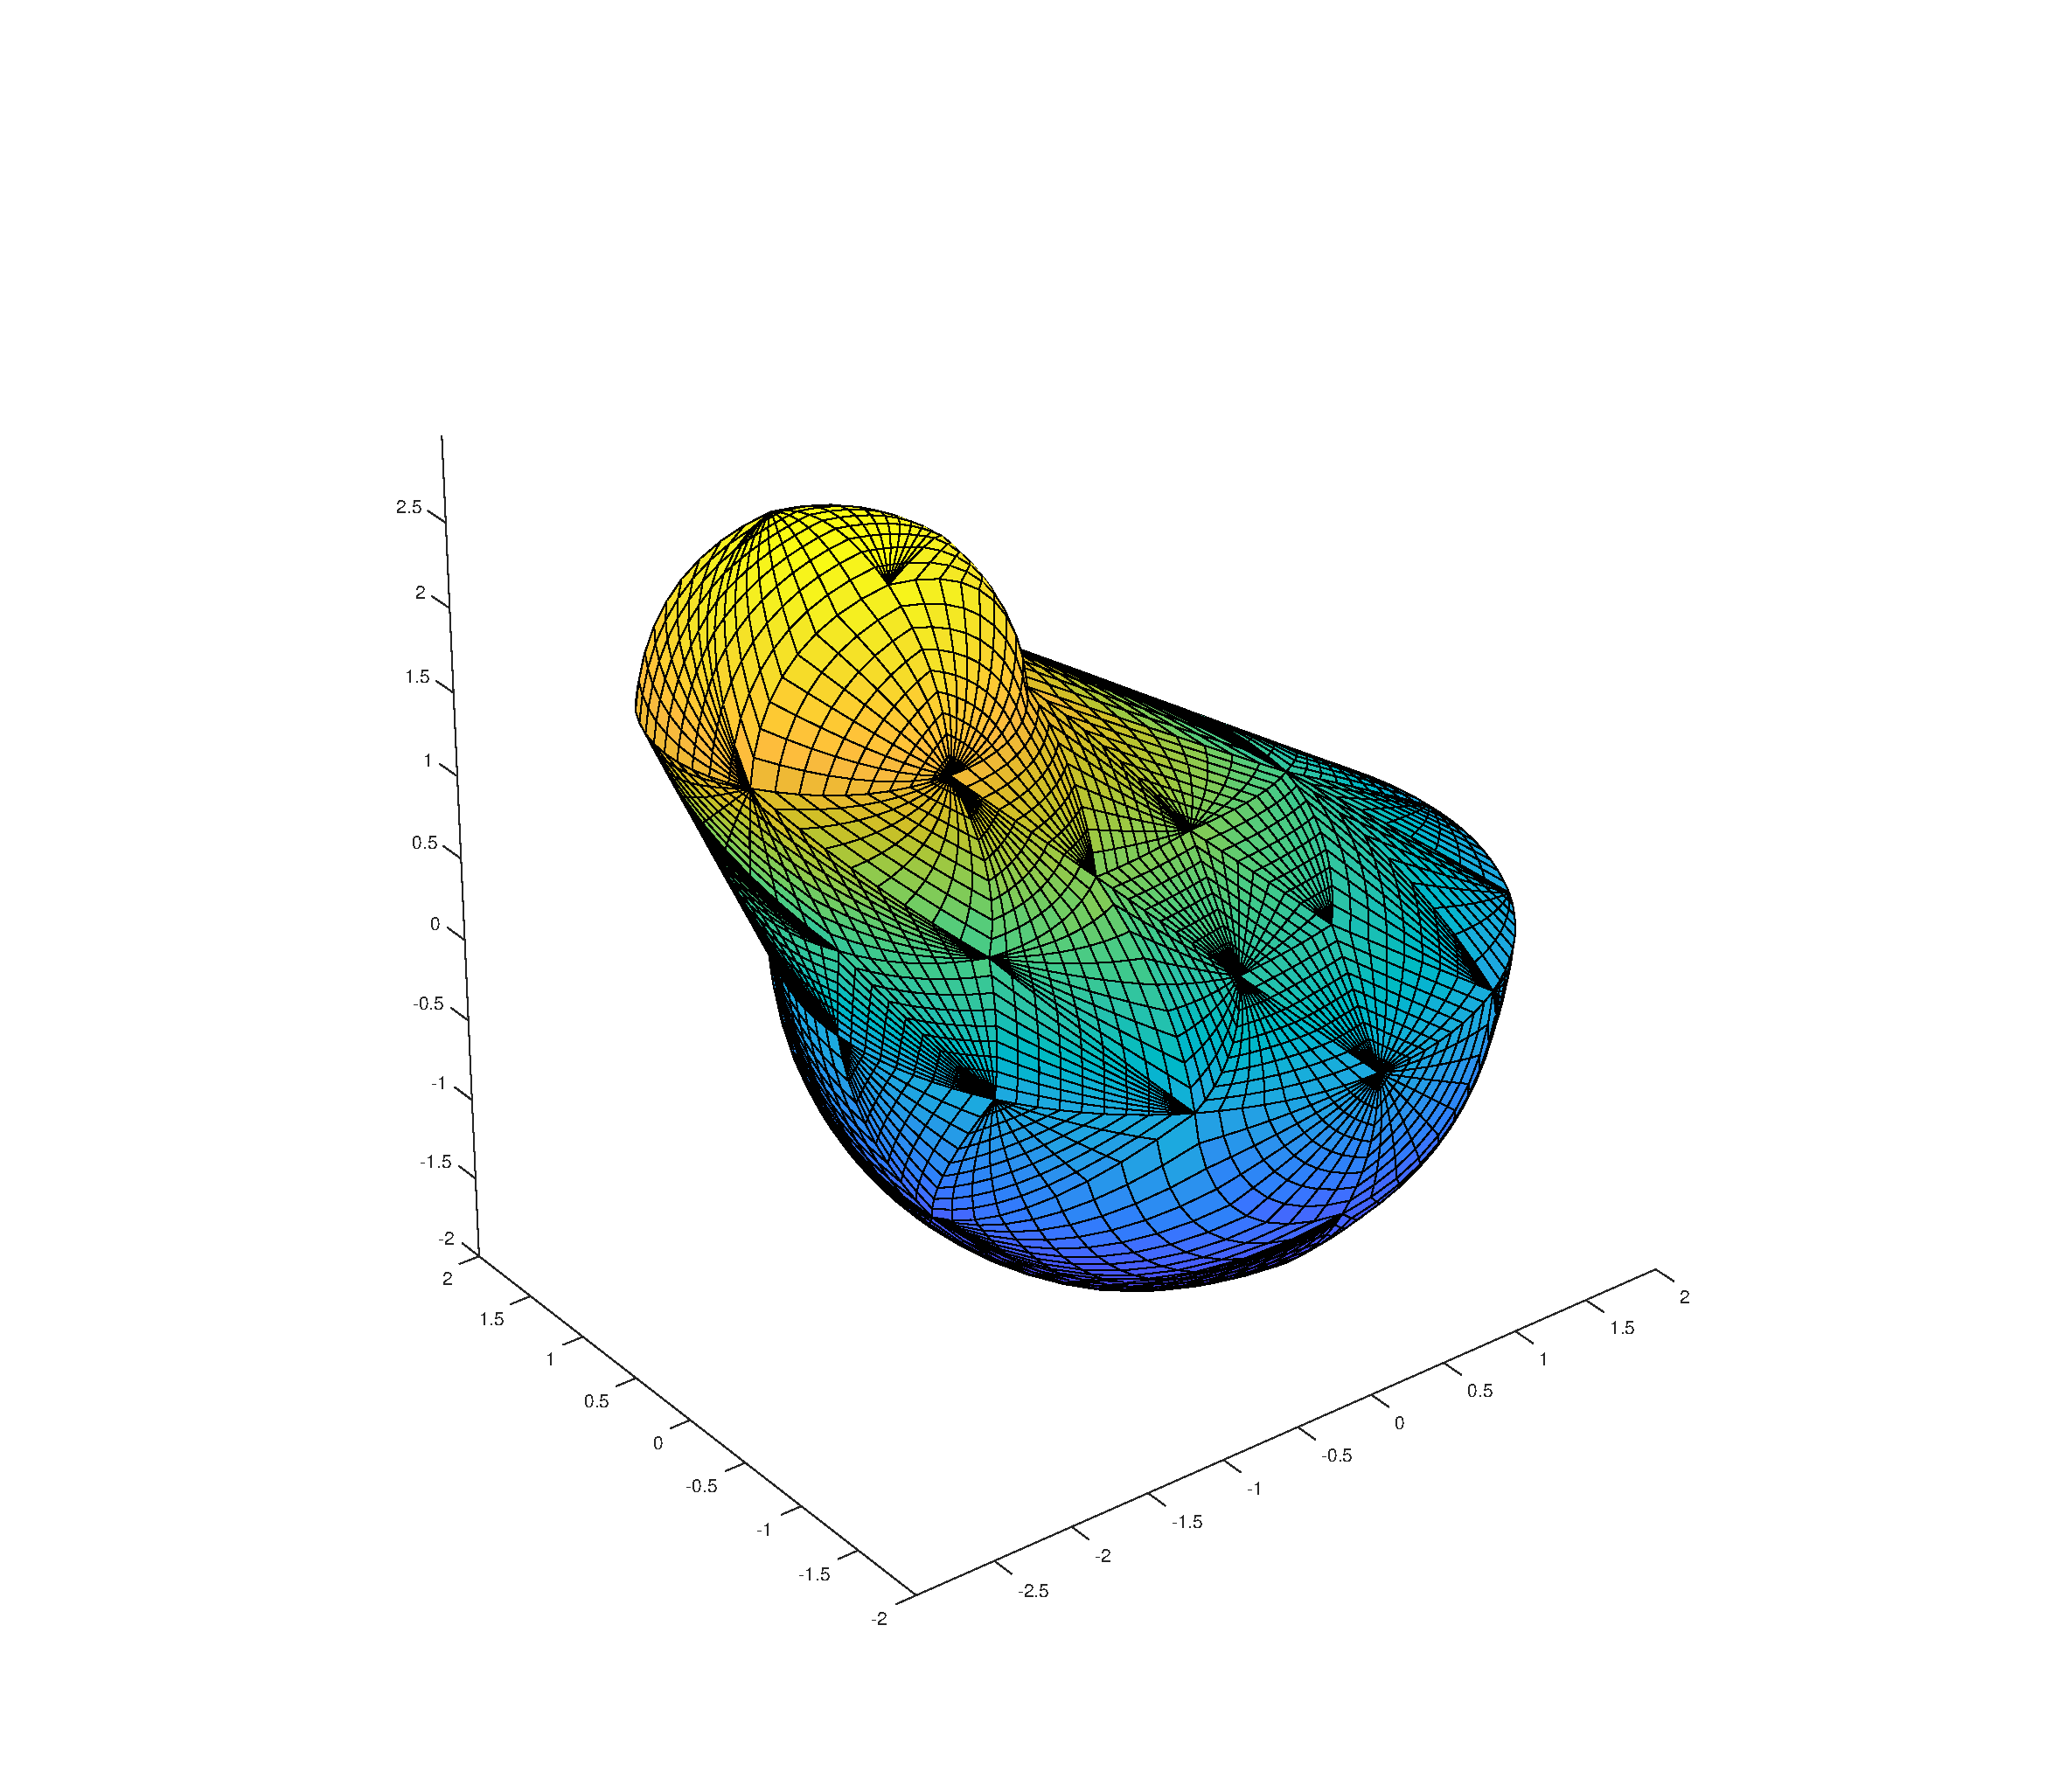
\includegraphics[width=6in]{Round_2_skeleton.pdf}
\end{center}
\caption{Round\_2.msh geometry. Skeleton based on quadratic triangles. The apparent distortion of the triangles is only present in this figure, not in the file (is a plot issue). The set of sources used for the FMM call are 78 Gauss nodes on each quadratic triangle}
\label{Round_2_skeleton}
\end{figure}






\newpage
\subsection{Round\_1.msh (adaptive\_flag=0)}
Simple example withe smooth uniform geometry (figure \ref{Round_1} and \ref{Round_1_skeleton}). 

\begin{figure}[H]
\begin{center}
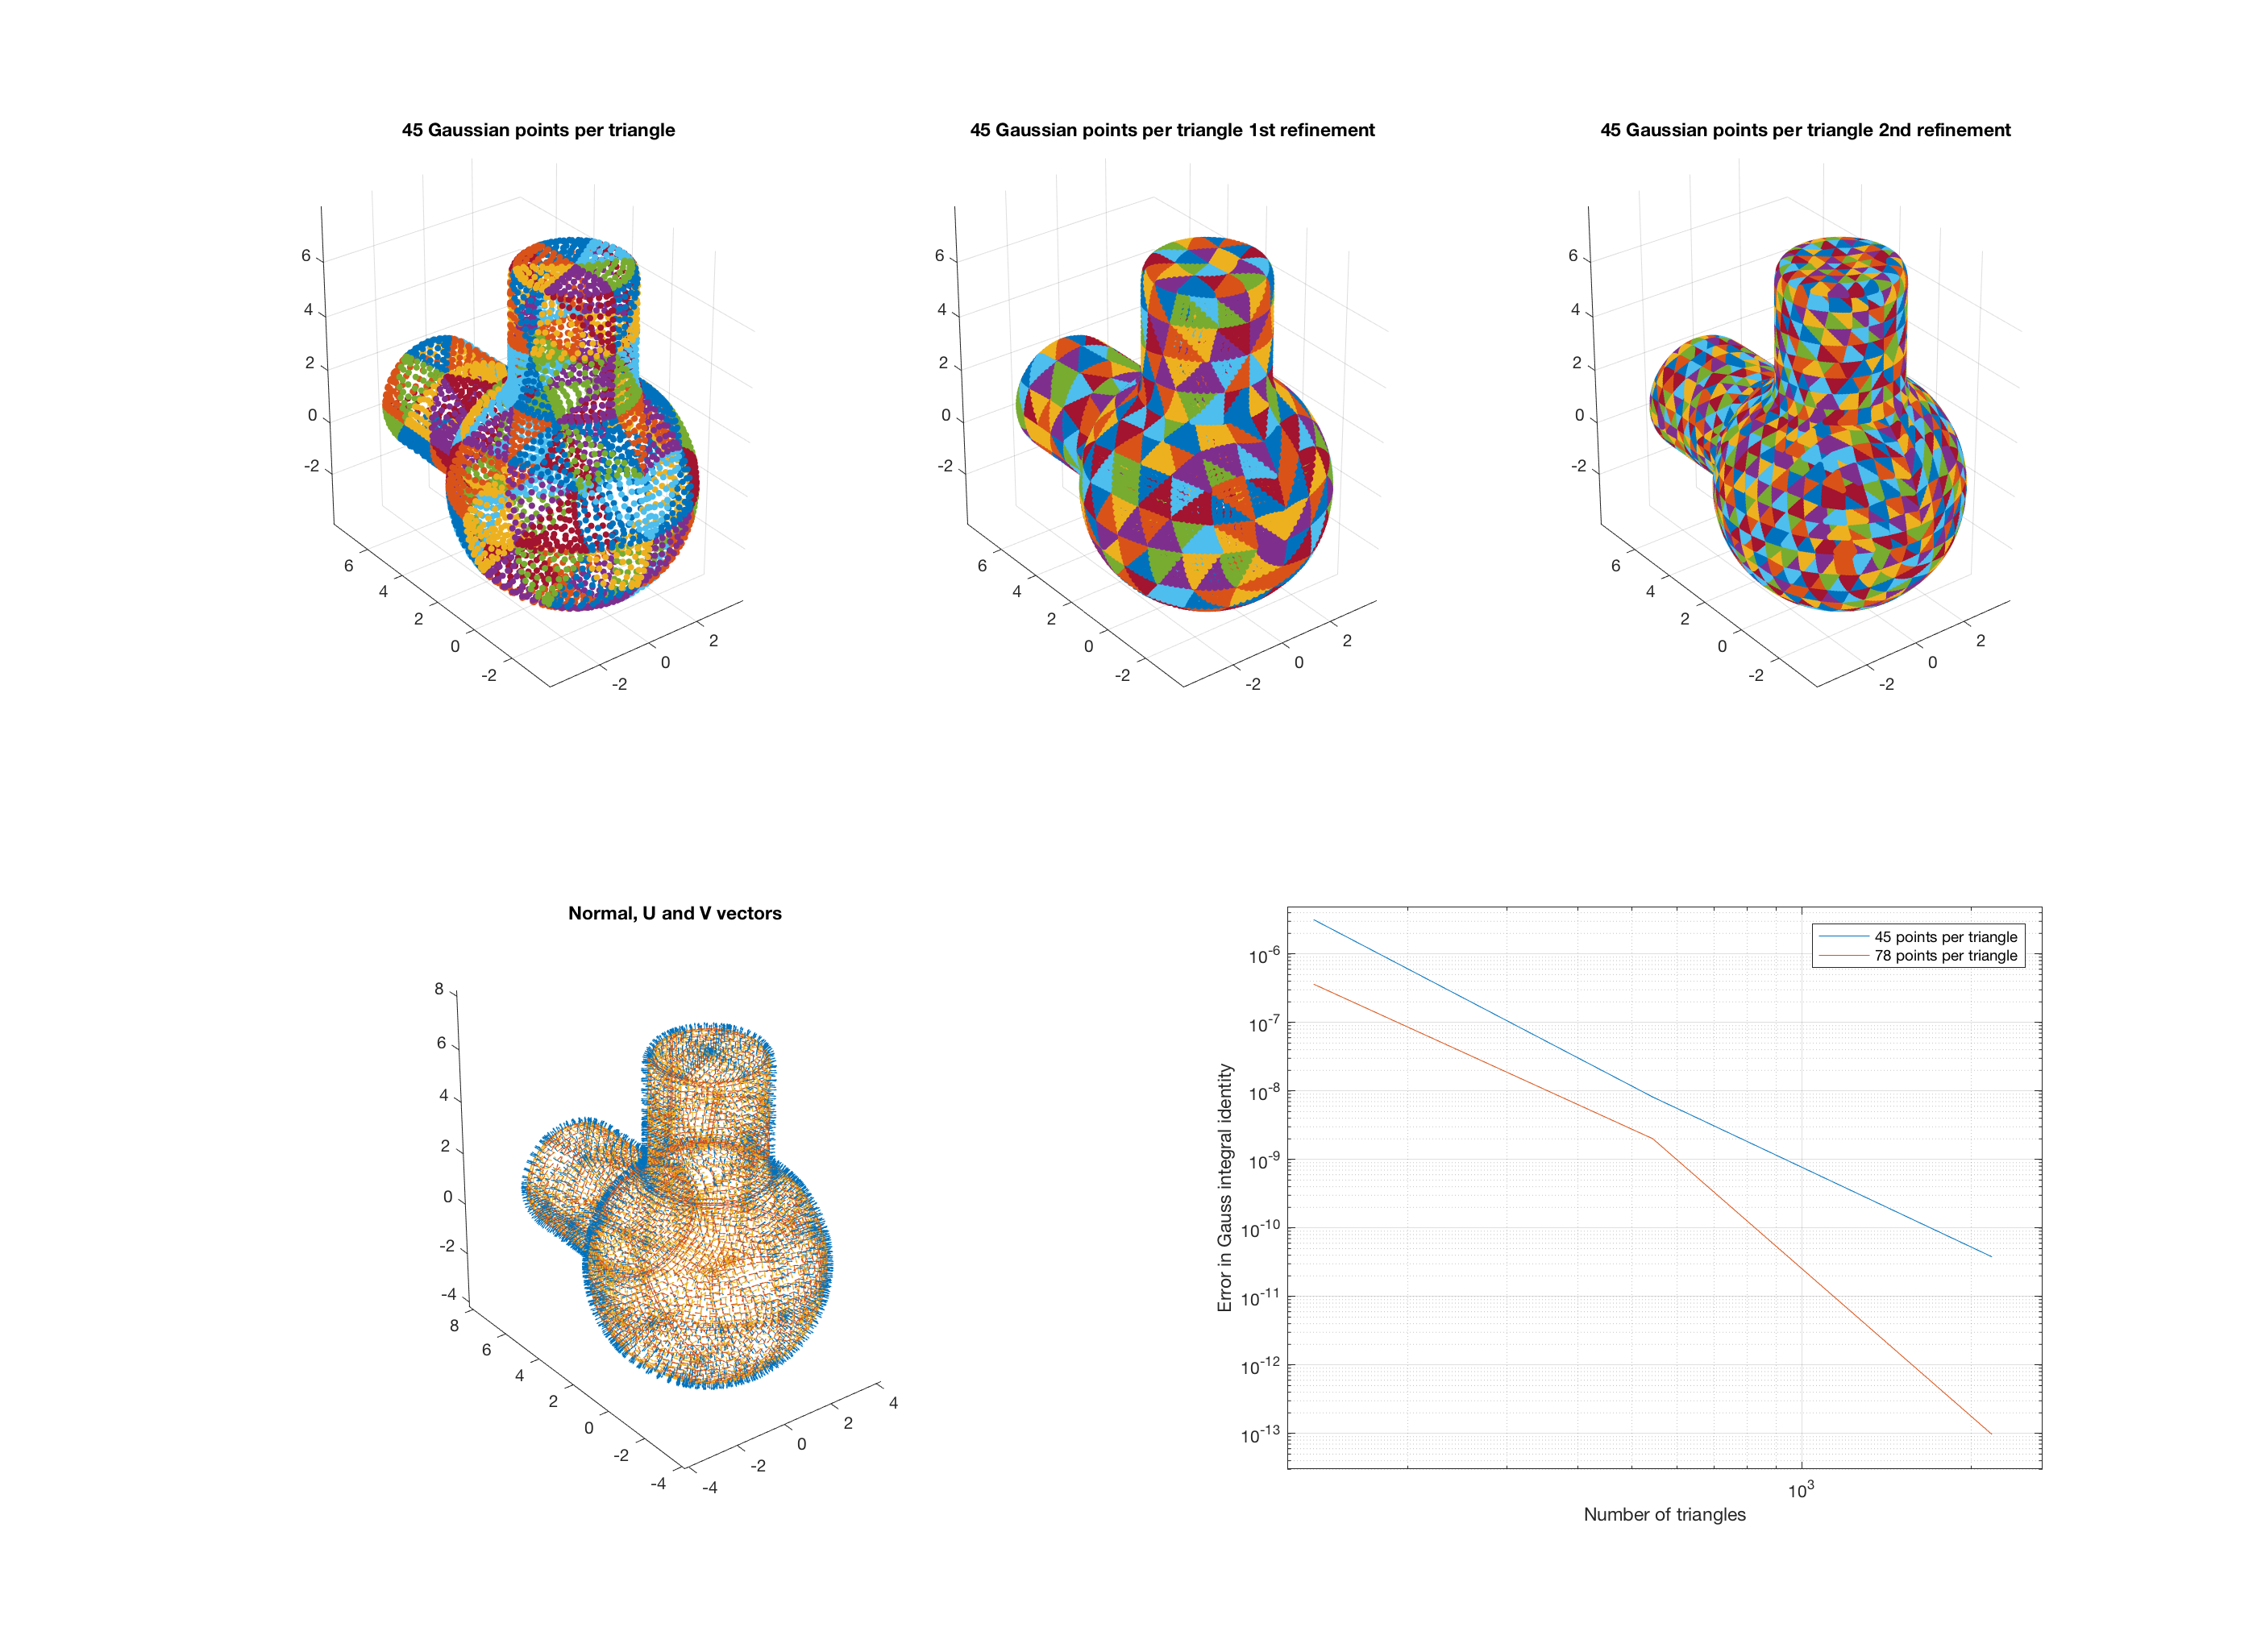
\includegraphics[width=6in]{Round_1.pdf}
\end{center}
\caption{The first row of figures show the refinement process with $n_{refinement}=0, n_{refinement}=1, n_{refinement}=2$ respectively.
The figure down-left shows the normal vector and two tangent orthogonal vectors U, V (all unitary) on each discretization point. The figure down-right shows the convergence obtained.}
\label{Round_1}
\end{figure}


\begin{figure}[H]
\begin{center}
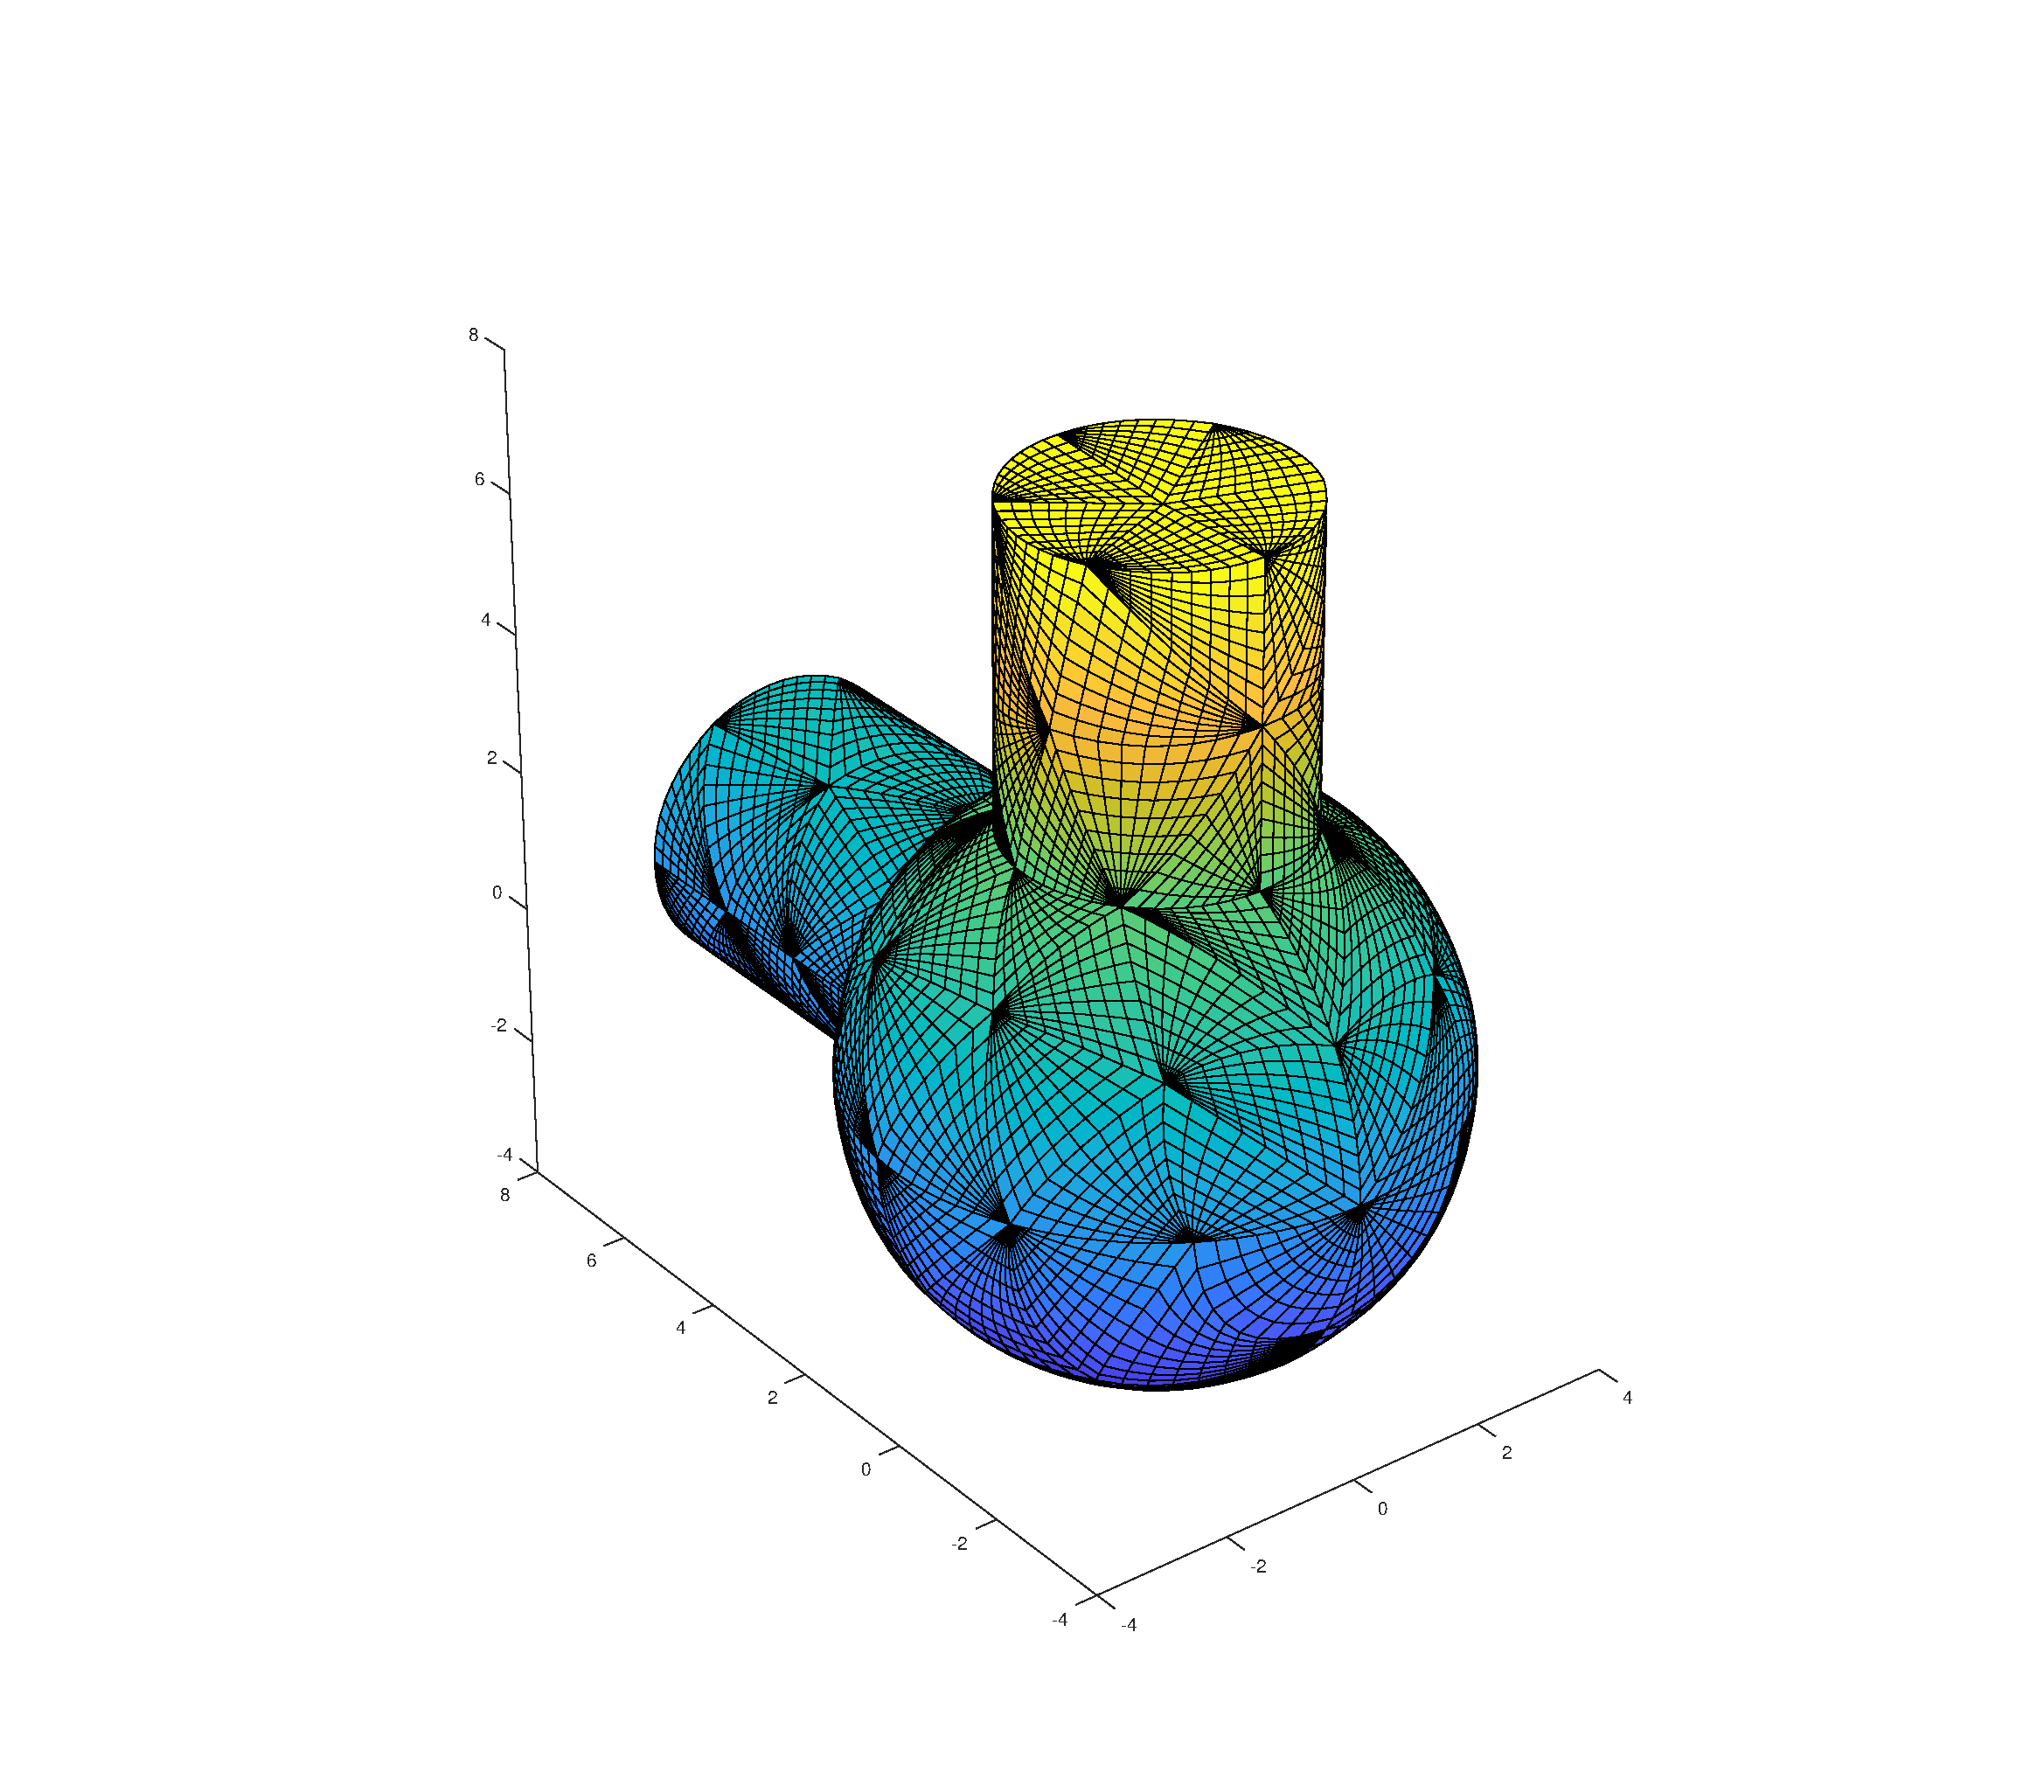
\includegraphics[width=6in]{Round_1_skeleton.pdf}
\end{center}
\caption{Round\_1.msh geometry. Skeleton based on quadratic triangles. The apparent distortion of the triangles is only present in this figure, not in the file (is a plot issue). The set of sources used for the FMM call are 78 Gauss nodes on each quadratic triangle}
\label{Round_1_skeleton}
\end{figure}






\newpage
\subsection{Cube\_substraction.msh (adaptive\_flag=0)}
REMARK: We see a saturation in the accuracy at 12 digits (figure \ref{cube_substraction} down right) because of the Newton threshold and other FMM threshold (iprec=3).

\begin{figure}[H]
\begin{center}
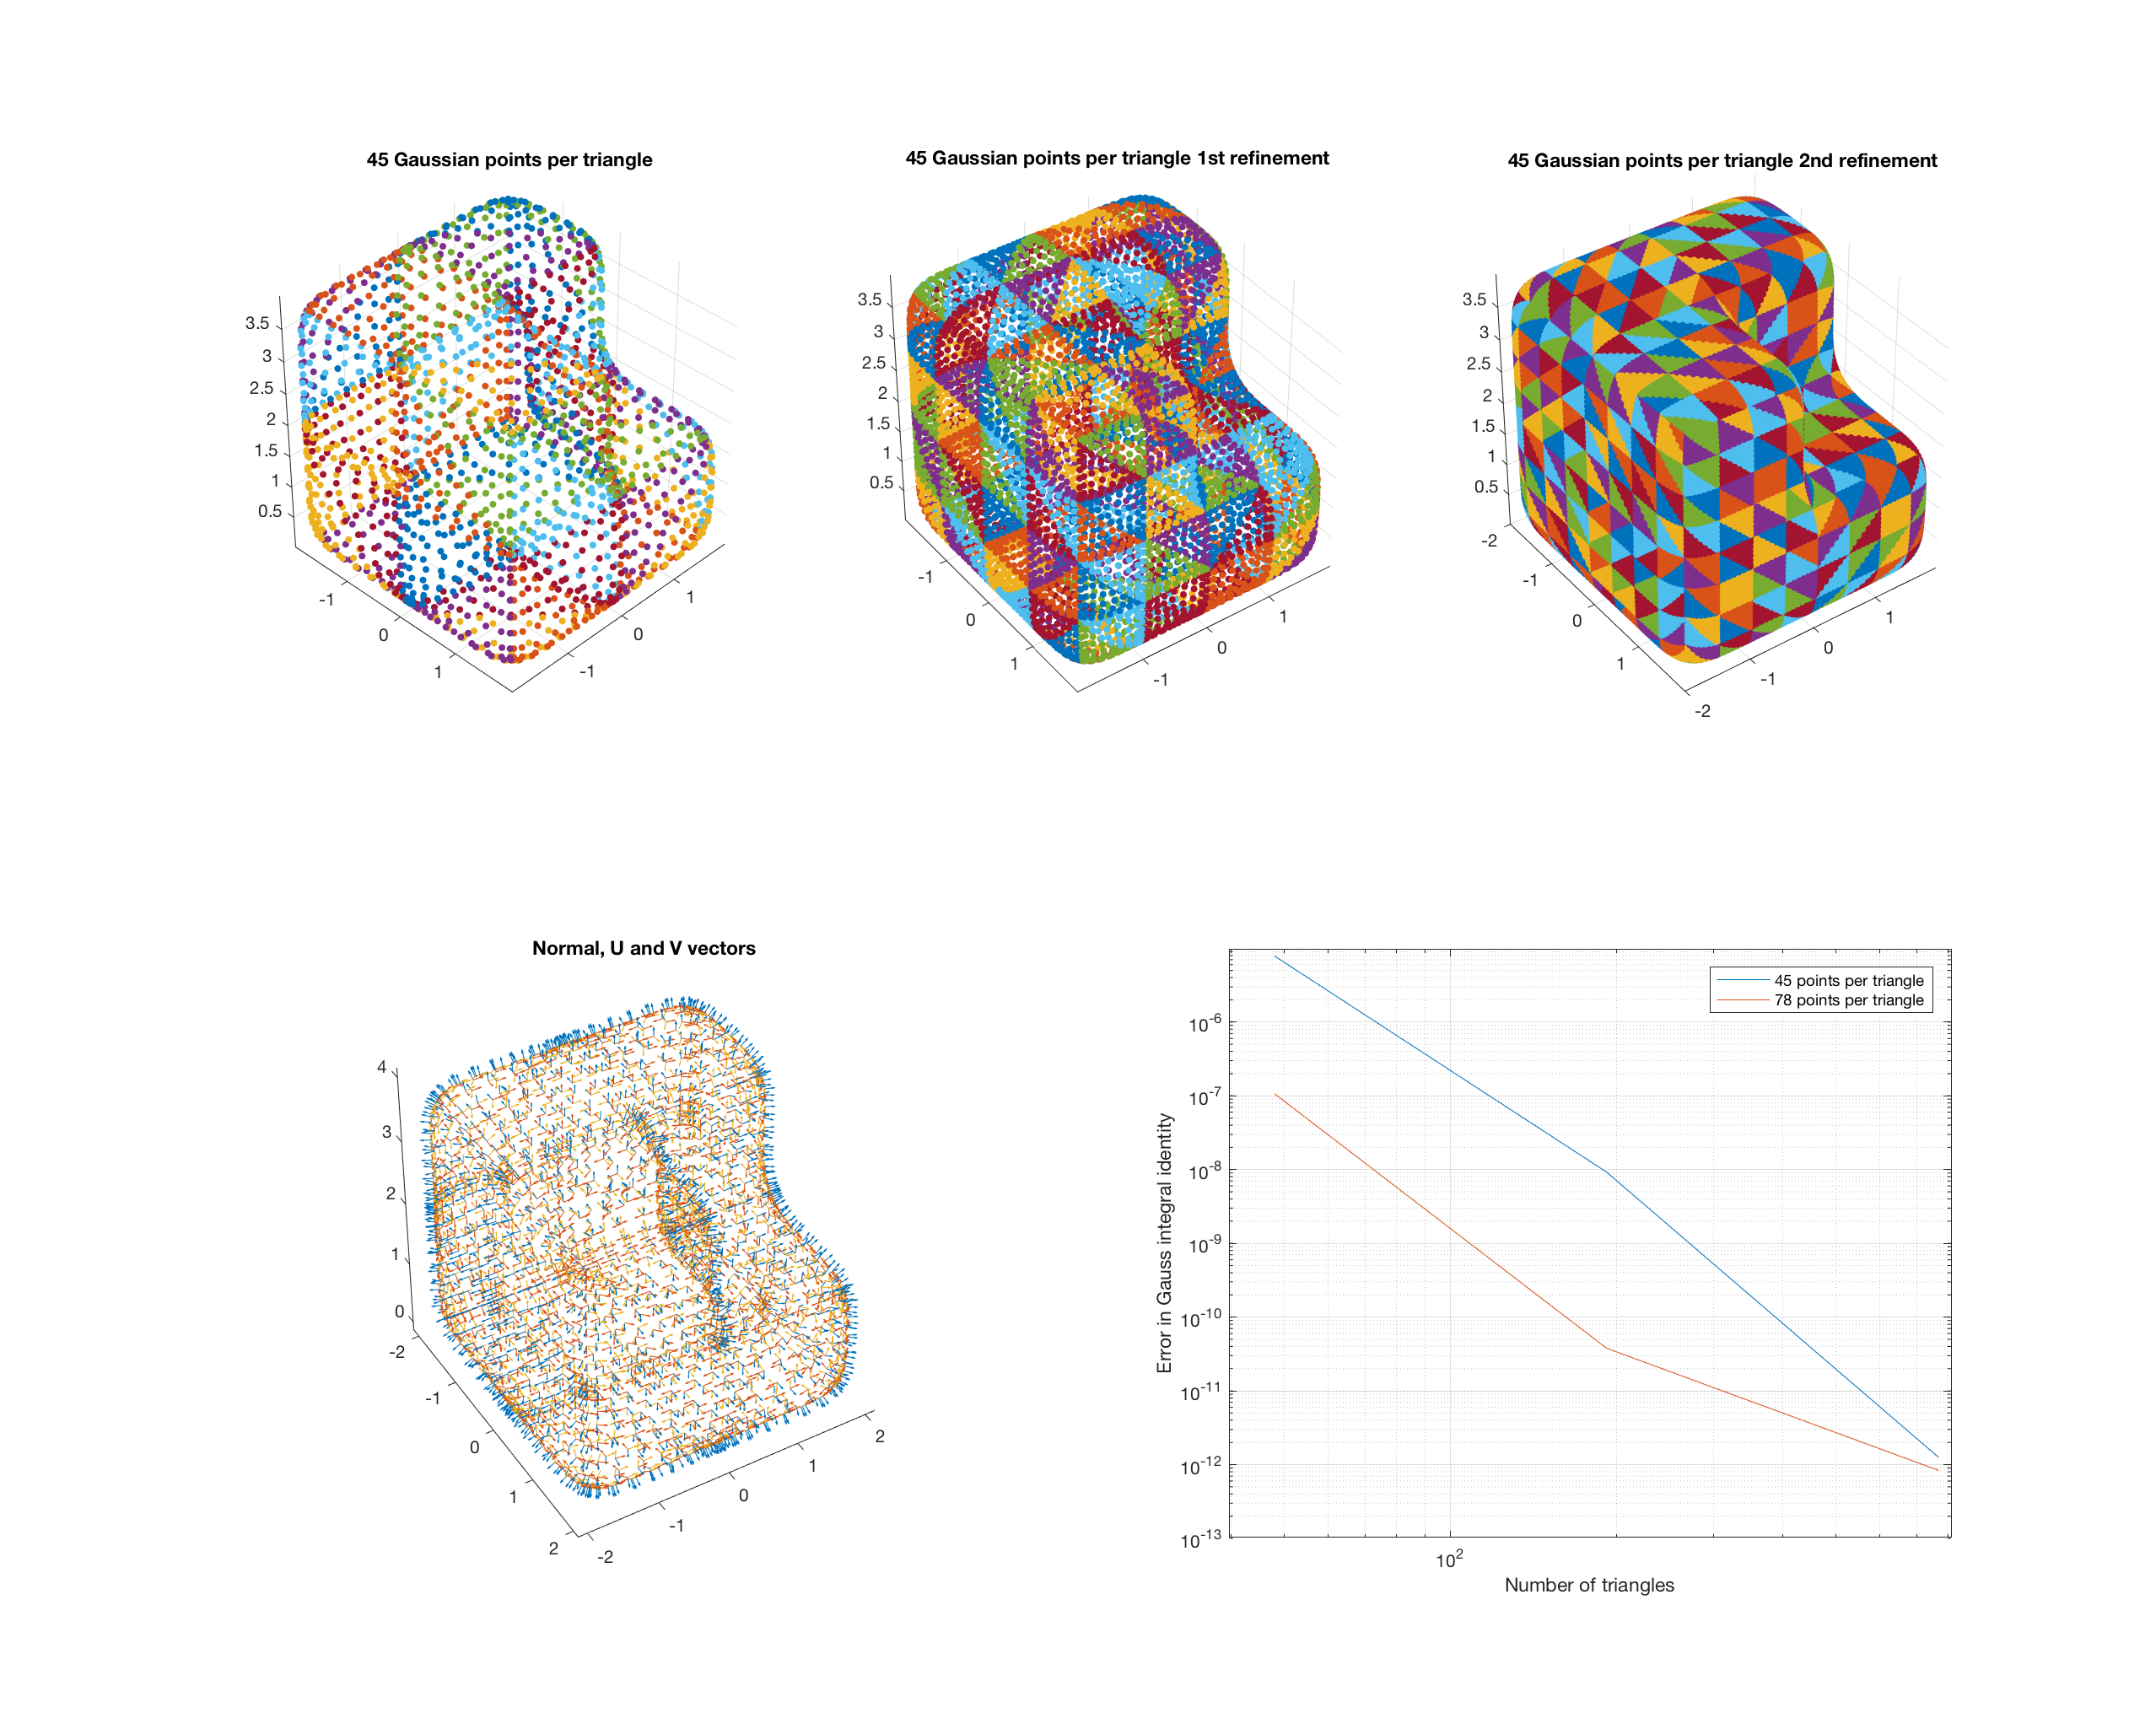
\includegraphics[width=6in]{cube_substraction.pdf}
\end{center}
\caption{The first row of figures show the refinement process with $n_{refinement}=0, n_{refinement}=1, n_{refinement}=2$ respectively.
The figure down left shows the normal vector and two tangent orthogonal vectors U, V (all unitary) on each discretization point. The figure down right shows the convergence obtained. We see a saturation in the accuracy at 12 digits because of the Newton threshold and other FMM threshold (iprec=3)}
\label{cube_substraction}
\end{figure}


\begin{figure}[H]
\begin{center}
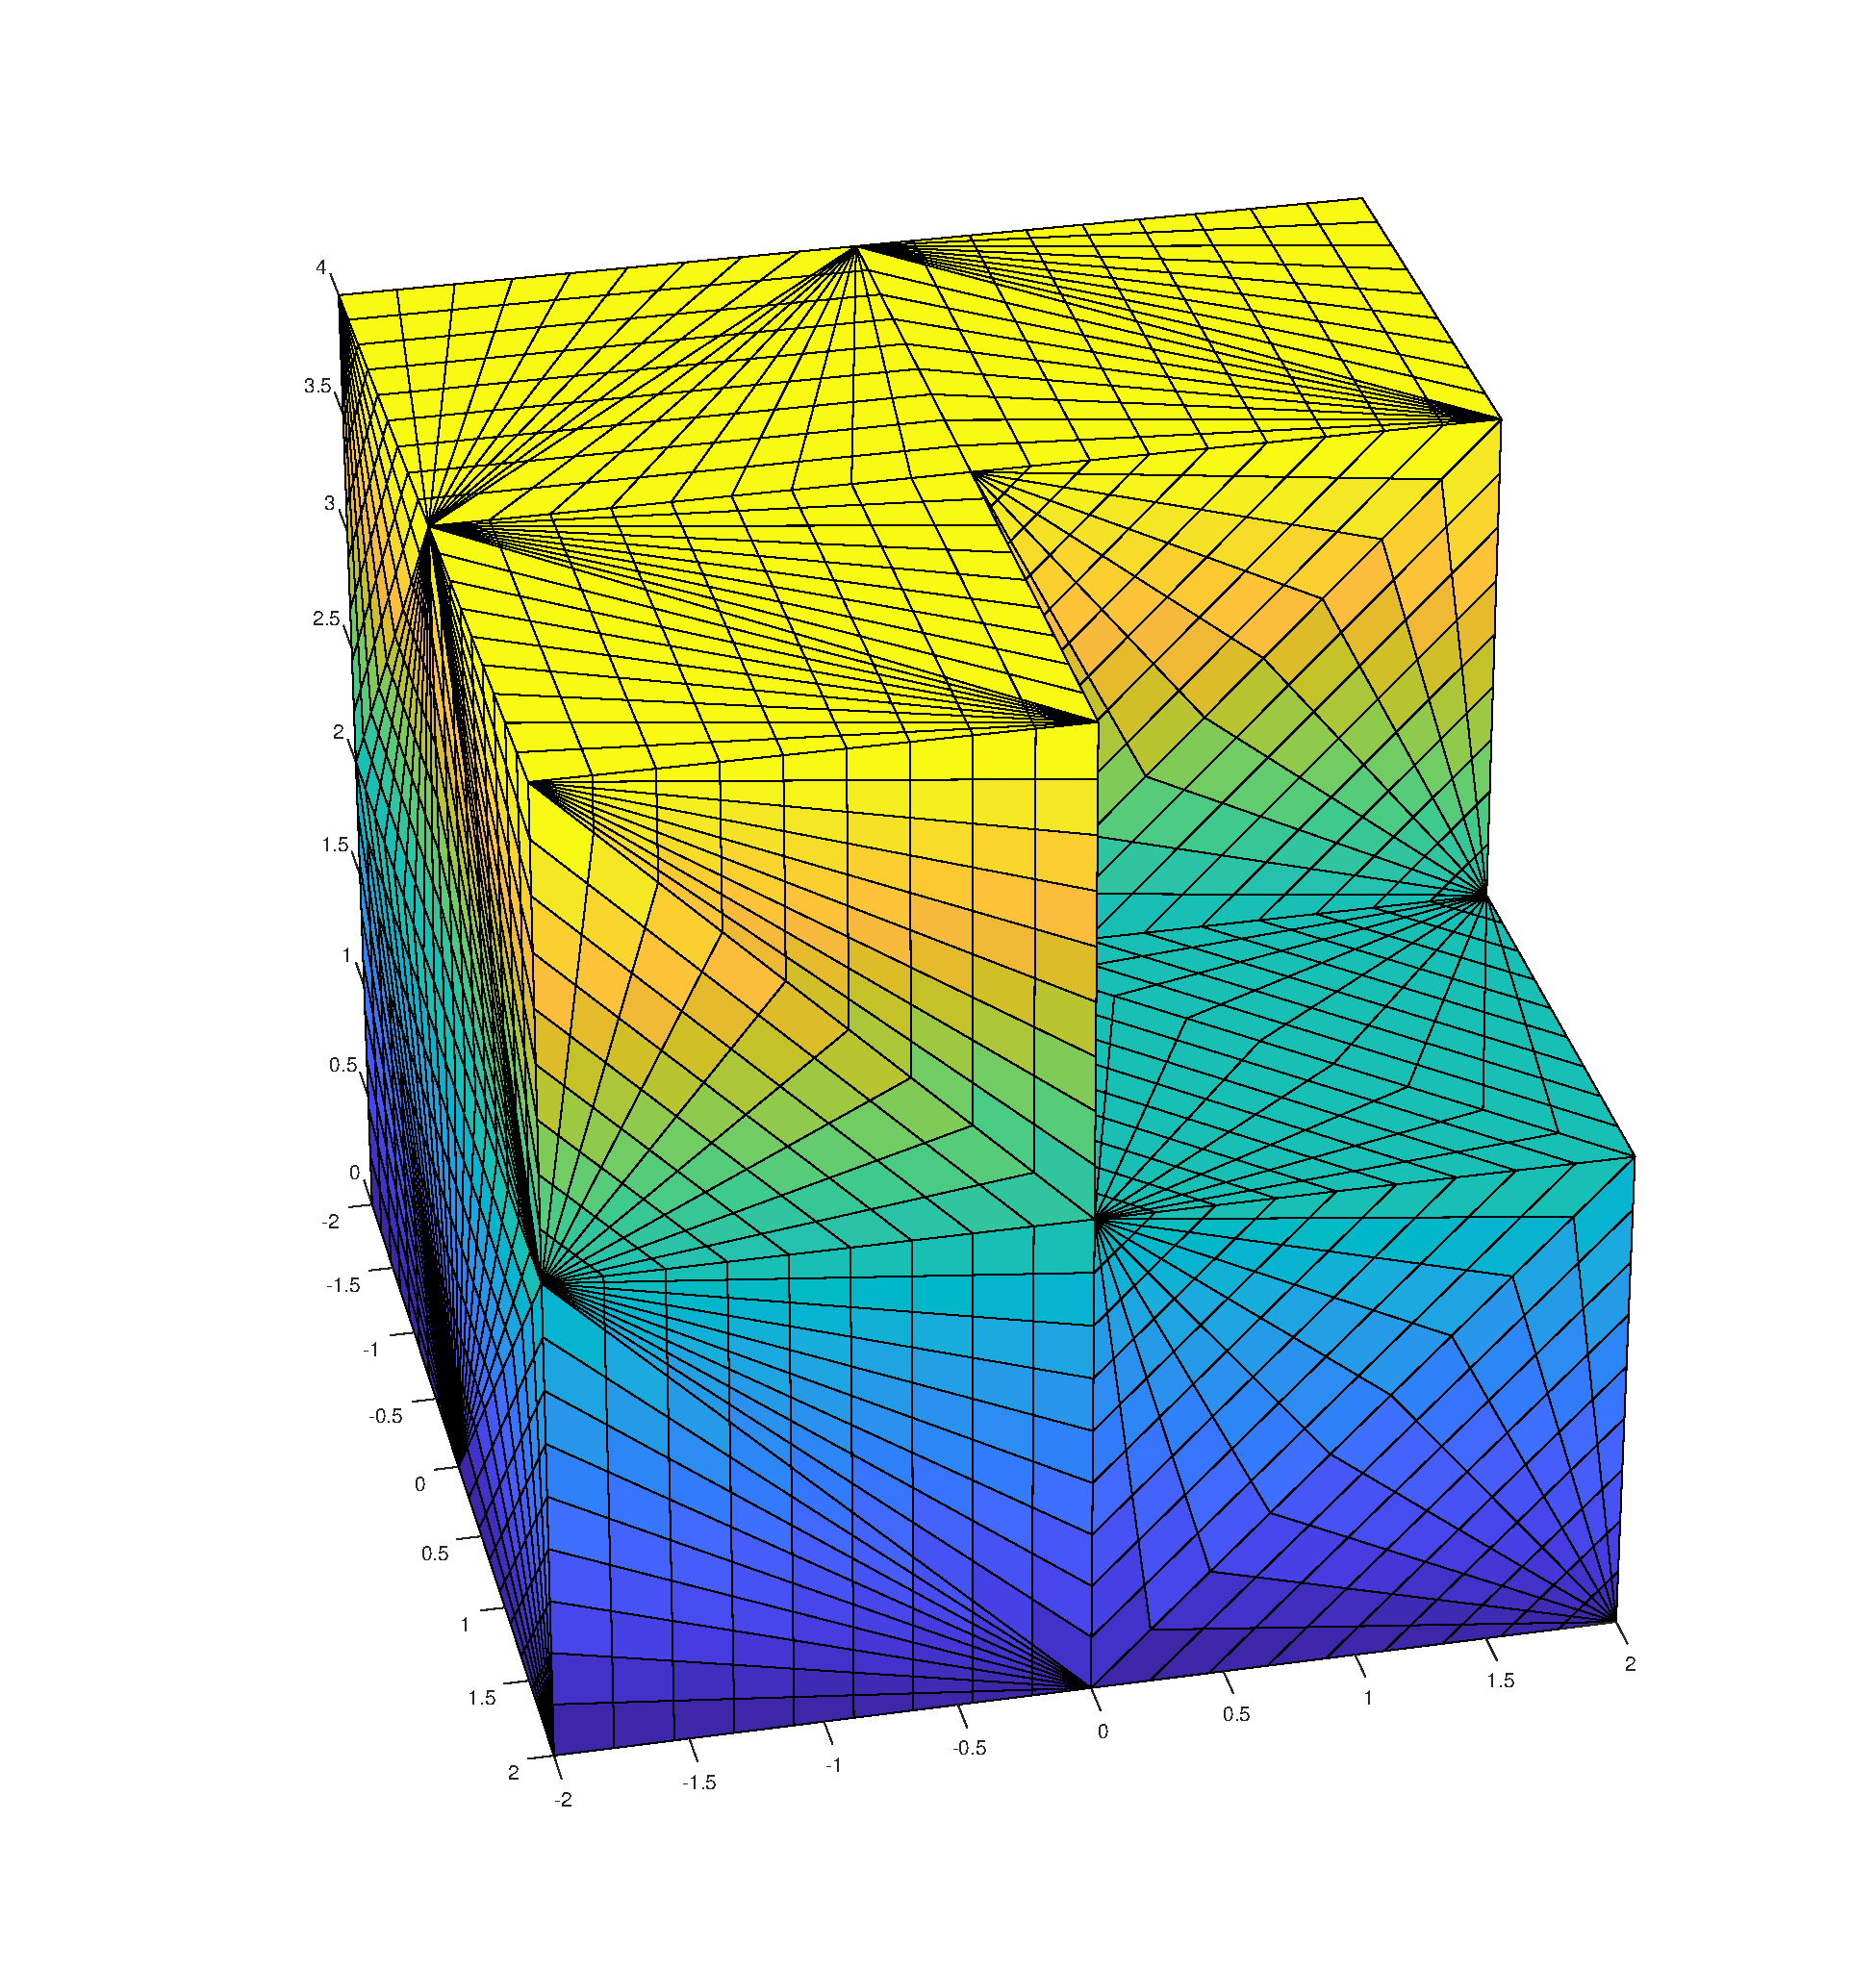
\includegraphics[width=6in]{cube_substraction_skeleton.pdf}
\end{center}
\caption{cube\_substraction.msh geometry. Skeleton based on quadratic triangles. The apparent distortion of the triangles is only present in this figure, not in the file (is a plot issue). The set of sources used for the FMM call are 78 Gauss nodes on each quadratic triangle}
\label{cube_substraction_skeleton}
\end{figure}













\newpage
\subsection{esfera\_esfera.msh (adaptive\_flag=0)}
Simple example of a spherical geometry with a spherical cavity (figure \ref{esfera_esfera} and \ref{esfera_esfera_skeleton}).

\begin{figure}[H]
\begin{center}
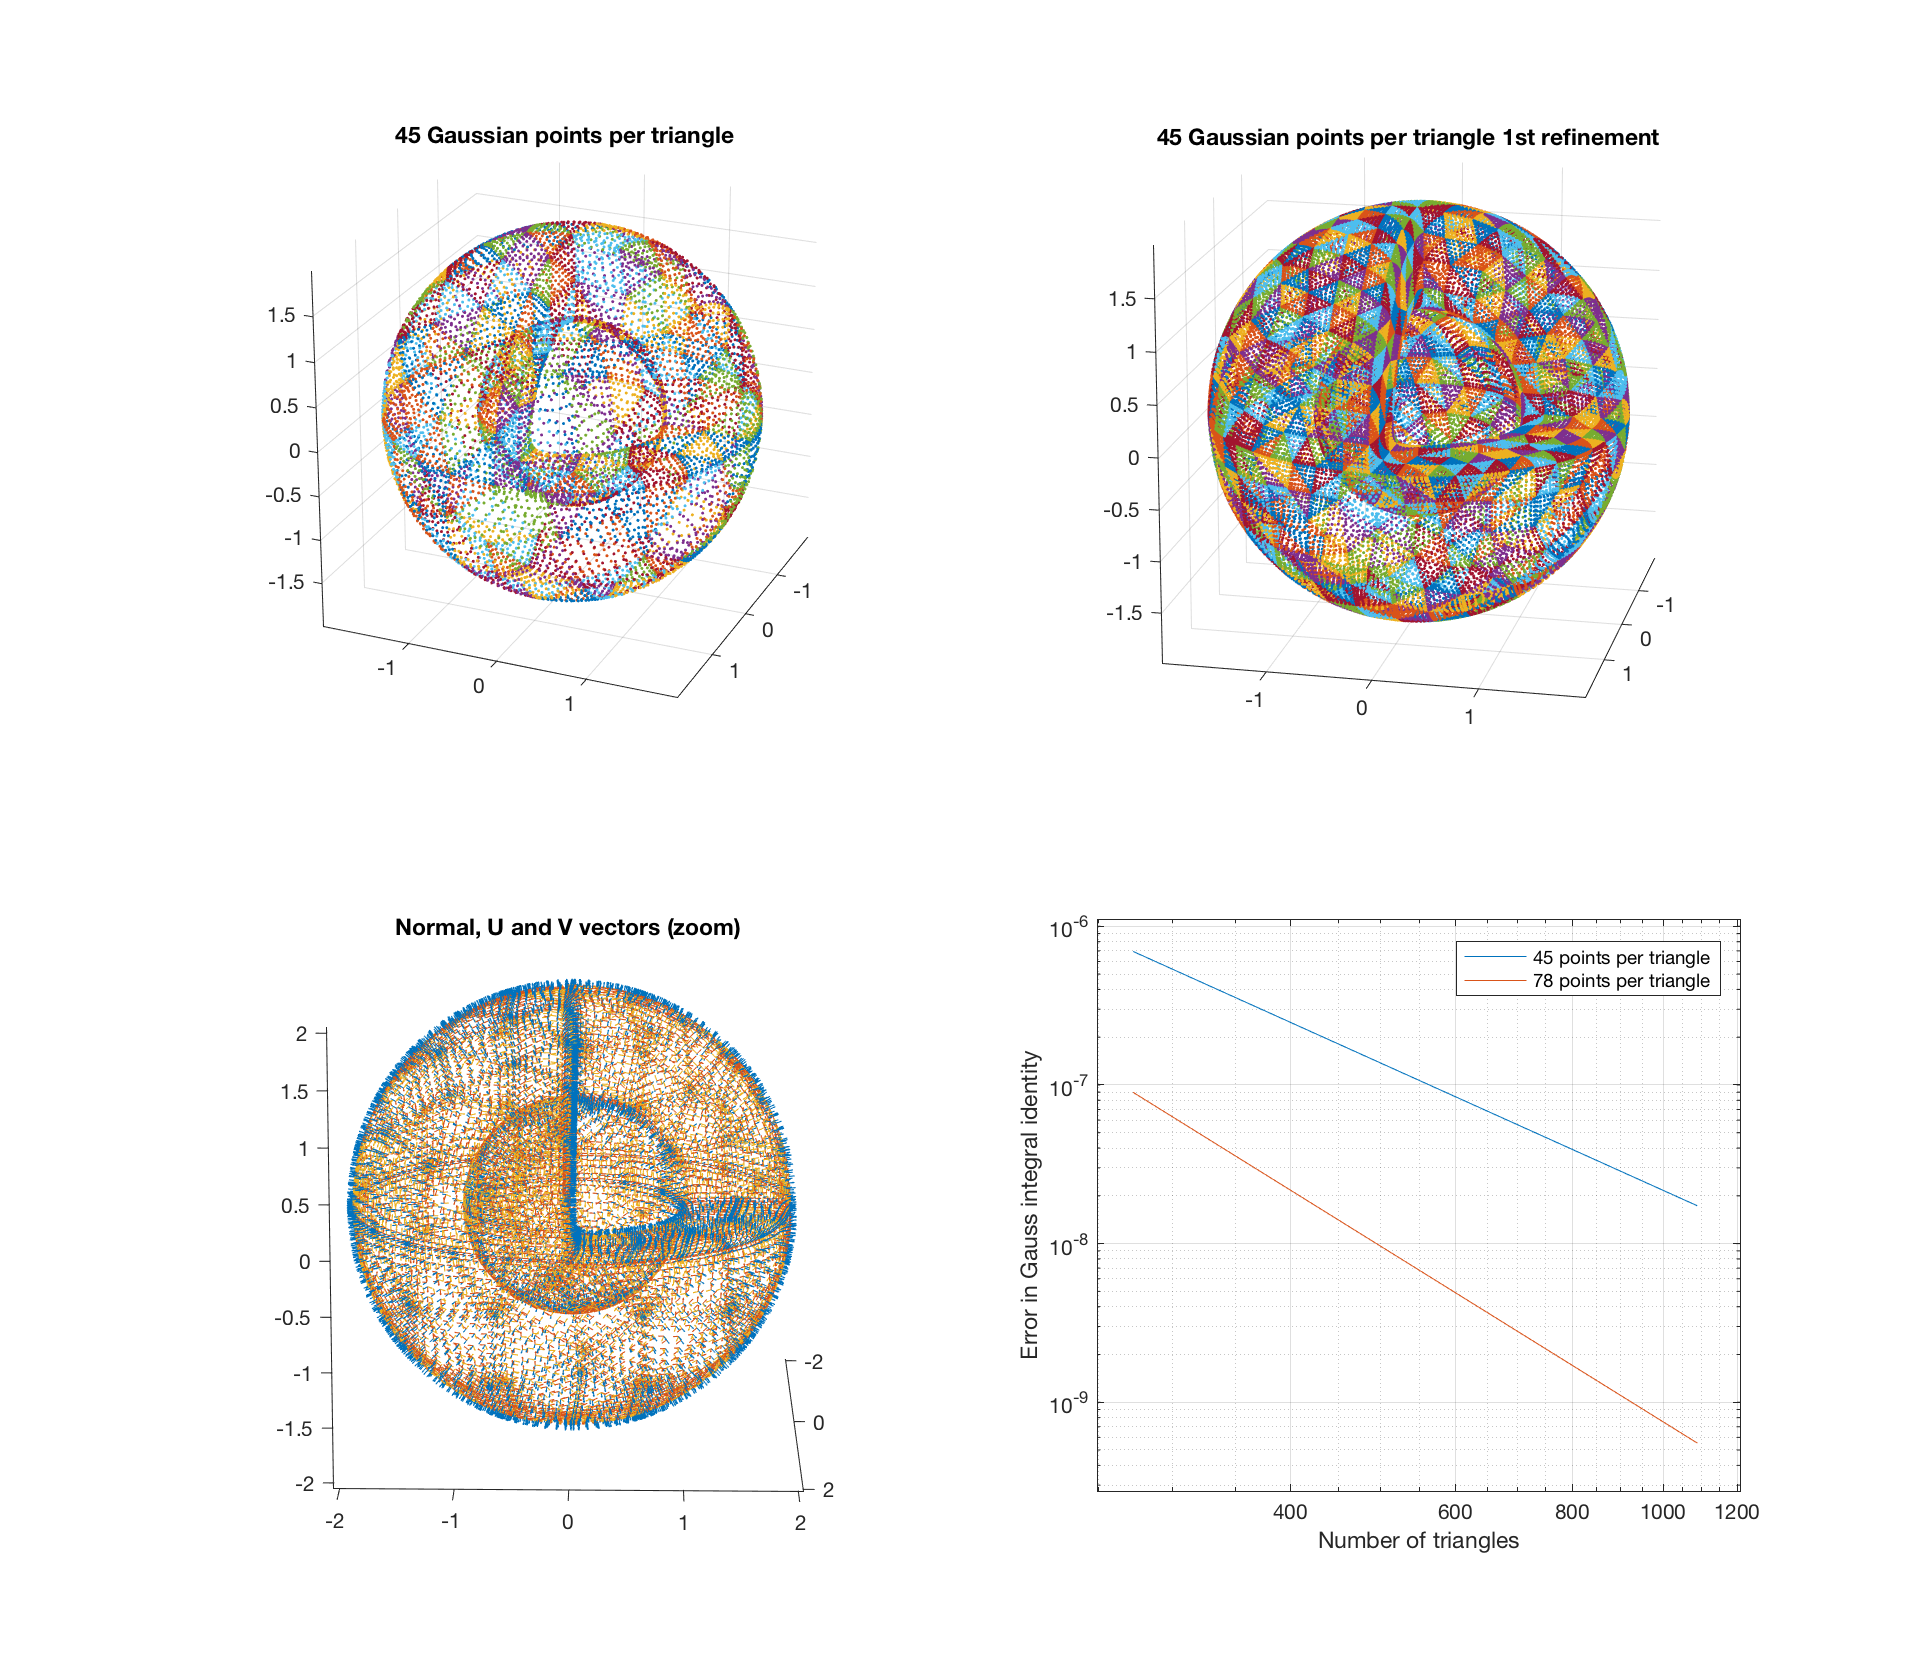
\includegraphics[width=6in]{esfera_esfera.pdf}
\end{center}
\caption{The first row of figures show the refinement process with $n_{refinement}=0, n_{refinement}=1$ respectively.
The figure down left shows the normal vector and two tangent orthogonal vectors U, V (all unitary) on each discretization point. The figure down right shows the convergence obtained. We can see the method working on simple geometries with cavities}
\label{esfera_esfera}
\end{figure}


\begin{figure}[H]
\begin{center}
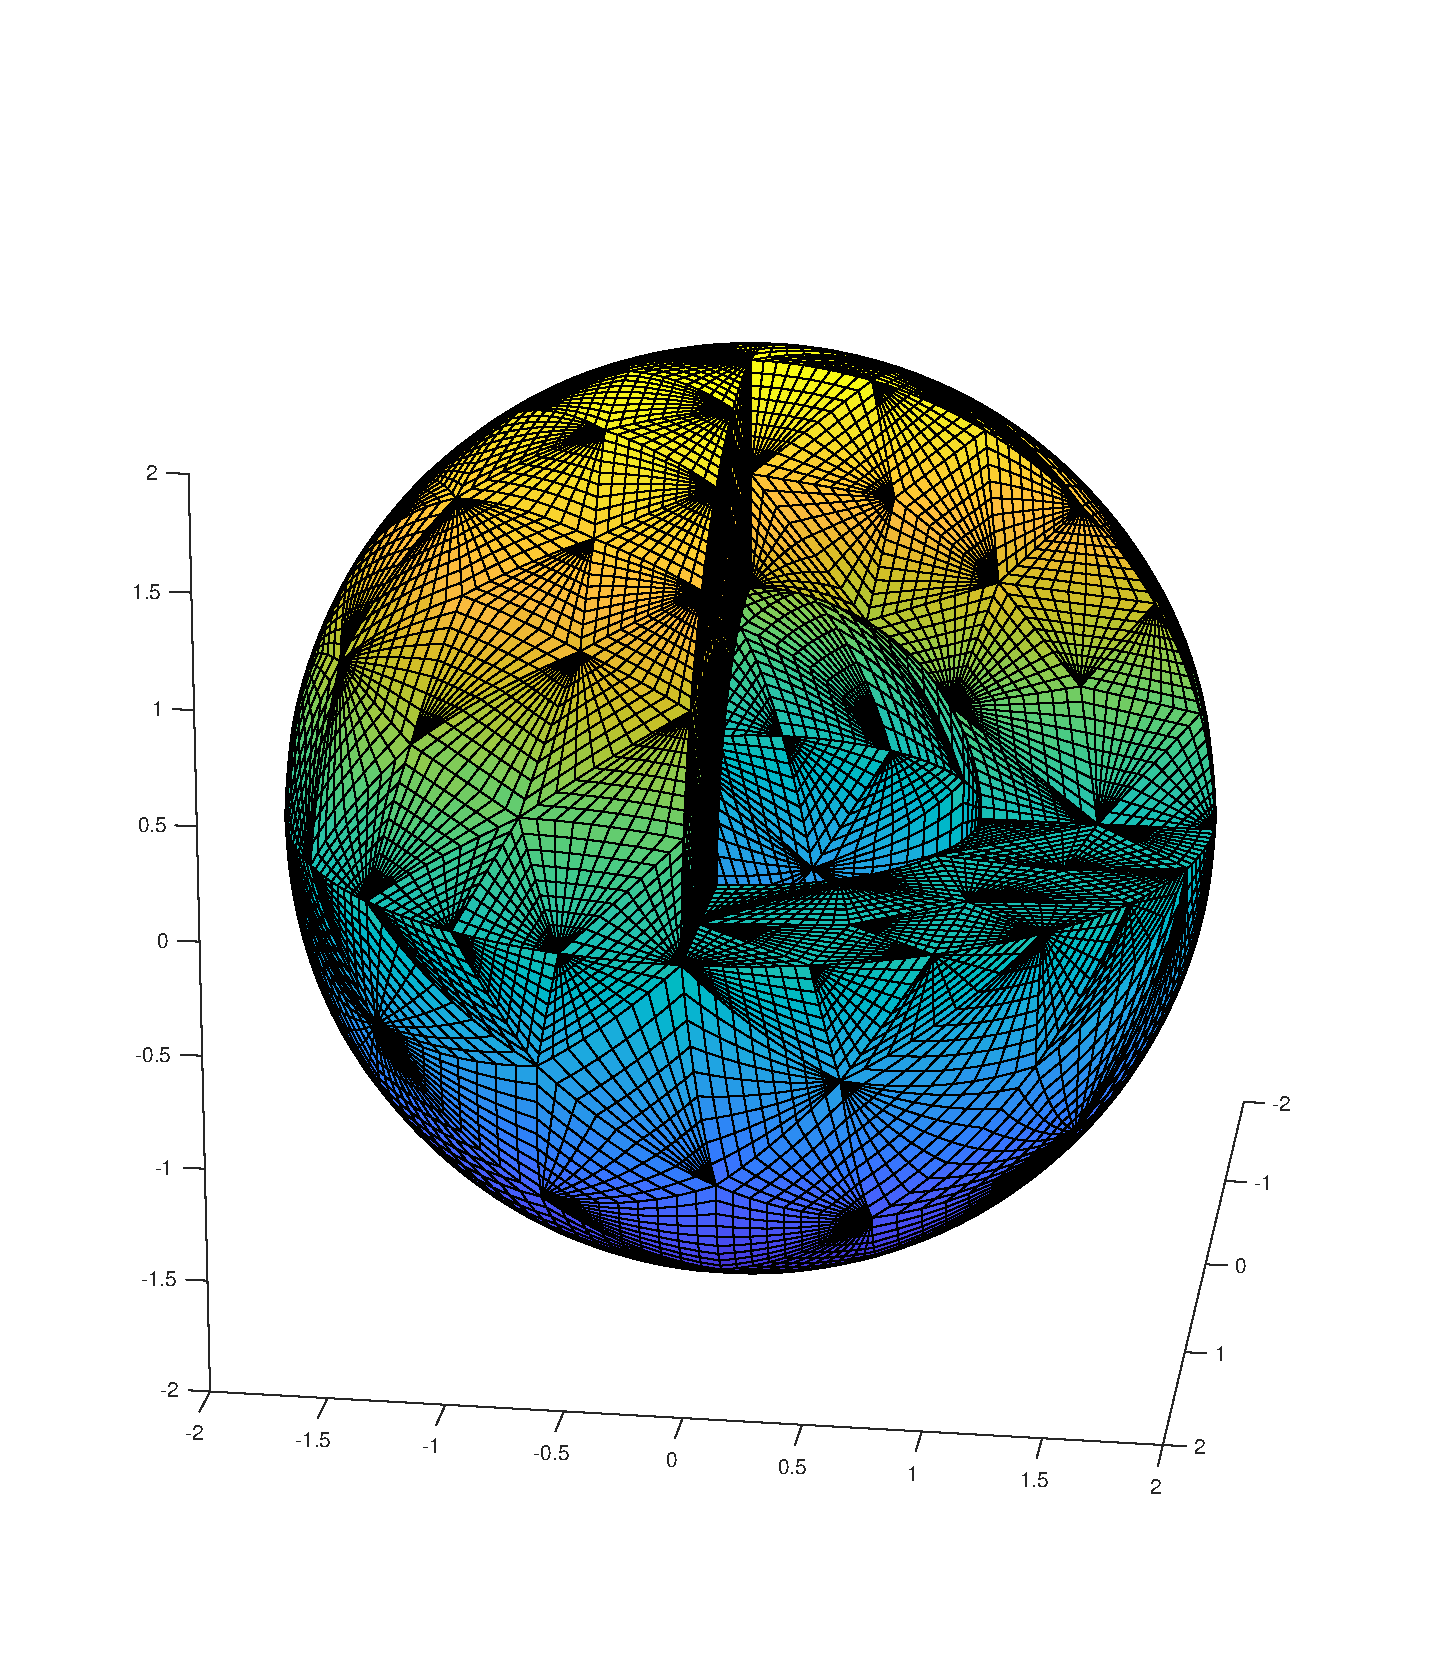
\includegraphics[width=6in]{esfera_esfera_skeleton.pdf}
\end{center}
\caption{esfera\_esfera.msh geometry. Skeleton based on quadratic triangles. The apparent distortion of the triangles is only present in this figure, not in the file (is a plot issue). The set of sources used for the FMM call are 78 Gauss nodes on each quadratic triangle}
\label{esfera_esfera_skeleton}
\end{figure}








\newpage
\subsection{high\_genus.msh (adaptive\_flag=0)}
Example of a geometry with $genus=25$ (figure \ref{high_genus} and \ref{high_genus_skeleton}).

\begin{figure}[H]
\begin{center}
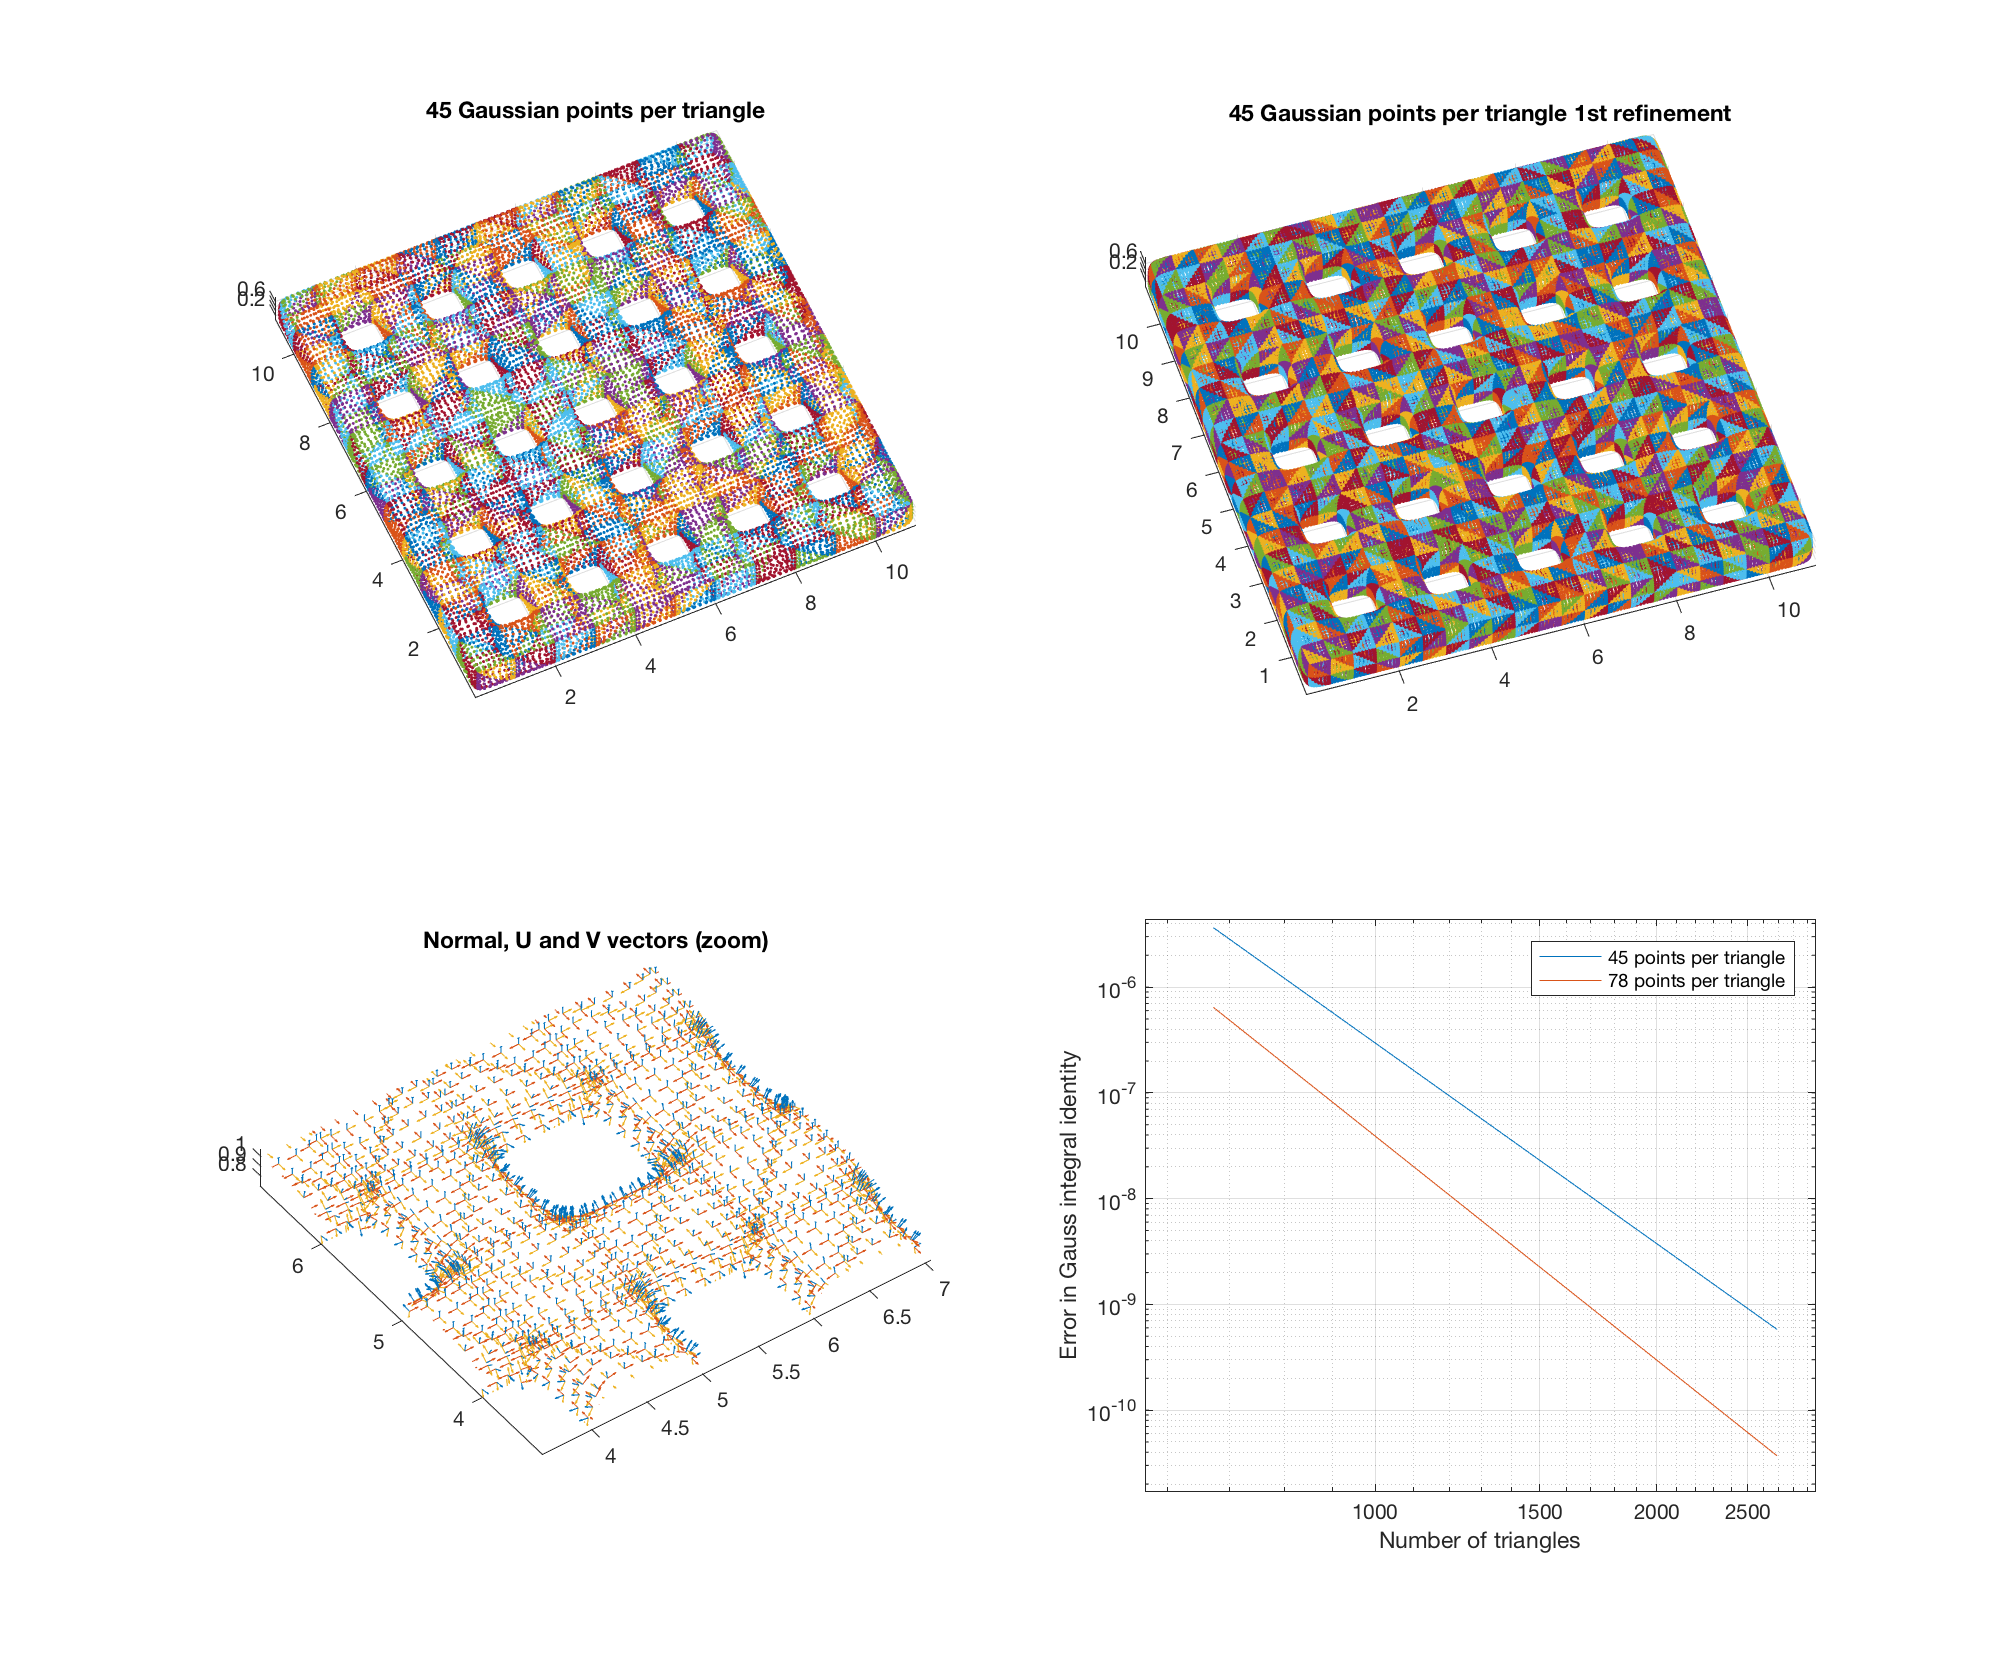
\includegraphics[width=6in]{high_genus.pdf}
\end{center}
\caption{The first row of figures show the refinement process with $n_{refinement}=0, n_{refinement}=1$ respectively.
The figure down-left shows the normal vector and two tangent orthogonal vectors U, V (all unitary) on each discretization point. The figure down-right shows the convergence obtained. }
\label{high_genus}
\end{figure}


\begin{figure}[H]
\begin{center}
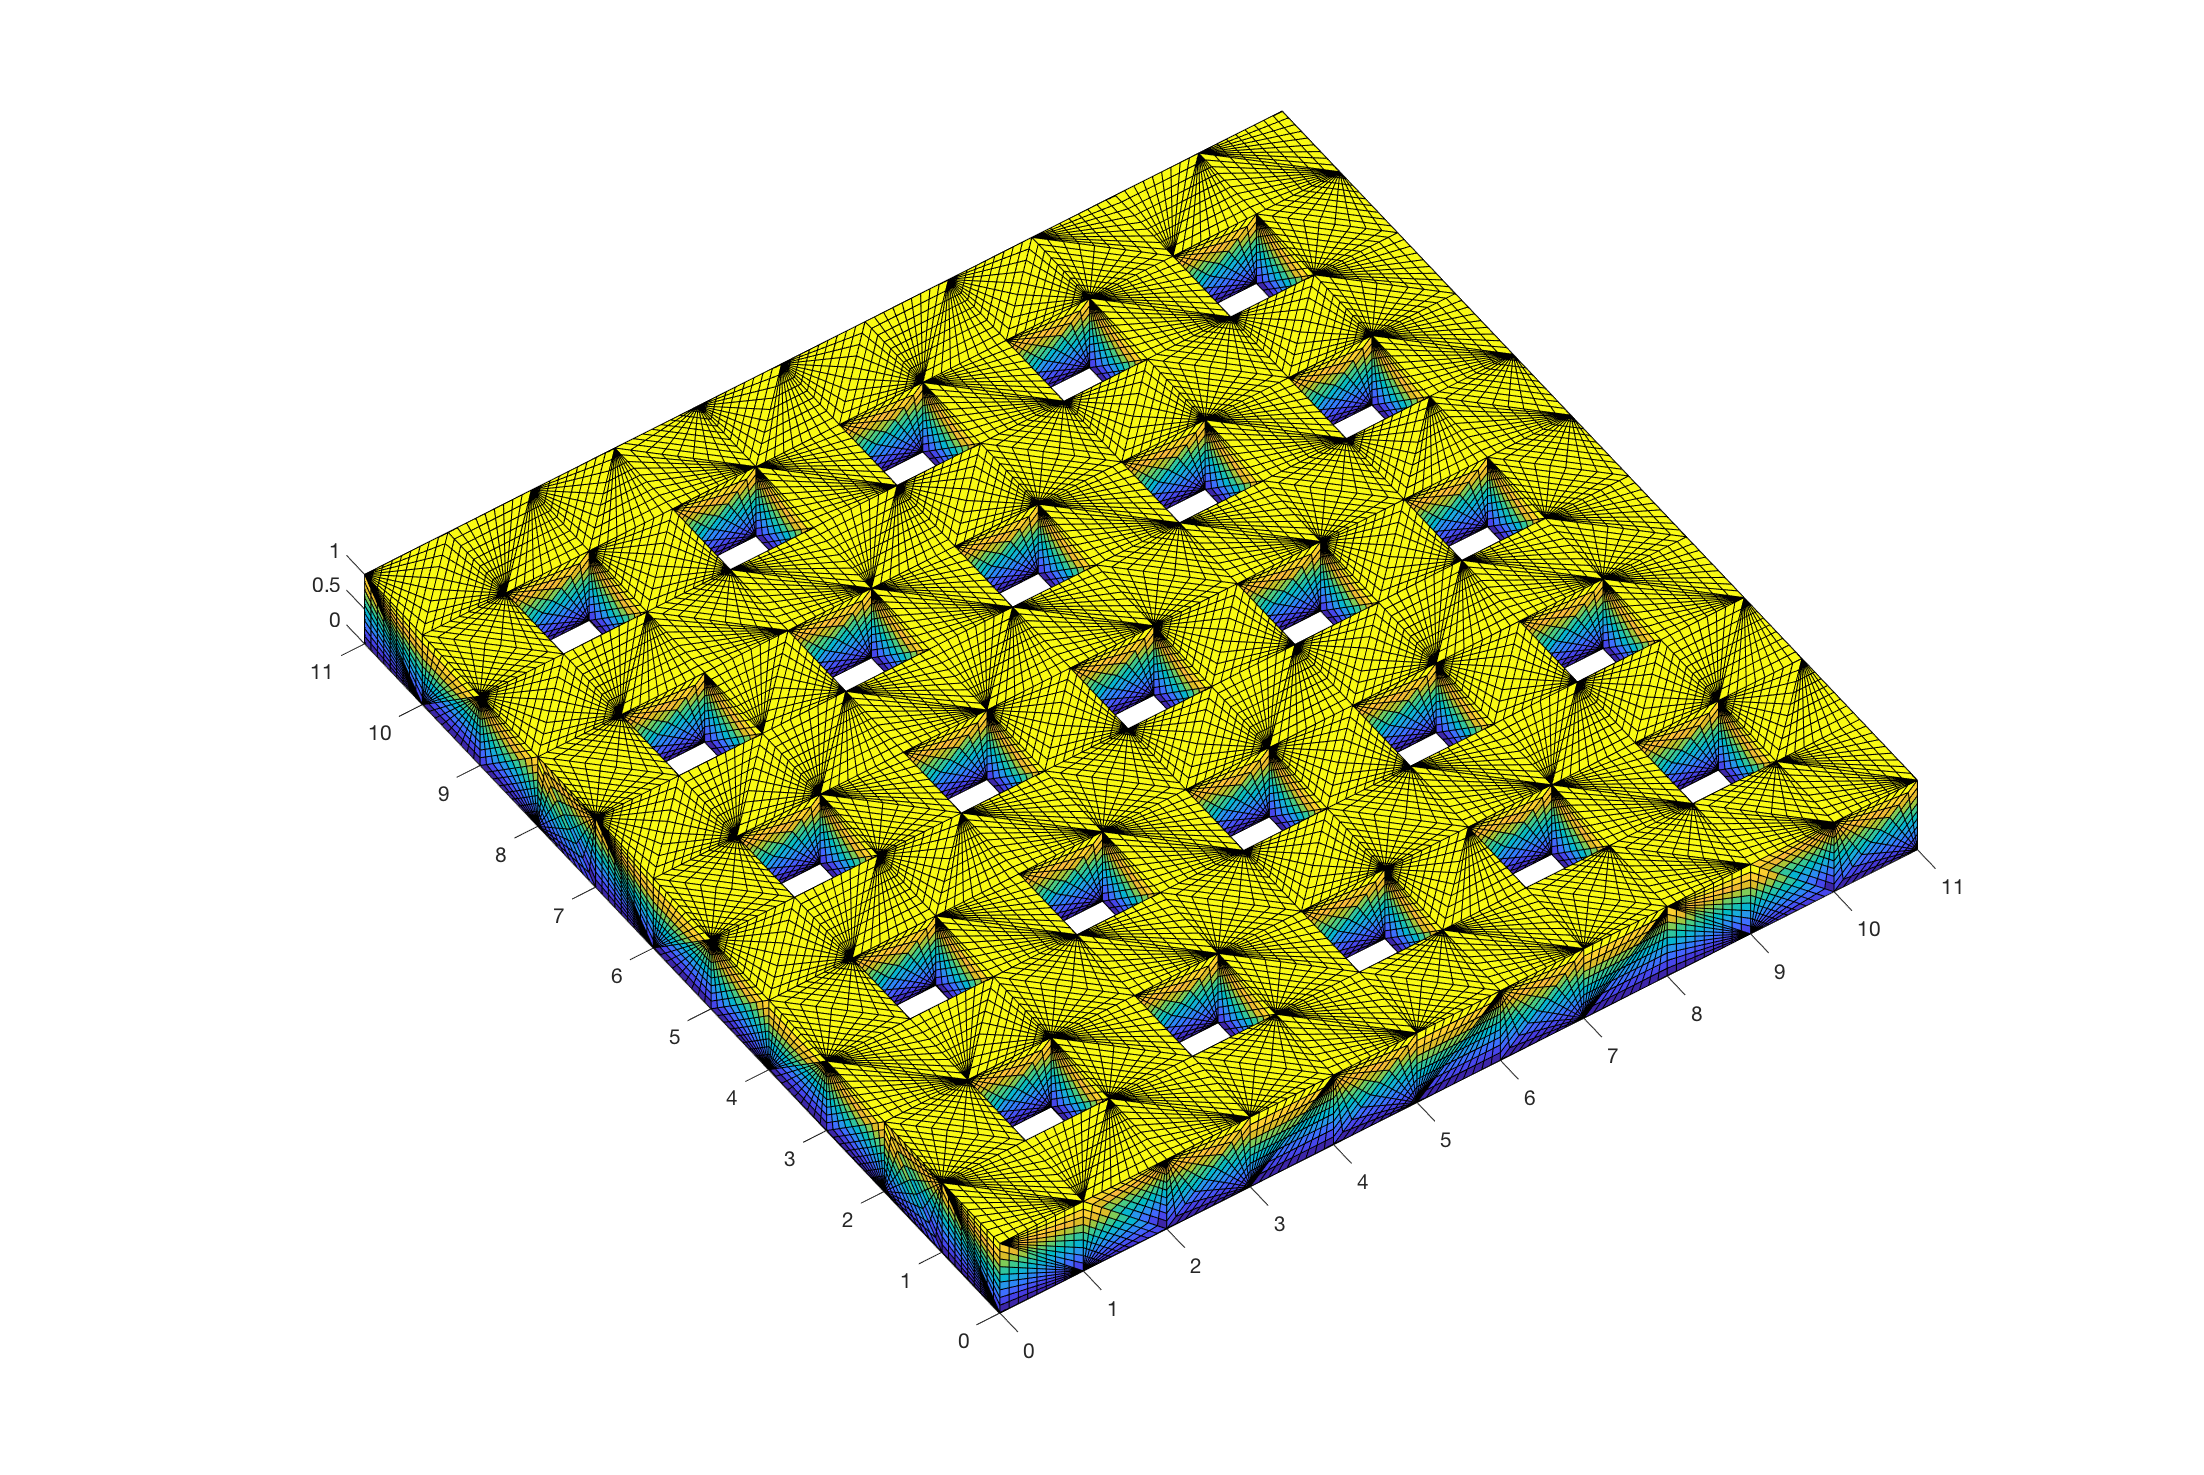
\includegraphics[width=6in]{high_genus_skeleton.pdf}
\end{center}
\caption{high\_genus.msh geometry. Skeleton based on quadratic triangles. The apparent distortion of the triangles is only present in this figure, not in the file (is a plot issue). The set of sources used for the FMM call are 78 Gauss nodes on each quadratic triangle}
\label{high_genus_skeleton}
\end{figure}







\newpage
\subsection{Multiscale\_1.msh (adaptive\_flag=1)}
Simple example with a small detain on top to test adaptivity (figure \ref{Multiscale_1} and \ref{Multiscale_1_skeleton}).

\begin{figure}[H]
\begin{center}
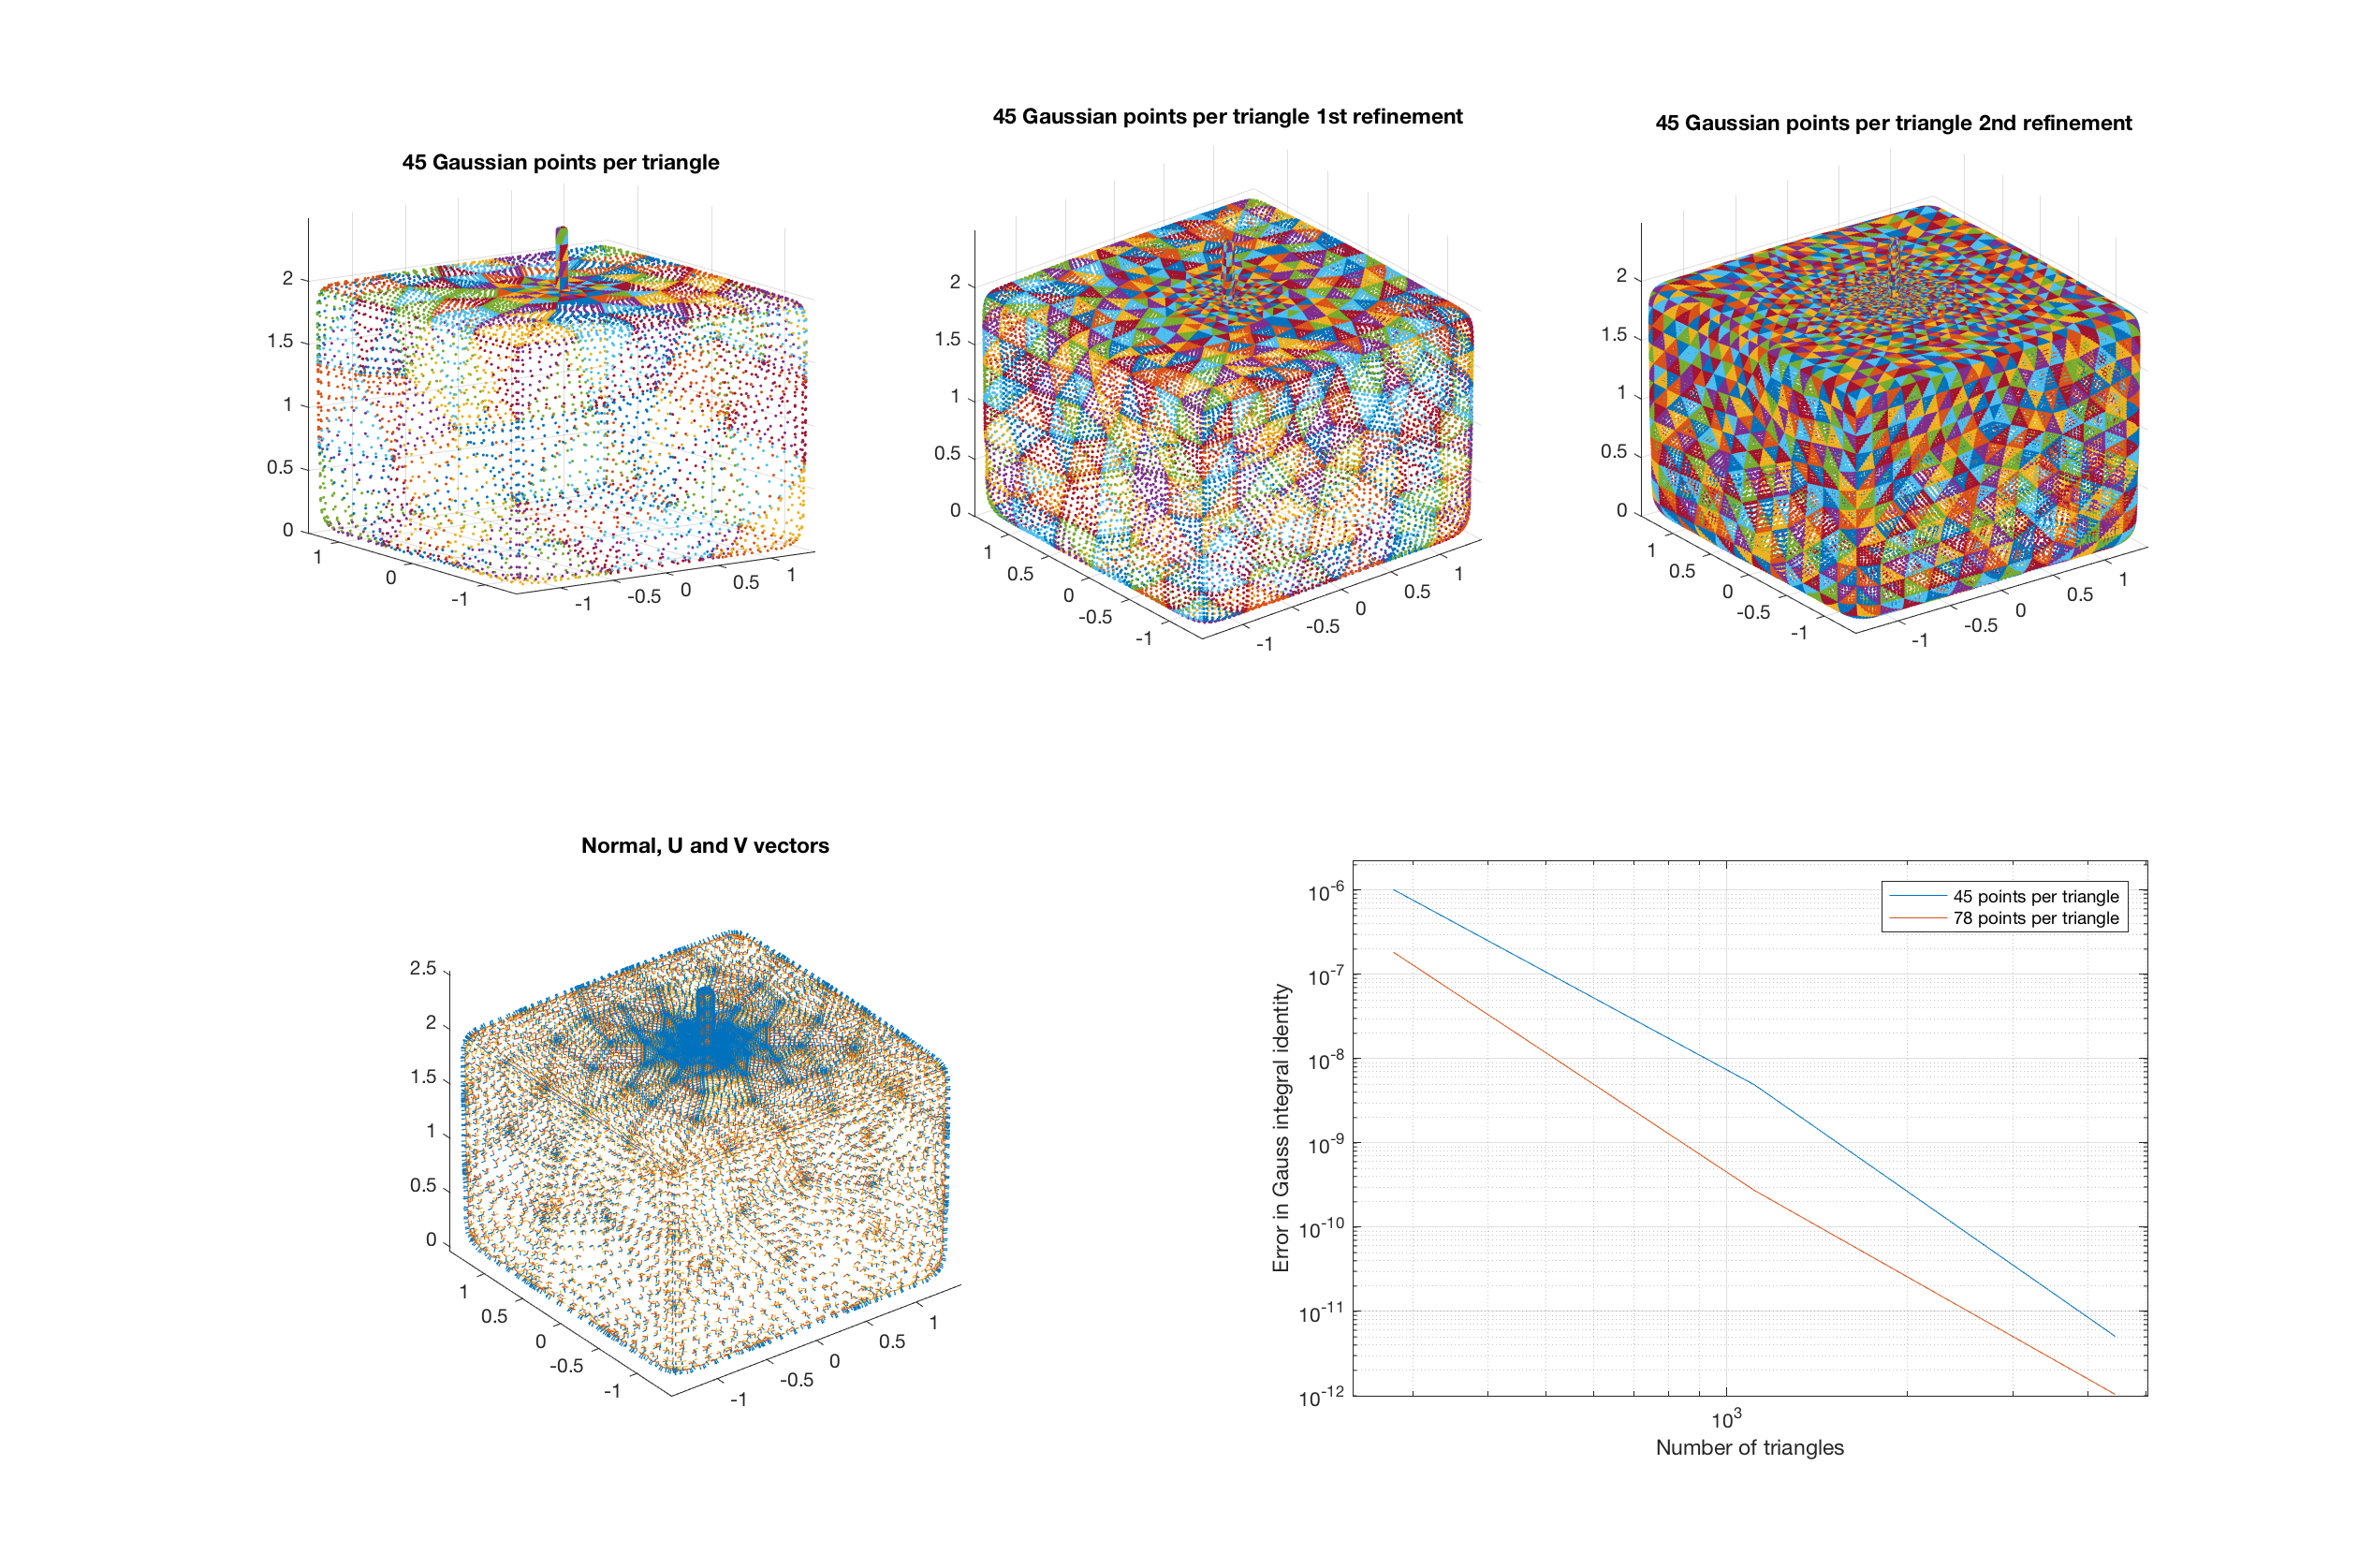
\includegraphics[width=6in]{Multiscale_1.pdf}
\end{center}
\caption{The first row of figures show the refinement process with $n_{refinement}=0, n_{refinement}=1, n_{refinement}=2$ respectively. The figure down left shows the normal vector and two tangent orthogonal vectors U, V (all unitary) on each discretization point. The figure down right shows the convergence obtained.}
\label{Multiscale_1}
\end{figure}


\begin{figure}[H]
\begin{center}
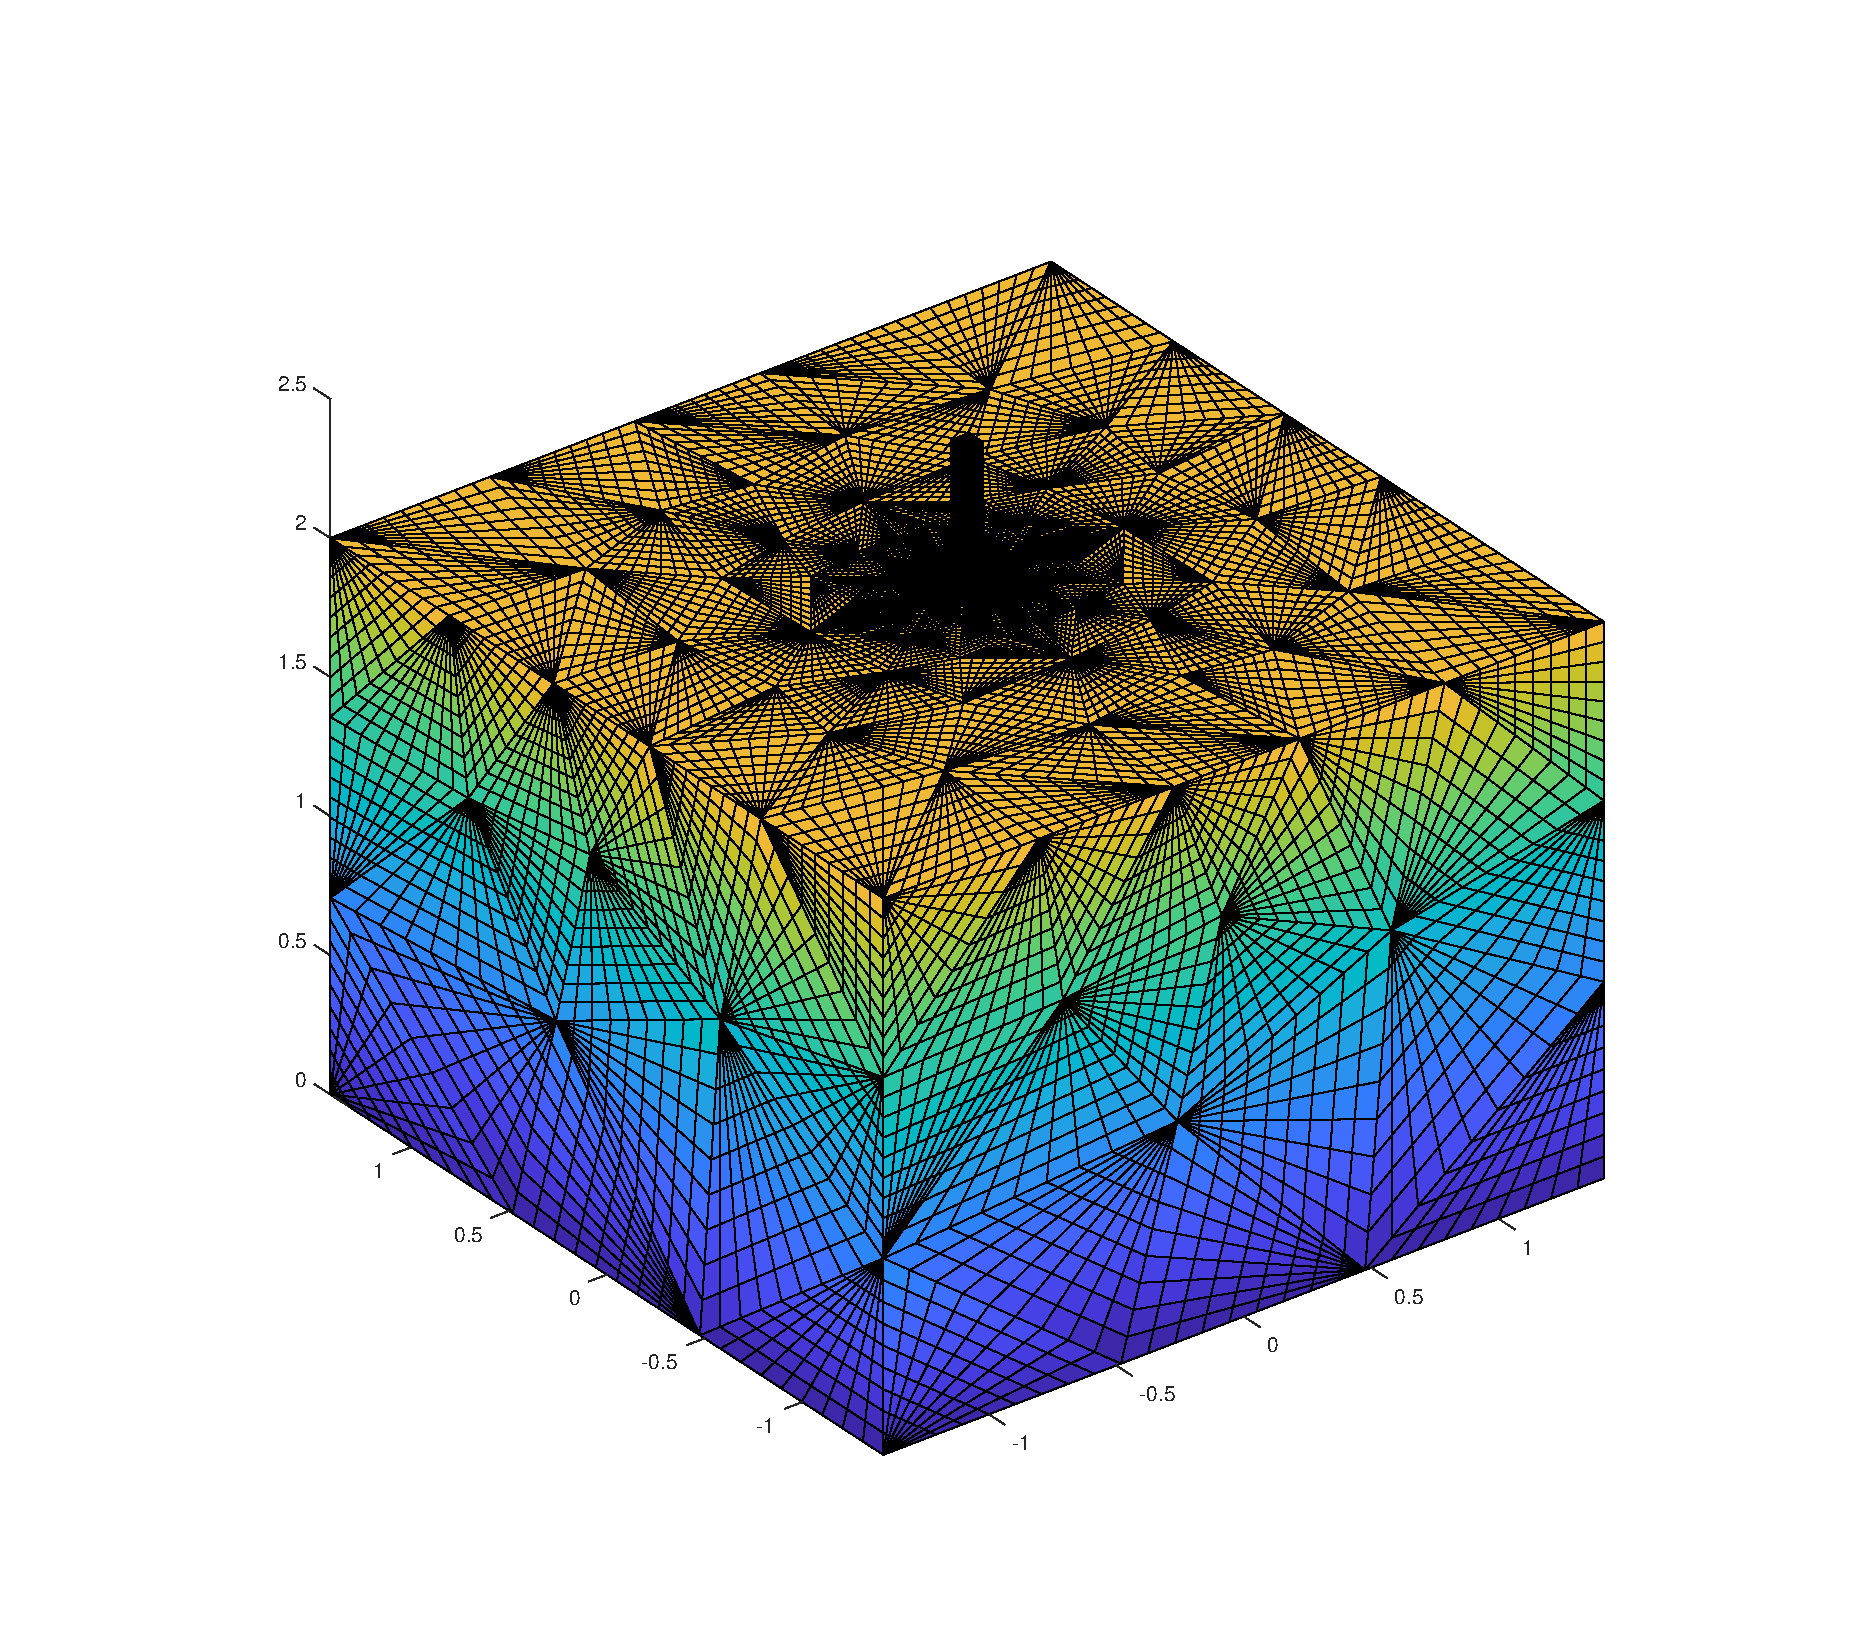
\includegraphics[width=6in]{Multiscale_1_skeleton.pdf}
\end{center}
\caption{Multiscale\_1.msh geometry. Skeleton based on quadratic triangles. The apparent distortion of the triangles is only present in this figure, not in the file (is a plot issue). The set of sources used for the FMM call are 78 Gauss nodes on each quadratic triangle}
\label{Multiscale_1_skeleton}
\end{figure}






\newpage
\subsection{capsule\_multiscale.msh (adaptive\_flag=1)}
Another example with a small detail to test adaptivity (figure \ref{capsule_multiscale} and \ref{capsule_multiscale_skeleton}).

\begin{figure}[H]
\begin{center}
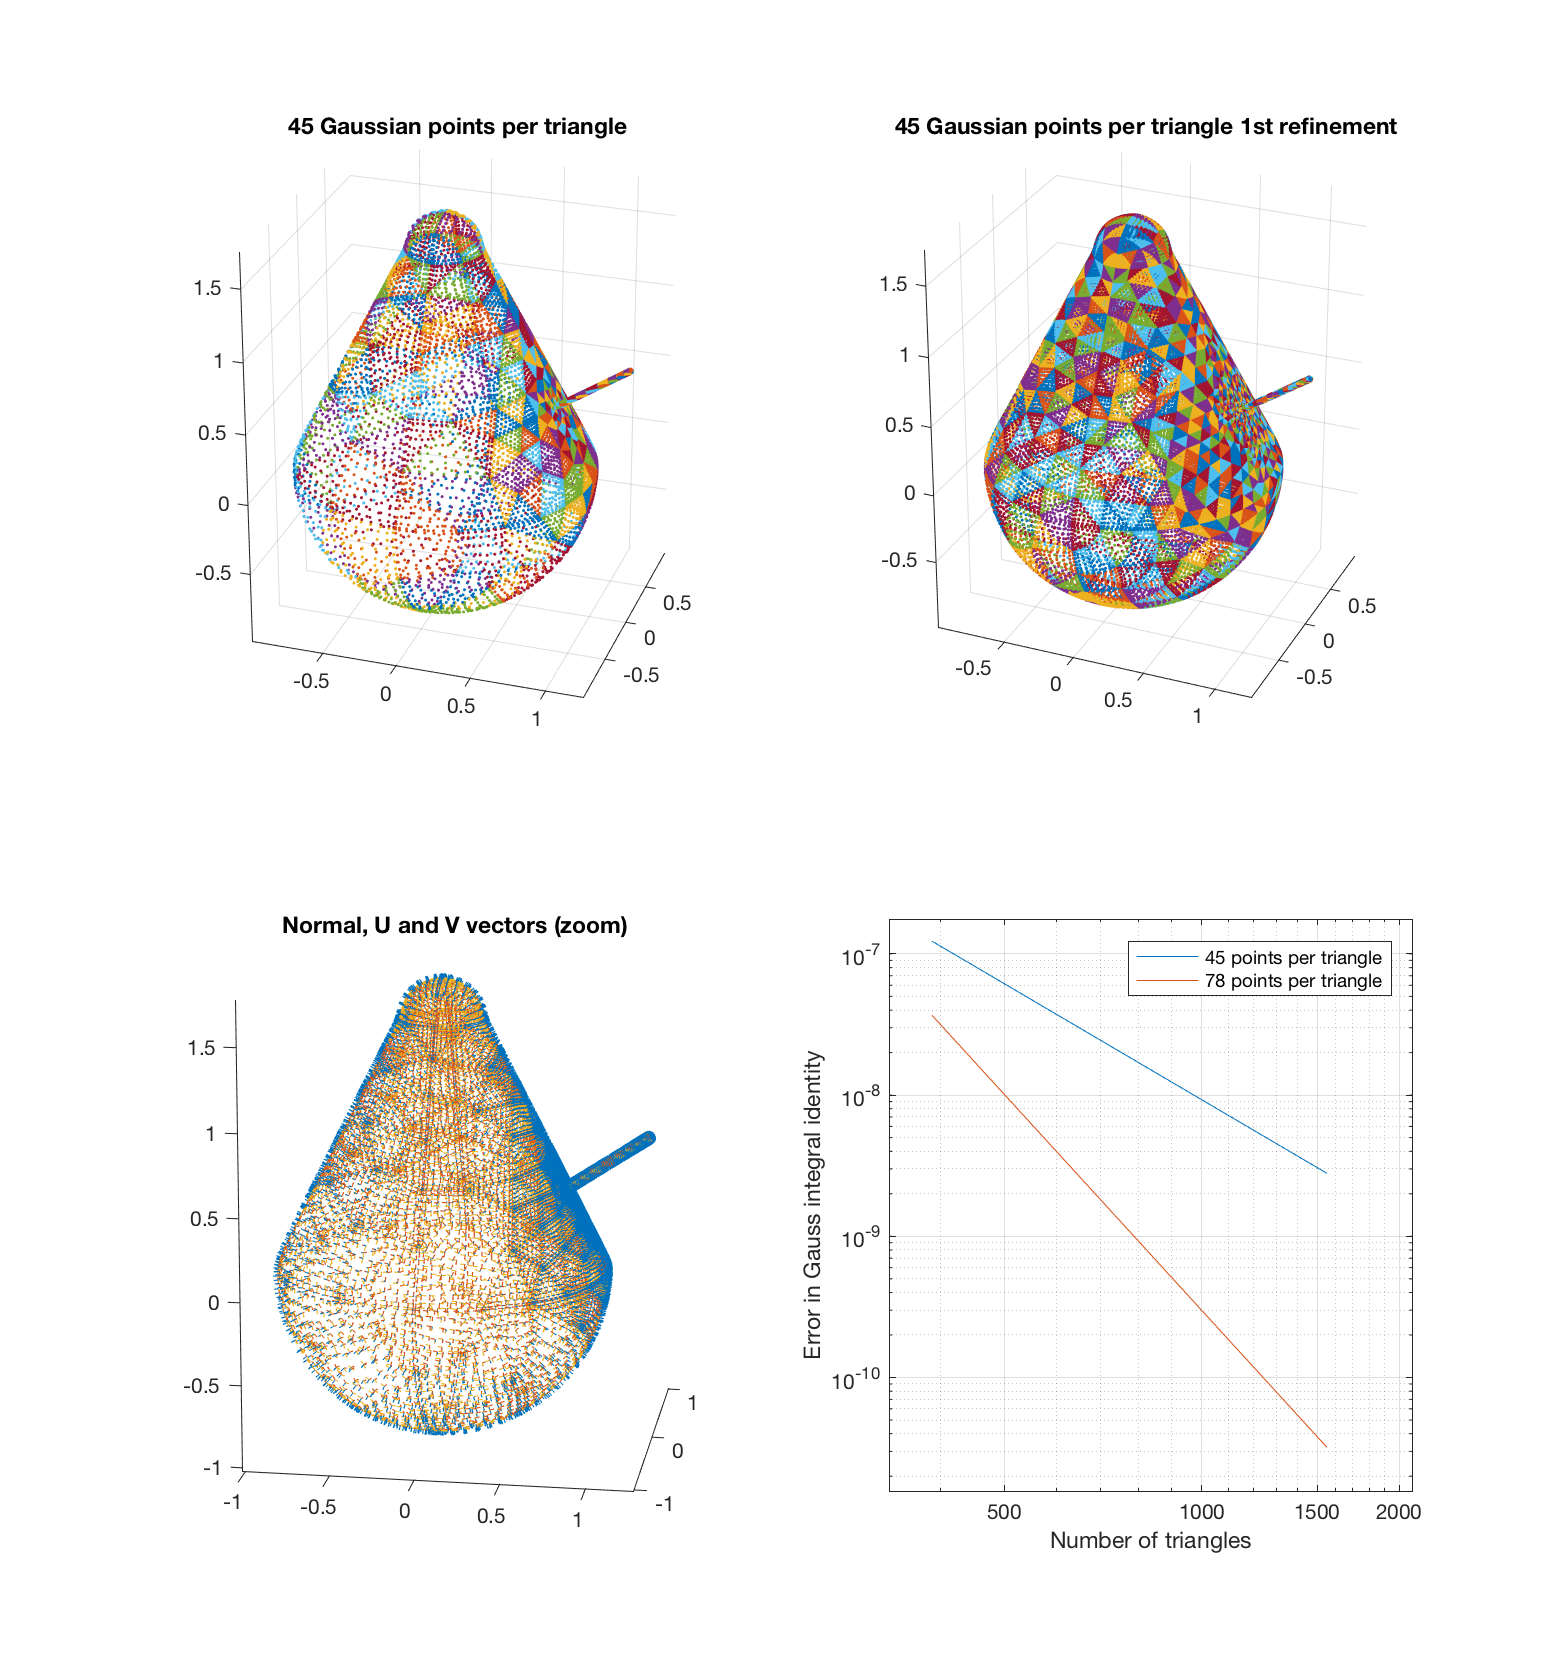
\includegraphics[width=5.5in]{capsule_multiscale.pdf}
\end{center}
\caption{The first row of figures show the refinement process with $n_{refinement}=0, n_{refinement}=1$ respectively.
The figure down left shows the normal vector and two tangent orthogonal vectors U, V (all unitary) on each discretization point. The figure down right shows the convergence obtained. }
\label{capsule_multiscale}
\end{figure}


\begin{figure}[H]
\begin{center}
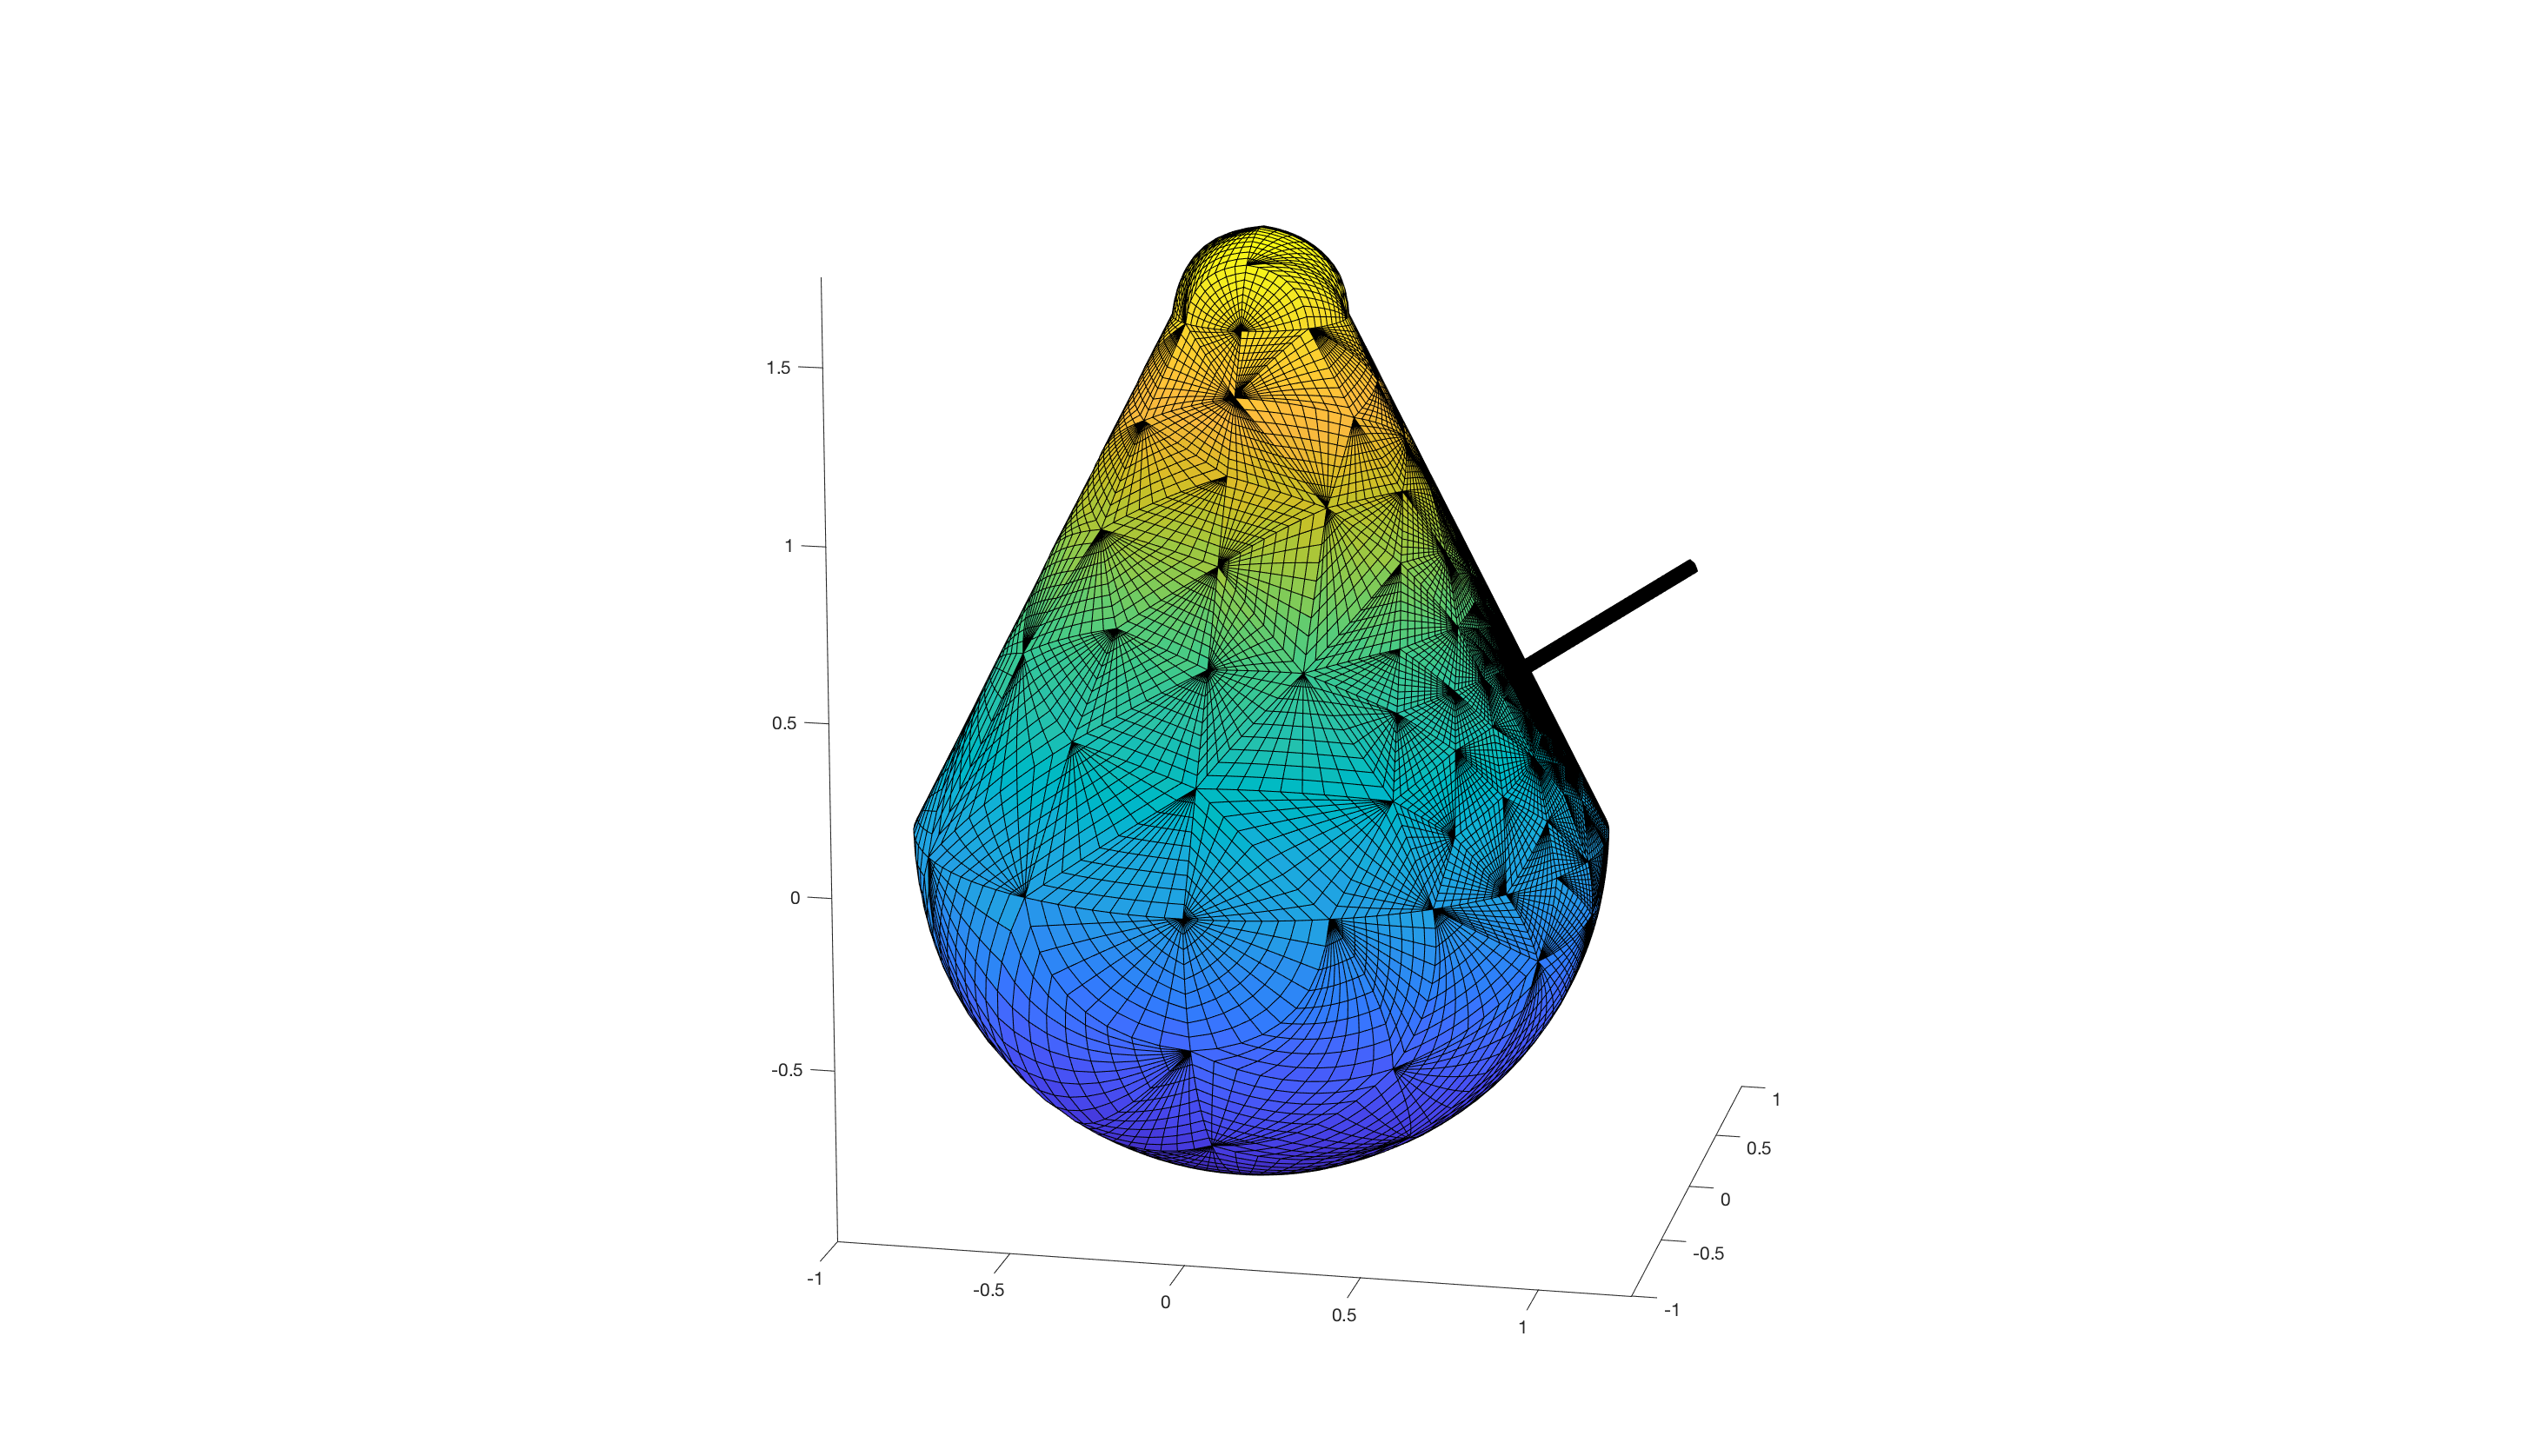
\includegraphics[width=6in]{capsule_multiscale_skeleton.pdf}
\end{center}
\caption{capsule\_multiscale.msh geometry. Skeleton based on quadratic triangles. The apparent distortion of the triangles is only present in this figure, not in the file (is a plot issue). The set of sources used for the FMM call are 78 Gauss nodes on each quadratic triangle}
\label{capsule_multiscale_skeleton}
\end{figure}






\newpage
\subsection{cubo\_esfera\_multires.msh (adaptive\_flag=1)}
Example of a geometry with a spherical cavity and a small detail inside the cavity (figure \ref{cubo_esfera_multires} and \ref{cubo_esfera_multires_skeleton}).

\begin{figure}[H]
\begin{center}
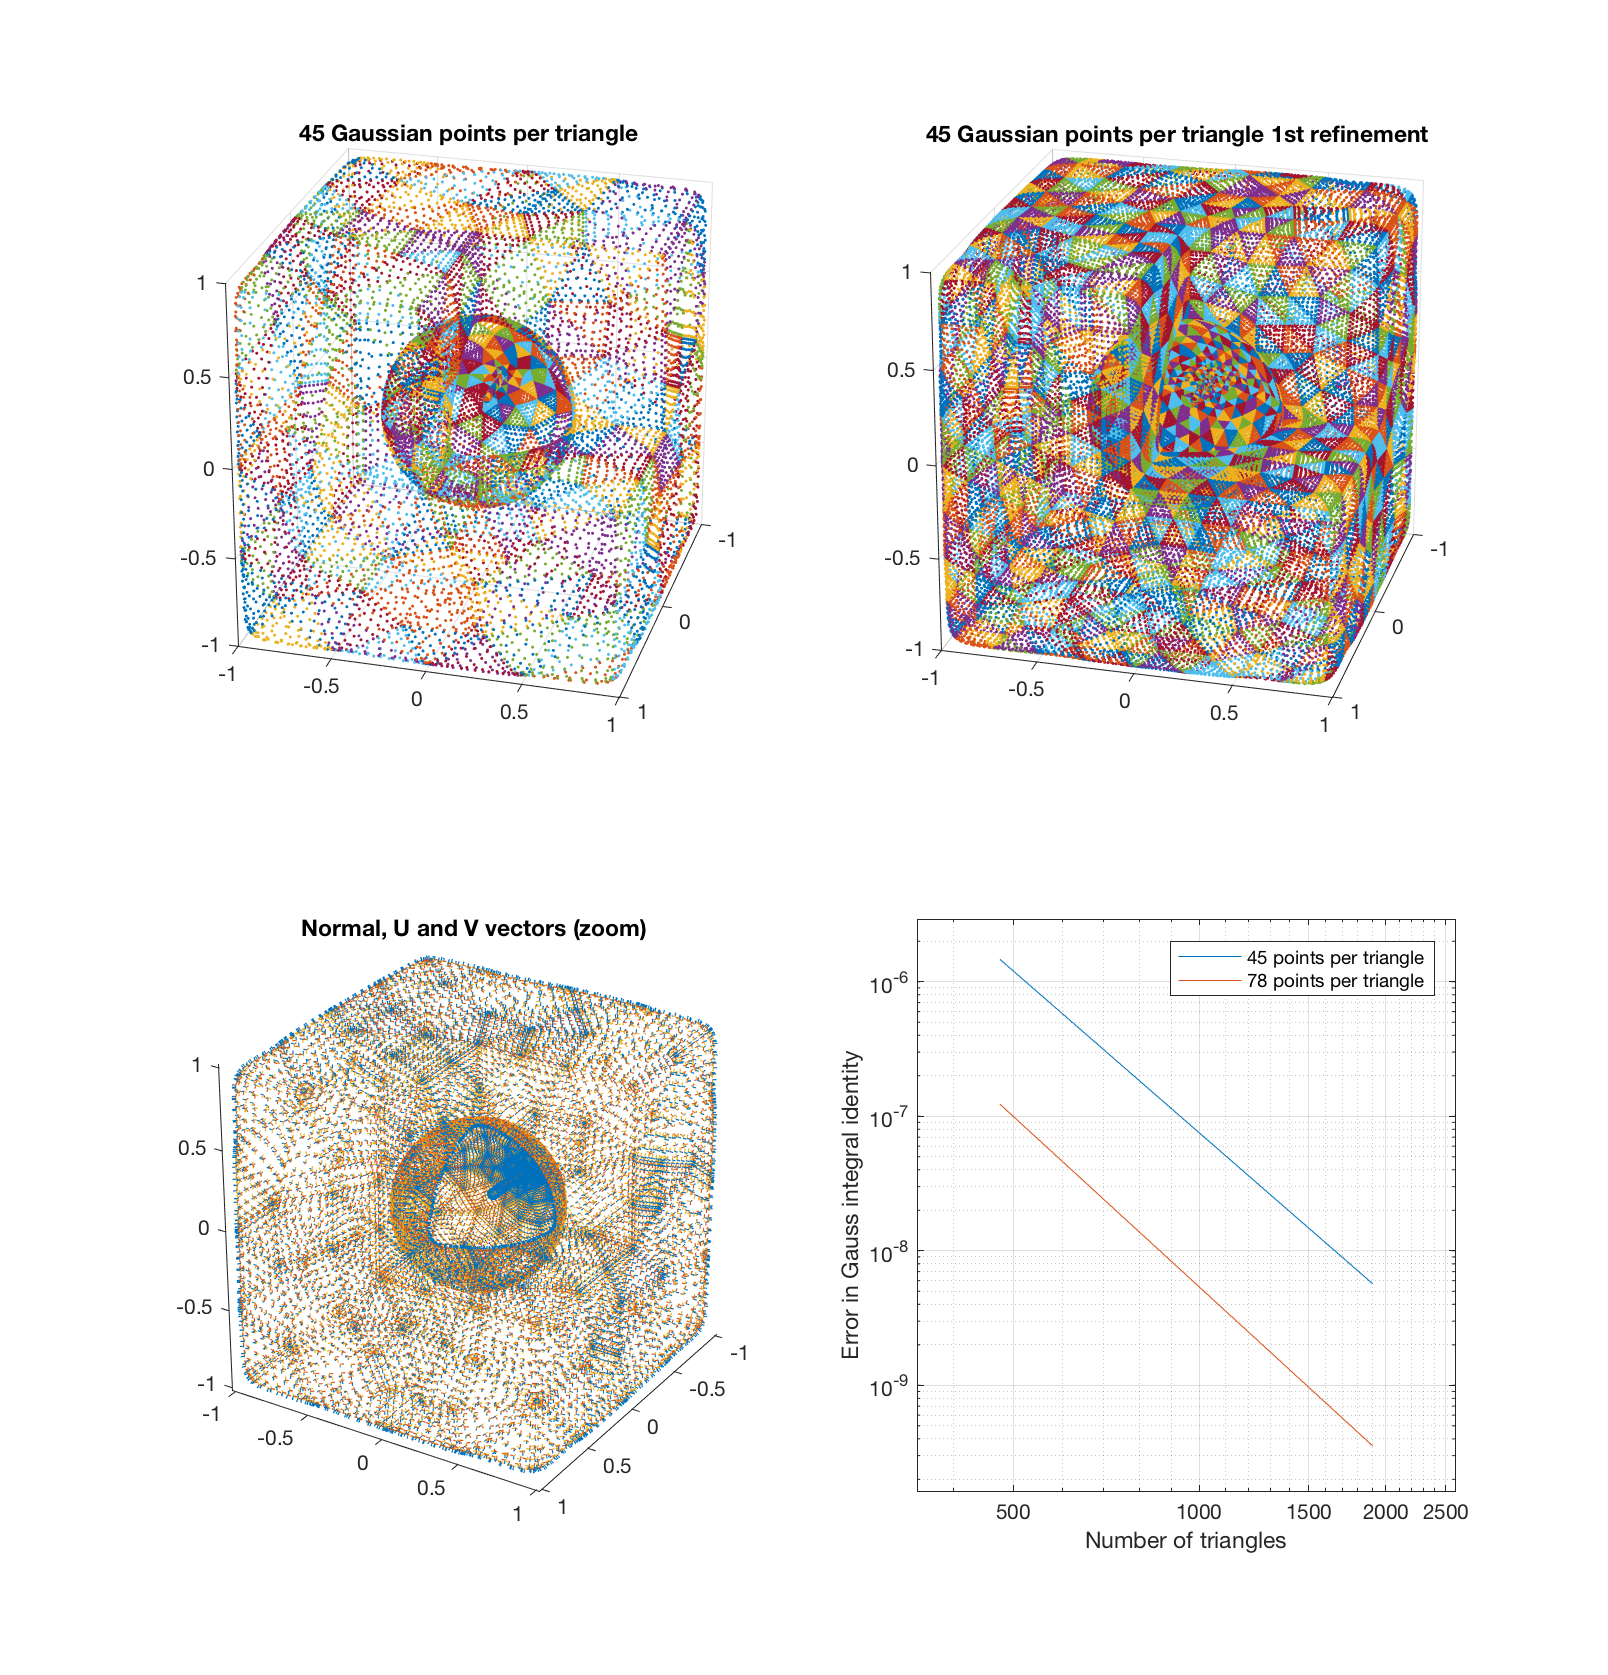
\includegraphics[width=5.5in]{cubo_esfera_multires.pdf}
\end{center}
\caption{The first row of figures show the refinement process with $n_{refinement}=0, n_{refinement}=1$ respectively.
The figure down left shows the normal vector and two tangent orthogonal vectors U, V (all unitary) on each discretization point. The figure down right shows the convergence obtained. }
\label{cubo_esfera_multires}
\end{figure}


\begin{figure}[H]
\begin{center}
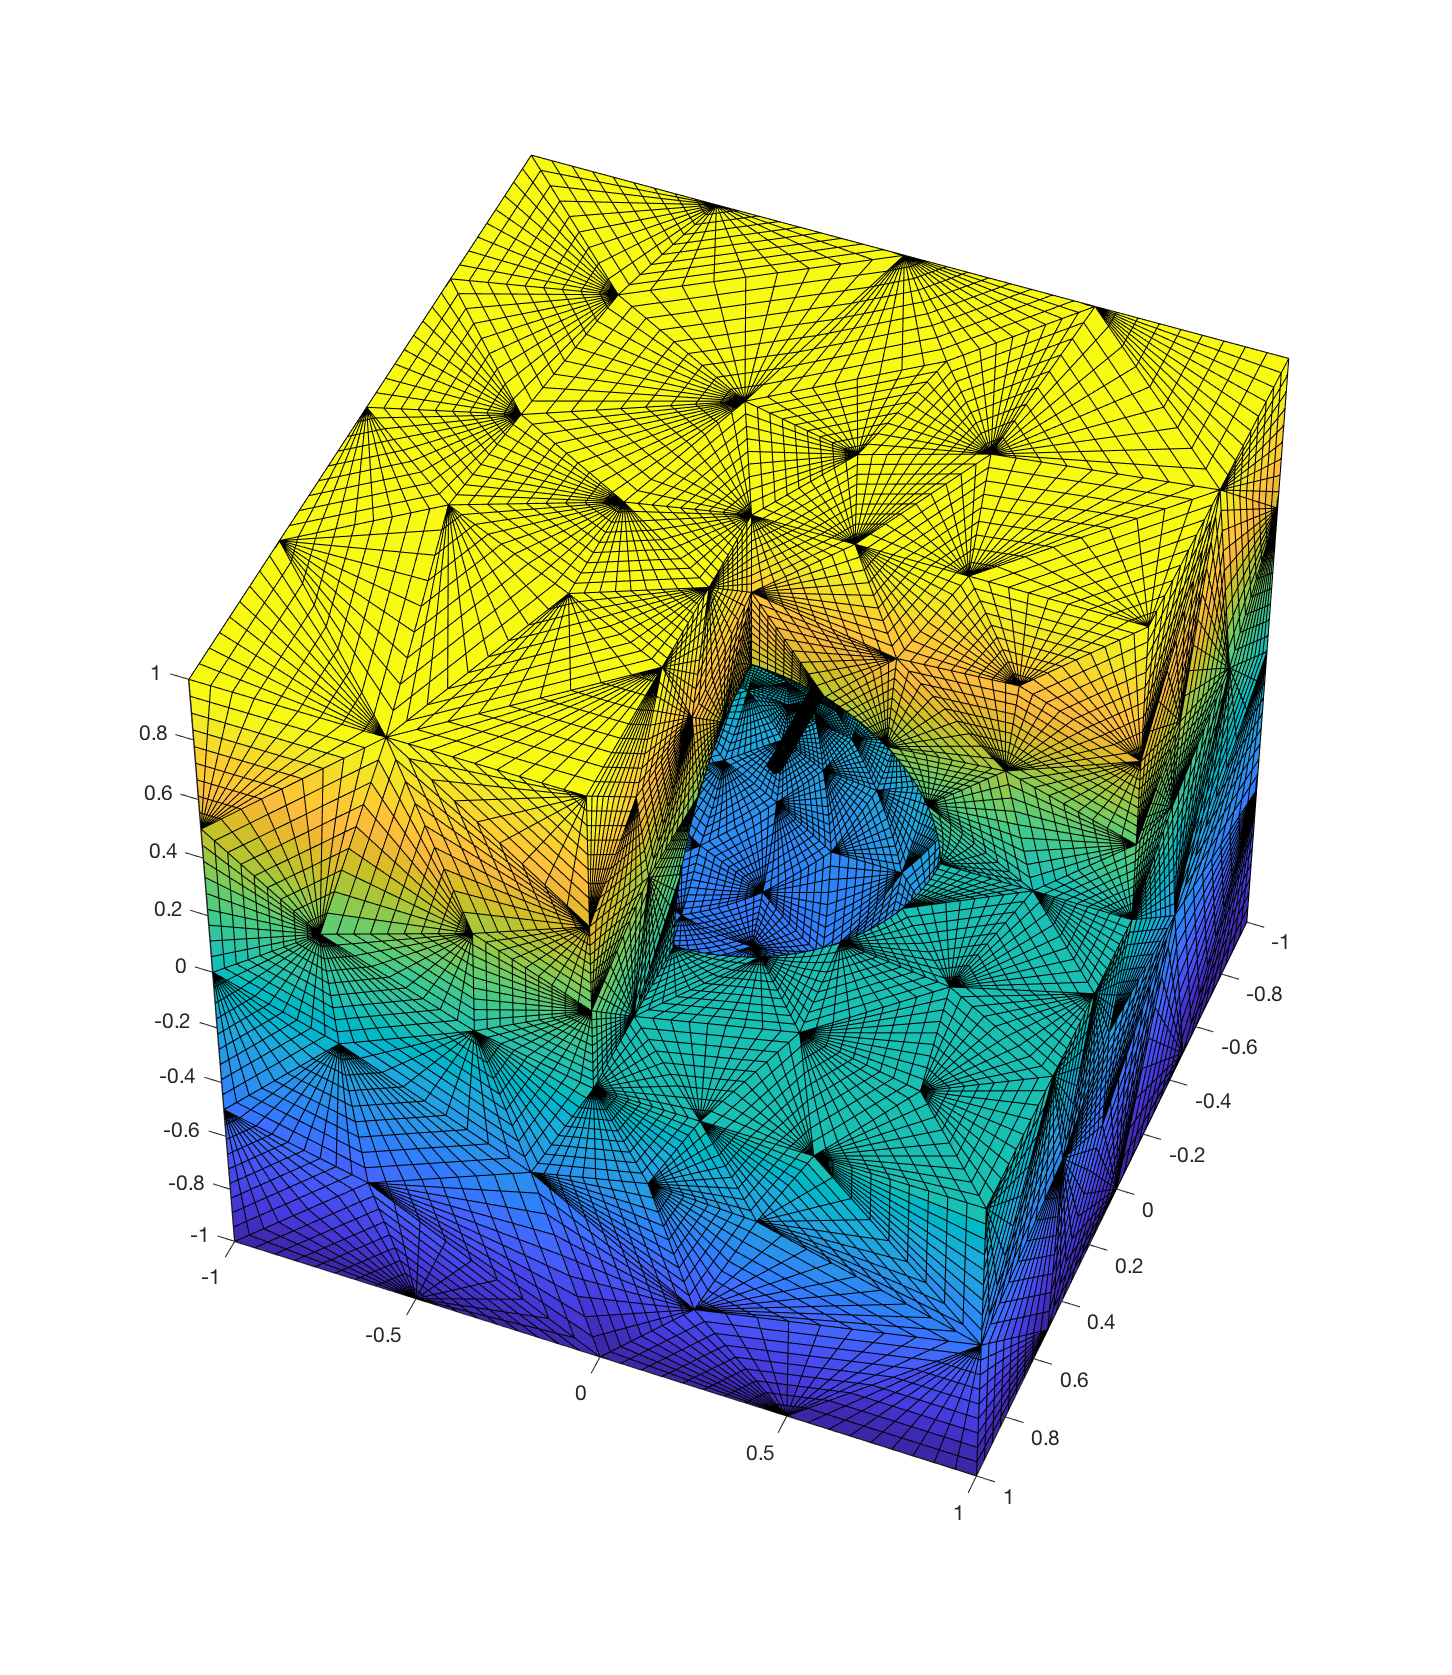
\includegraphics[width=6in]{cubo_esfera_multires_skeleton_1.pdf}
\end{center}
\caption{cubo\_esfera\_multires.msh geometry. Skeleton based on quadratic triangles. We see the small detail inside the inner spherical cavity. The apparent distortion of the triangles is only present in this figure, not in the file (is a plot issue). The set of sources used for the FMM call are 78 Gauss nodes on each quadratic triangle}
\label{cubo_esfera_multires_skeleton}
\end{figure}


\begin{figure}[H]
\begin{center}
\includegraphics[width=6in]{cubo_esfera_multires_skeleton_2.png}
\end{center}
\caption{cubo\_esfera\_multires.msh geometry. Skeleton based on quadratic triangles. We see the small detail inside the inner spherical cavity. The apparent distortion of the triangles is only present in this figure, not in the file (is a plot issue). The set of sources used for the FMM call are 78 Gauss nodes on each quadratic triangle}
\label{cubo_esfera_multires_skeleton}
\end{figure}













\newpage
\subsection{pico\_2.msh (adaptive\_flag=1)}
Geometry with a sharp peak (figure \ref{pico_2} and \ref{pico_2_skeleton}). This is to show that sharp peaks are possible avoiding the caustic effect if we round the skeleton and refine the skeleton when approaching to the peak.



\begin{figure}[H]
\begin{center}
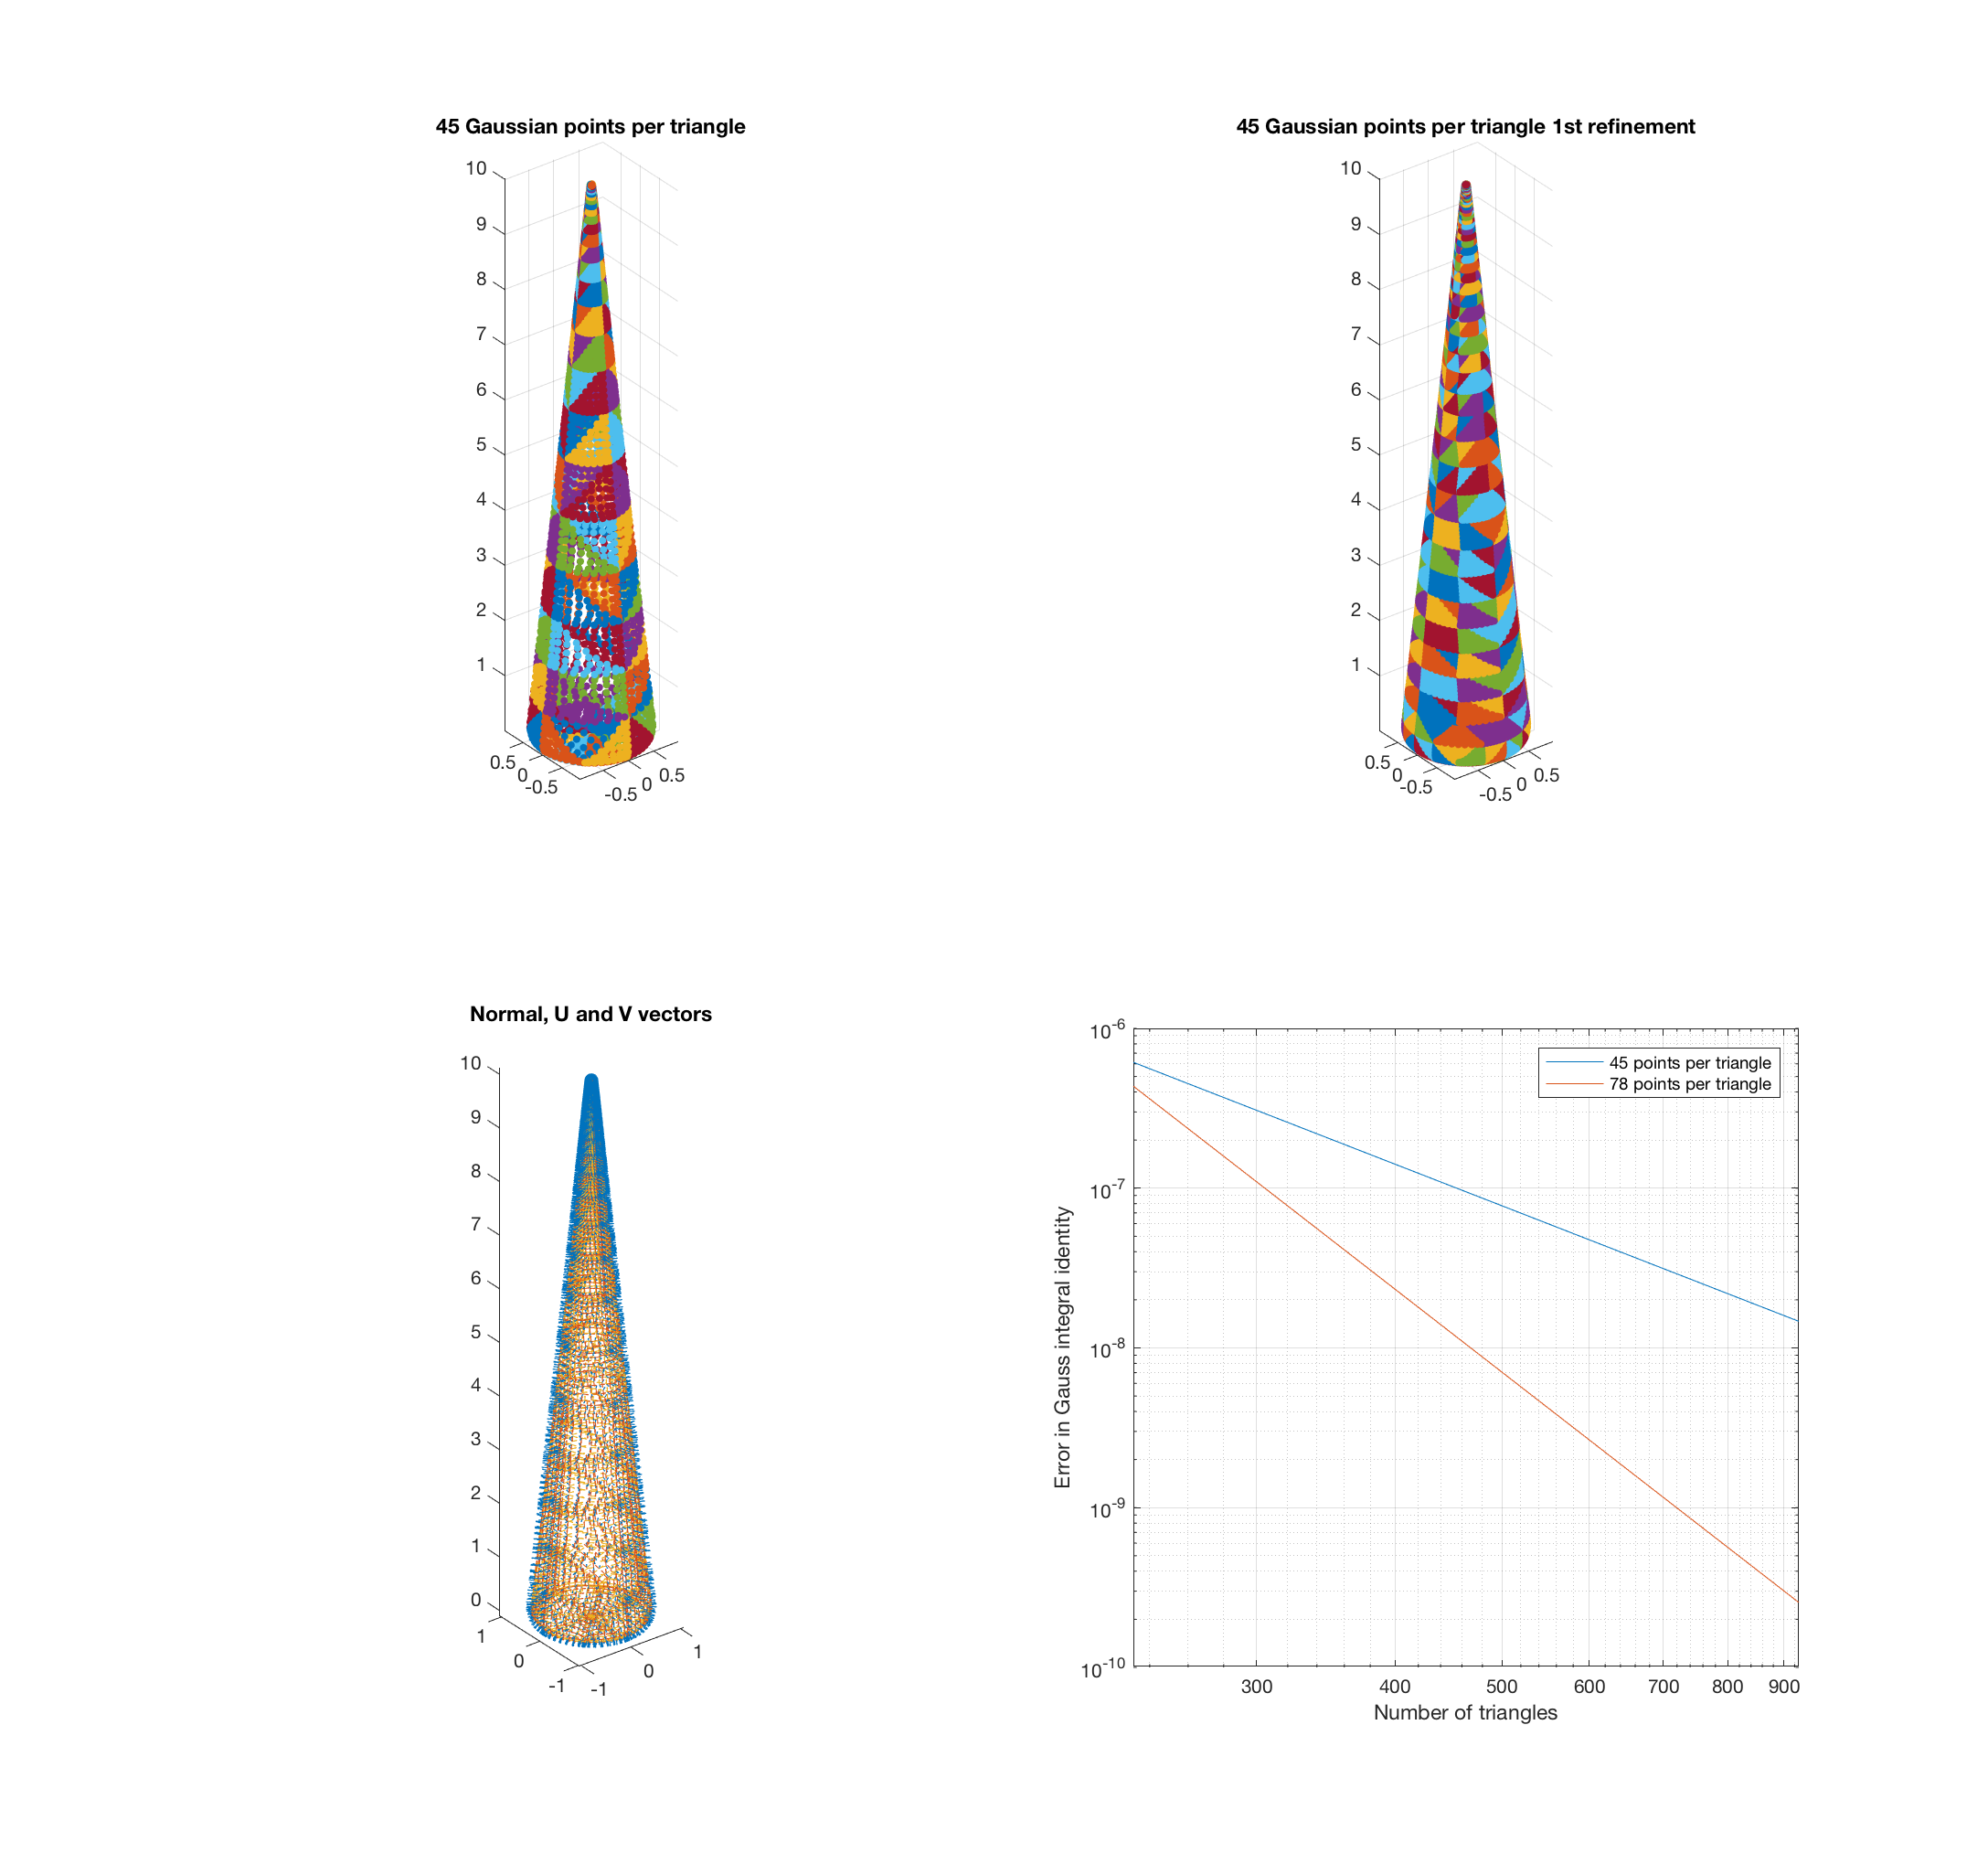
\includegraphics[width=5.6in]{pico_2.pdf}
\end{center}
\caption{The first row of figures show the refinement process with $n_{refinement}=0, n_{refinement}=1$ respectively.
The figure down left shows the normal vector and two tangent orthogonal vectors U, V (all unitary) on each discretization point. The figure down right shows the convergence obtained.}
\label{pico_2}
\end{figure}


\begin{figure}[H]
\begin{center}
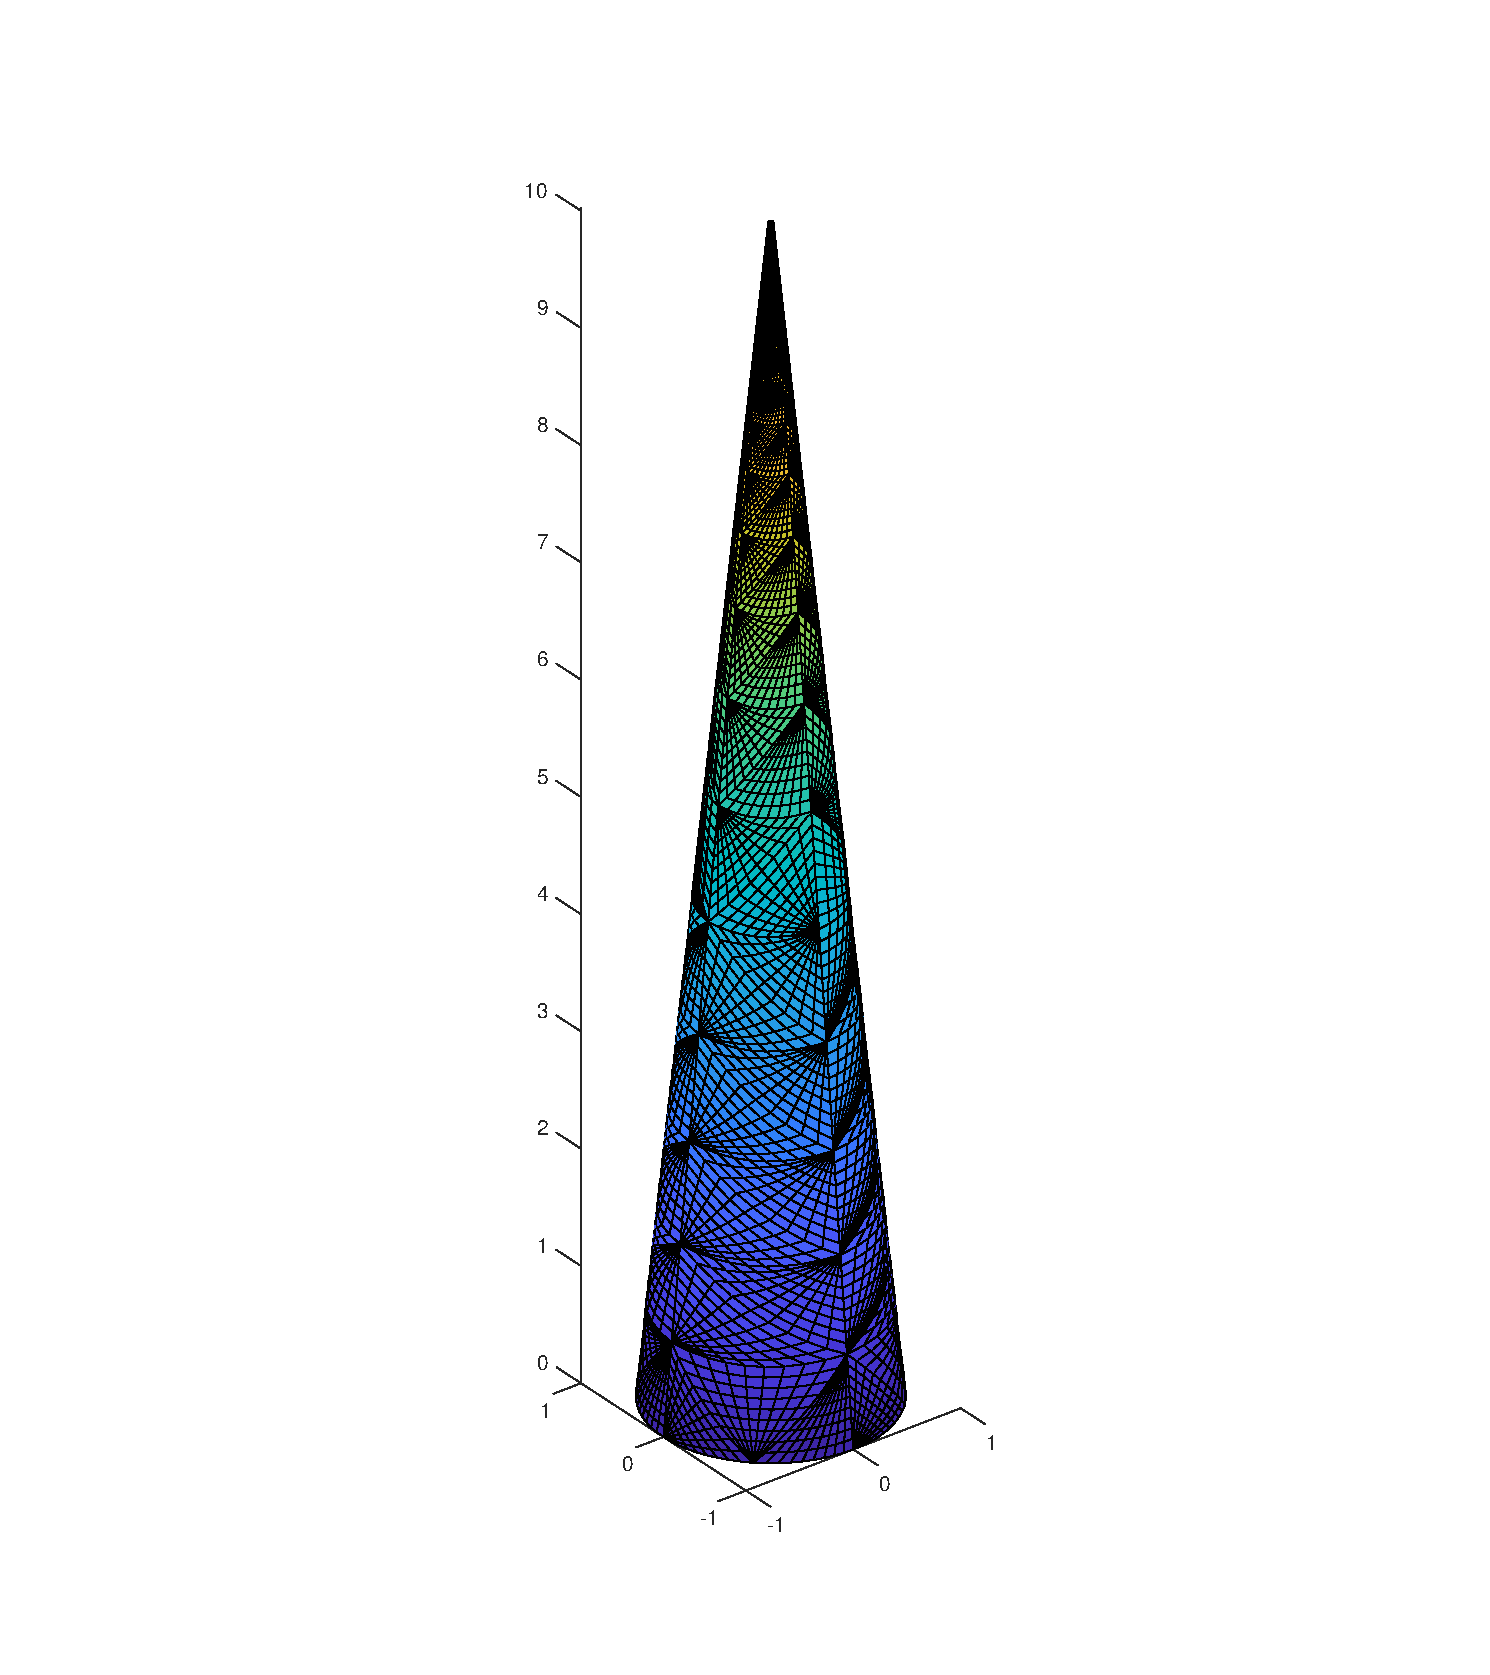
\includegraphics[width=6in]{pico_2_skeleton.pdf}
\end{center}
\caption{pico\_2.msh geometry. Skeleton based on quadratic triangles. The apparent distortion of the triangles is only present in this figure, not in the file (is a plot issue). The set of sources used for the FMM call are 78 Gauss nodes on each quadratic triangle}
\label{pico_2_skeleton}
\end{figure}



\subsection{sci\_fi\_2.msh (adaptive\_flag=0)}
Another example of a complex geometry. Genus 12 and complex tubular conections. No refinement study yet, accuracy obtained for $n_{refinement}=0$ and n\_order\_sf=45 is $Err=5.8\cdot 10^{-8}$
\begin{figure}[H]
\begin{center}
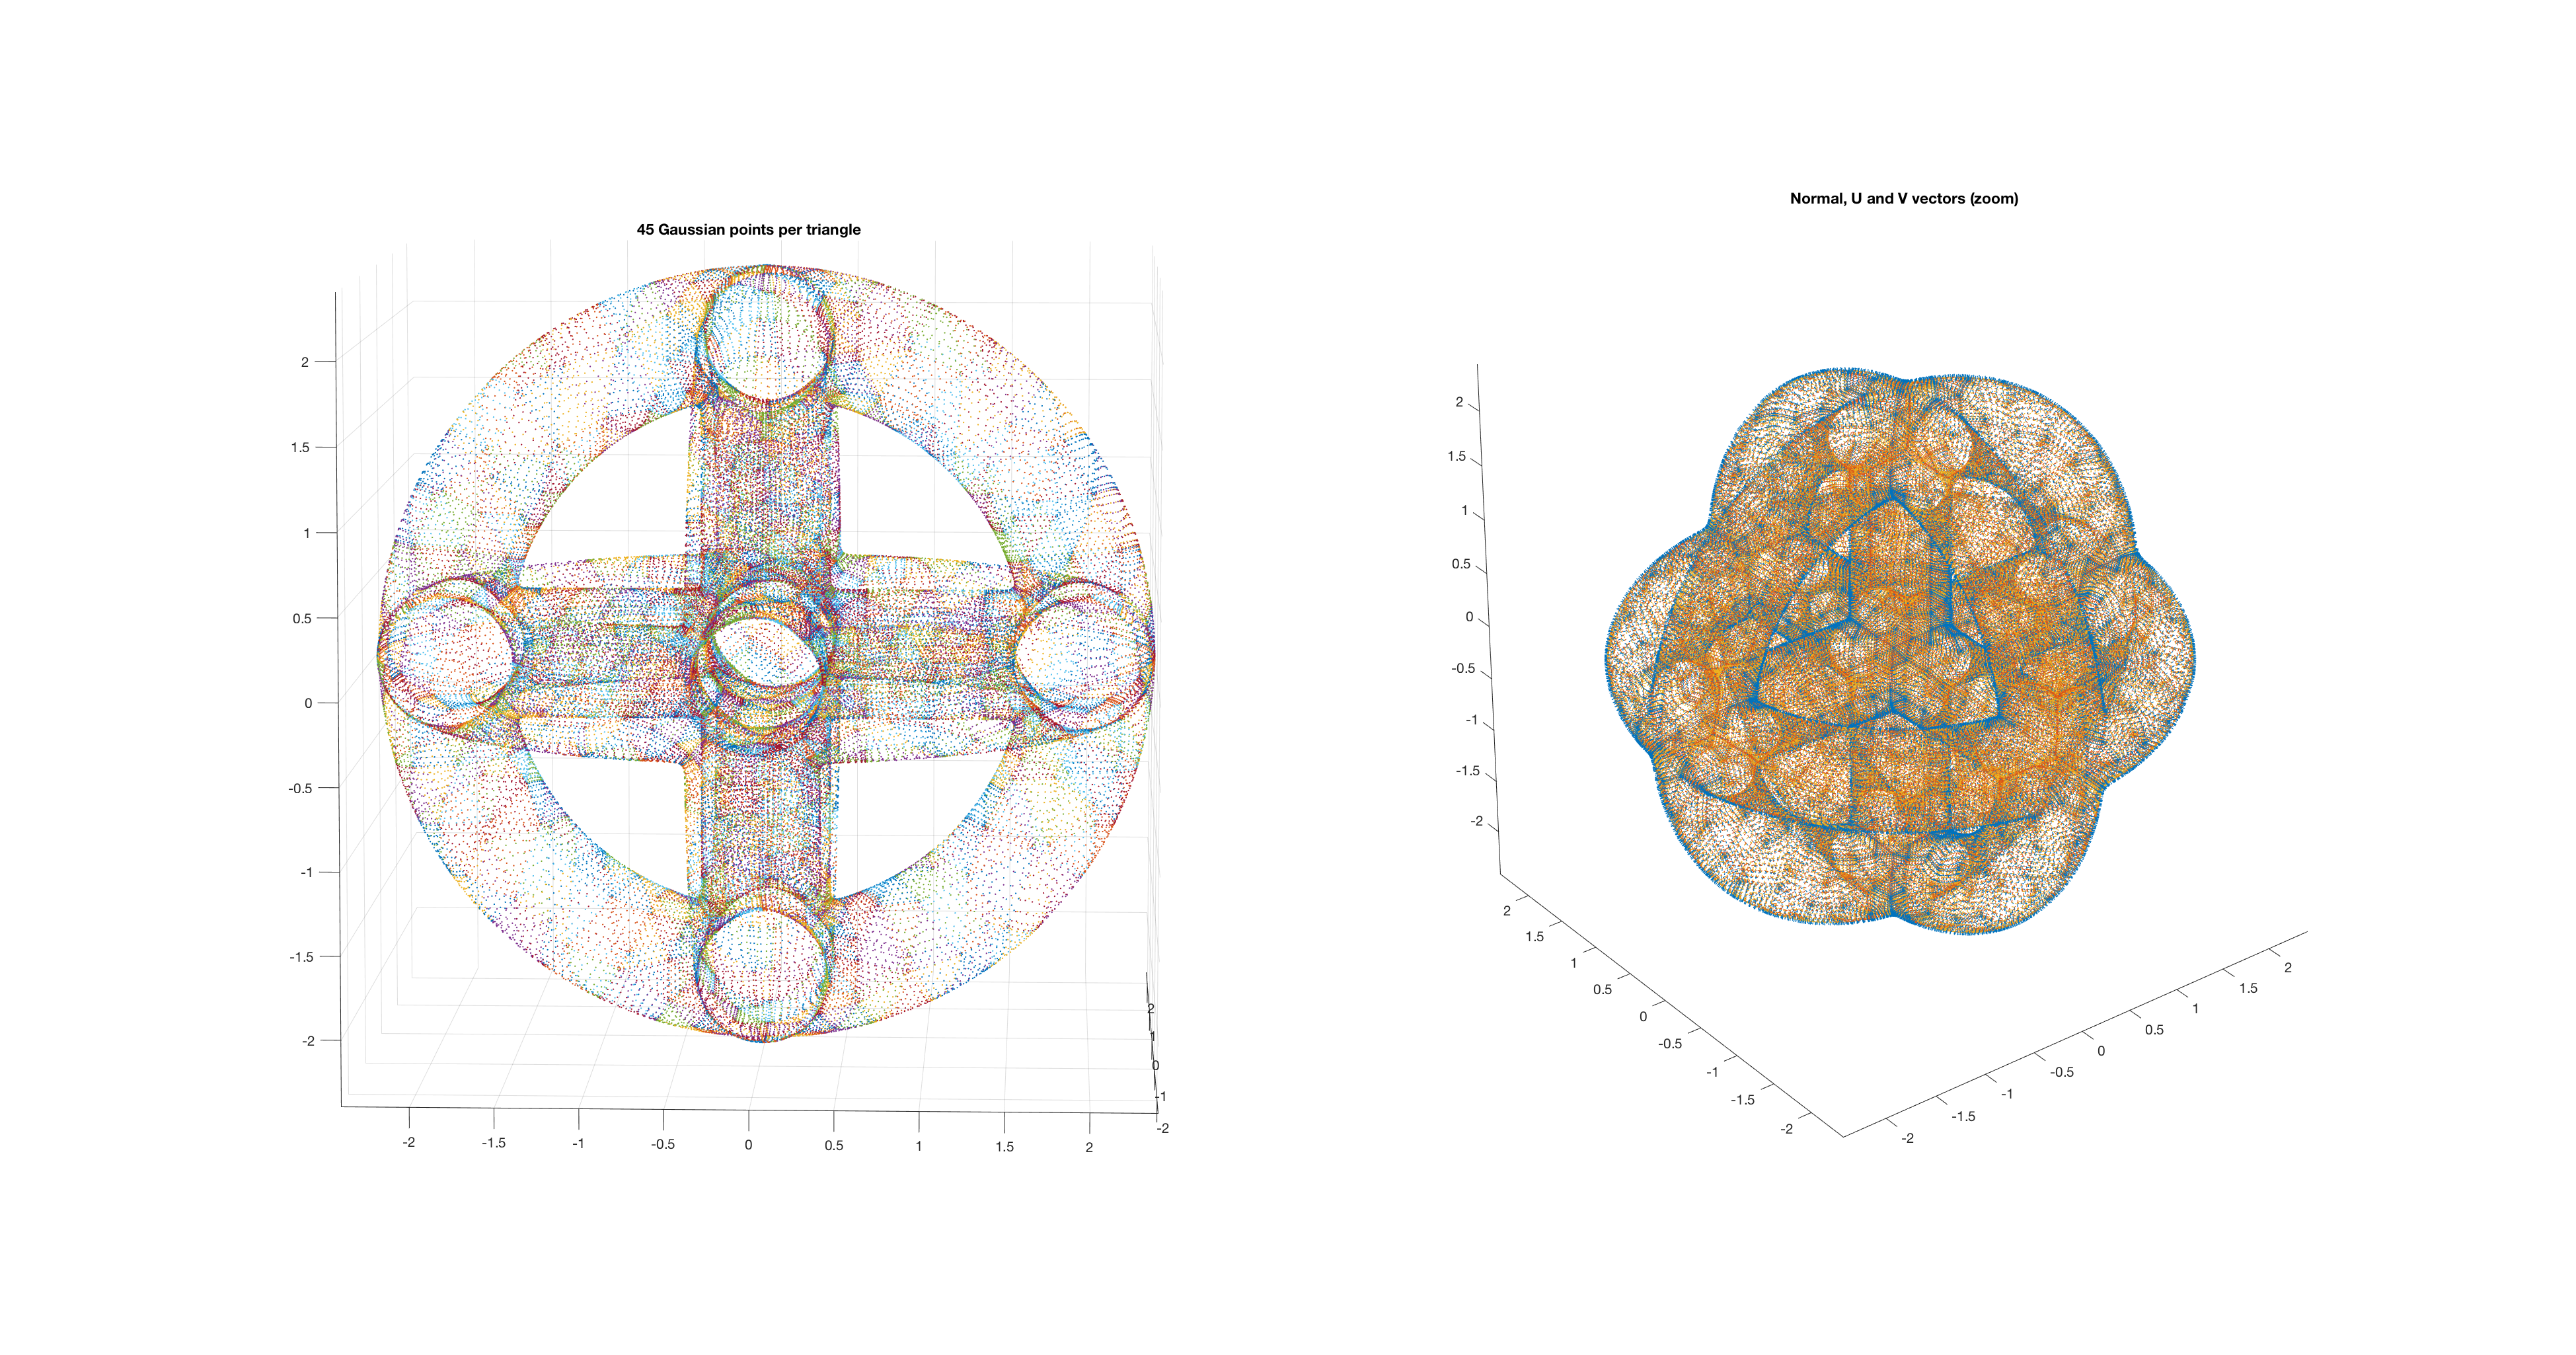
\includegraphics[width=6in]{sci_fi_2.pdf}
\end{center}
\caption{}
\label{sci_fi_2}
\end{figure}

\begin{figure}[H]
\begin{center}
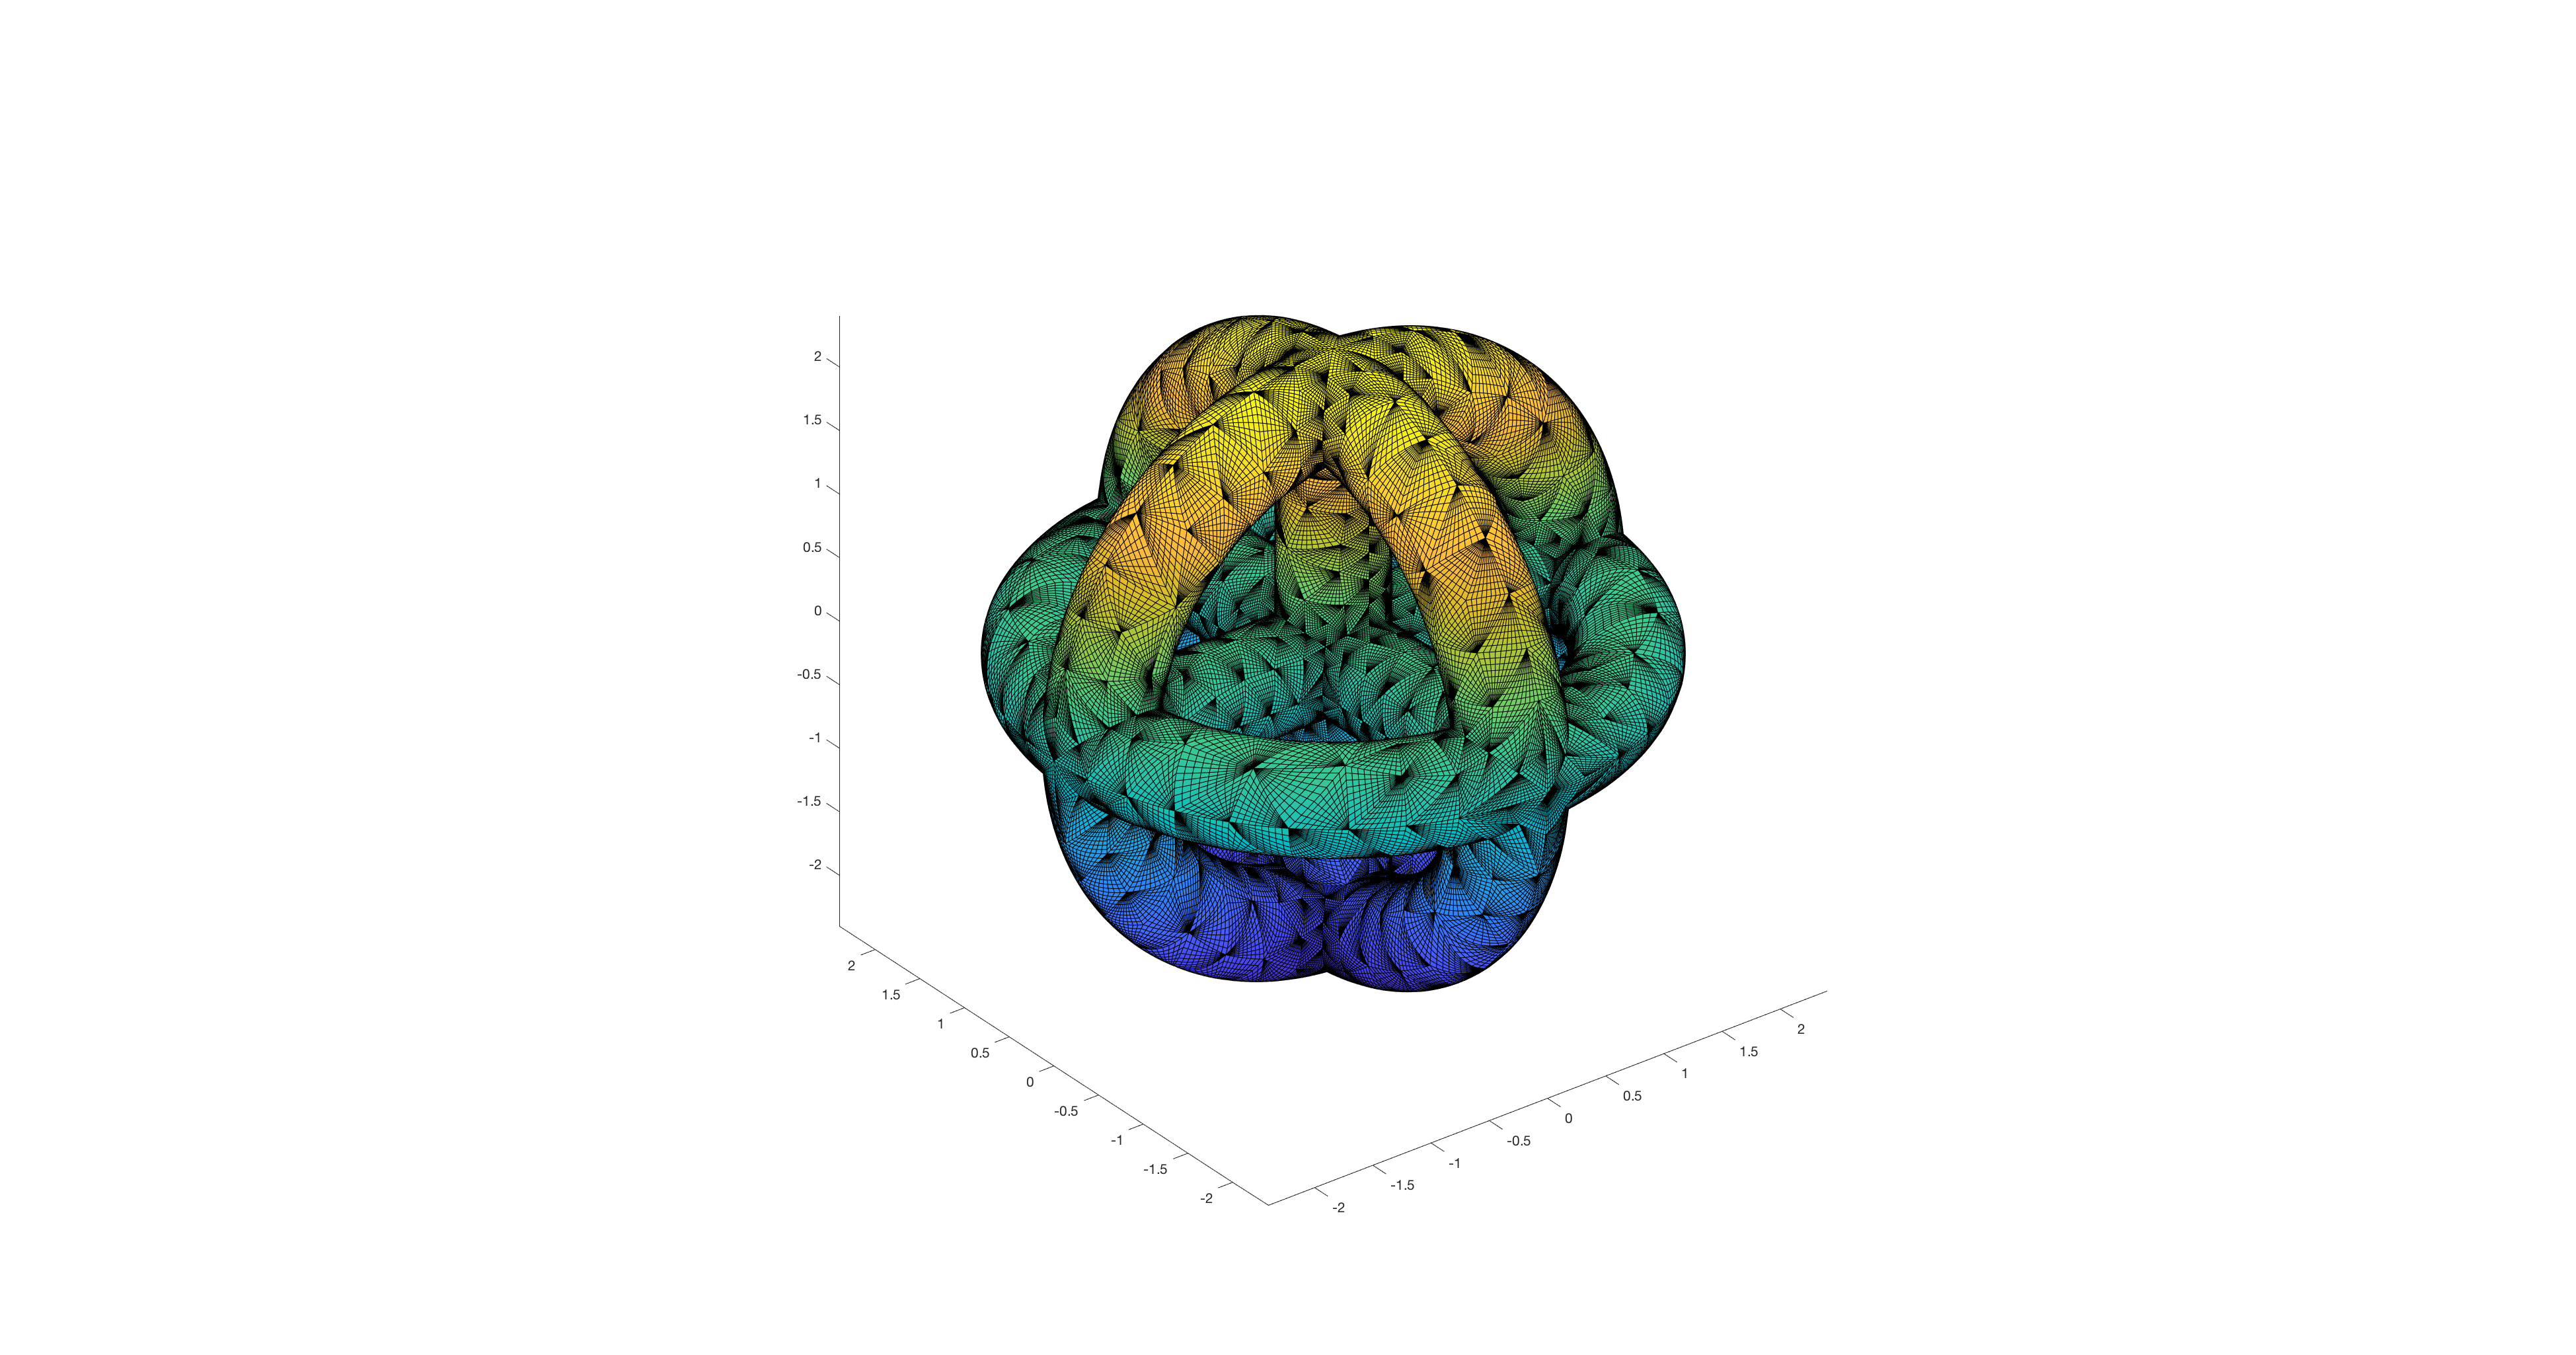
\includegraphics[width=6in]{sci_fi_2_skeleton_view_1.pdf}
\end{center}
\caption{Different view of the skeleton}
\label{sci_fi_2_skeleton_1}
\end{figure}

\begin{figure}[H]
\begin{center}
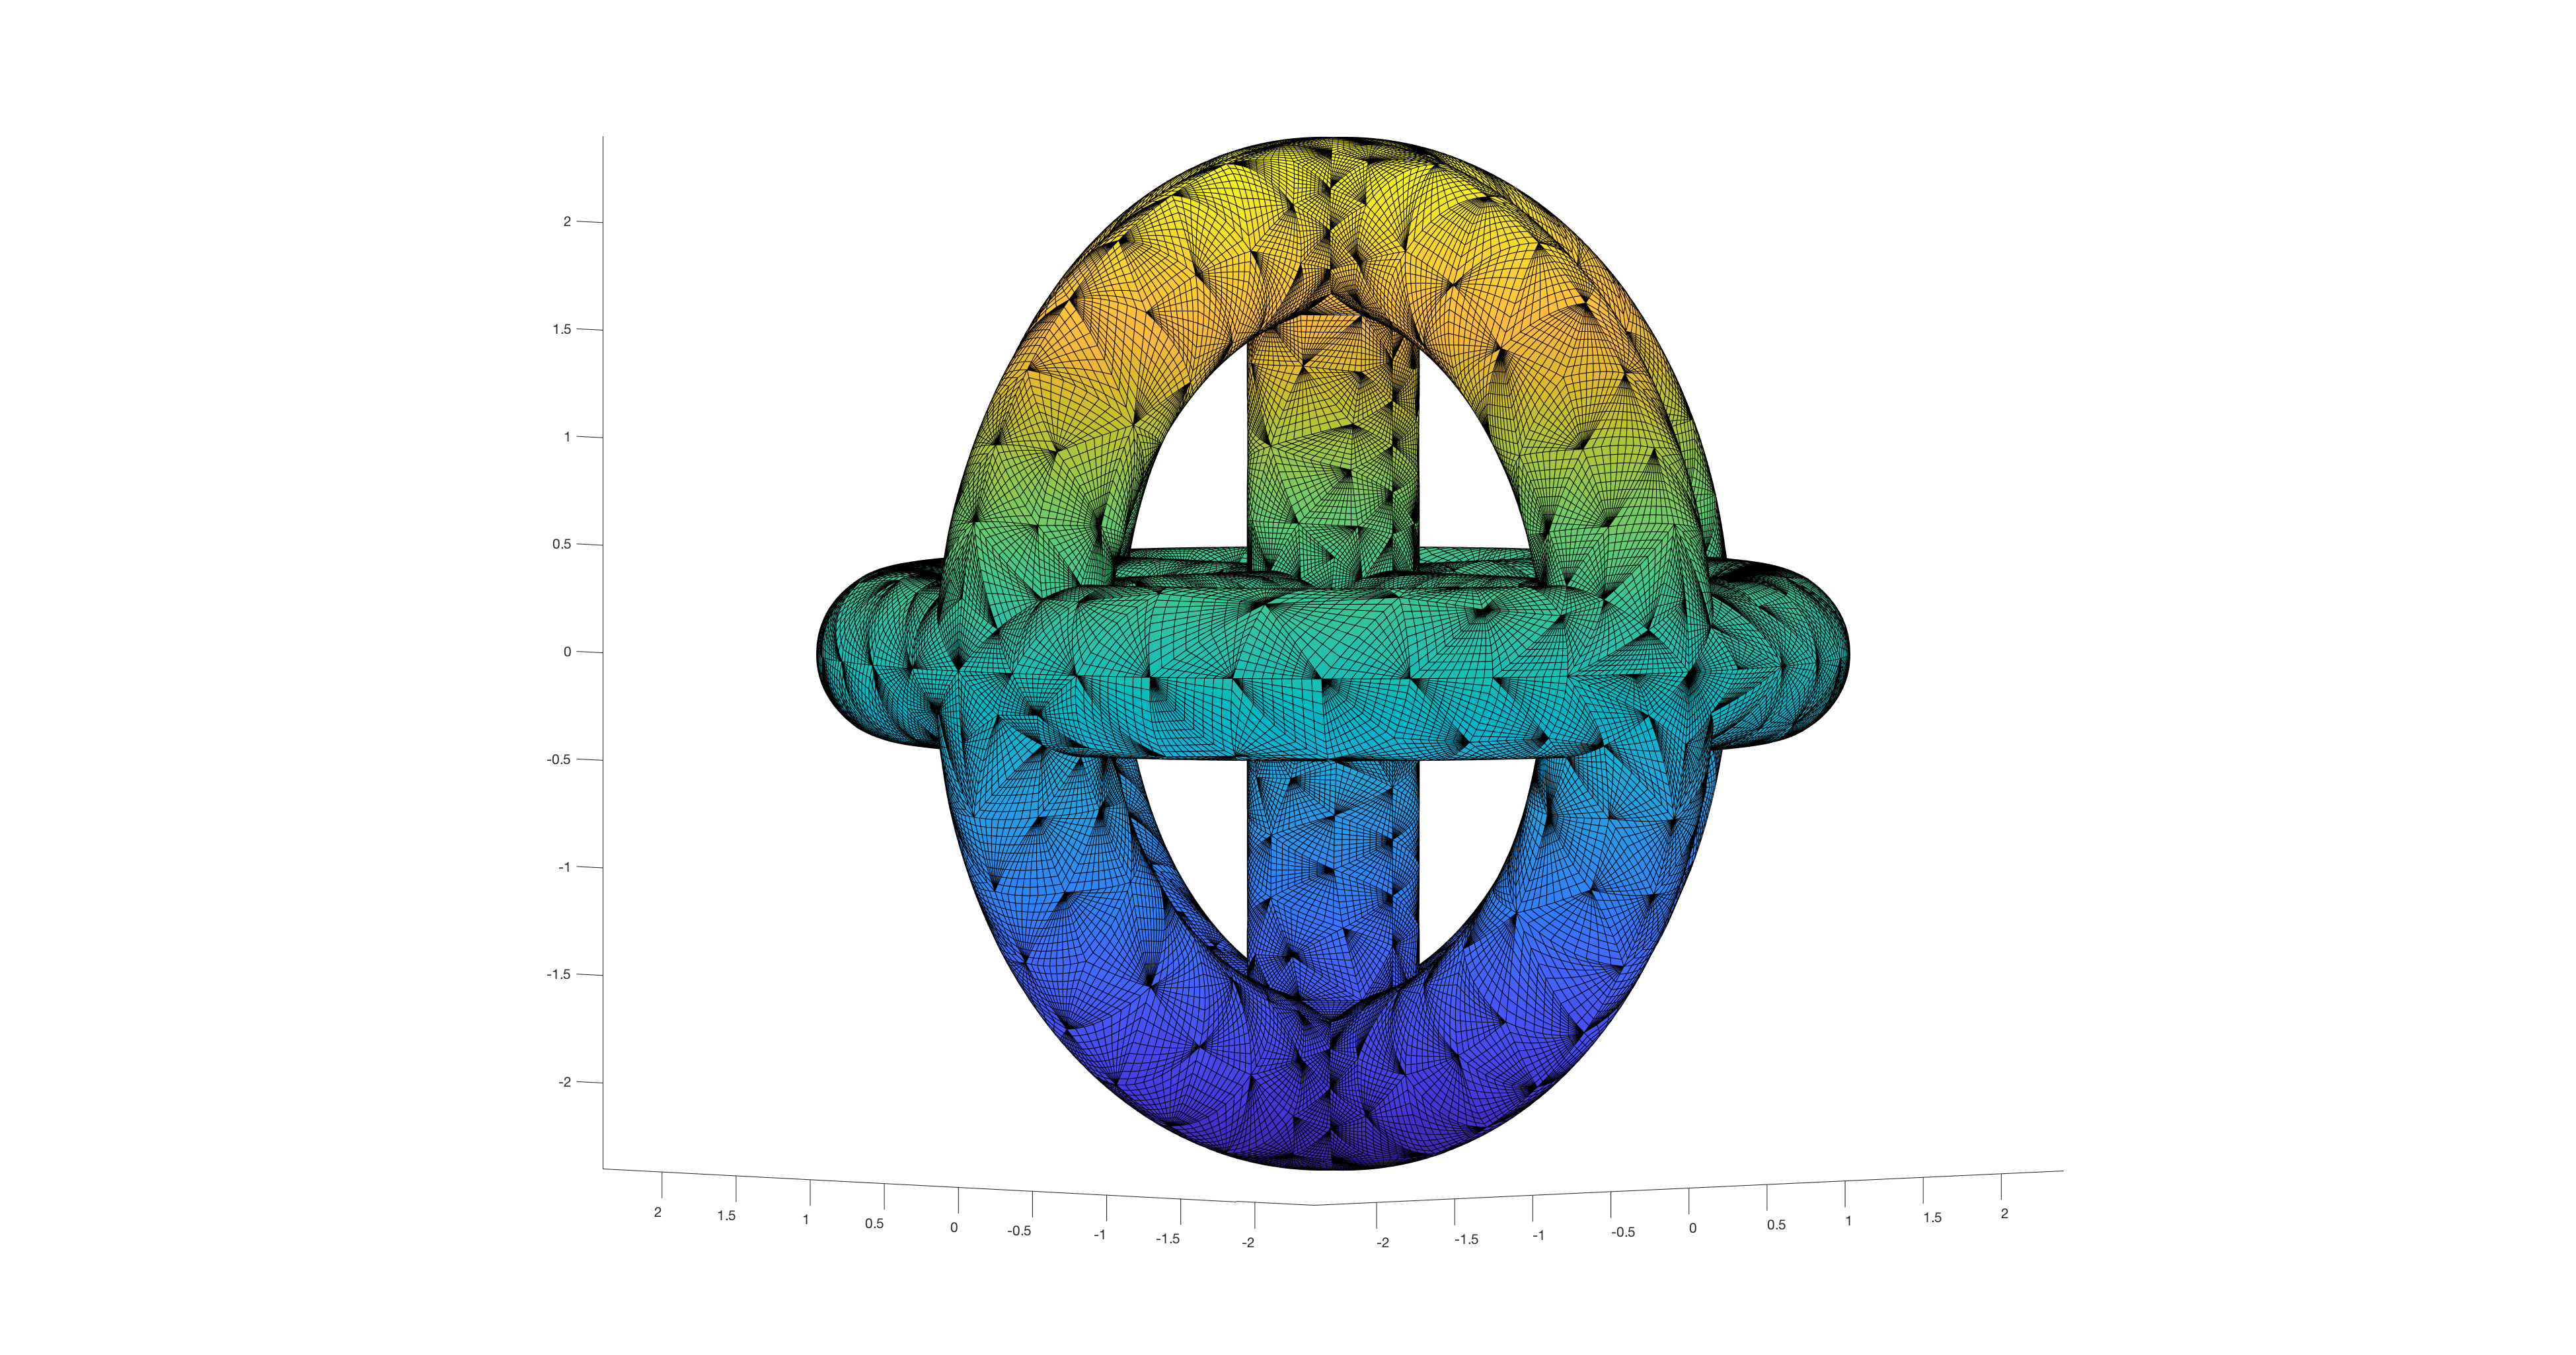
\includegraphics[width=6in]{sci_fi_2_skeleton_view_2.pdf}
\end{center}
\caption{Different view of the skeleton}
\label{sci_fi_2_skeleton_2}
\end{figure}

\begin{figure}[H]
\begin{center}
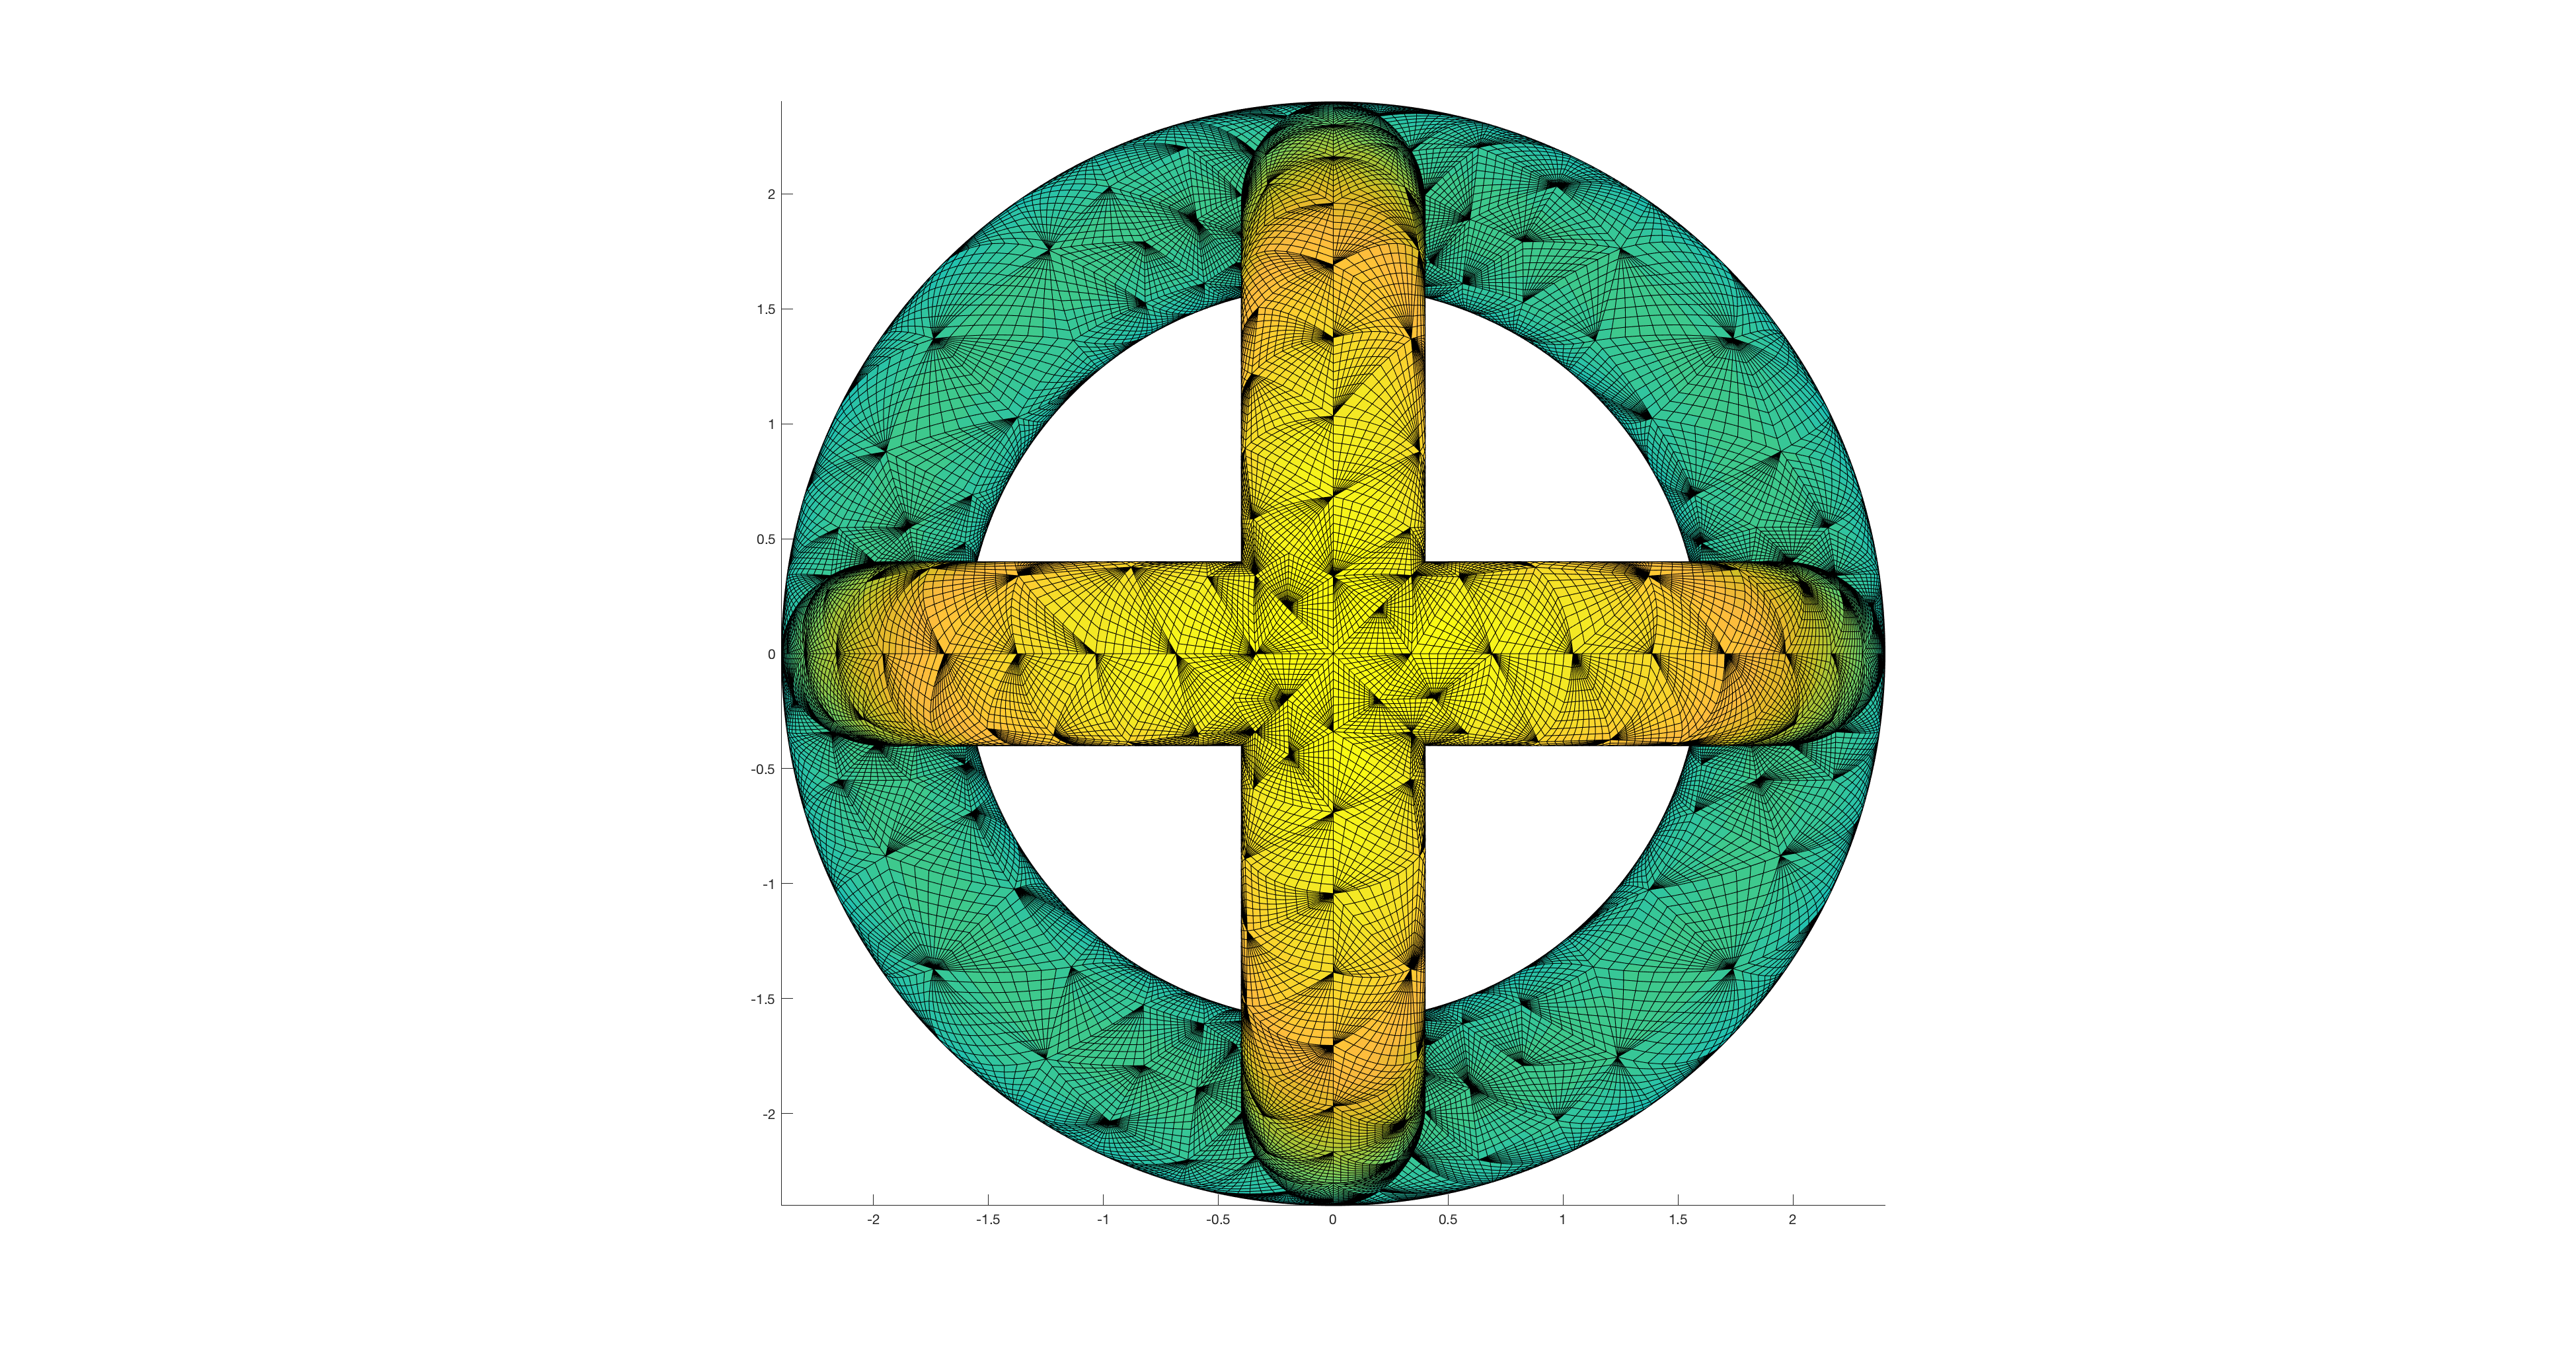
\includegraphics[width=6in]{sci_fi_2_skeleton_view_3.pdf}
\end{center}
\caption{Different view of the skeleton}
\label{sci_fi_2_skeleton_3}
\end{figure}

\begin{figure}[H]
\begin{center}
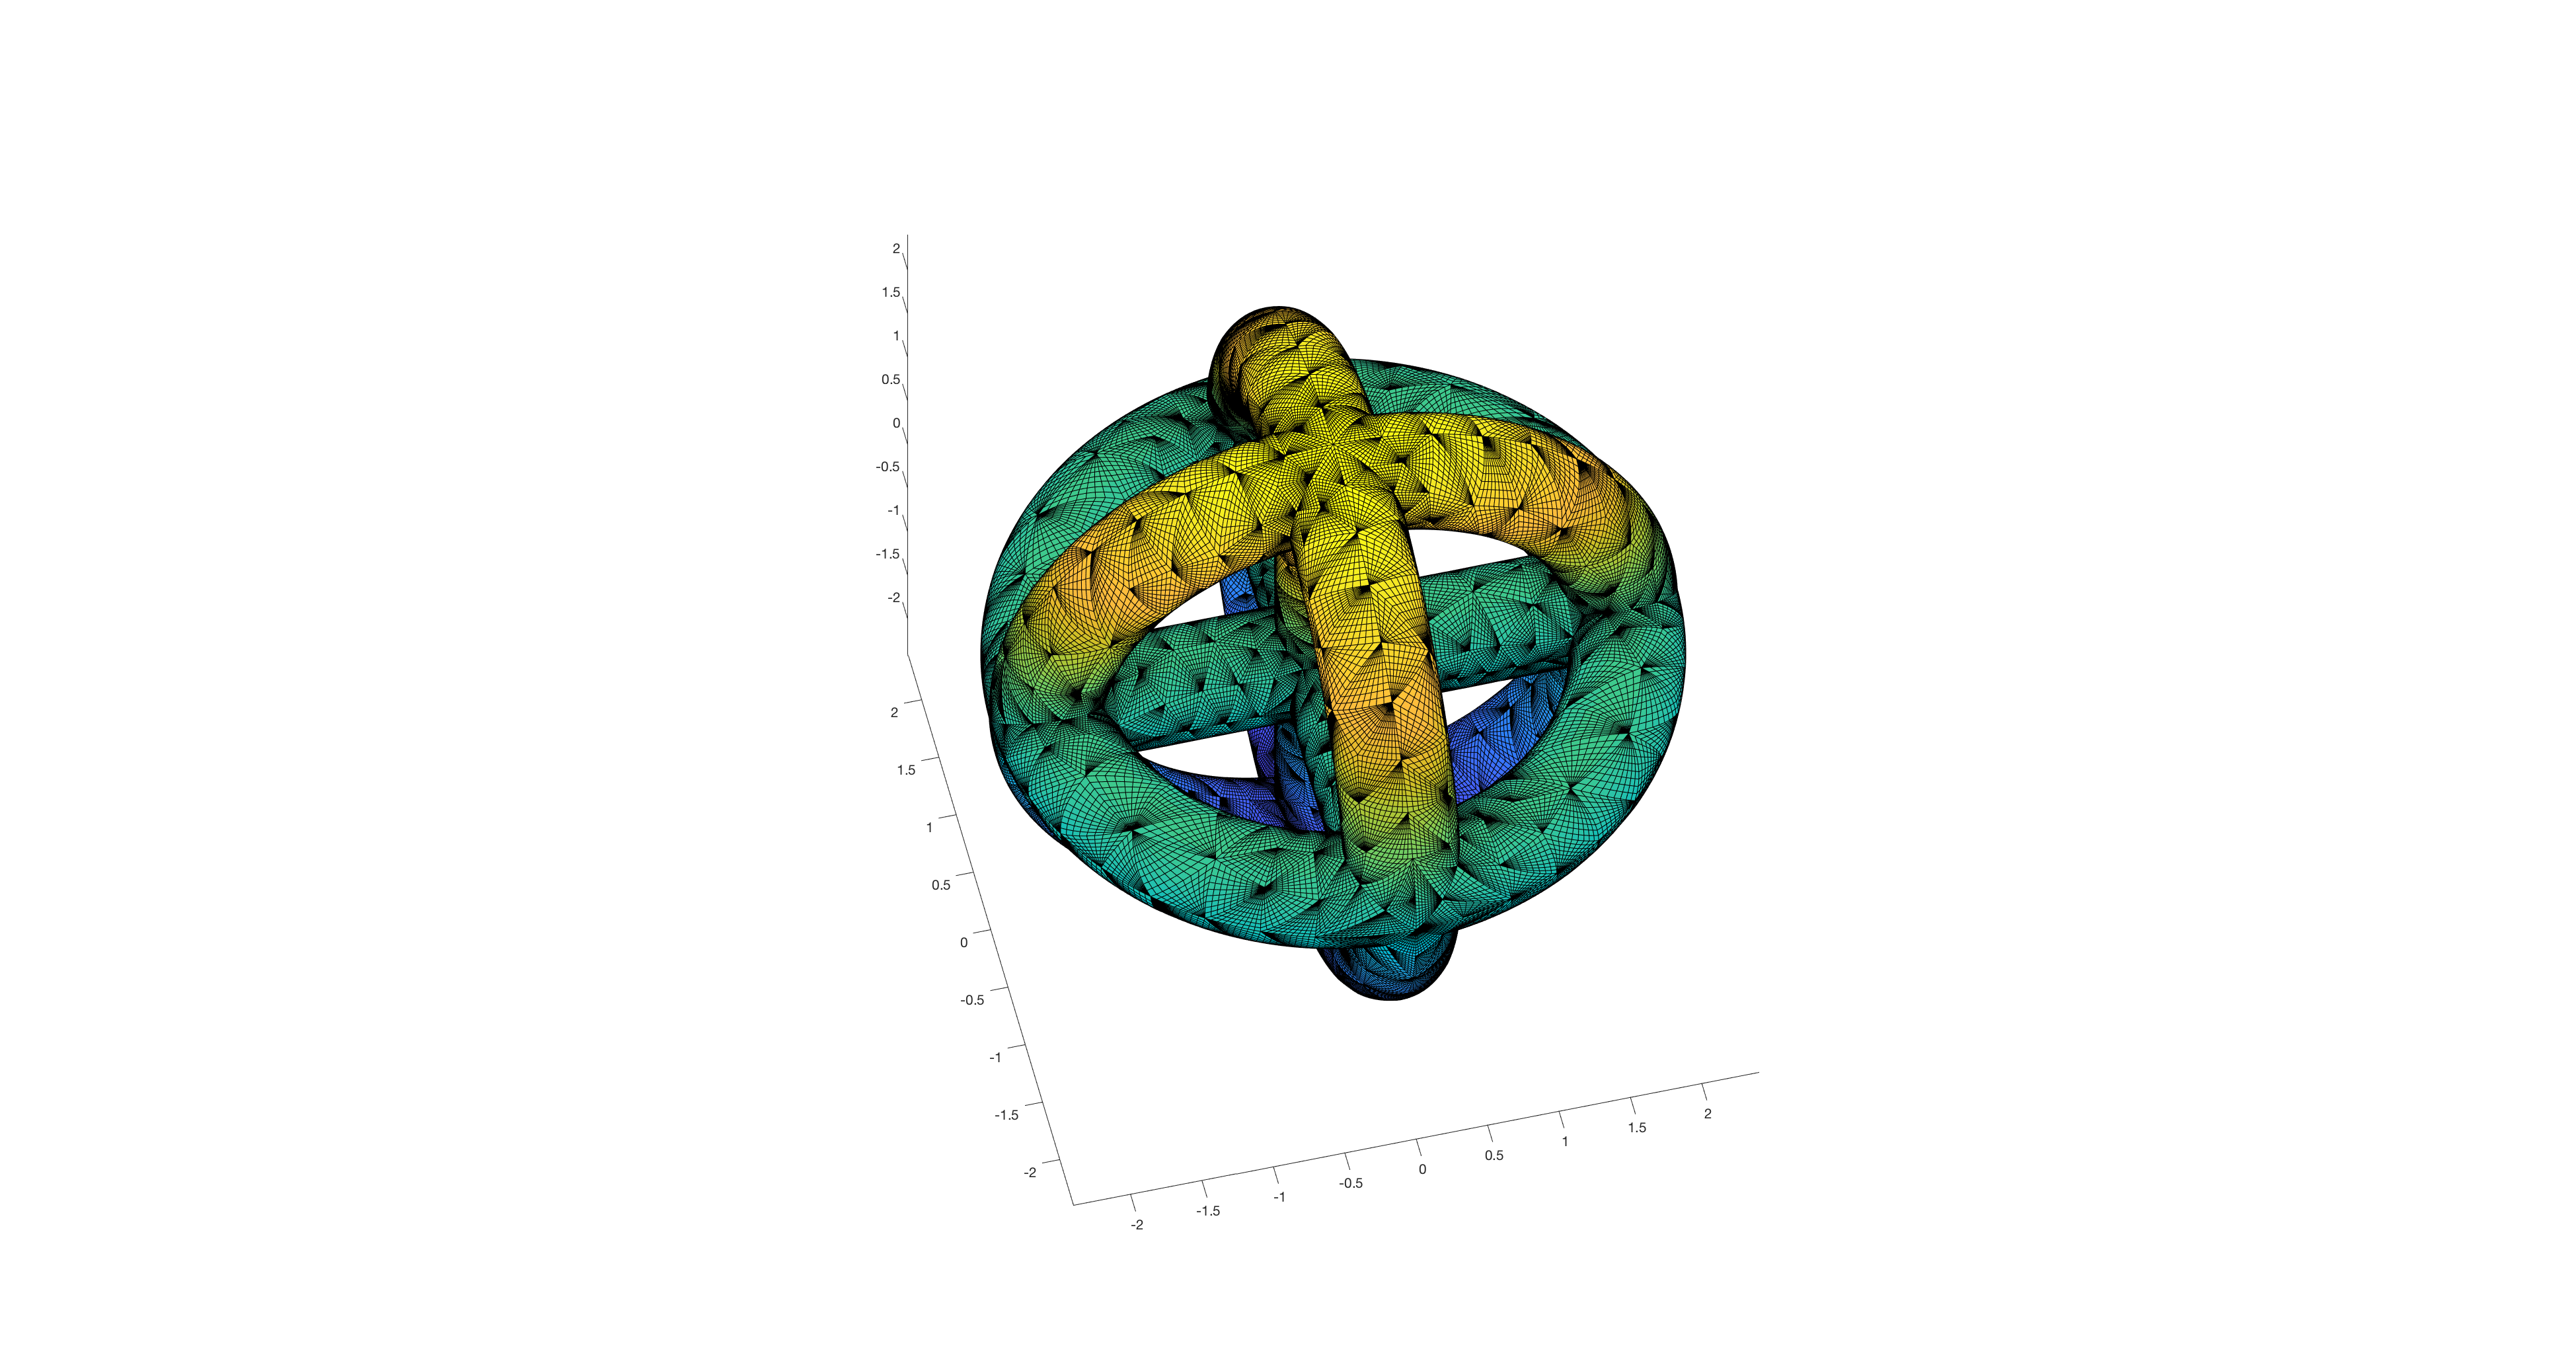
\includegraphics[width=6in]{sci_fi_2_skeleton_view_4.pdf}
\end{center}
\caption{Different view of the skeleton}
\label{sci_fi_2_skeleton_4}
\end{figure}





\newpage
\subsection{open\_cavity\_30deg\_v2.msh (adaptive\_flag=0)}
Open cavity. Standard challenging problem for high frequency EM scattering. No refinement study yet, accuracy obtained for $n_{refinement}=0$ and n\_order\_sf=45 is $Err=6.3\cdot 10^{-6}$
\begin{figure}[H]
\begin{center}
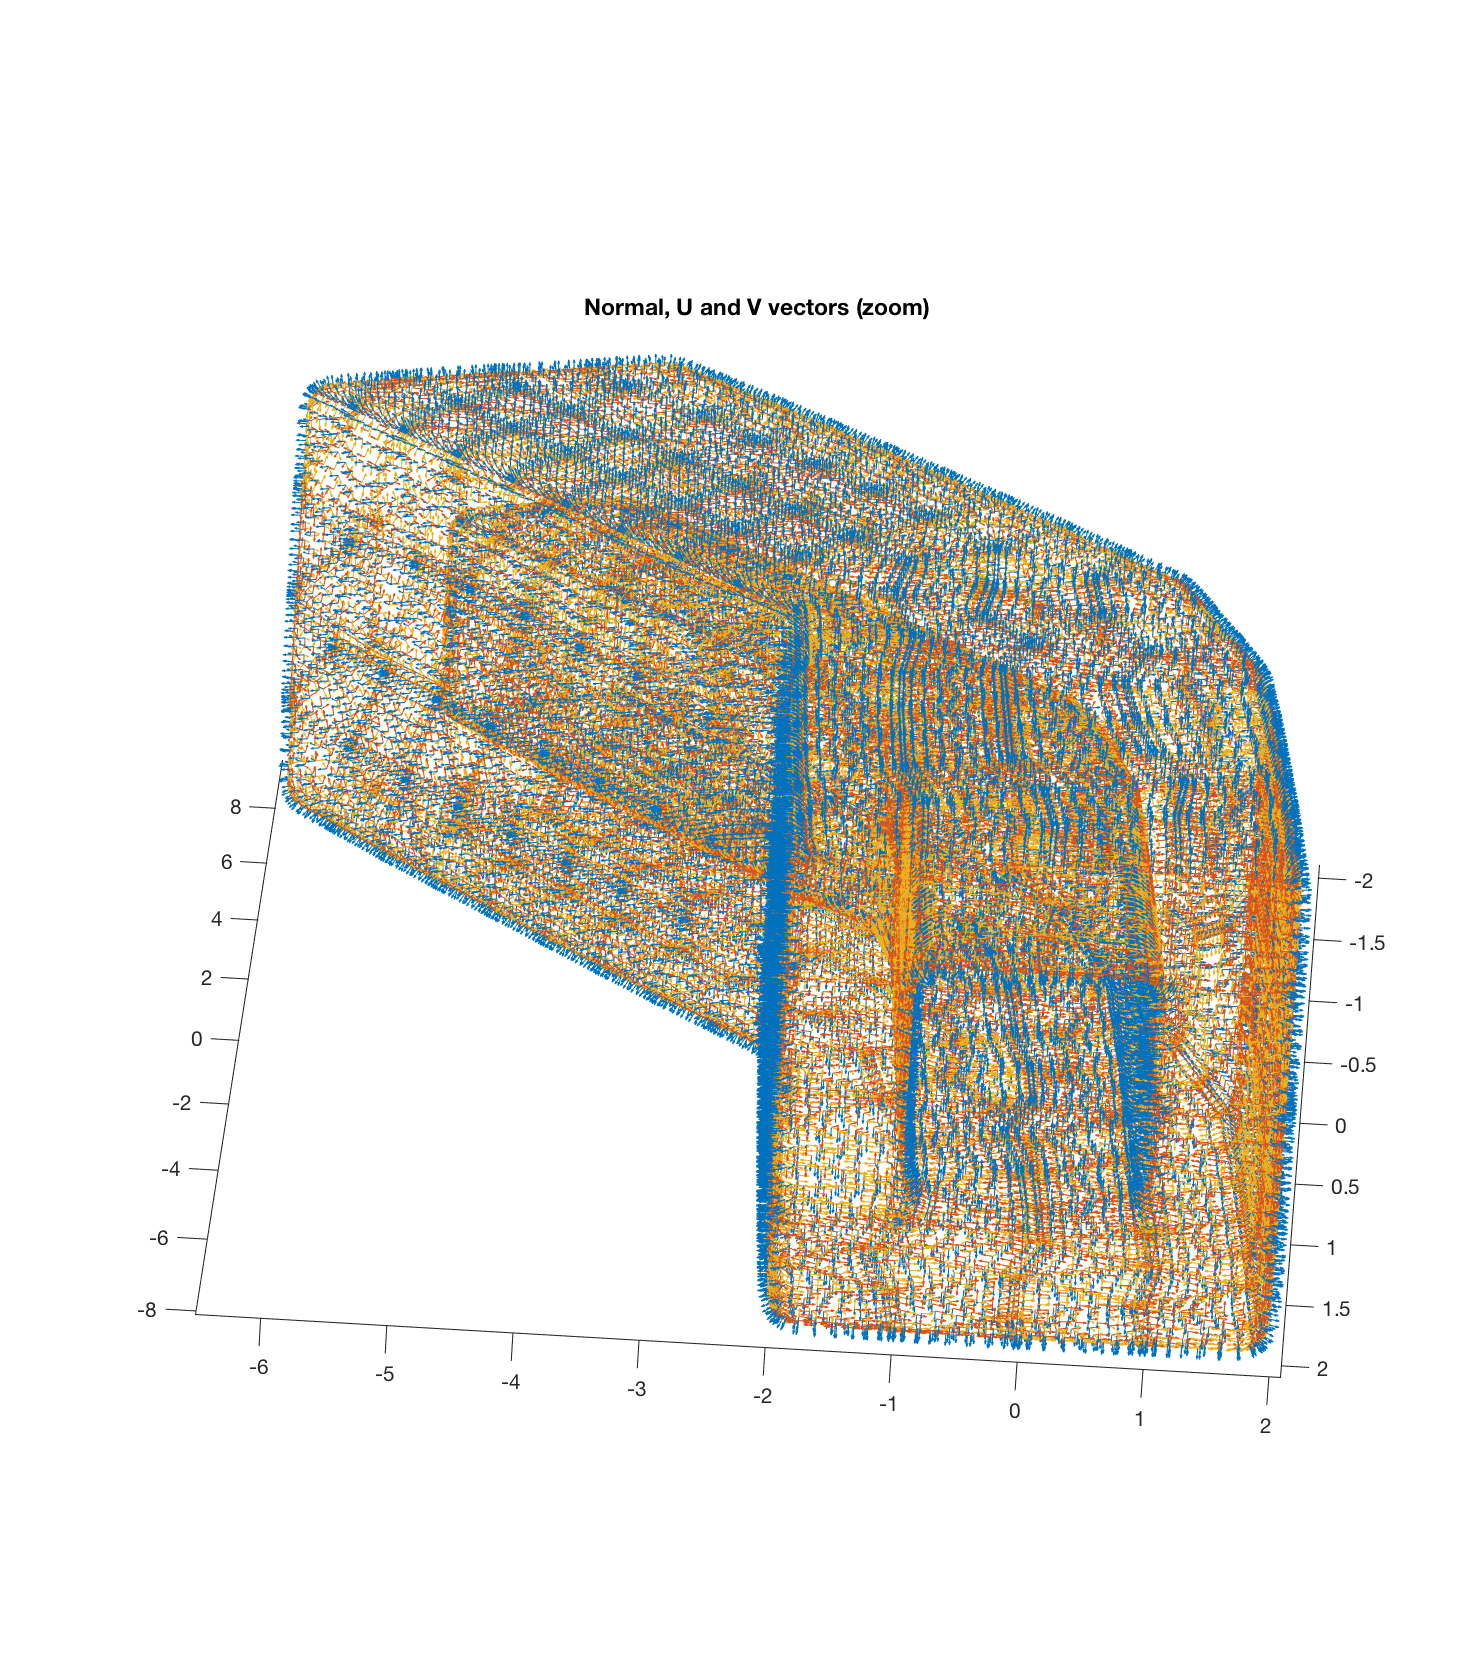
\includegraphics[width=5.5in]{open_cavity_basis.pdf}
\end{center}
\caption{}
\label{open_cavity_basis}
\end{figure}

\begin{figure}[H]
\begin{center}
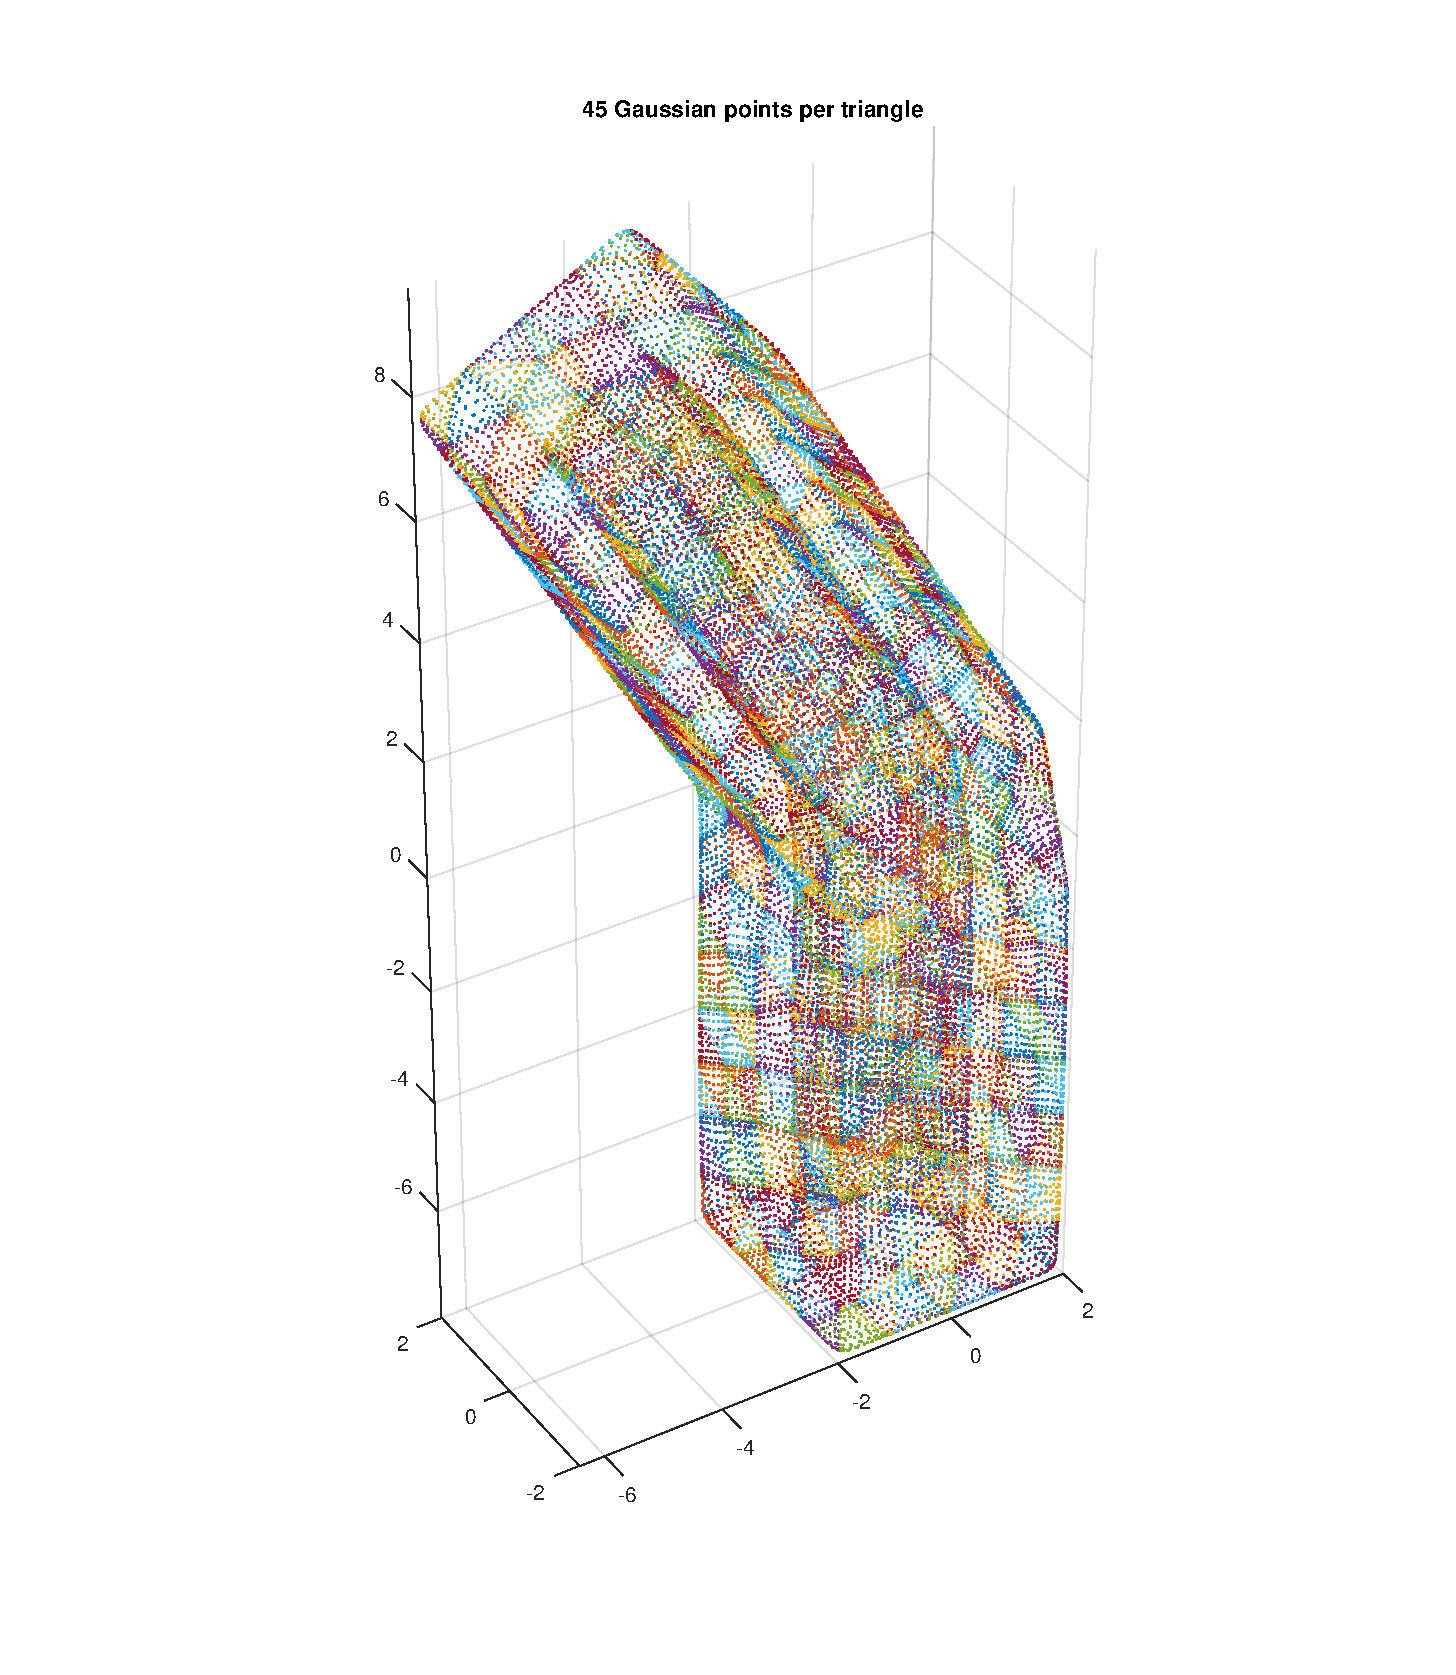
\includegraphics[width=6in]{open_cavity_points.pdf}
\end{center}
\caption{}
\label{open_cavity_points}
\end{figure}

\begin{figure}[H]
\begin{center}
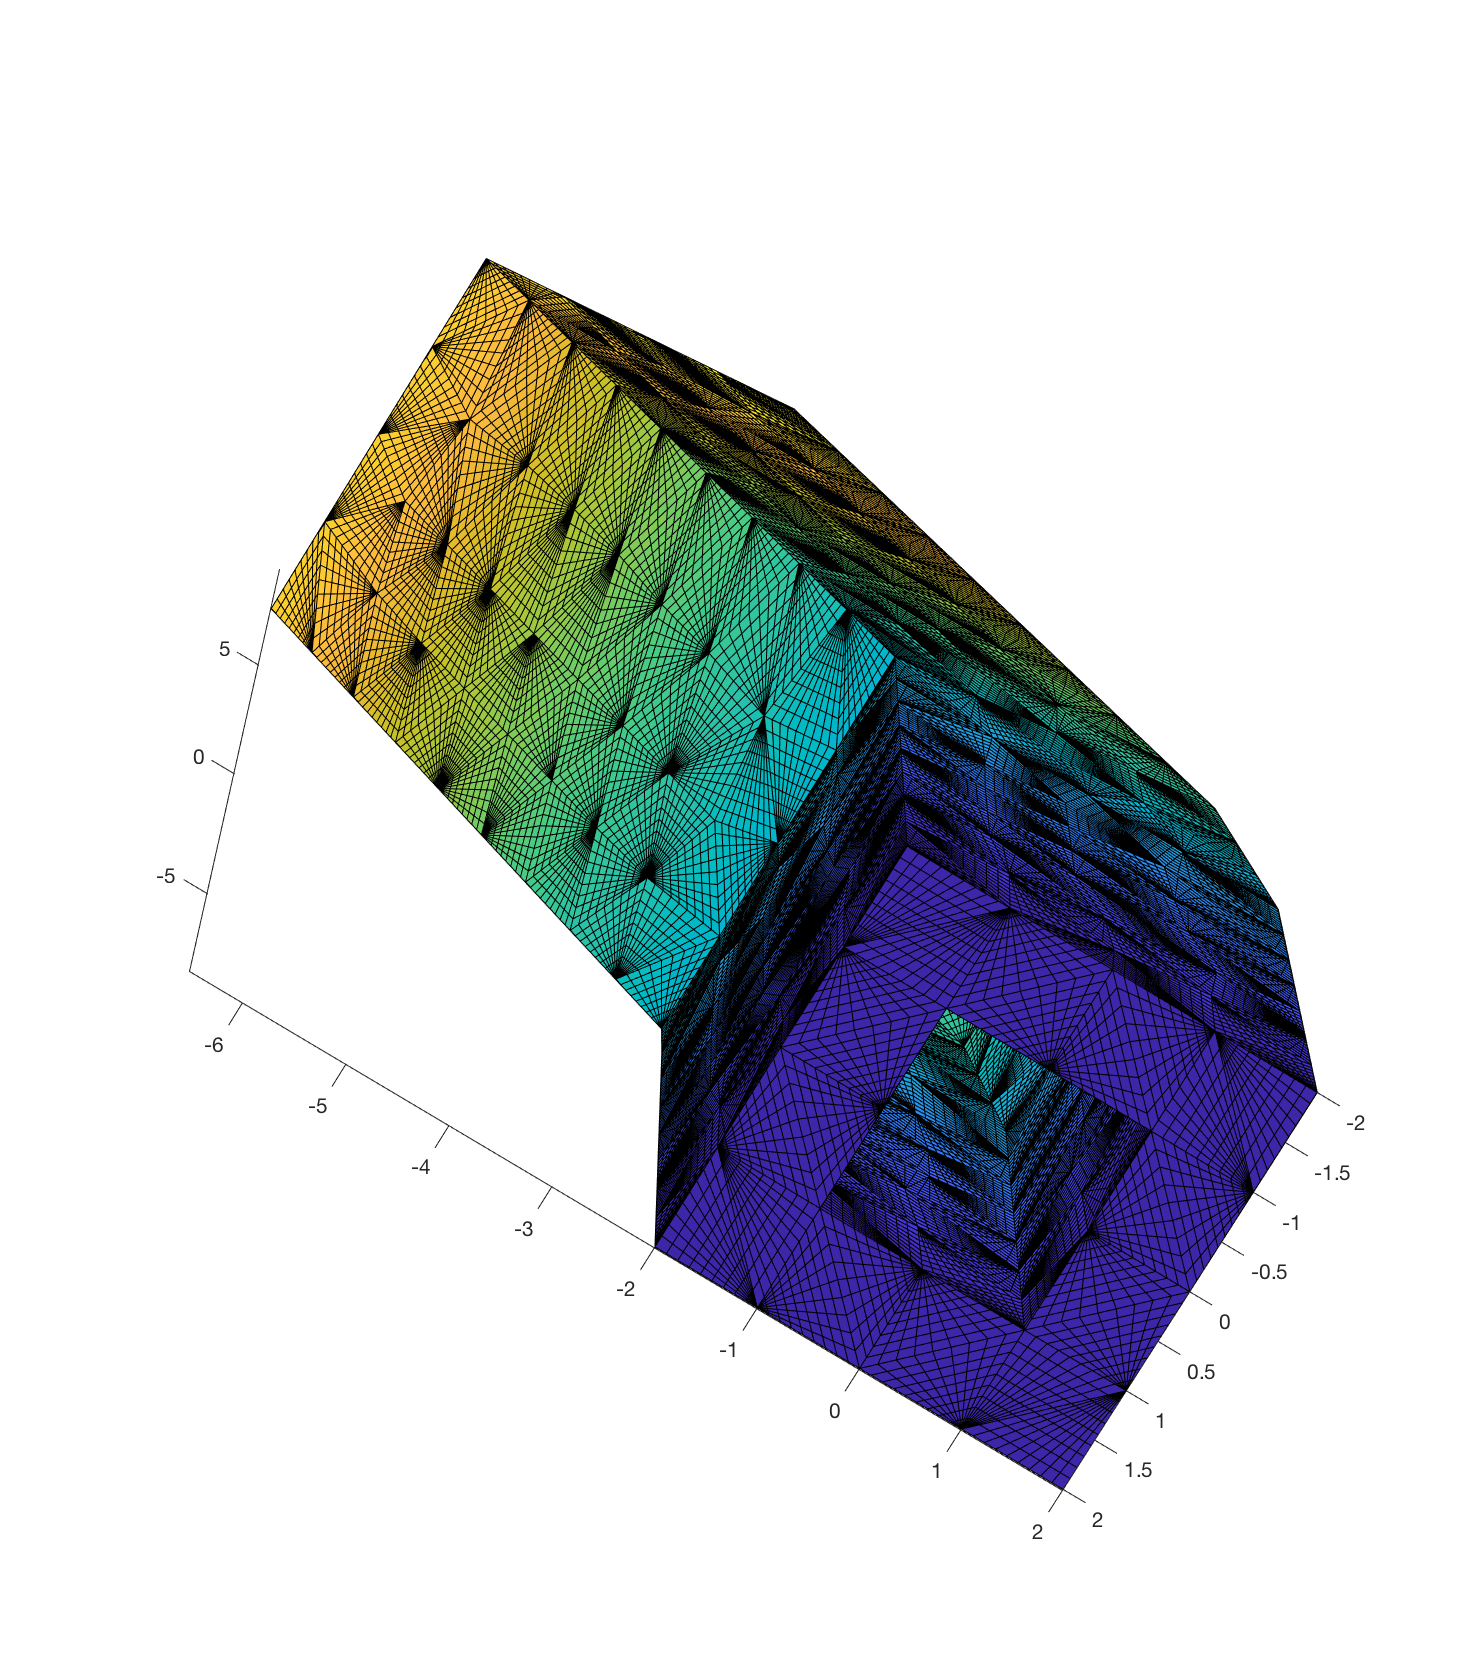
\includegraphics[width=6in]{open_cavity_skeleton.pdf}
\end{center}
\caption{View of the skeleton used for the open cavity}
\label{open_cavity_skeleton}
\end{figure}

\begin{figure}[H]
\begin{center}
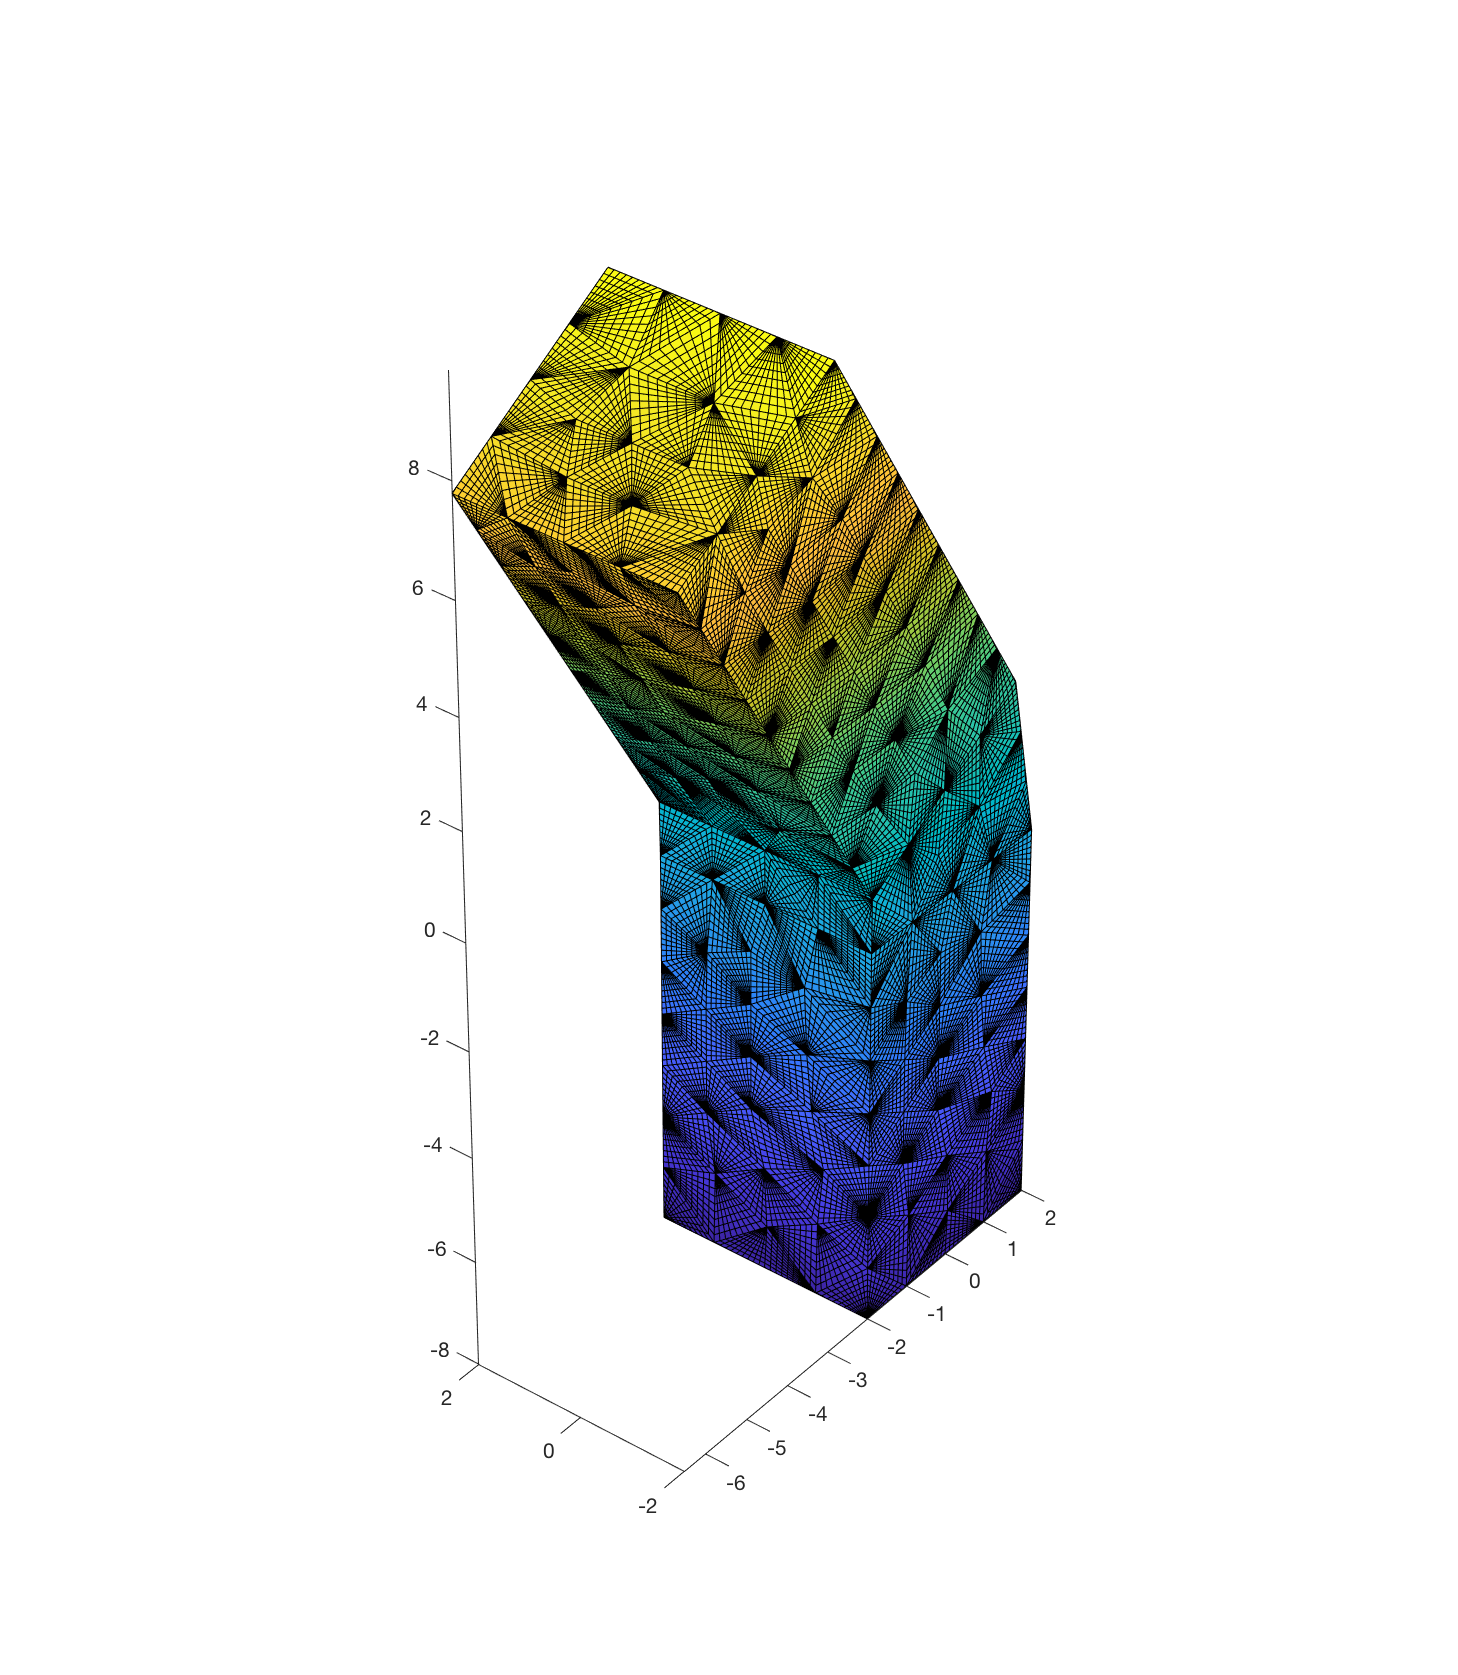
\includegraphics[width=6in]{open_cavity_skeleton_2.pdf}
\end{center}
\caption{View of the skeleton used for the open cavity}
\label{open_cavity_skeleton}
\end{figure}




\newpage
\subsection{parabolic\_antenna.msh (adaptive\_flag=1)}
Parabolic reflector with support for a small feed antenna at its focus. Same geometry inserted in the warship (last example). No refinement study yet, accuracy obtained for $n_{refinement}=0$ and n\_order\_sf=45 is $Err=4.8\cdot 10^{-6}$
\begin{figure}[H]
\begin{center}
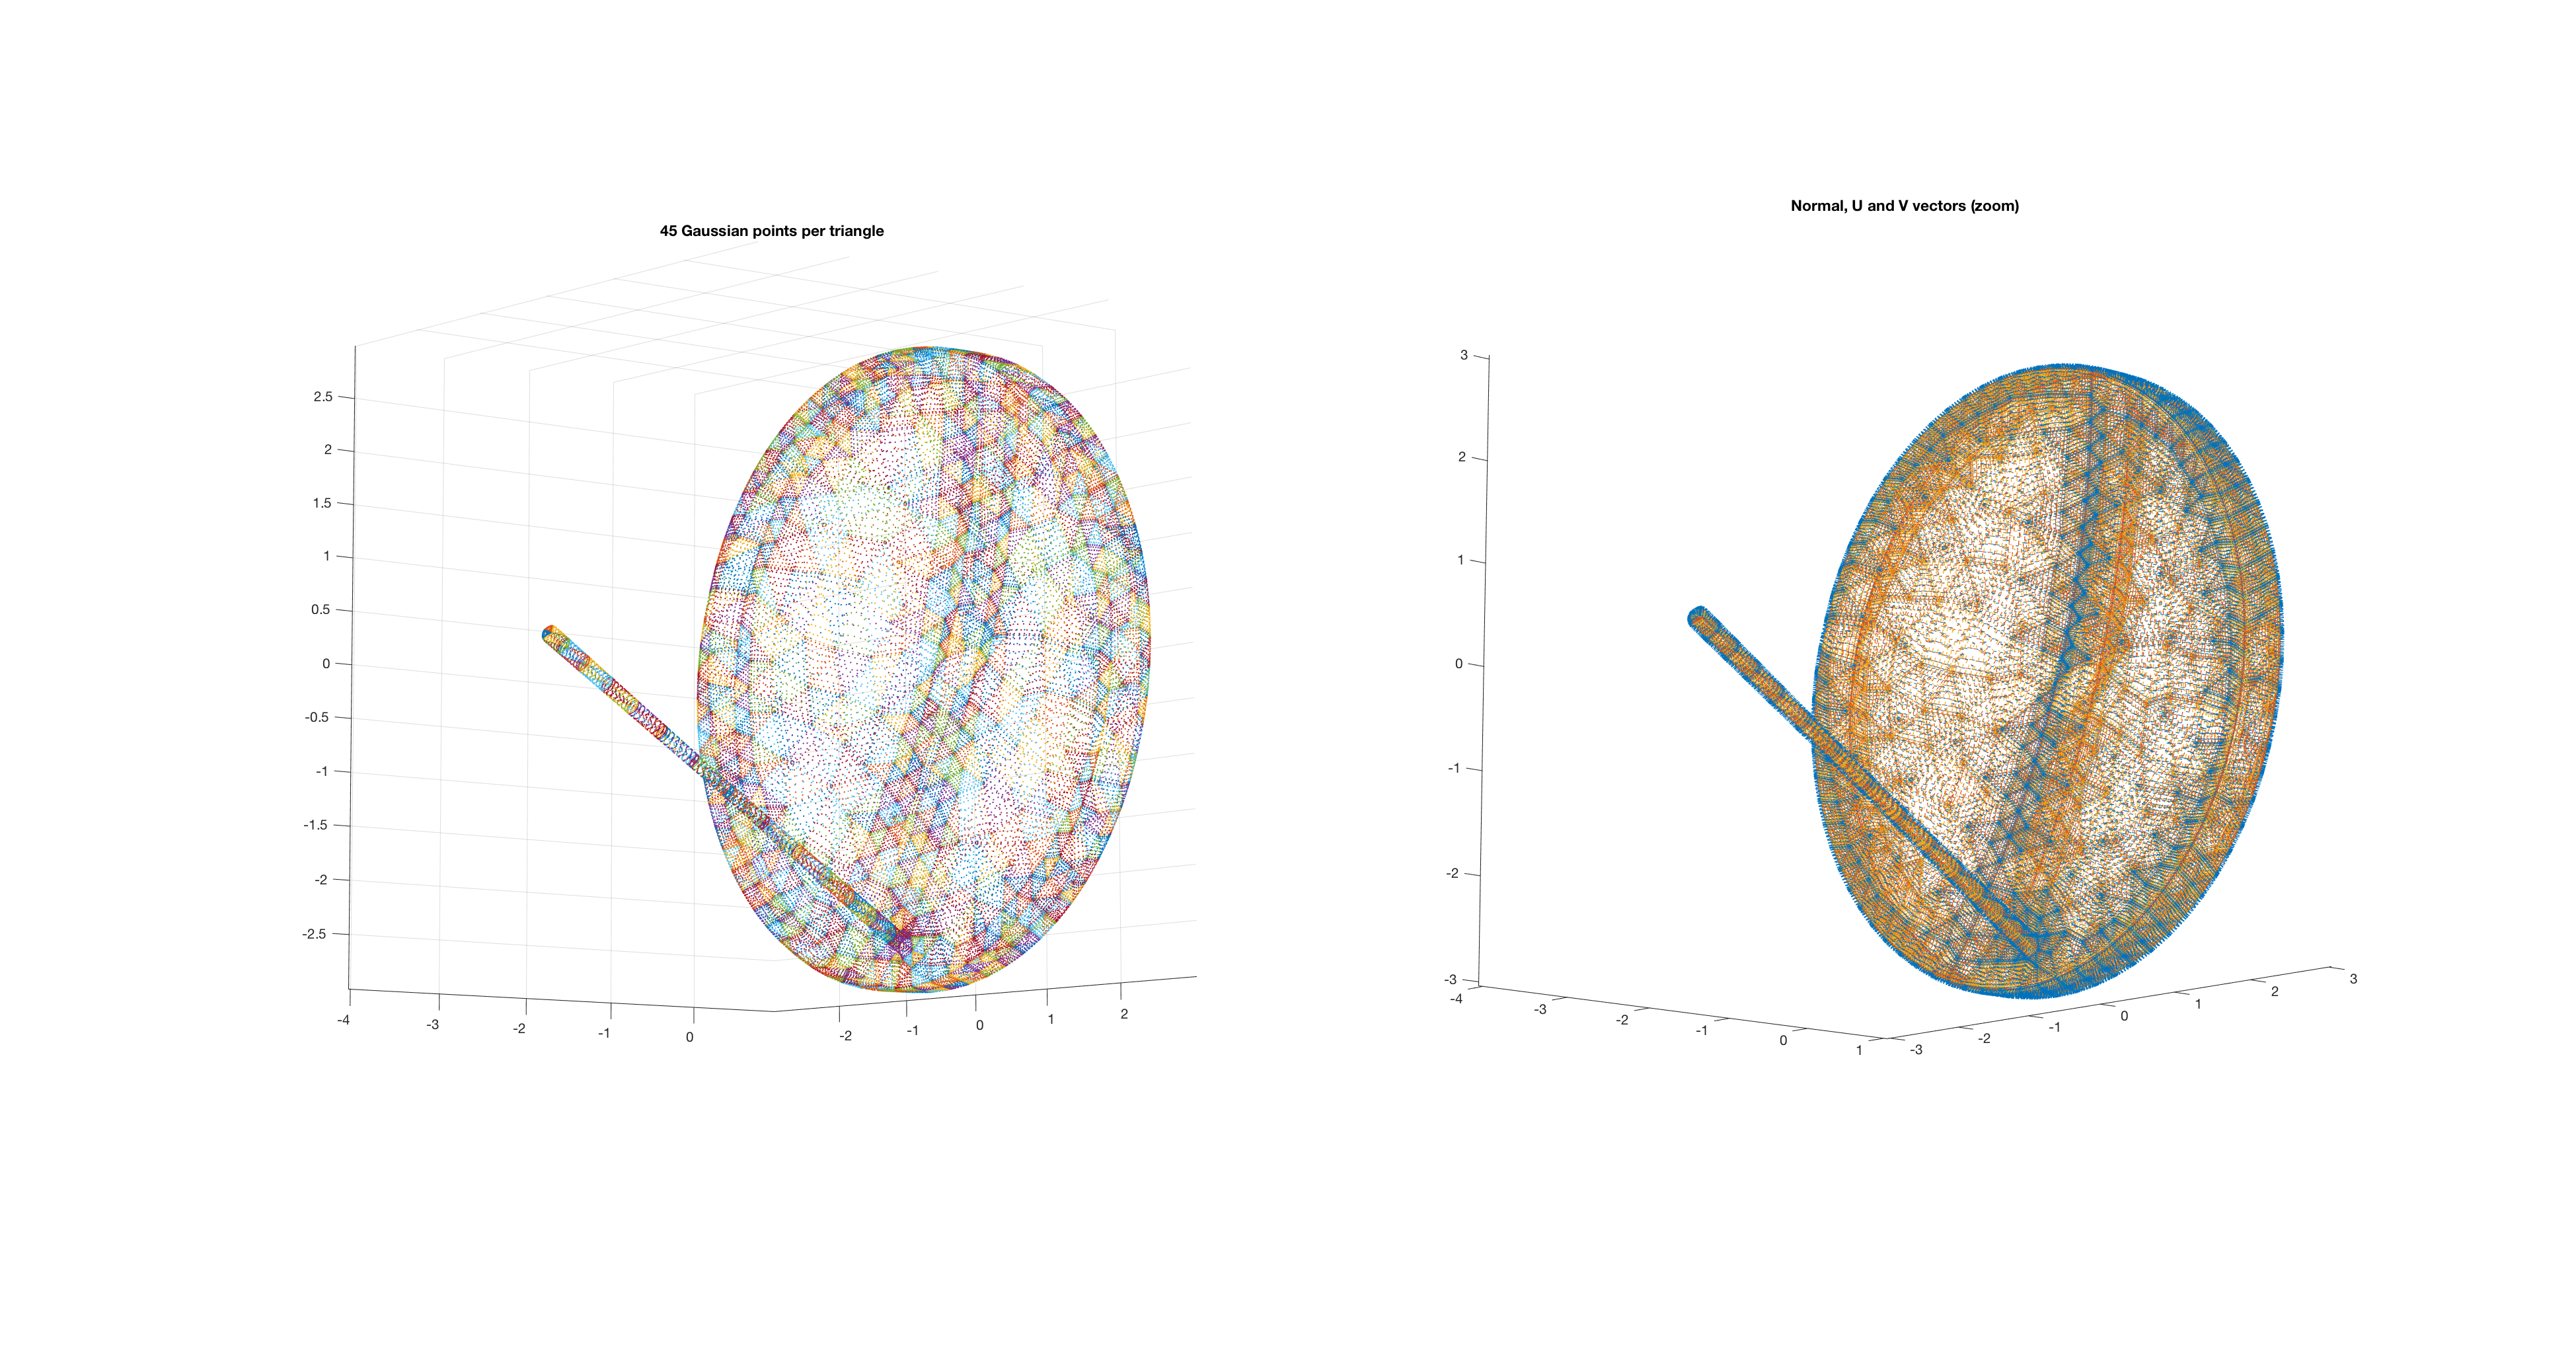
\includegraphics[width=6in]{parabolic_antenna.pdf}
\end{center}
\caption{}
\label{parabolic_antenna}
\end{figure}

\begin{figure}[H]
\begin{center}
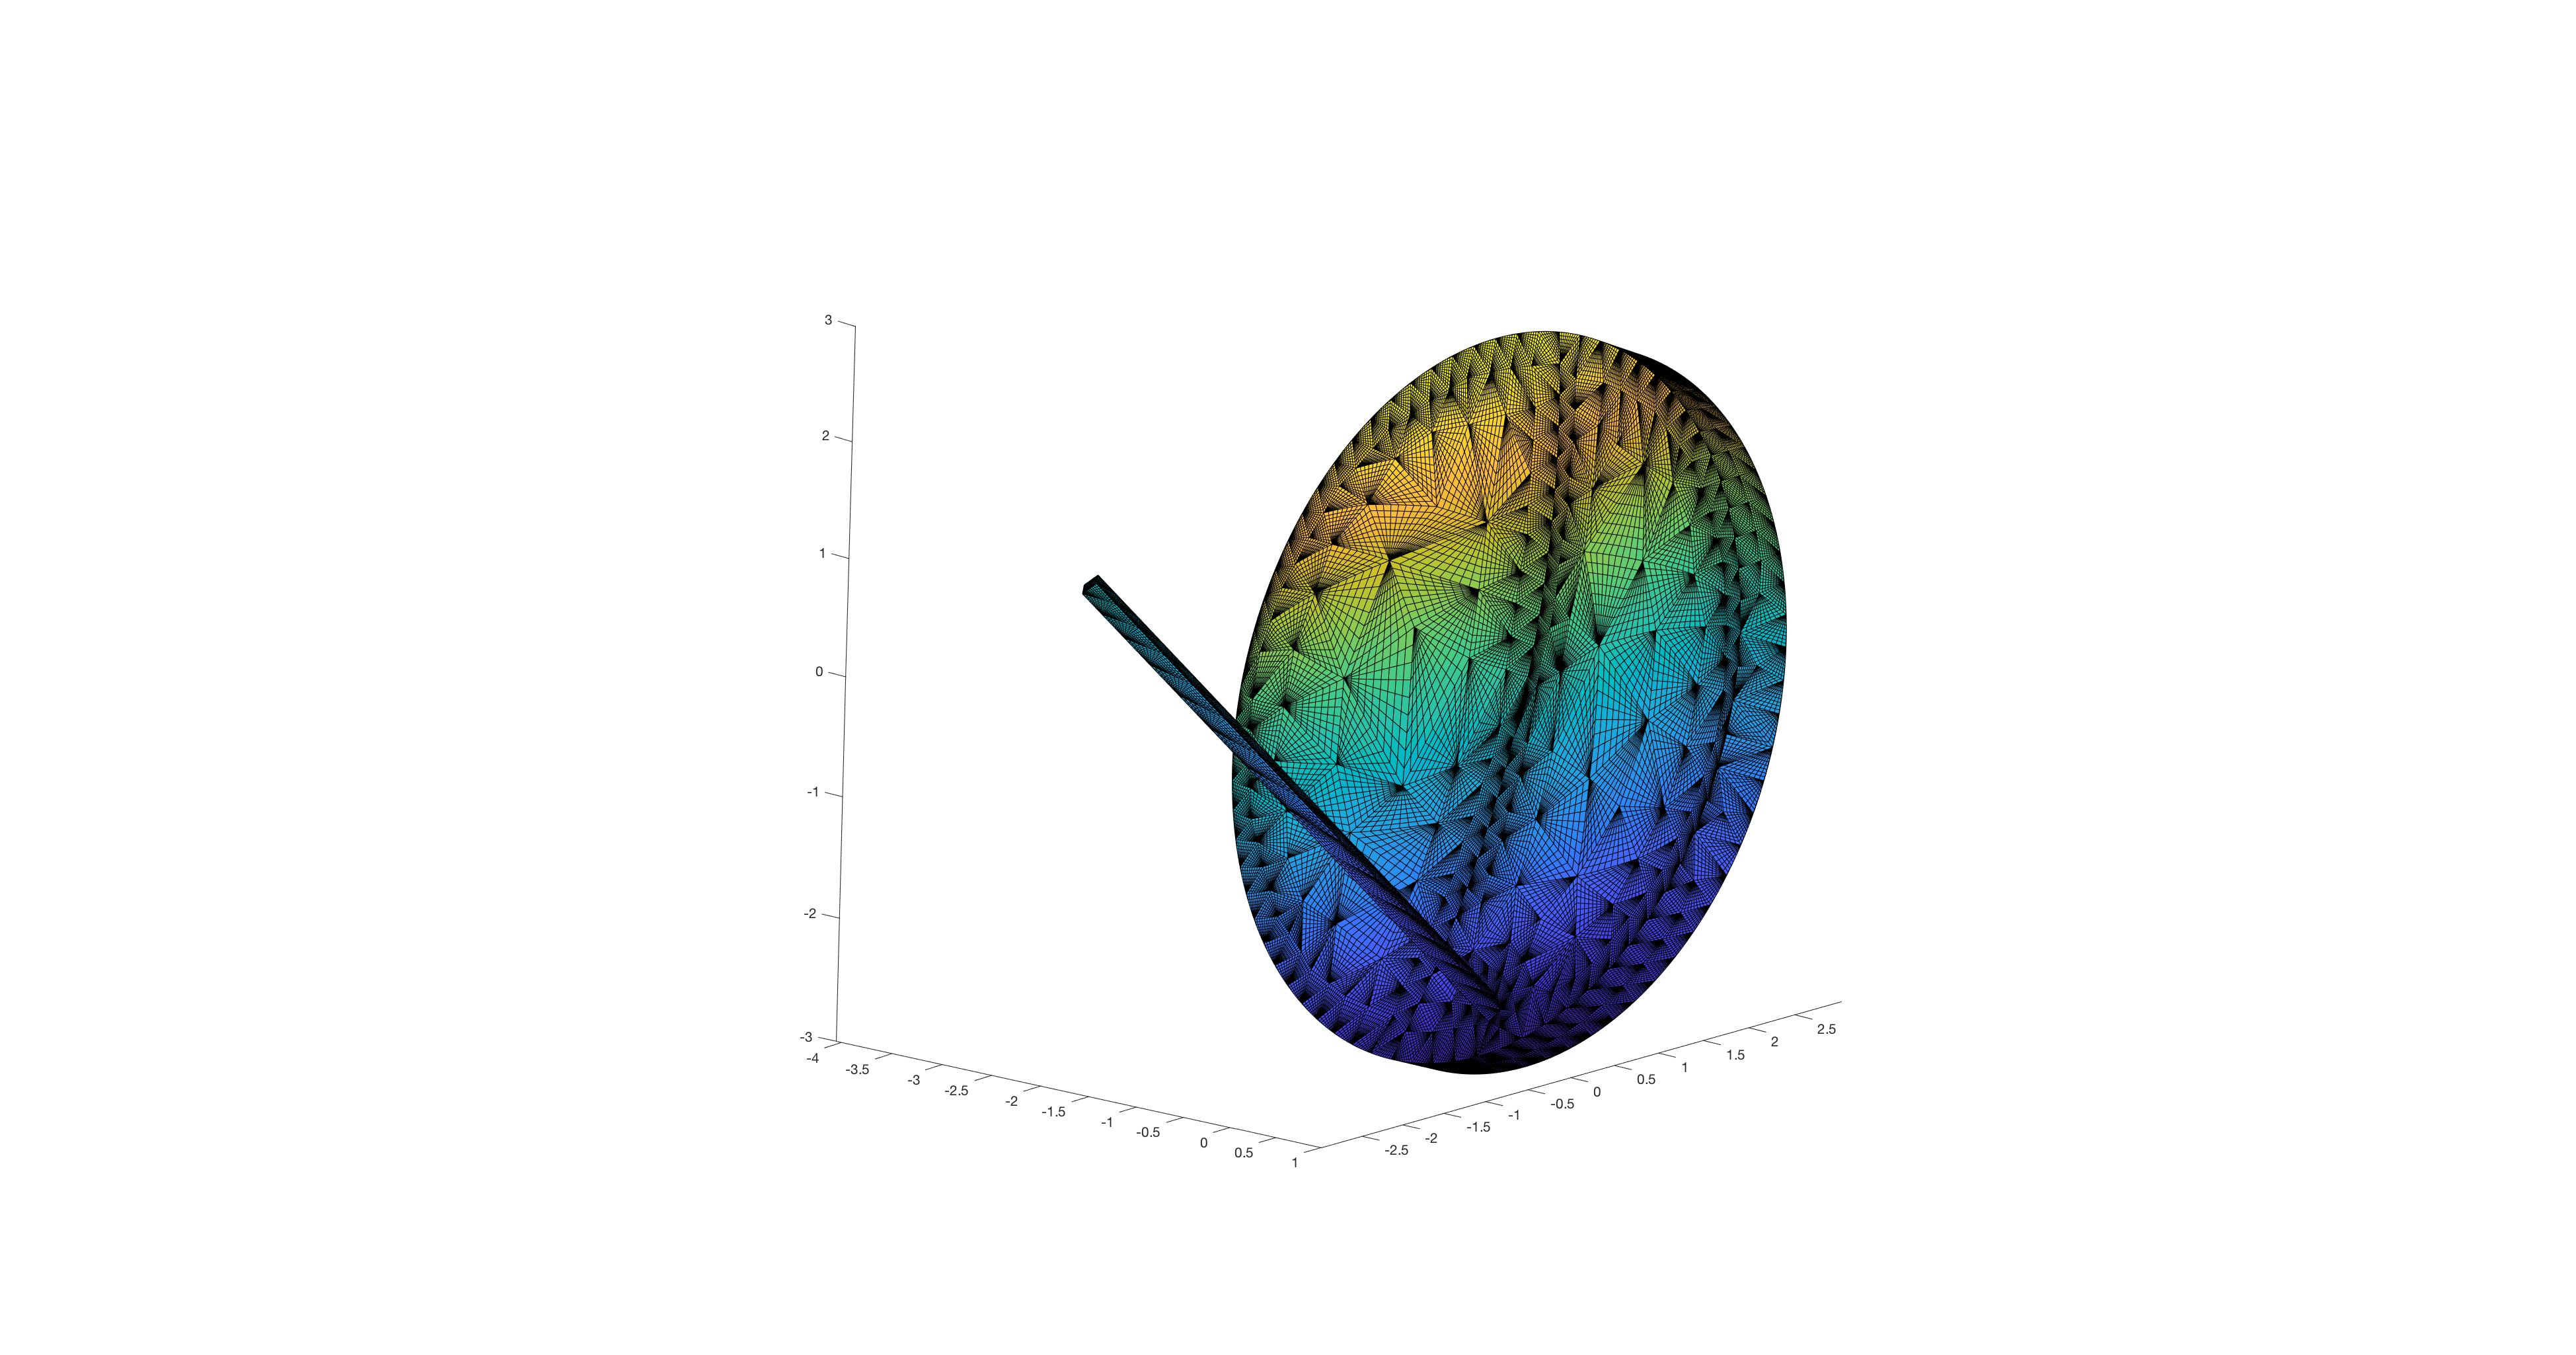
\includegraphics[width=6in]{parabolic_antenna_skeleton.pdf}
\end{center}
\caption{}
\label{parabolic_antenna_skeleton}
\end{figure}







\newpage
\subsection{two\_cavity\_filter\_1.msh (adaptive\_flag=1)}
Two cavity filter with two tuning impedances at the center of each cavity. No refinement study yet, accuracy obtained for $n_{refinement}=0$ and n\_order\_sf=45 is $Err=6\cdot 10^{-8}$


\begin{figure}[H]
\begin{center}
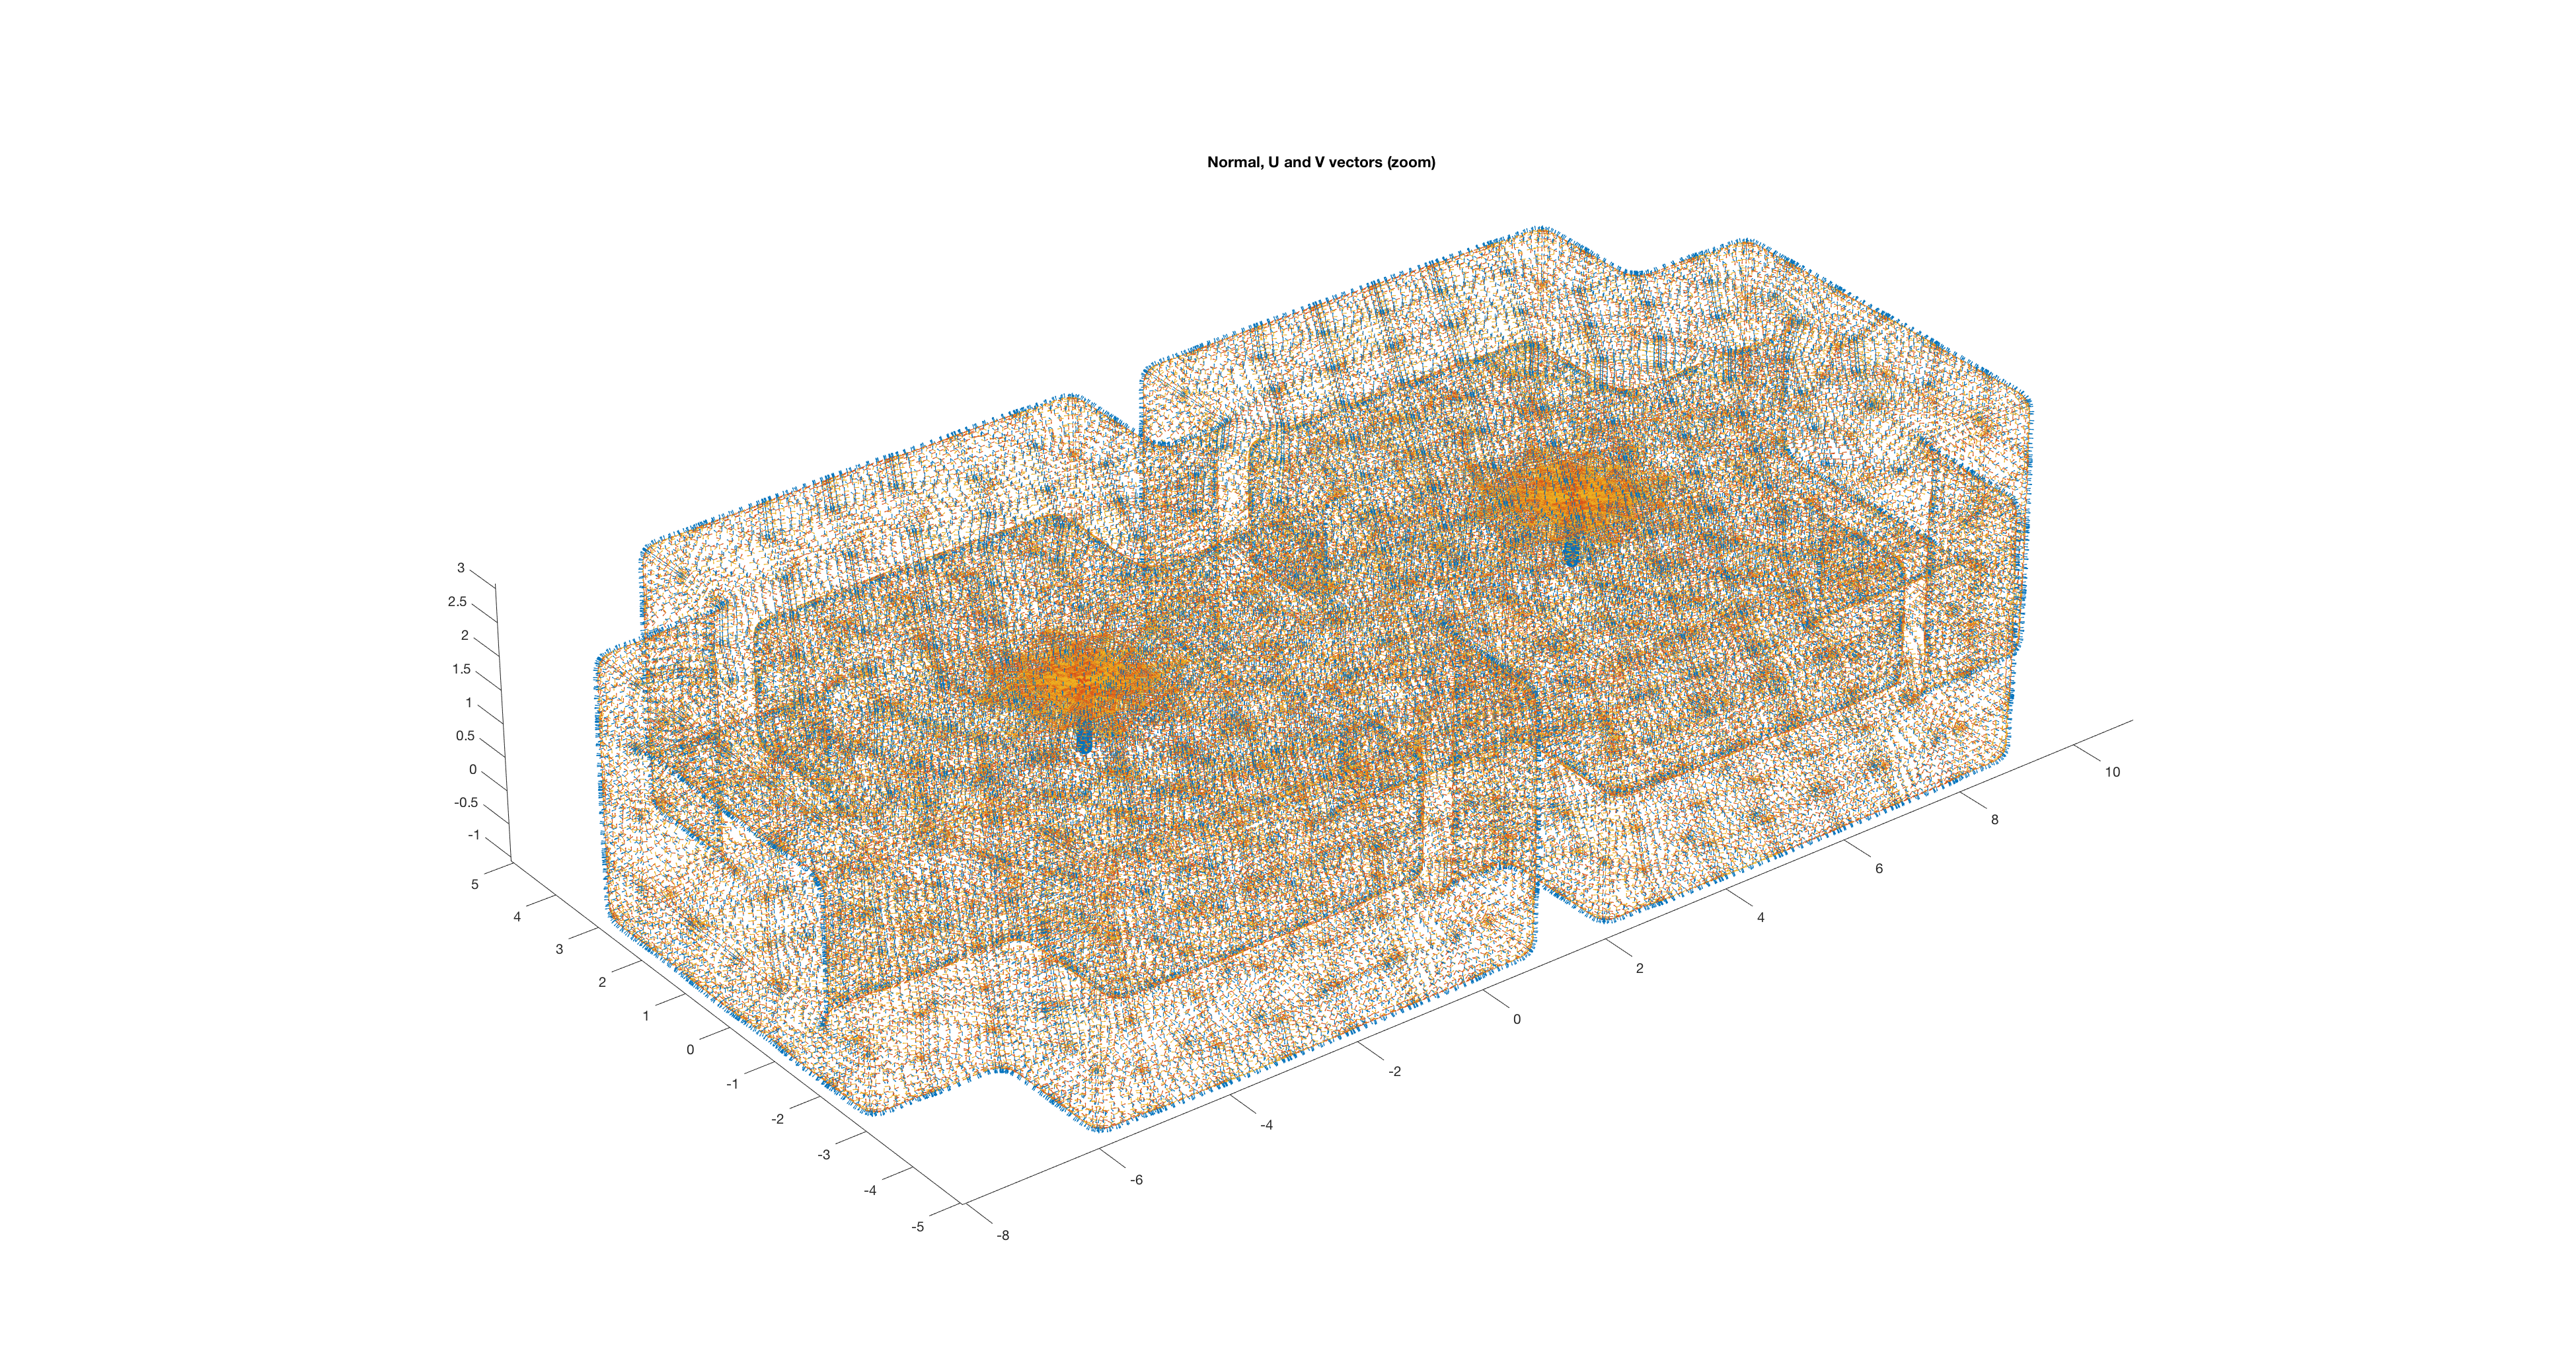
\includegraphics[width=7in]{two_cavity_filter_1.pdf}
\end{center}
\caption{}
\label{two_cavity_filter_1}
\end{figure}

\begin{figure}[H]
\begin{center}
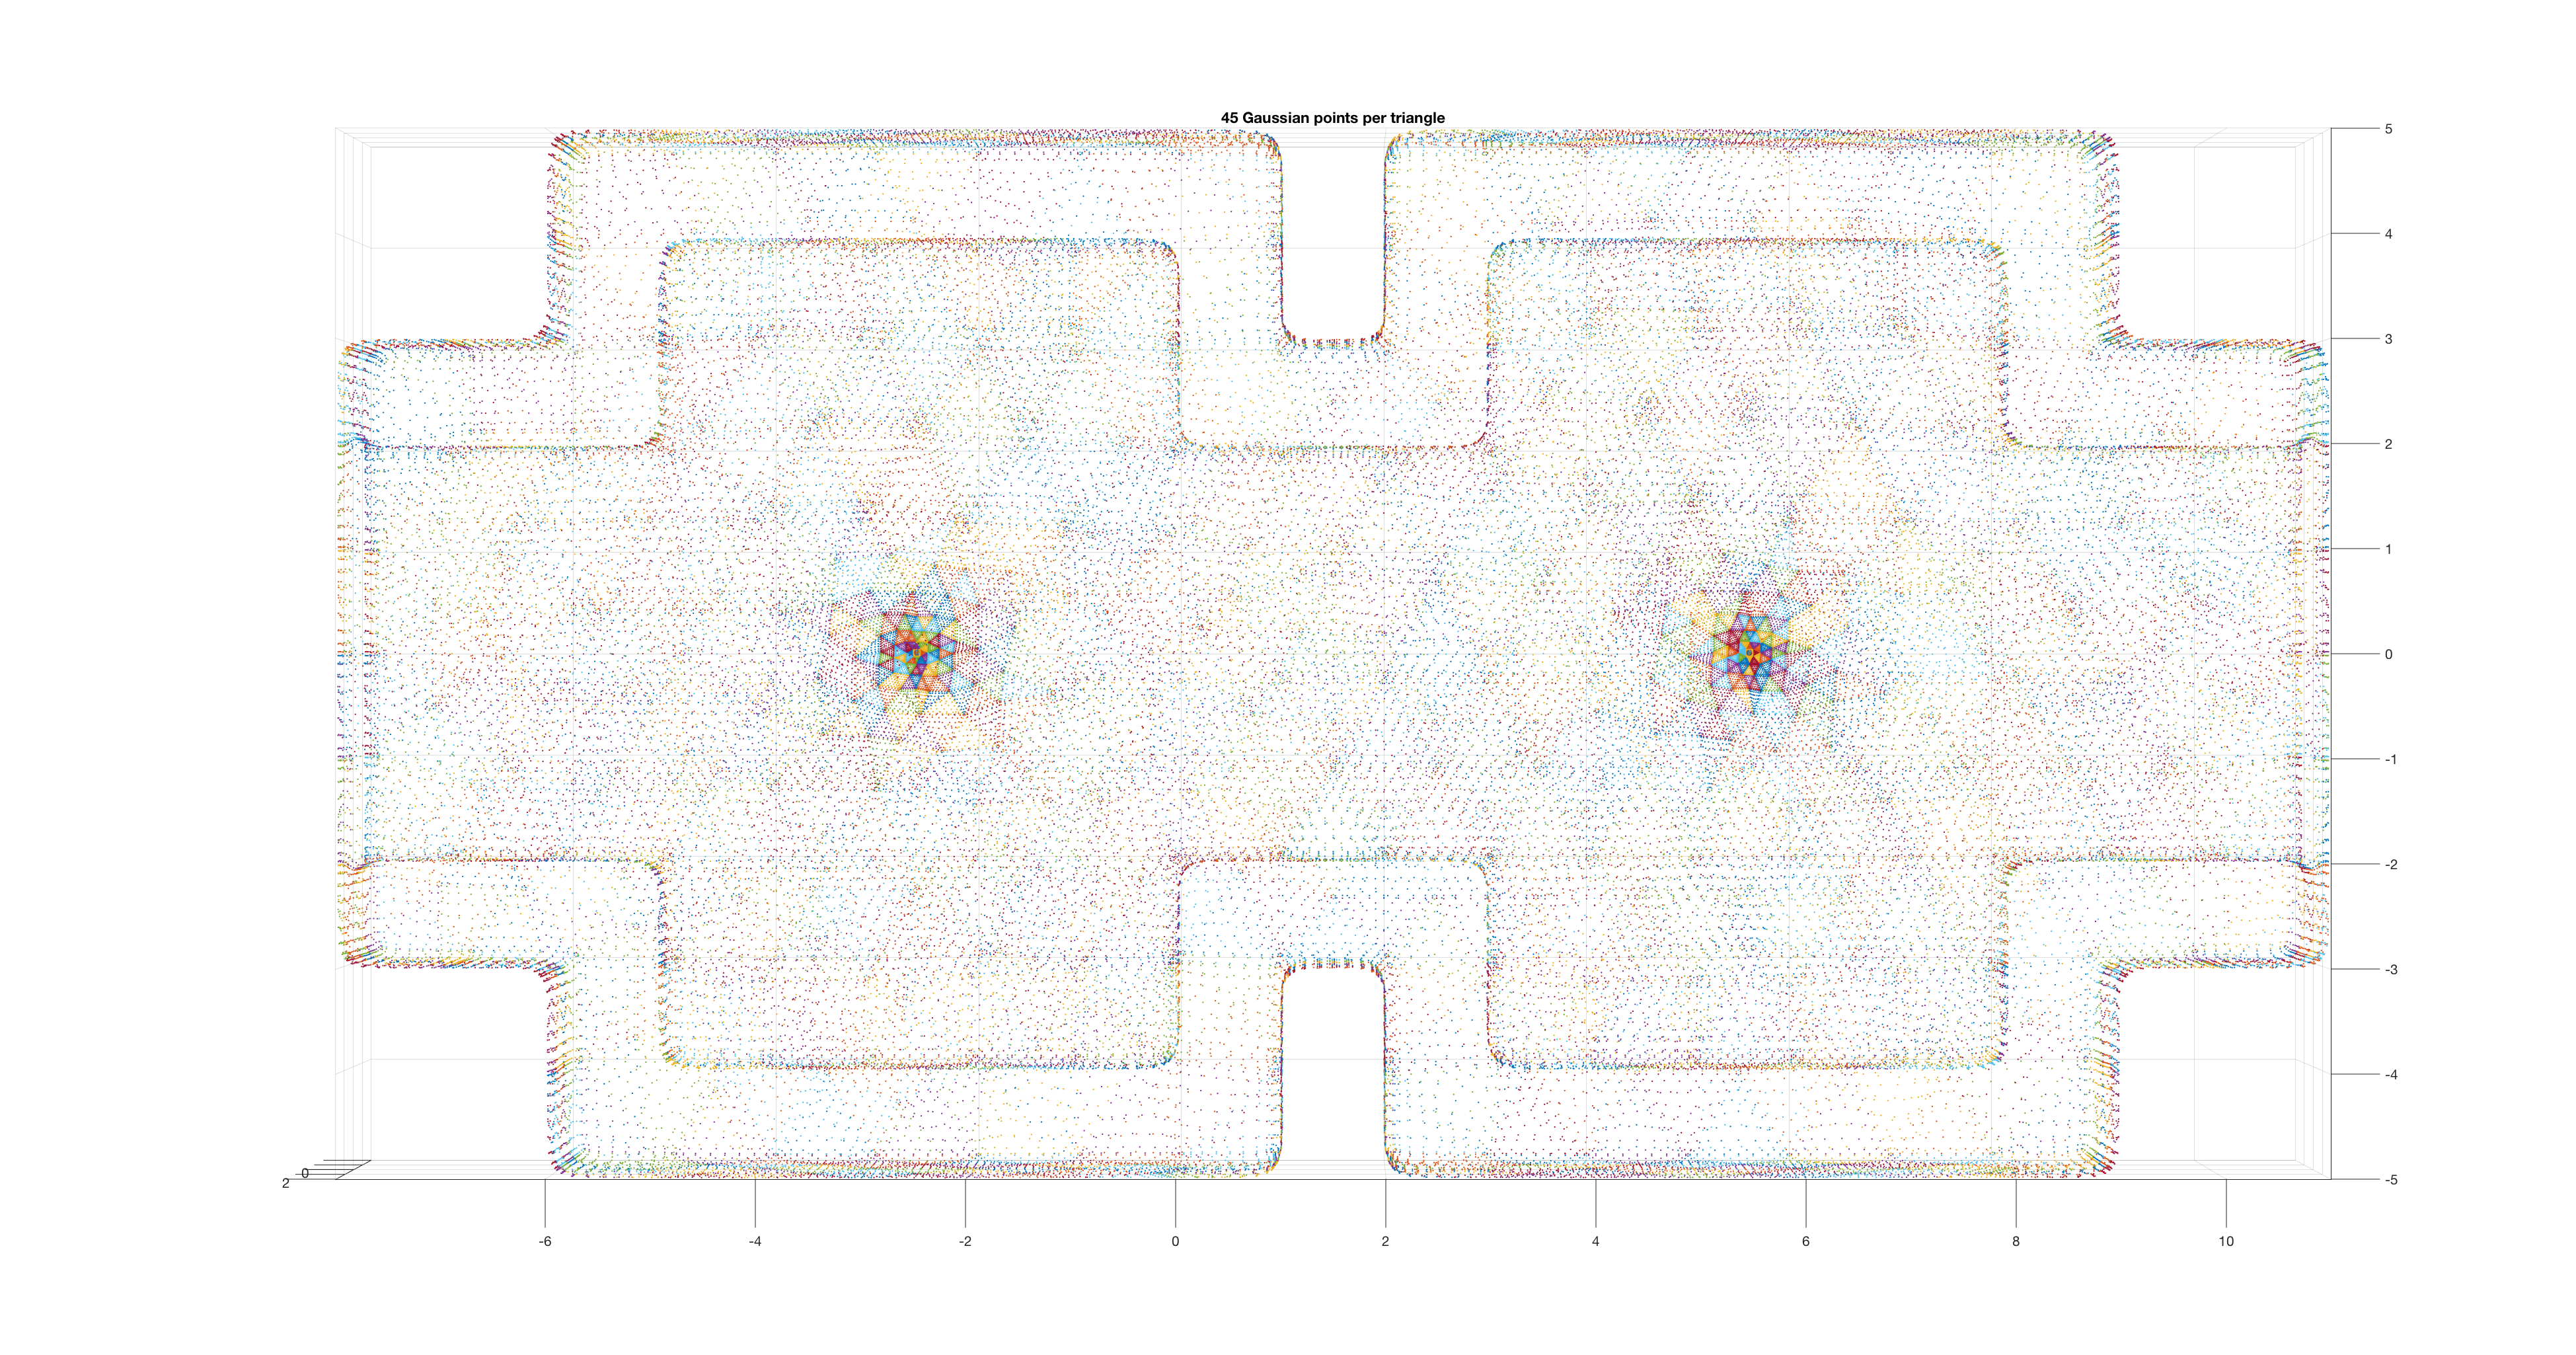
\includegraphics[width=6in]{two_cavity_filter_2.pdf}
\end{center}
\caption{}
\label{two_cavity_filter_2}
\end{figure}

\begin{figure}[H]
\begin{center}
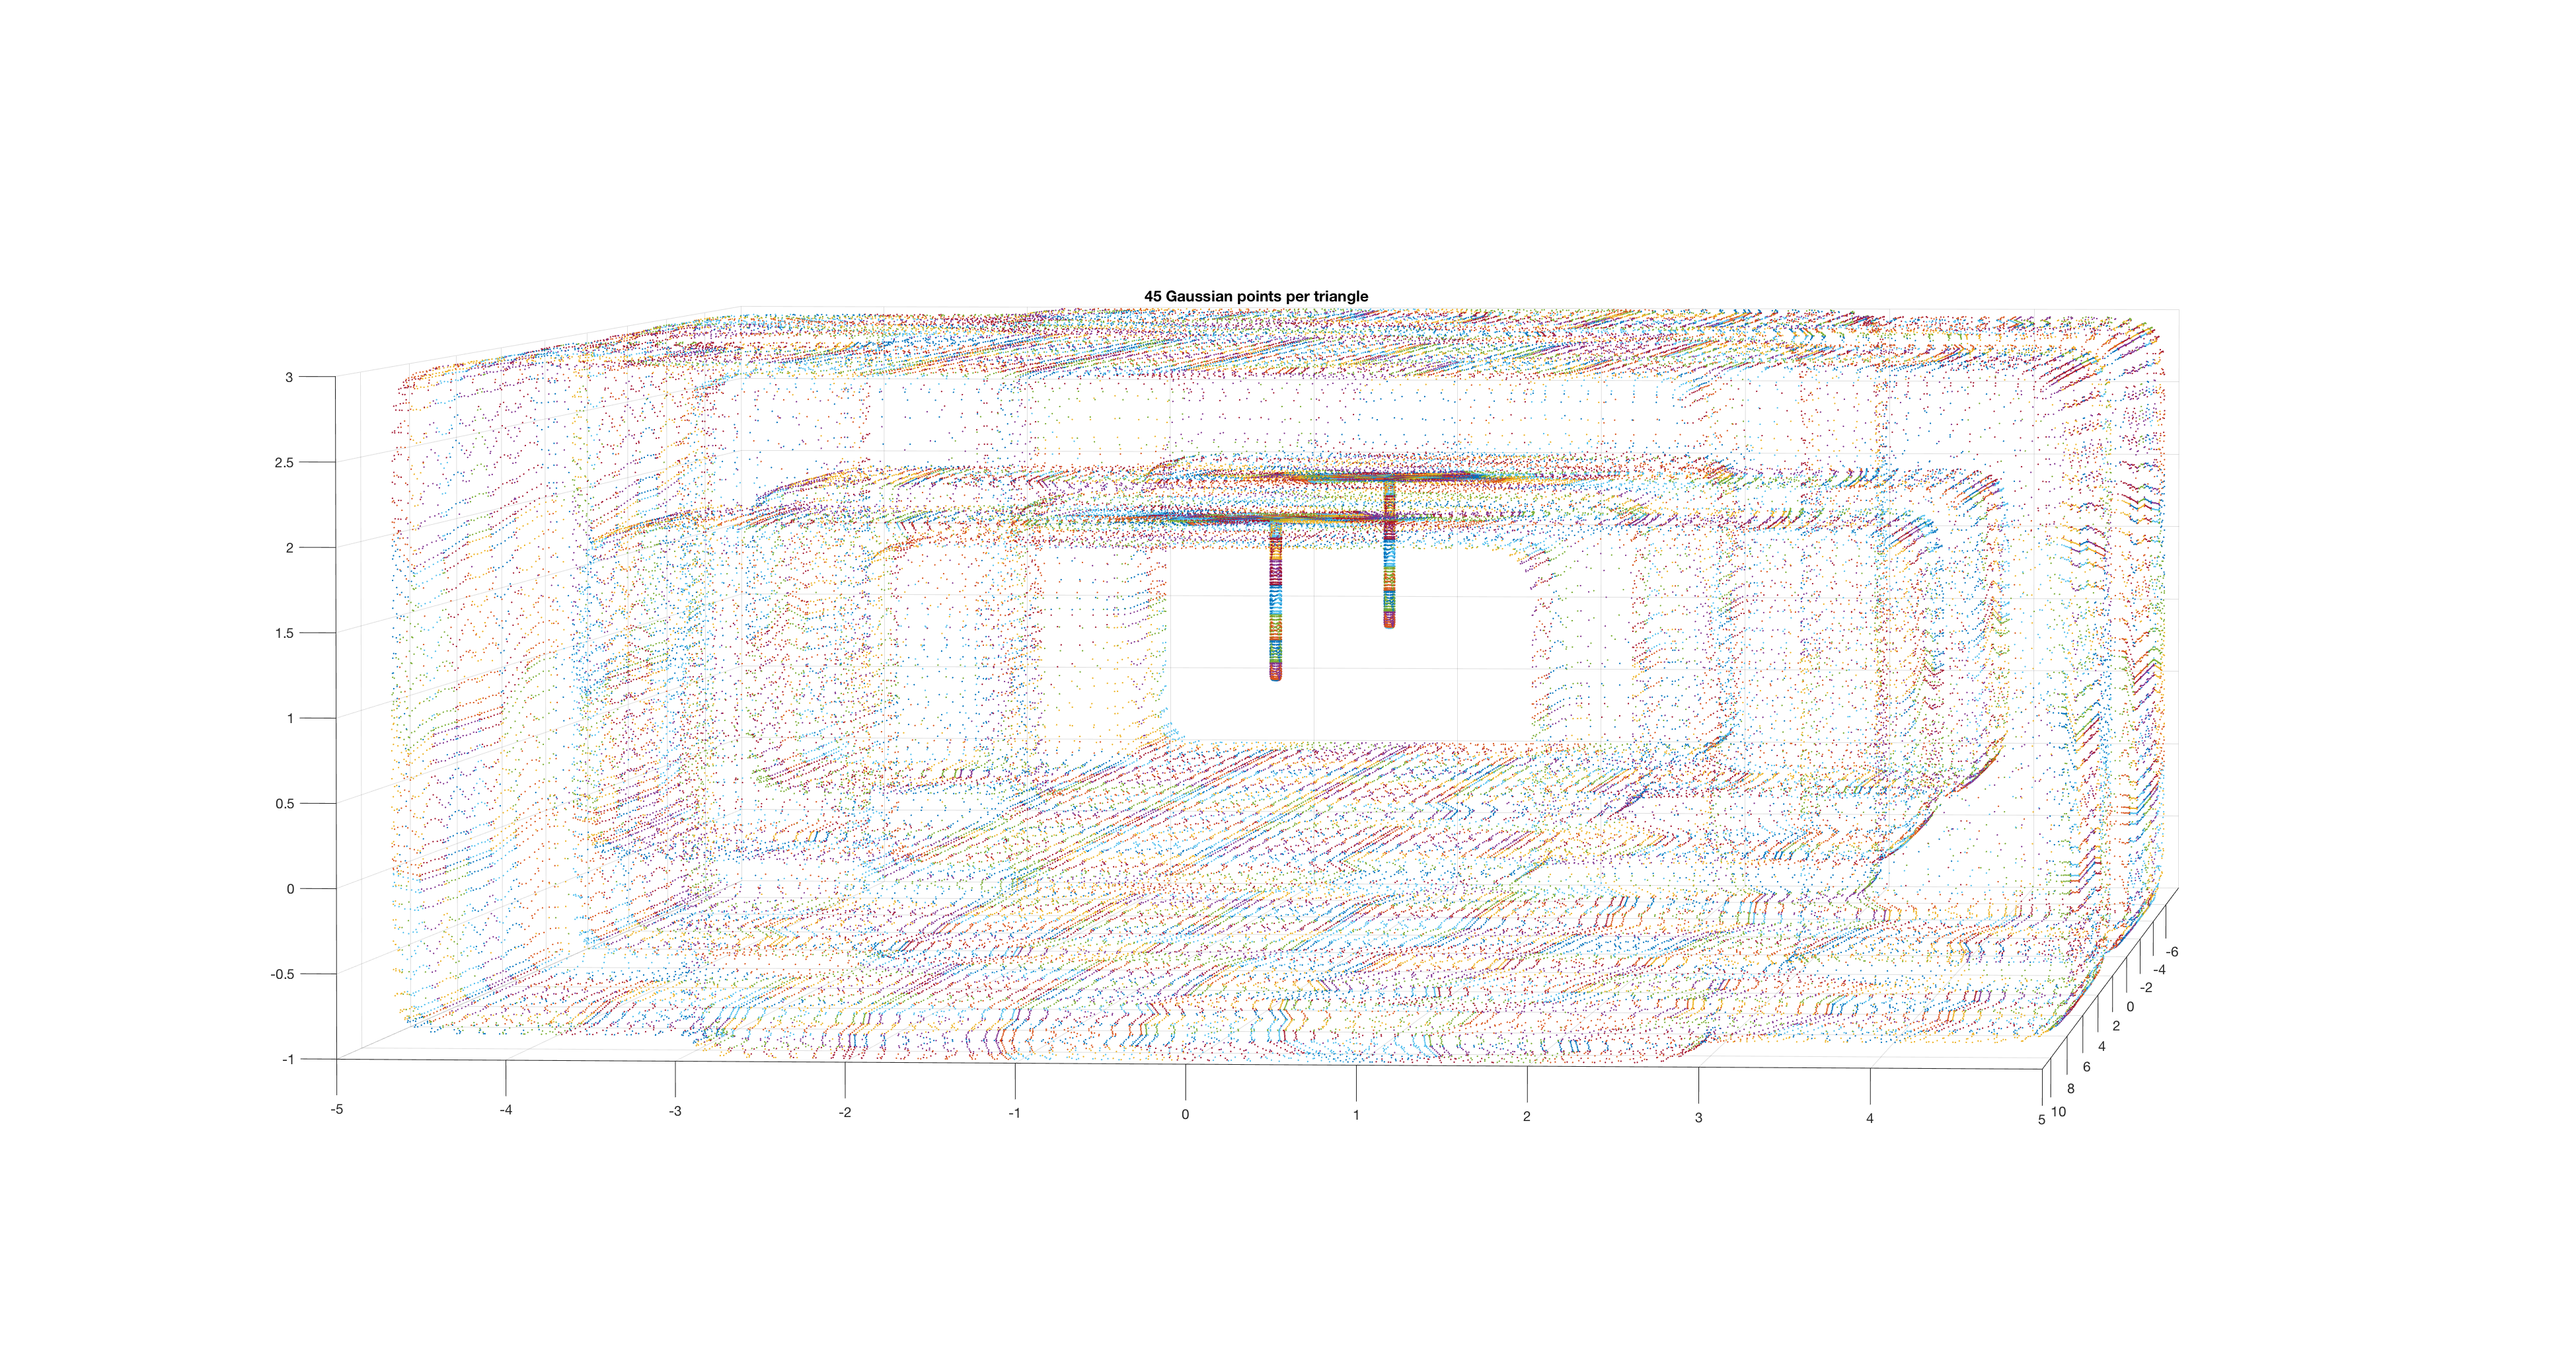
\includegraphics[width=6in]{two_cavity_filter_3.pdf}
\end{center}
\caption{}
\label{two_cavity_filter_3}
\end{figure}



\begin{figure}[H]
\begin{center}
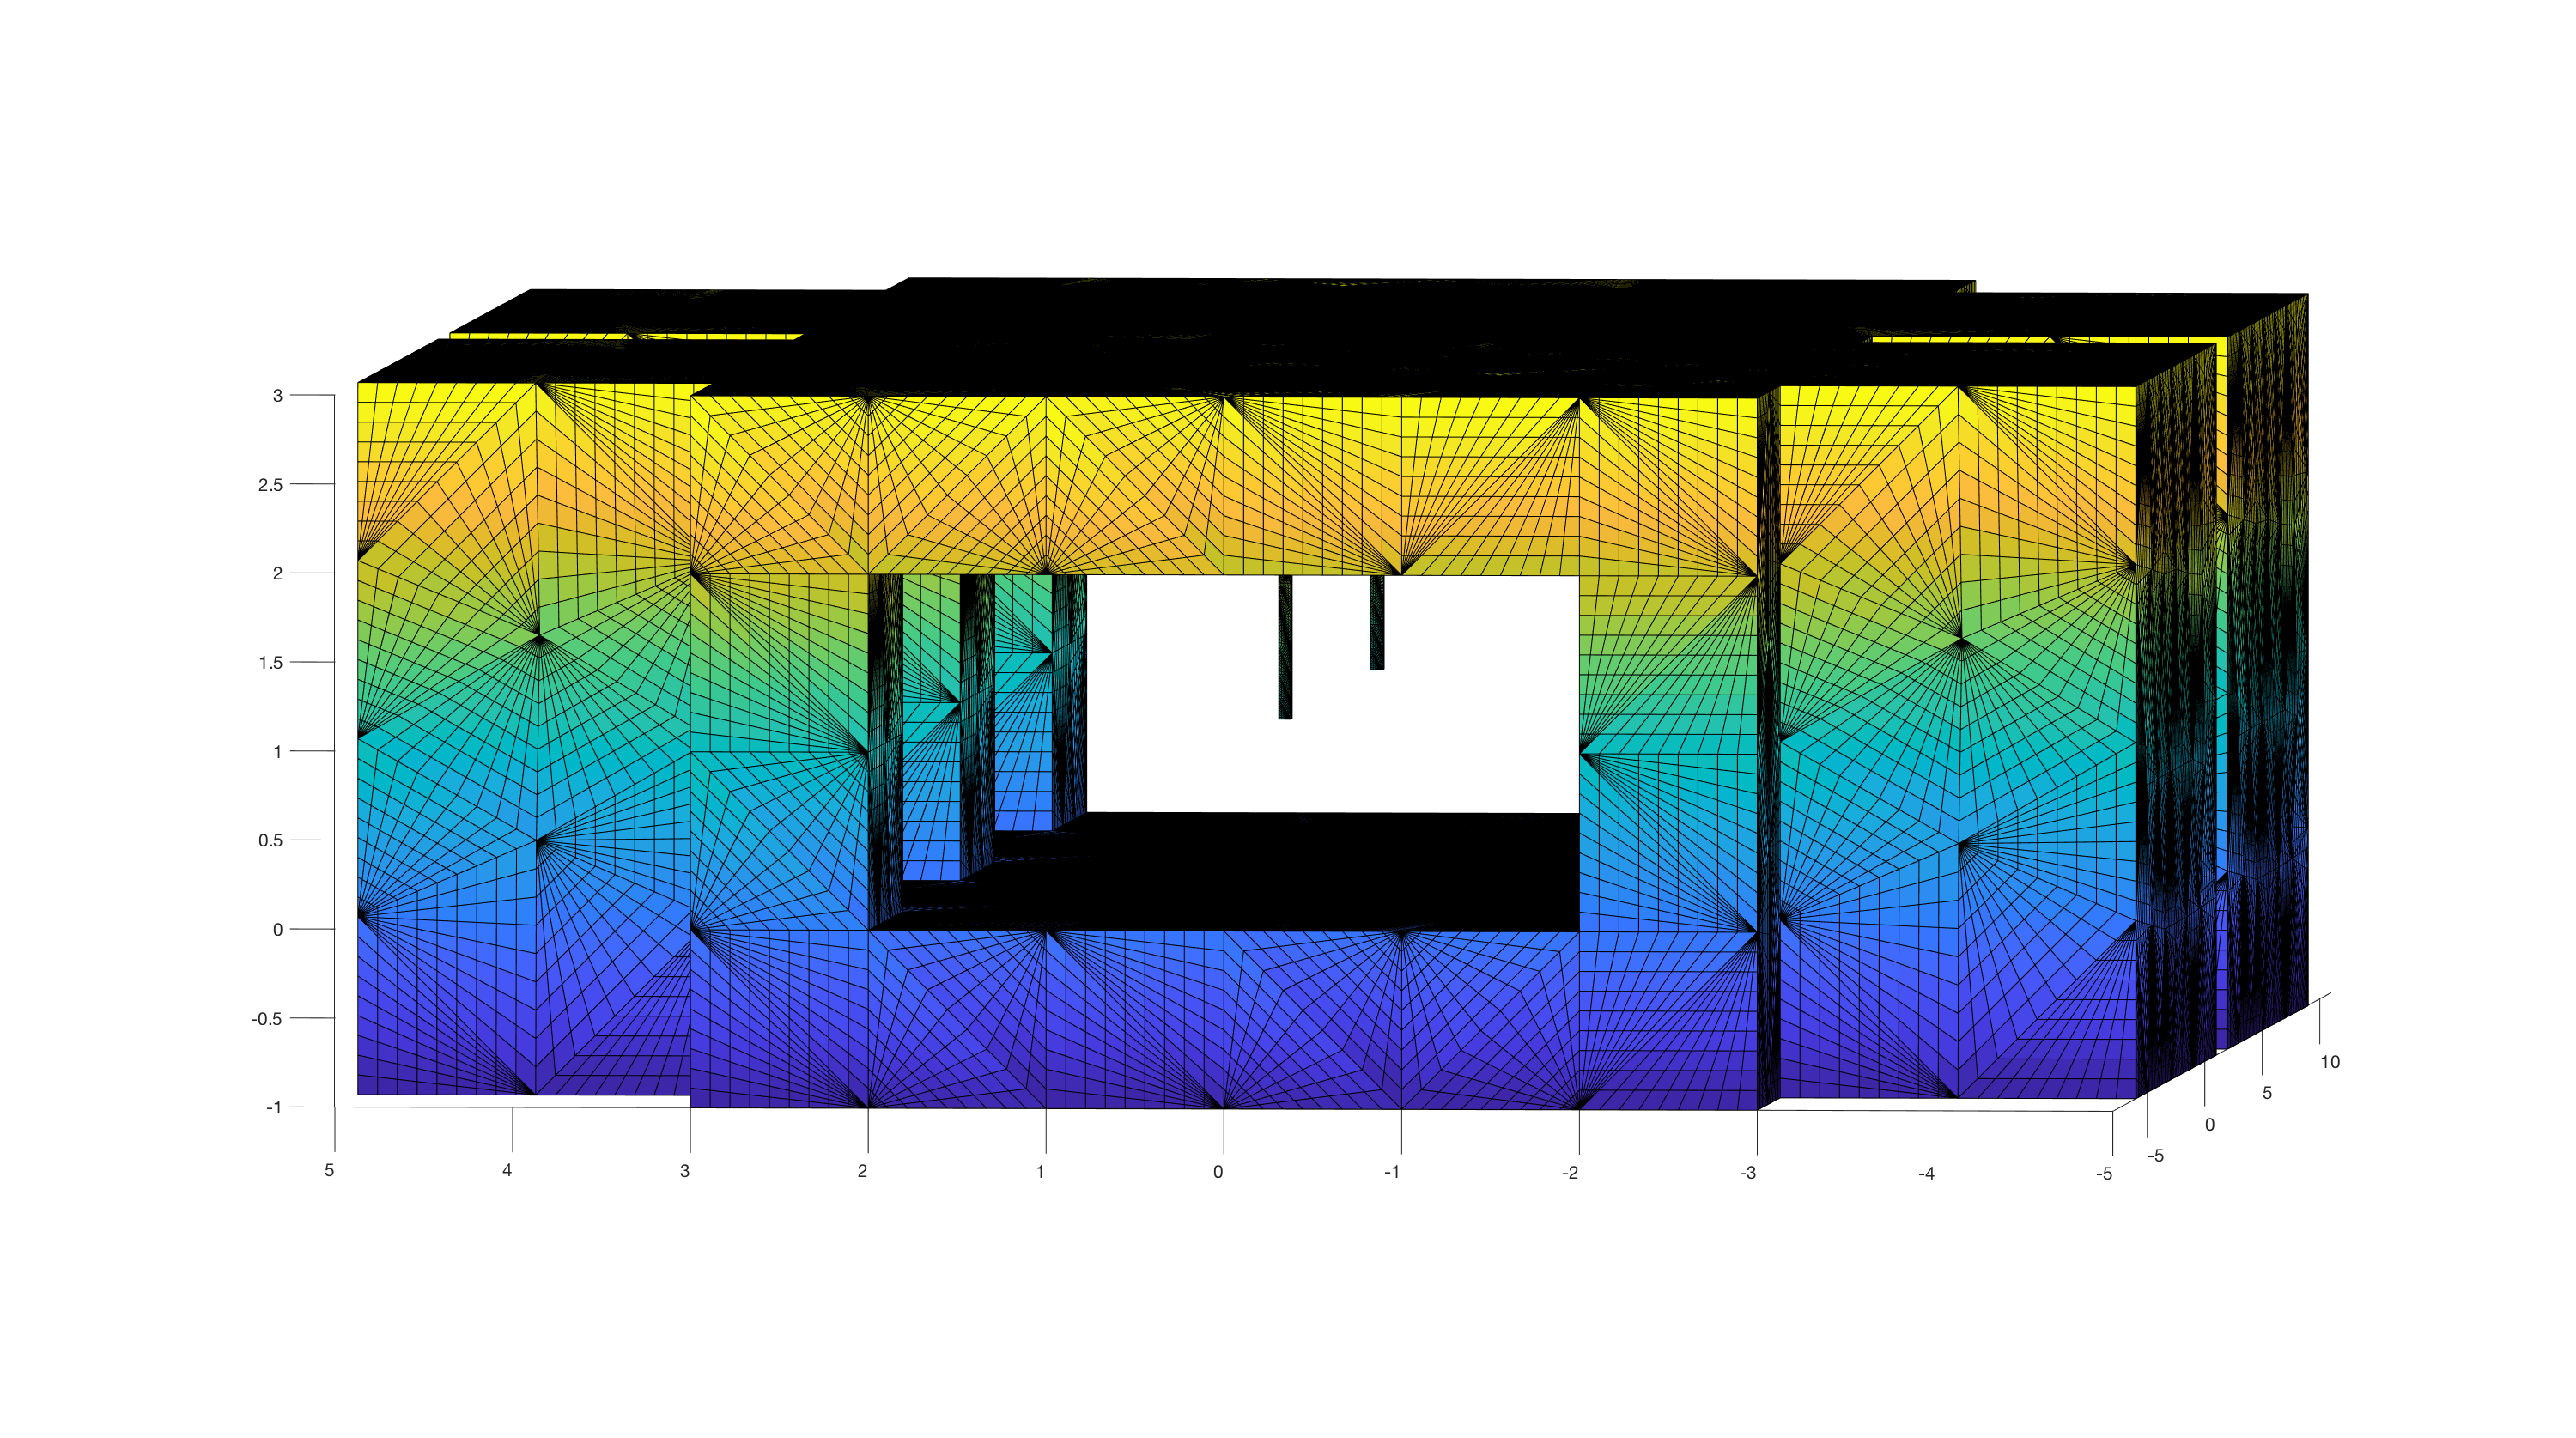
\includegraphics[width=6in]{two_cavity_filter_skeleton.pdf}
\end{center}
\caption{View of the skeleton. Detail of the tuning impedances}
\label{two_cavity_filter_skeleton}
\end{figure}


\begin{figure}[H]
\begin{center}
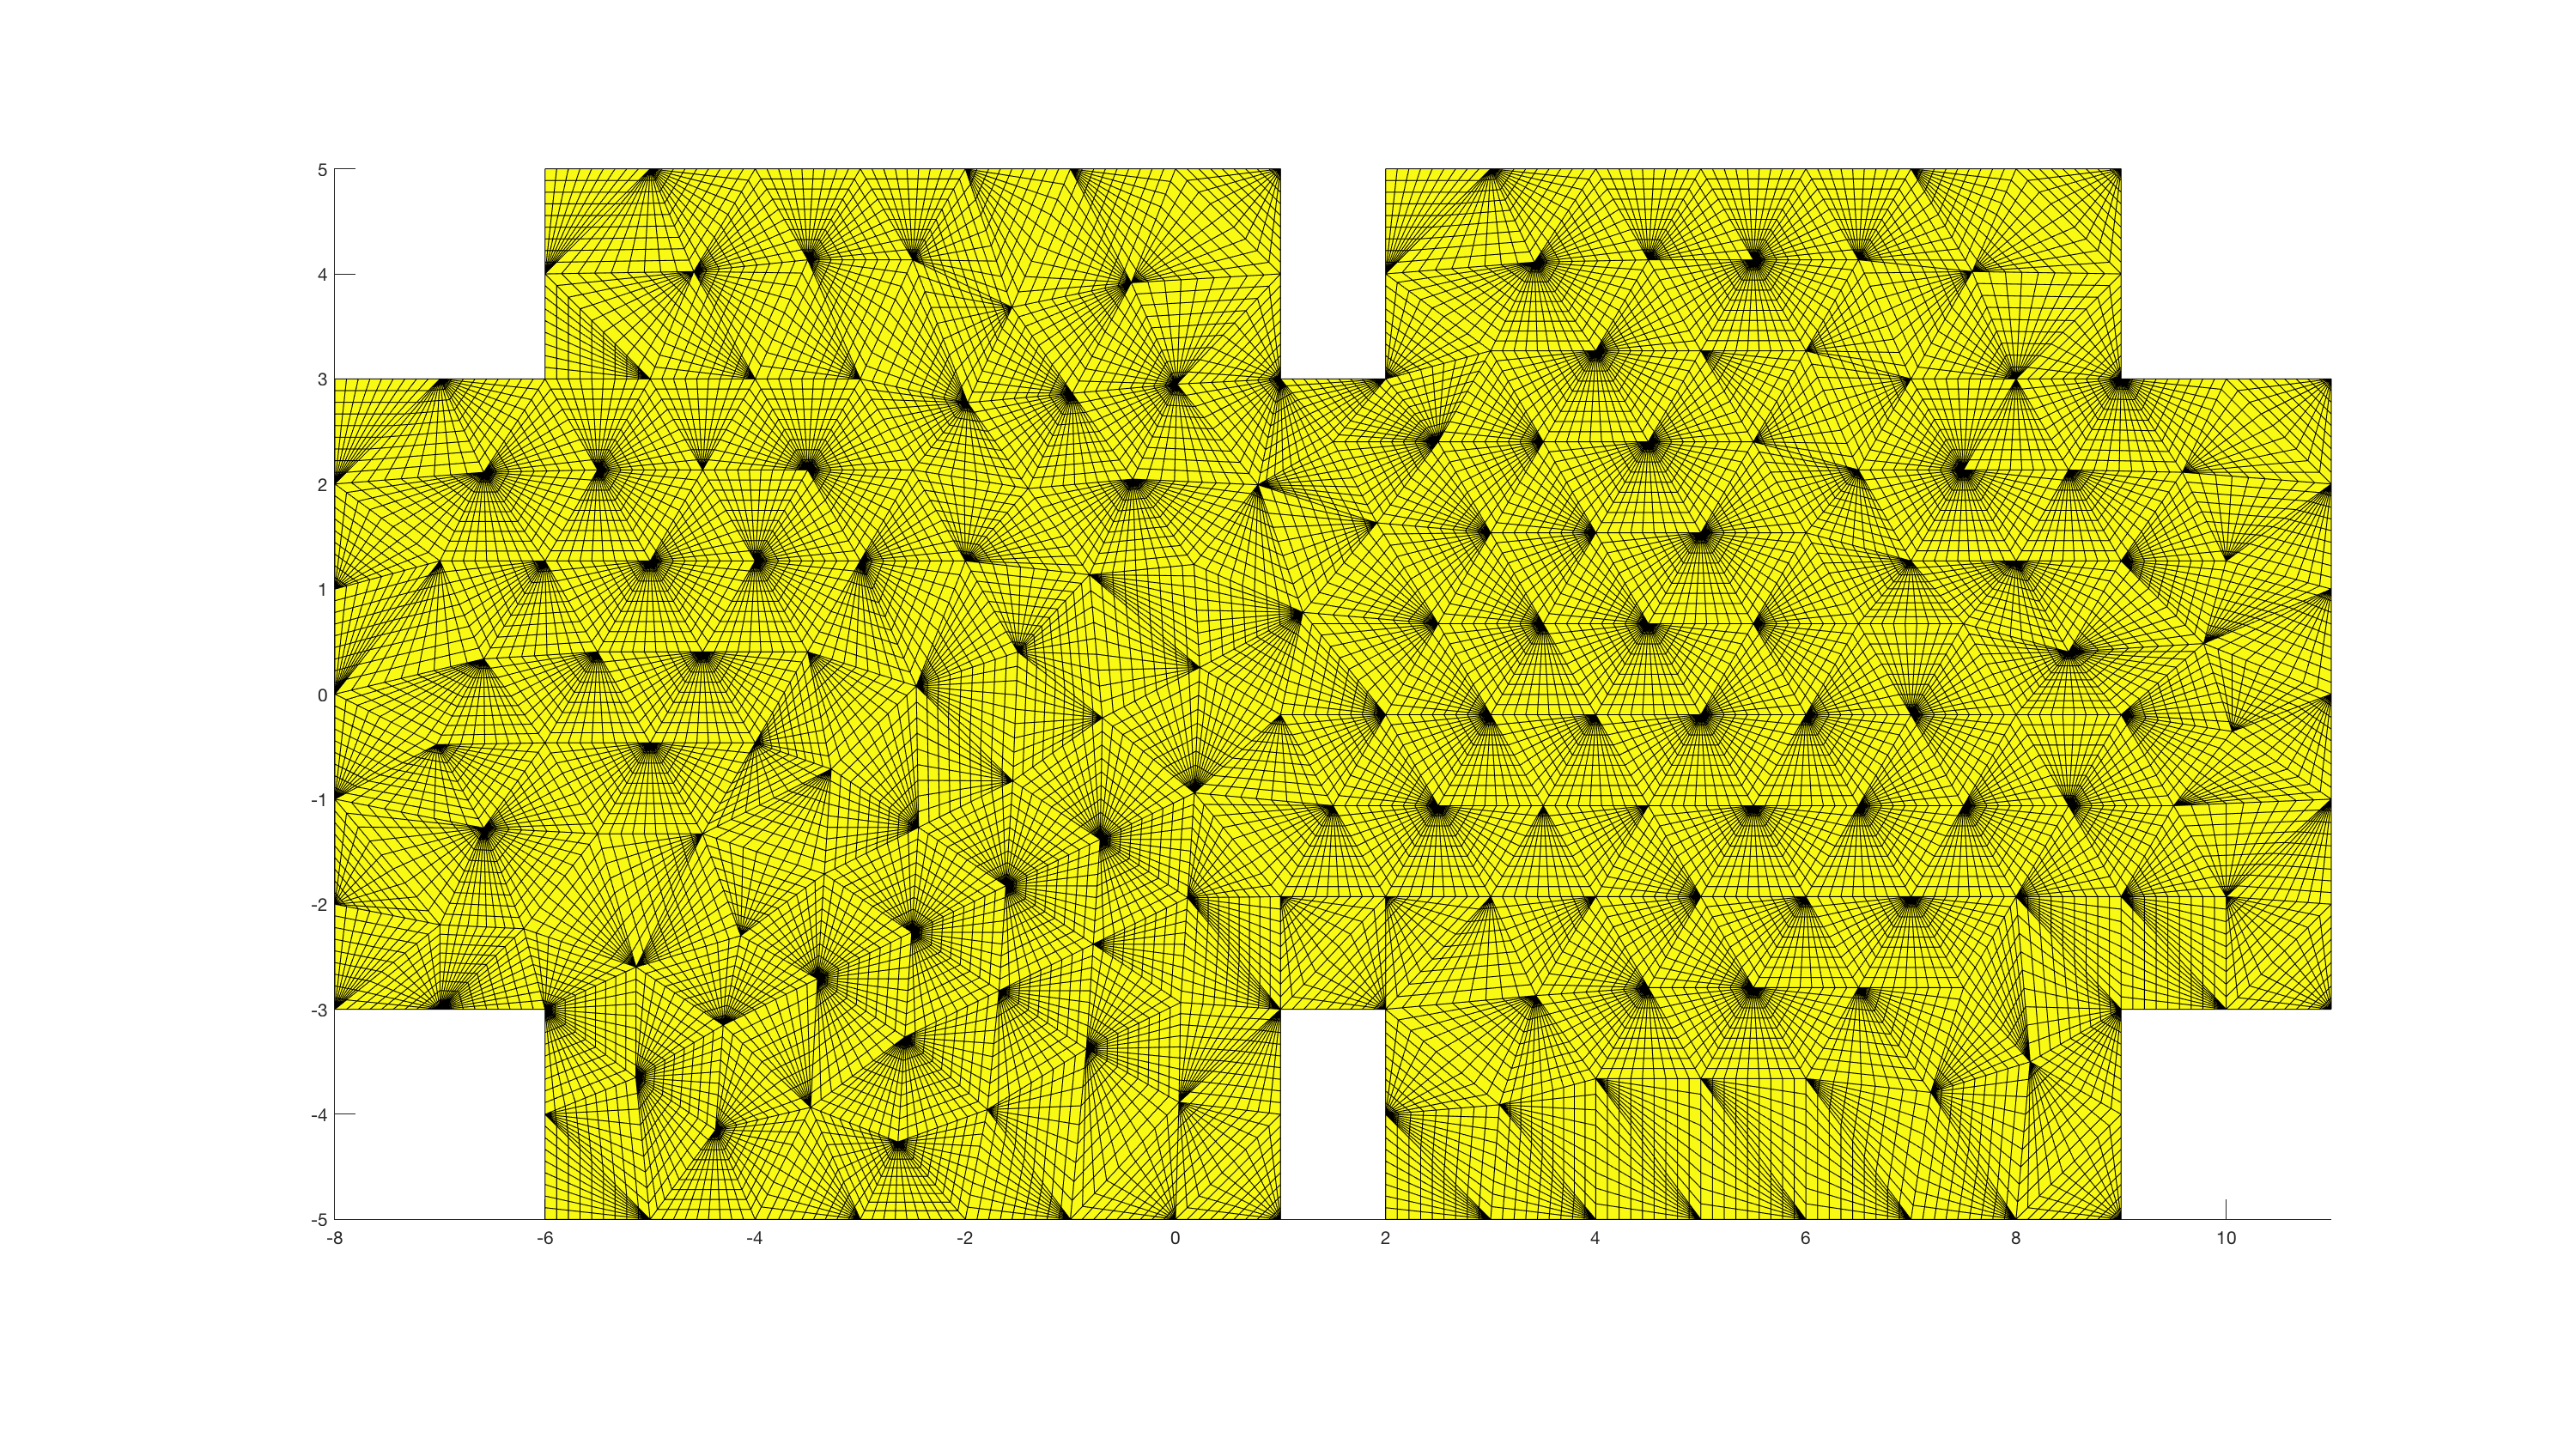
\includegraphics[width=6in]{two_cavity_filter_skeleton_2.pdf}
\end{center}
\caption{Top view of the skeleton}
\label{two_cavity_filter_skeleton}
\end{figure}


\newpage

\subsection{mi\_barco\_simple\_13.msh (adaptive\_flag=1)}
Complex geometry with some small details (monopole antennas and parabolic reflector). No refinement study yet, accuracy obtained for $n_{refinement}=0$ and n\_order\_sf=45 is $Err=2.58\cdot 10^{-7}$. I tried some refinement but no acuuracy was gained. I have to study in detail which part of the ship is causing troubles. I'll study the convergence with earlier versions of the ship with fewer details. Geometries with this degree of complexity are still challenging (with this version of the code).



\begin{figure}[H]
\begin{center}
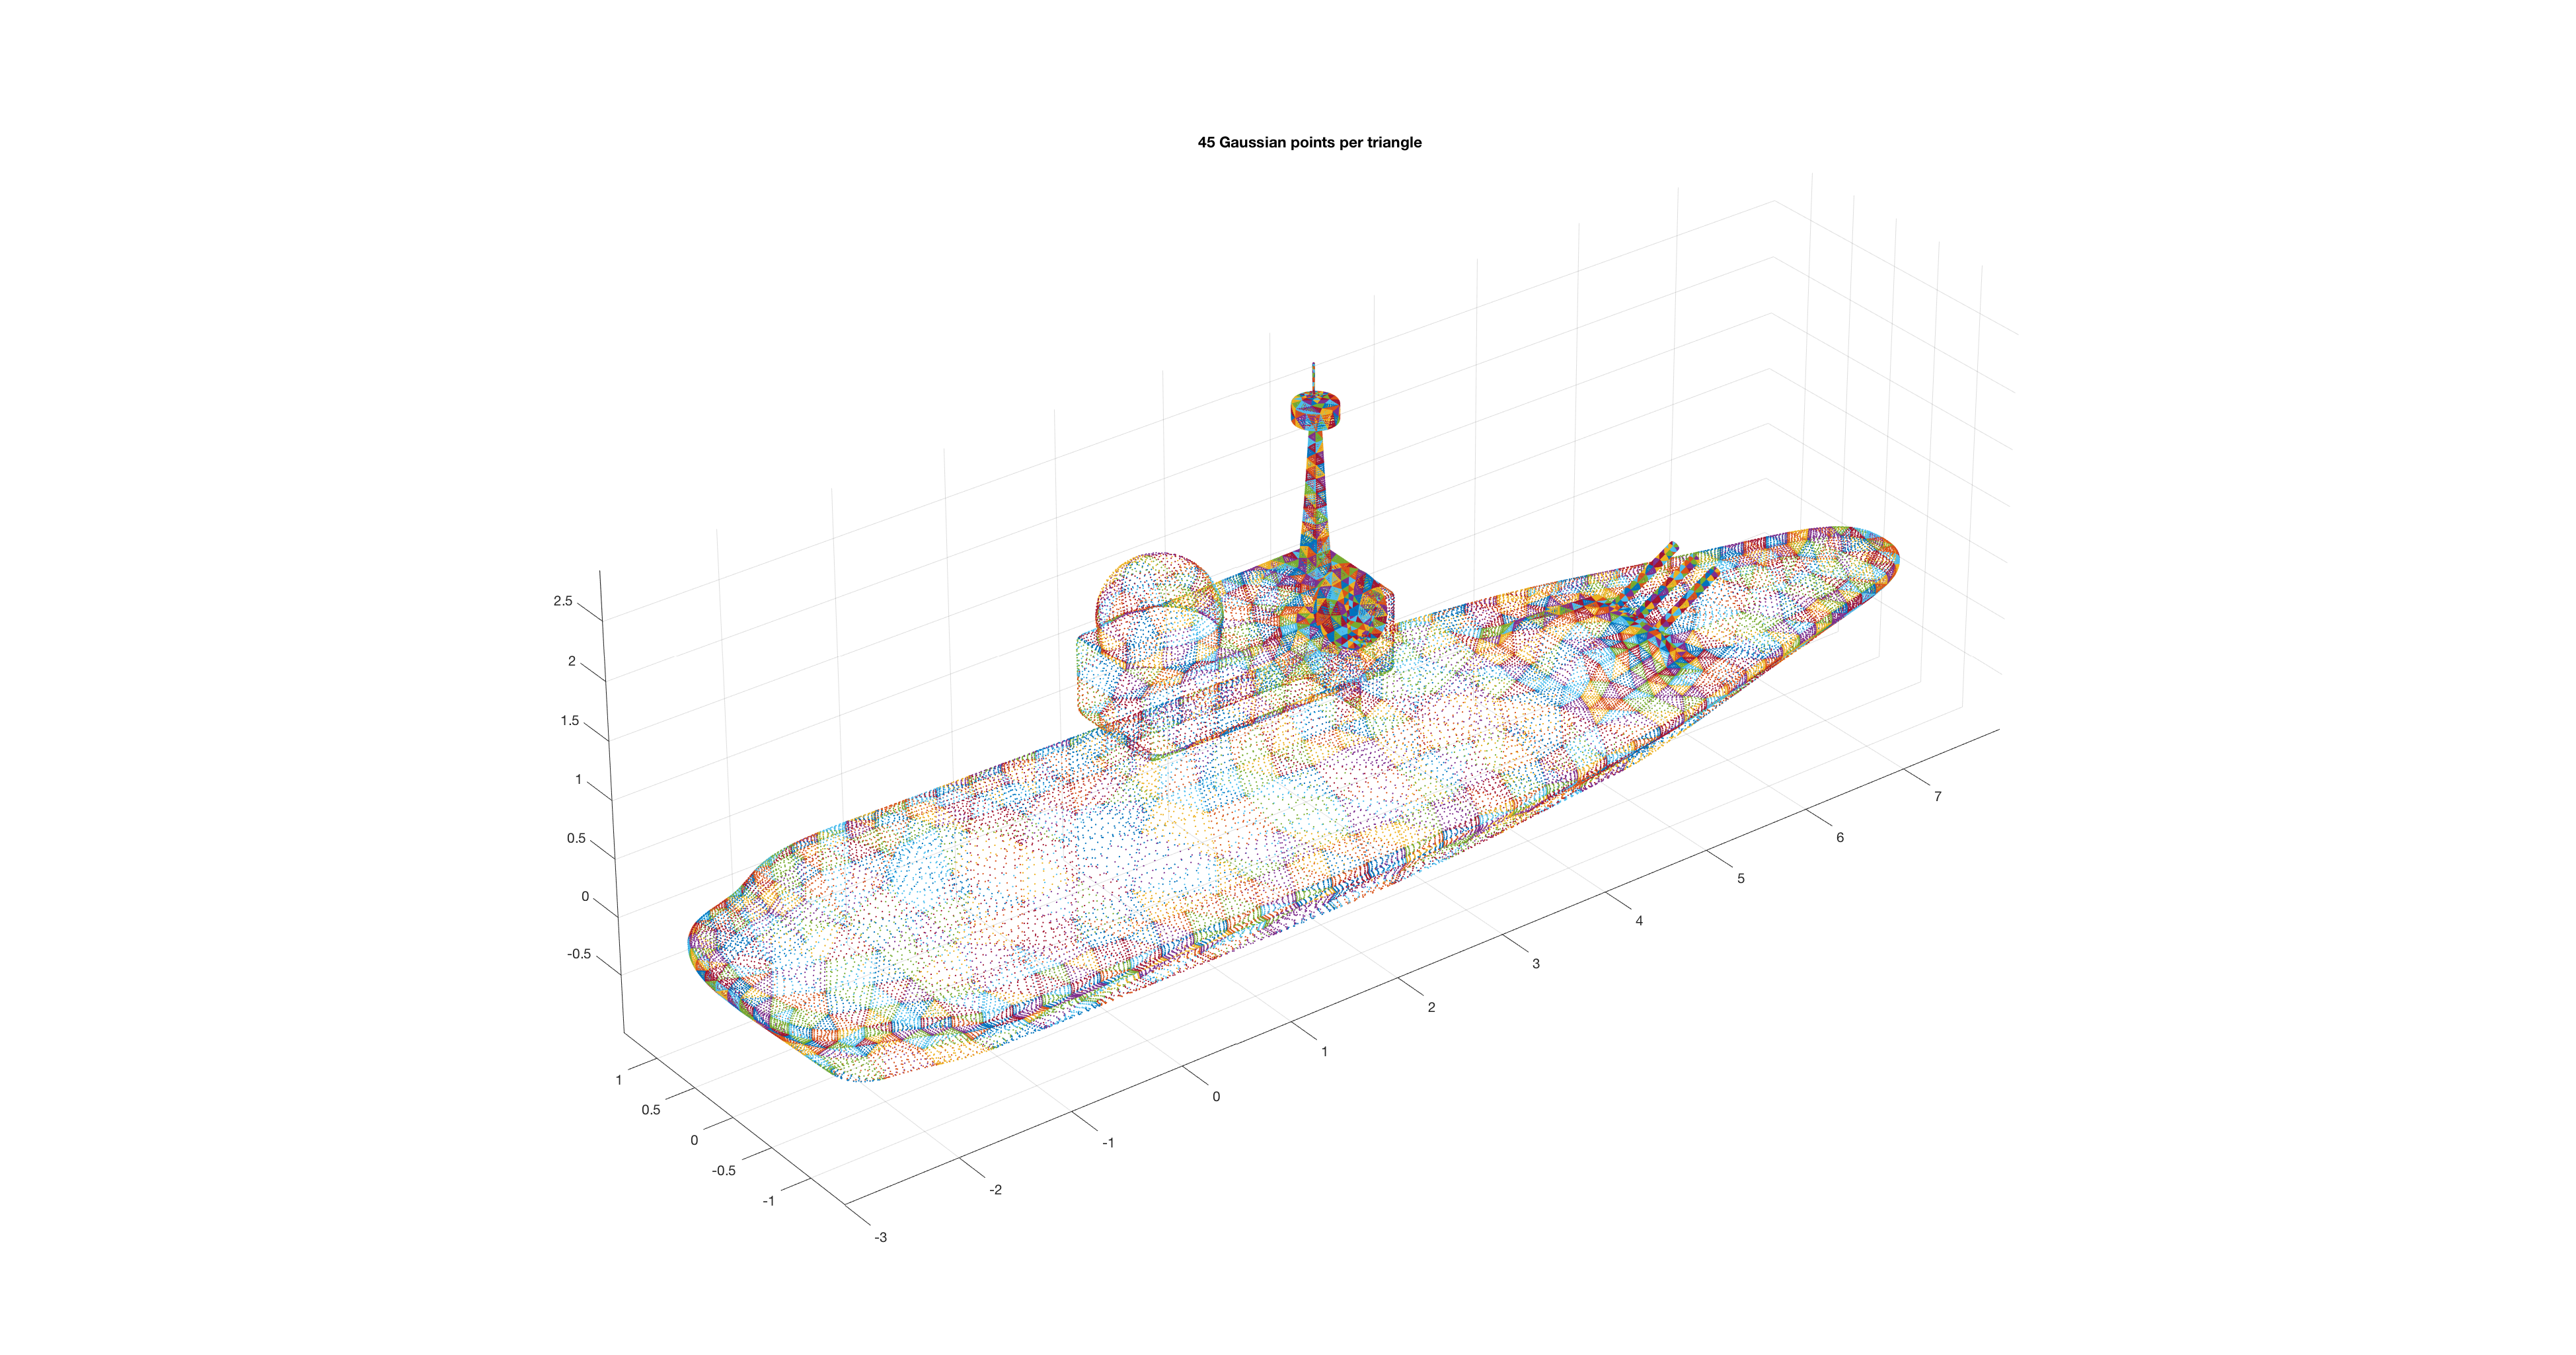
\includegraphics[width=7in]{war_ship_1.pdf}
\end{center}
\caption{}
\label{war_ship_1}
\end{figure}



\begin{figure}[H]
\begin{center}
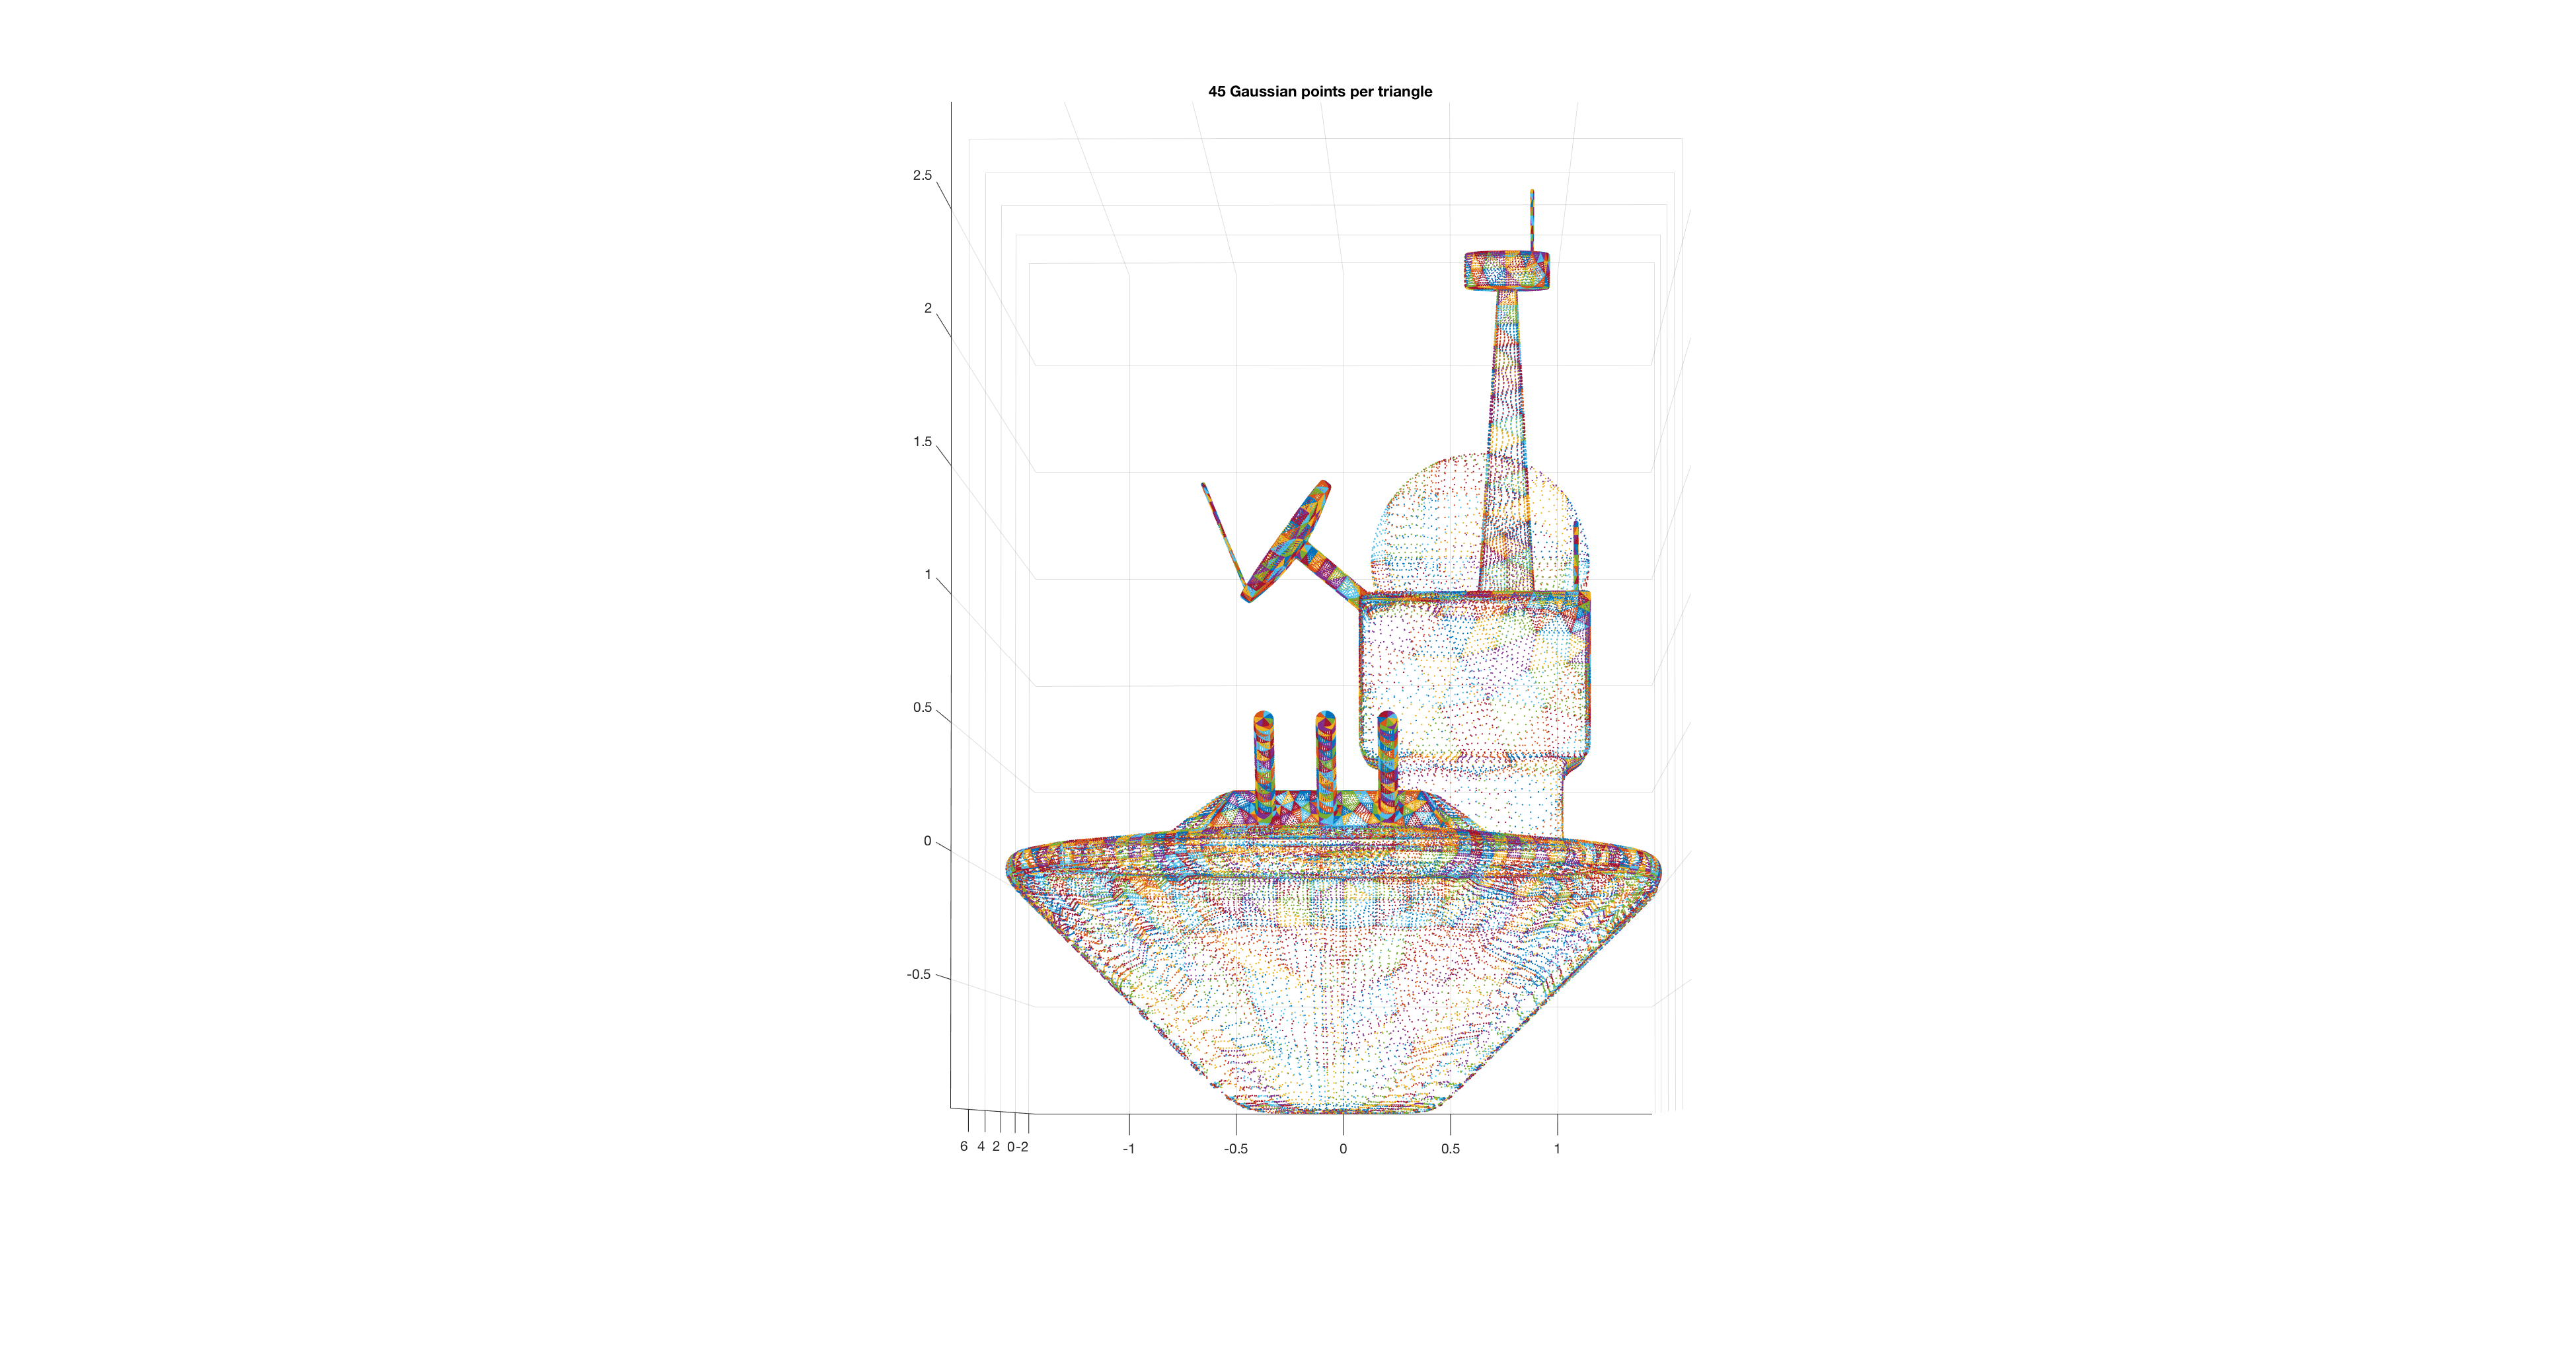
\includegraphics[width=6in]{war_ship_2.pdf}
\end{center}
\caption{}
\label{war_ship_2}
\end{figure}


\begin{figure}[H]
\begin{center}
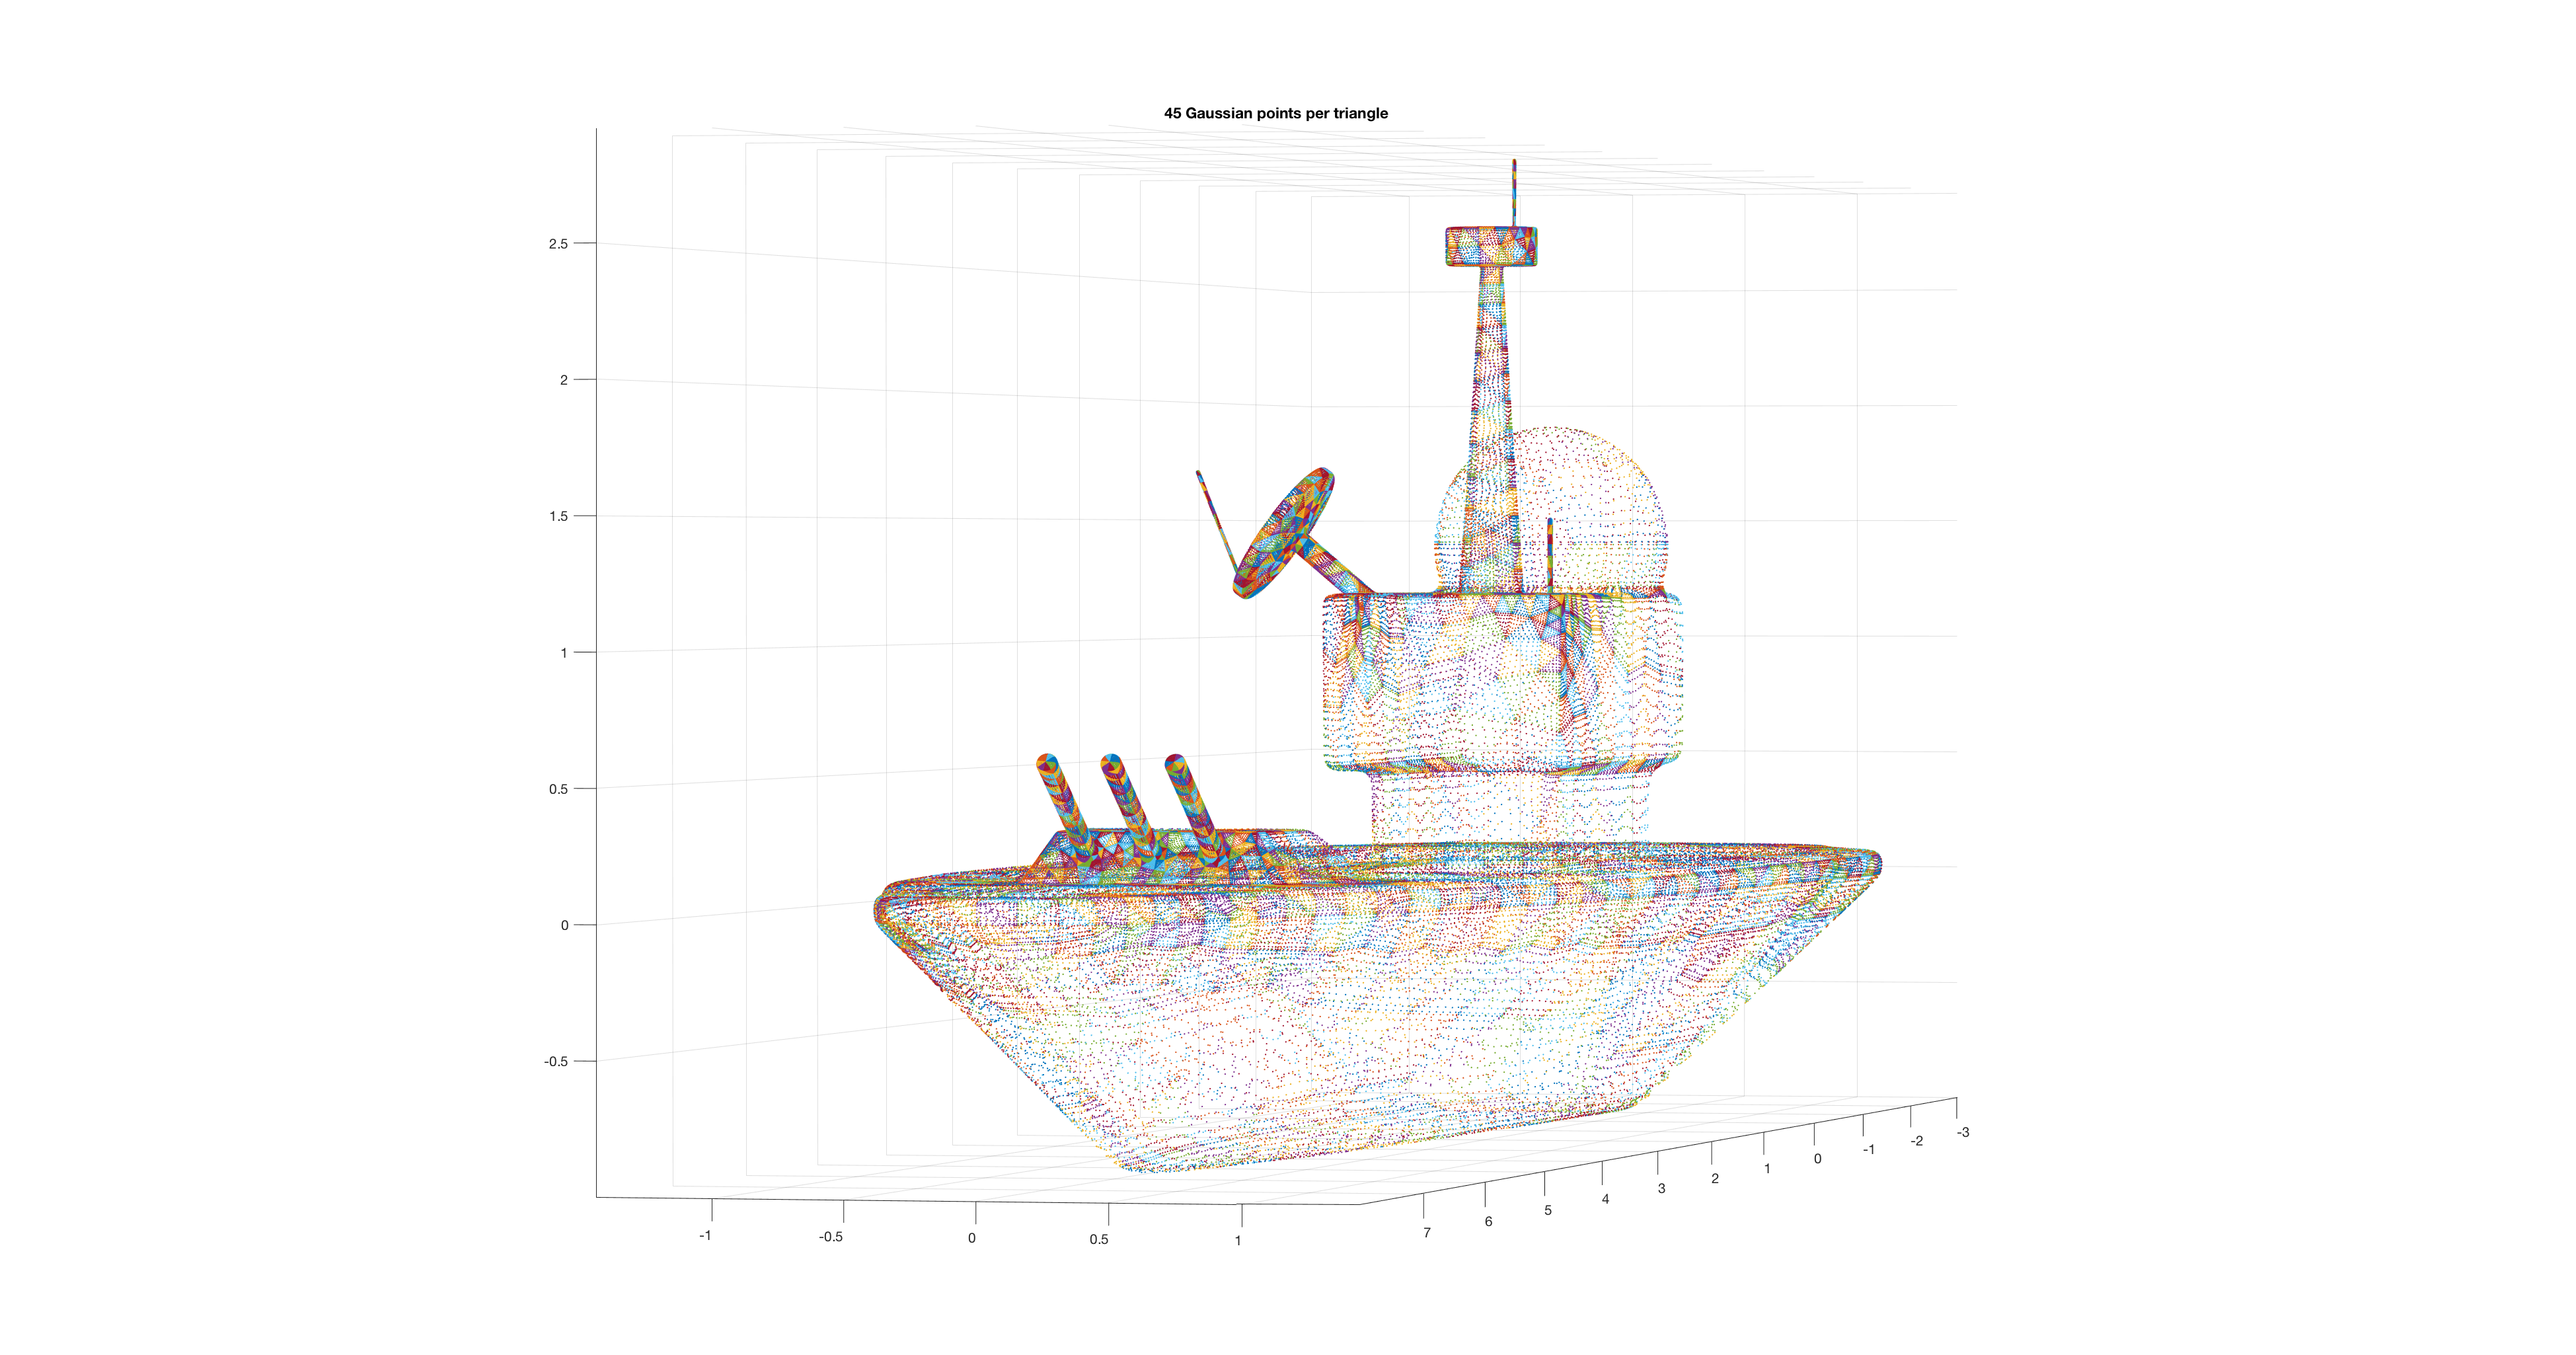
\includegraphics[width=6in]{war_ship_3.pdf}
\end{center}
\caption{}
\label{war_ship_3}
\end{figure}


\begin{figure}[H]
\begin{center}
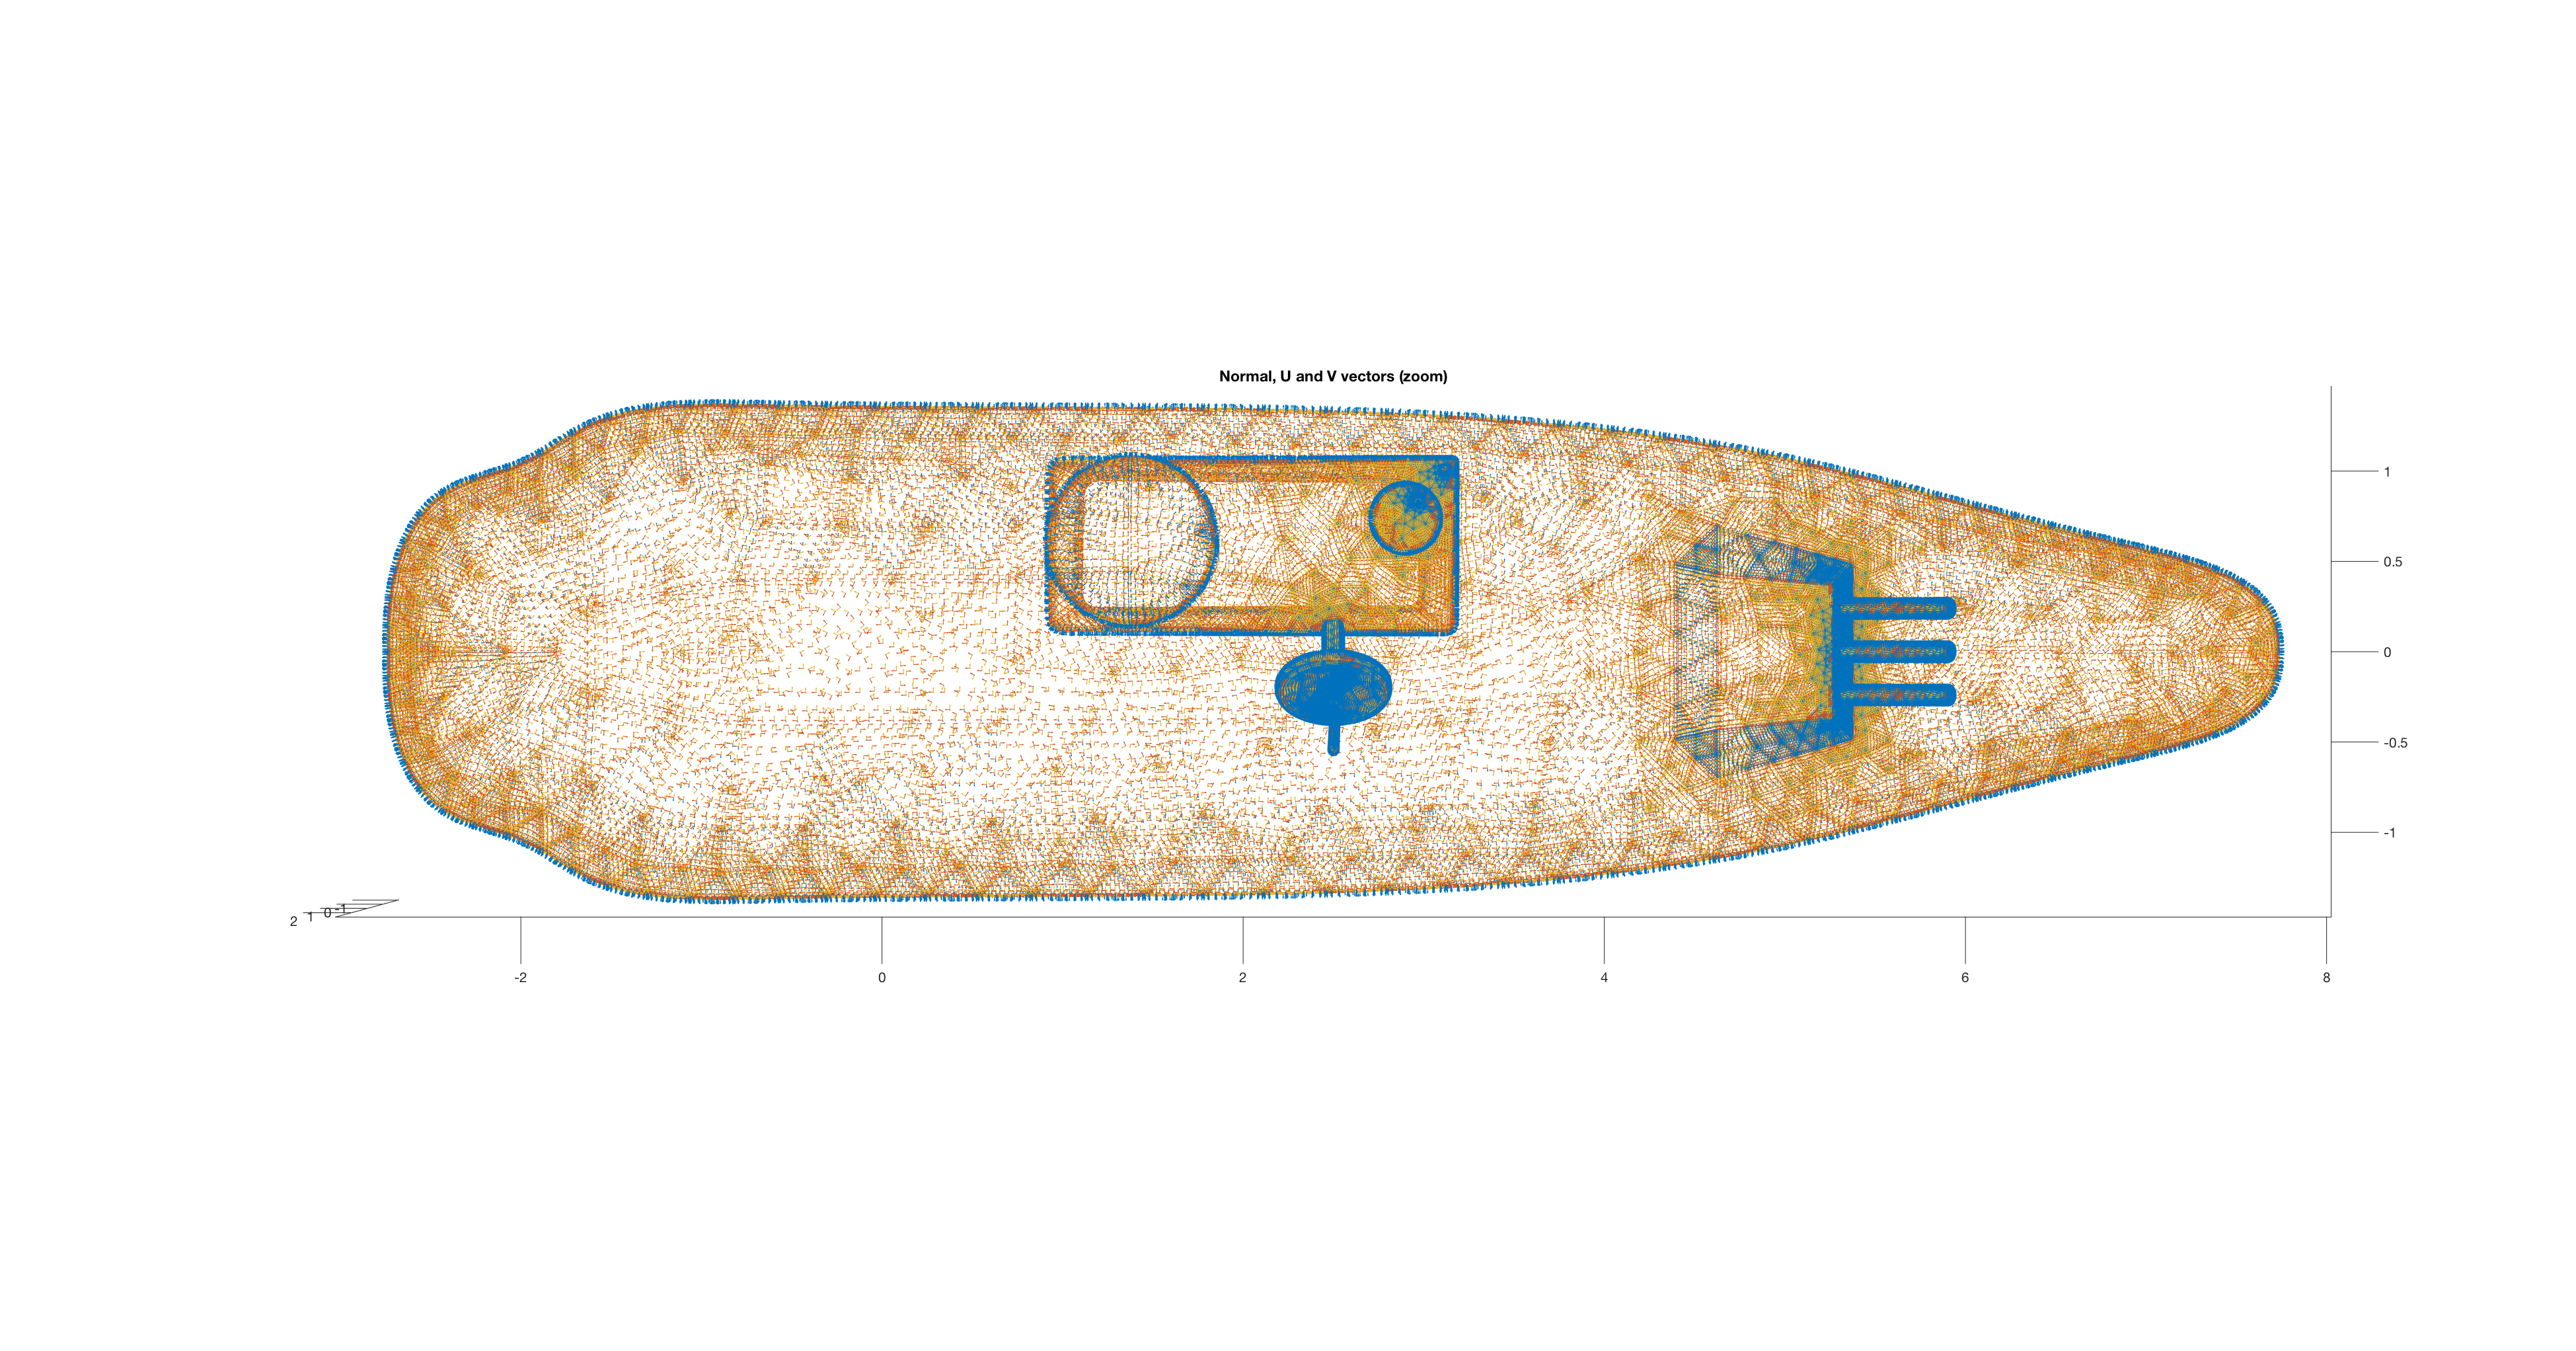
\includegraphics[width=6in]{war_ship_4.pdf}
\end{center}
\caption{}
\label{war_ship_4}
\end{figure}


\begin{figure}[H]
\begin{center}
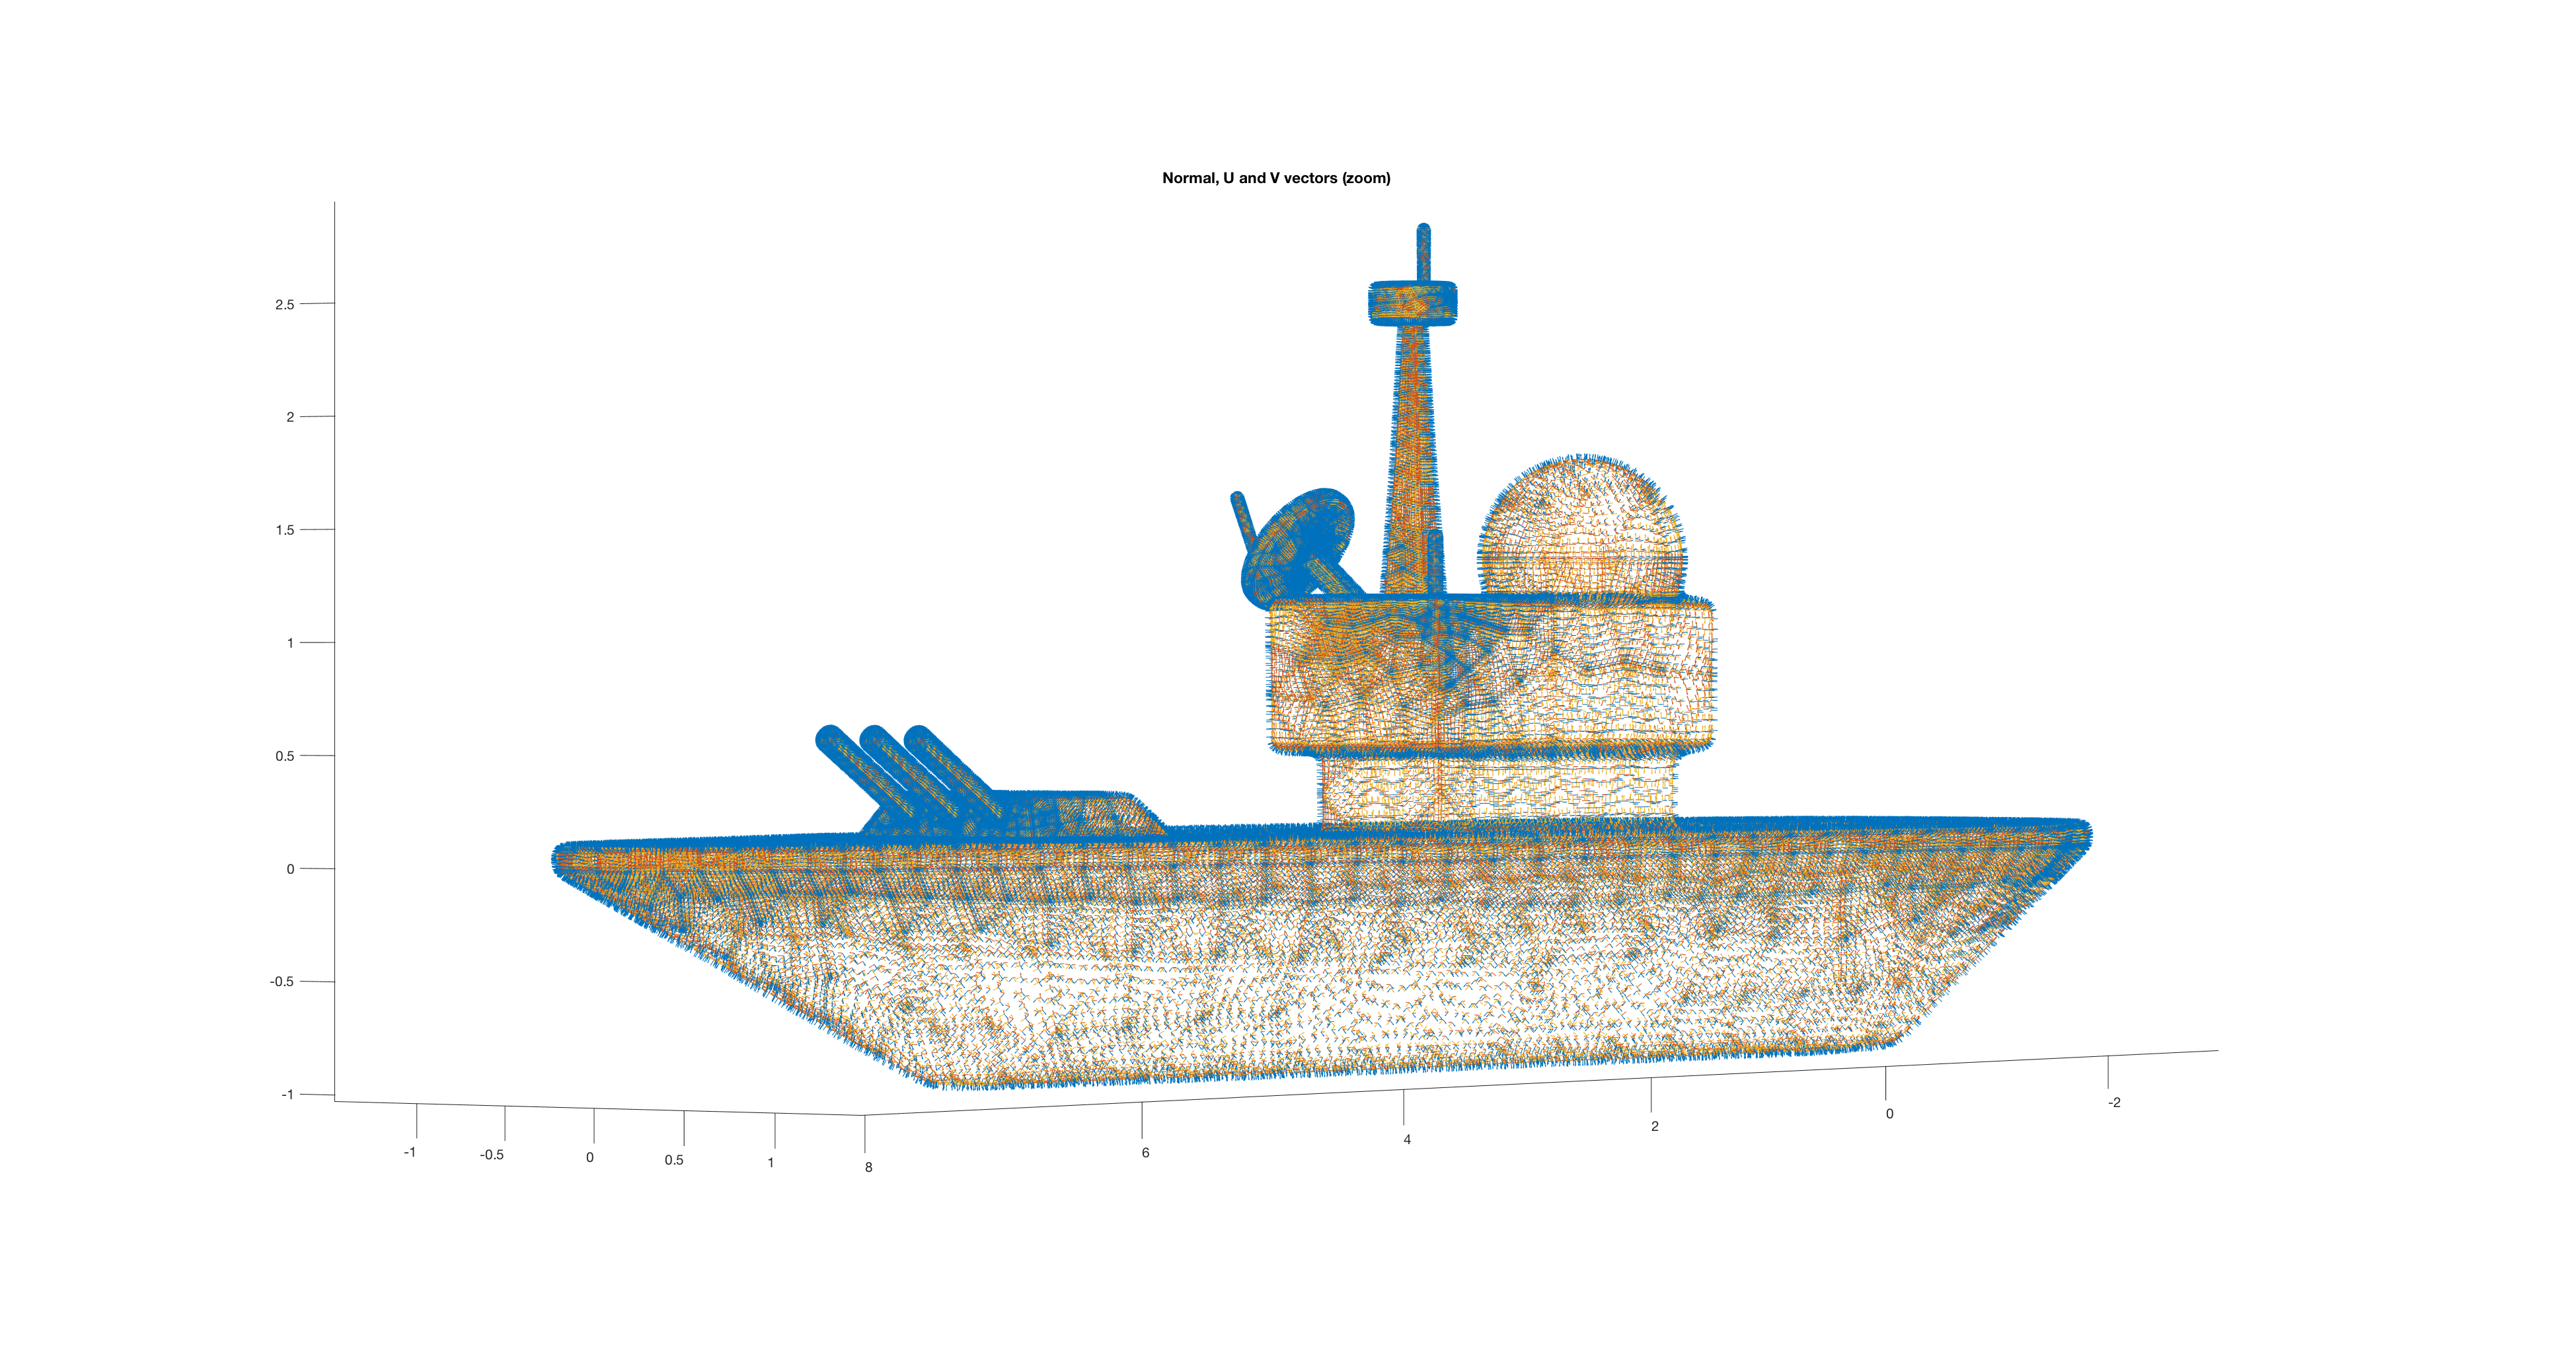
\includegraphics[width=6in]{war_ship_5.pdf}
\end{center}
\caption{}
\label{war_ship_5}
\end{figure}





  
\end{document}  